% Options for packages loaded elsewhere
\PassOptionsToPackage{unicode}{hyperref}
\PassOptionsToPackage{hyphens}{url}
%
\documentclass[
]{book}
\usepackage{amsmath,amssymb}
\usepackage{lmodern}
\usepackage{iftex}
\ifPDFTeX
  \usepackage[T1]{fontenc}
  \usepackage[utf8]{inputenc}
  \usepackage{textcomp} % provide euro and other symbols
\else % if luatex or xetex
  \usepackage{unicode-math}
  \defaultfontfeatures{Scale=MatchLowercase}
  \defaultfontfeatures[\rmfamily]{Ligatures=TeX,Scale=1}
\fi
% Use upquote if available, for straight quotes in verbatim environments
\IfFileExists{upquote.sty}{\usepackage{upquote}}{}
\IfFileExists{microtype.sty}{% use microtype if available
  \usepackage[]{microtype}
  \UseMicrotypeSet[protrusion]{basicmath} % disable protrusion for tt fonts
}{}
\makeatletter
\@ifundefined{KOMAClassName}{% if non-KOMA class
  \IfFileExists{parskip.sty}{%
    \usepackage{parskip}
  }{% else
    \setlength{\parindent}{0pt}
    \setlength{\parskip}{6pt plus 2pt minus 1pt}}
}{% if KOMA class
  \KOMAoptions{parskip=half}}
\makeatother
\usepackage{xcolor}
\usepackage{color}
\usepackage{fancyvrb}
\newcommand{\VerbBar}{|}
\newcommand{\VERB}{\Verb[commandchars=\\\{\}]}
\DefineVerbatimEnvironment{Highlighting}{Verbatim}{commandchars=\\\{\}}
% Add ',fontsize=\small' for more characters per line
\usepackage{framed}
\definecolor{shadecolor}{RGB}{248,248,248}
\newenvironment{Shaded}{\begin{snugshade}}{\end{snugshade}}
\newcommand{\AlertTok}[1]{\textcolor[rgb]{0.94,0.16,0.16}{#1}}
\newcommand{\AnnotationTok}[1]{\textcolor[rgb]{0.56,0.35,0.01}{\textbf{\textit{#1}}}}
\newcommand{\AttributeTok}[1]{\textcolor[rgb]{0.77,0.63,0.00}{#1}}
\newcommand{\BaseNTok}[1]{\textcolor[rgb]{0.00,0.00,0.81}{#1}}
\newcommand{\BuiltInTok}[1]{#1}
\newcommand{\CharTok}[1]{\textcolor[rgb]{0.31,0.60,0.02}{#1}}
\newcommand{\CommentTok}[1]{\textcolor[rgb]{0.56,0.35,0.01}{\textit{#1}}}
\newcommand{\CommentVarTok}[1]{\textcolor[rgb]{0.56,0.35,0.01}{\textbf{\textit{#1}}}}
\newcommand{\ConstantTok}[1]{\textcolor[rgb]{0.00,0.00,0.00}{#1}}
\newcommand{\ControlFlowTok}[1]{\textcolor[rgb]{0.13,0.29,0.53}{\textbf{#1}}}
\newcommand{\DataTypeTok}[1]{\textcolor[rgb]{0.13,0.29,0.53}{#1}}
\newcommand{\DecValTok}[1]{\textcolor[rgb]{0.00,0.00,0.81}{#1}}
\newcommand{\DocumentationTok}[1]{\textcolor[rgb]{0.56,0.35,0.01}{\textbf{\textit{#1}}}}
\newcommand{\ErrorTok}[1]{\textcolor[rgb]{0.64,0.00,0.00}{\textbf{#1}}}
\newcommand{\ExtensionTok}[1]{#1}
\newcommand{\FloatTok}[1]{\textcolor[rgb]{0.00,0.00,0.81}{#1}}
\newcommand{\FunctionTok}[1]{\textcolor[rgb]{0.00,0.00,0.00}{#1}}
\newcommand{\ImportTok}[1]{#1}
\newcommand{\InformationTok}[1]{\textcolor[rgb]{0.56,0.35,0.01}{\textbf{\textit{#1}}}}
\newcommand{\KeywordTok}[1]{\textcolor[rgb]{0.13,0.29,0.53}{\textbf{#1}}}
\newcommand{\NormalTok}[1]{#1}
\newcommand{\OperatorTok}[1]{\textcolor[rgb]{0.81,0.36,0.00}{\textbf{#1}}}
\newcommand{\OtherTok}[1]{\textcolor[rgb]{0.56,0.35,0.01}{#1}}
\newcommand{\PreprocessorTok}[1]{\textcolor[rgb]{0.56,0.35,0.01}{\textit{#1}}}
\newcommand{\RegionMarkerTok}[1]{#1}
\newcommand{\SpecialCharTok}[1]{\textcolor[rgb]{0.00,0.00,0.00}{#1}}
\newcommand{\SpecialStringTok}[1]{\textcolor[rgb]{0.31,0.60,0.02}{#1}}
\newcommand{\StringTok}[1]{\textcolor[rgb]{0.31,0.60,0.02}{#1}}
\newcommand{\VariableTok}[1]{\textcolor[rgb]{0.00,0.00,0.00}{#1}}
\newcommand{\VerbatimStringTok}[1]{\textcolor[rgb]{0.31,0.60,0.02}{#1}}
\newcommand{\WarningTok}[1]{\textcolor[rgb]{0.56,0.35,0.01}{\textbf{\textit{#1}}}}
\usepackage{longtable,booktabs,array}
\usepackage{calc} % for calculating minipage widths
% Correct order of tables after \paragraph or \subparagraph
\usepackage{etoolbox}
\makeatletter
\patchcmd\longtable{\par}{\if@noskipsec\mbox{}\fi\par}{}{}
\makeatother
% Allow footnotes in longtable head/foot
\IfFileExists{footnotehyper.sty}{\usepackage{footnotehyper}}{\usepackage{footnote}}
\makesavenoteenv{longtable}
\usepackage{graphicx}
\makeatletter
\def\maxwidth{\ifdim\Gin@nat@width>\linewidth\linewidth\else\Gin@nat@width\fi}
\def\maxheight{\ifdim\Gin@nat@height>\textheight\textheight\else\Gin@nat@height\fi}
\makeatother
% Scale images if necessary, so that they will not overflow the page
% margins by default, and it is still possible to overwrite the defaults
% using explicit options in \includegraphics[width, height, ...]{}
\setkeys{Gin}{width=\maxwidth,height=\maxheight,keepaspectratio}
% Set default figure placement to htbp
\makeatletter
\def\fps@figure{htbp}
\makeatother
\setlength{\emergencystretch}{3em} % prevent overfull lines
\providecommand{\tightlist}{%
  \setlength{\itemsep}{0pt}\setlength{\parskip}{0pt}}
\setcounter{secnumdepth}{5}
\usepackage{booktabs}
\usepackage{fontspec}
\usepackage{multirow}
\usepackage{multicol}
\usepackage{colortbl}
\usepackage{hhline}
\usepackage{longtable}
\usepackage{array}
\usepackage{hyperref}
\ifLuaTeX
  \usepackage{selnolig}  % disable illegal ligatures
\fi
\usepackage[]{natbib}
\bibliographystyle{apalike}
\IfFileExists{bookmark.sty}{\usepackage{bookmark}}{\usepackage{hyperref}}
\IfFileExists{xurl.sty}{\usepackage{xurl}}{} % add URL line breaks if available
\urlstyle{same} % disable monospaced font for URLs
\hypersetup{
  pdftitle={Einführung in R},
  pdfauthor={Stephan Goerigk},
  hidelinks,
  pdfcreator={LaTeX via pandoc}}

\title{Einführung in R}
\author{Stephan Goerigk}
\date{2023-05-18}

\begin{document}
\maketitle

{
\setcounter{tocdepth}{1}
\tableofcontents
}
\hypertarget{uxfcber-dieses-skript}{%
\chapter*{Über dieses Skript}\label{uxfcber-dieses-skript}}
\addcontentsline{toc}{chapter}{Über dieses Skript}

Liebe Studierende,

dieses Skript soll Sie in die grundlegenden Analysewerkzeuge in R einführen, von der grundlegenden Kodierung und Analyse bis hin zur Datenverarbeitung, dem Plotten und der statistischen Inferenz.

Wenn R Ihre erste Programmiersprache ist, ist das völlig in Ordnung. Wir gehen alles Schritt für Schritt gemeinsam durch. Die Techniken in diesem Skript sind zwar auf die meisten Datenanalyseprobleme anwendbar, da wir jedoch aus der Psychologie kommen, werde ich den Kurs auf die Lösung von Analyseproblemen ausrichten, die in der psychologischen Forschung häufig auftreten.

Ich wünsche Ihnen Viel Erfolg und Spaß!

\hypertarget{warum-ist-r-empfehlenswert}{%
\chapter{Warum ist R empfehlenswert?}\label{warum-ist-r-empfehlenswert}}

\hypertarget{open-source}{%
\section{Open Source}\label{open-source}}

Im Gegensatz zu SPSS, Matlab, Excel und JMP ist R kostenlos und verfügt über eine große Unterstützergemeinschaft. Das bedeutet, dass eine große Gemeinschaft von R-Programmierer:innen ständig neue R-Funktionen und -Pakete entwickelt und verbreitet. Wenn Sie jemals eine Frage dazu haben, wie man etwas in R implementiert, wird eine schnelle Suche im Internet Sie praktisch jedes Mal zur Antwort führen.

\hypertarget{vielseitigkeit}{%
\section{Vielseitigkeit}\label{vielseitigkeit}}

R ist sehr vielseitig. Sie können R für alles verwenden, von der Berechnung einfacher zusammenfassender Statistiken über die Durchführung komplexer Simulationen bis hin zur Erstellung von Diagrammen. Wenn Sie sich eine statistische Aufgabe vorstellen können, können Sie sie mit ziemlicher Sicherheit in R implementieren.

\hypertarget{rmarkdown}{%
\section{RMarkdown}\label{rmarkdown}}

Mit RStudio, einem Programm, das Sie beim Schreiben von R-Code unterstützt, können Sie mittels RMarkdown einfach und nahtlos R-Code, Analysen, Diagramme und geschriebenen Text zu eleganten Dokumenten an einem Ort kombinieren. Tatsächlich wurde dieses gesamte Skript (Text, Formatierung, Diagramme, Code\ldots) in RStudio mit R Markdown geschrieben. Mit RStudio müssen Sie sich nicht mehr mit zwei oder drei Programmen herumschlagen, z. B. Excel, Word und SPSS, wo Sie die Hälfte Ihrer Zeit mit dem Kopieren, Einfügen und Formatieren von Daten, Bildern und Tests verbringen, sondern können alles an einem Ort erledigen, so dass nichts mehr falsch gelesen, getippt oder vergessen wird.

\hypertarget{transparenz}{%
\section{Transparenz}\label{transparenz}}

In R durchgeführte Analysen sind transparent, leicht weiterzugeben und reproduzierbar. Wenn Sie einen SPSS-Benutzer fragen, wie er eine bestimmte Analyse durchgeführt hat, wird er sich ggf. nicht daran erinnern, was er vor Monaten oder Jahren tatsächlich getan hat. Wenn Sie eine R-Anwender:in (der/die gute Programmiertechniken verwendet) fragen, wie er/sie eine Analyse durchgeführt hat, sollte er/sie Ihnen immer den genauen Code zeigen können, den er/sie verwendet hat. Das bedeutet natürlich nicht, dass er/sie die richtige Analyse verwendet oder sie korrekt interpretiert hat, aber mit dem gesamten Originalcode sollten etwaige Probleme völlig transparent sein! Dies ist eine Grundvoraussetzung für offene, replizierbare Forschung.

\hypertarget{r-materialien}{%
\chapter{R Materialien}\label{r-materialien}}

\hypertarget{cheat-sheets}{%
\section{Cheat Sheets}\label{cheat-sheets}}

In diesem Skript werden Sie viele neue Funktionen kennenlernen. Wäre es nicht schön, wenn jemand ein Wörterbuch mit vielen gängigen R-Funktionen erstellen würde? Im Folgenden finden Sie eine Tabelle mit einigen der Funktionen, die ich empfehle. Ich empfehle Ihnen dringend, diese auszudrucken und die Funktionen zu markieren, wenn Sie sie lernen!

\href{https://cran.r-project.org/doc/contrib/Short-refcard.pdf}{Link zum Base R Cheat Sheet}

\href{https://www.rstudio.com/resources/cheatsheets/}{Link zu den R Studio Cheat Sheets}

Insbesondere die Cheat Sheets zu ggplot2 und dplyr sind zu empfehlen (RStudio Cheat Sheets S.2).

\hypertarget{hilfe-und-inspiration-online}{%
\section{Hilfe und Inspiration online}\label{hilfe-und-inspiration-online}}

Eine Internetsuche nach einem spezifischen R Problem bringt Sie (fast) immer an Ihr Ziel. Häufig findet man gute Antworten in den github Hilfsmatierialien einzelner Pakete, auf den Community Seiten von R Studio und in den Foren von stackoverflow.

\hypertarget{andere-buxfccher}{%
\section{Andere Bücher}\label{andere-buxfccher}}

Die Inhalte dieser Bücher sind nicht prüfunsrelevant.

Es gibt viele, viele gute Bücher über R. Hier sind zwei, die ich empfehlen kann (von denen eines sogar umsonst ist):

\href{https://www.amazon.com/Discovering-Statistics-Using-Andy-Field/dp/1446200469/ref=sr_1_2?ie=UTF8\&qid=1487759316\&sr=8-2\&keywords=statistics+with+r}{Discovering Statistics with R von Field, Miles and Field}

\href{http://r4ds.had.co.nz}{R for Data Science von Garrett Grolemund and Hadley Wickham}

\hypertarget{installation}{%
\chapter{Installation}\label{installation}}

Um R benutzen zu können, müssen wir zwei Softwarepakete herunterladen:

\begin{itemize}
\tightlist
\item
  \textbf{R}
\item
  \textbf{RStudio}
\end{itemize}

R ist die Programmiersprache, mit der wir arbeiten. R-Studio ist eine Benutzeroberfläche, die uns das Programmieren mit R ungemein erleichtert.

\hypertarget{installation-von-r}{%
\section{Installation von R}\label{installation-von-r}}

Um R zu installieren, klicken Sie auf den Ihrem Betriebssystem entsprechenden Link und befolgen Sie die Anleitungen.

\begin{longtable}[]{@{}
  >{\raggedright\arraybackslash}p{(\columnwidth - 2\tabcolsep) * \real{0.5833}}
  >{\raggedright\arraybackslash}p{(\columnwidth - 2\tabcolsep) * \real{0.4167}}@{}}
\toprule()
\begin{minipage}[b]{\linewidth}\raggedright
Operating System
\end{minipage} & \begin{minipage}[b]{\linewidth}\raggedright
Link
\end{minipage} \\
\midrule()
\endhead
Windows & \url{http://cran.r-project.org/bin/windows/base/} \\
Mac & \url{http://cran.r-project.org/bin/macosx/} \\
\bottomrule()
\end{longtable}

Nach dieser Installation haben Sie bereits die volle Funktionalität des Programms. Sie werden jedoch feststellen, dass beinahe alle R-Nutzer RStudio zum programmieren nutzen, da dieses eine leichter nutzbare Oberfläche hat.
Tatsächlich müssen Sie nach der Installation von RStudio das R Basisprogramm nie wieder öffnen.

\hypertarget{installation-von-rstudio}{%
\section{Installation von RStudio}\label{installation-von-rstudio}}

Bitte installieren Sie dann RStudio - das Programm, über welches wir auf R zugreifen und mit dem wir unsere Skripte schreiben.

Um RStudio zu installieren, klicken Sie auf diesen Link und befolgen Sie die Anleitungen: \url{http://www.rstudio.com/products/rstudio/download/}

\hypertarget{programmaufbau}{%
\chapter{Programmaufbau}\label{programmaufbau}}

\hypertarget{die-vier-rstudio-fenster}{%
\section{Die vier RStudio Fenster}\label{die-vier-rstudio-fenster}}

Wenn Sie RStudio öffnen, sehen Sie vier Fenster, wie in der folgenden Abbildung dargestellt:

\begin{figure}
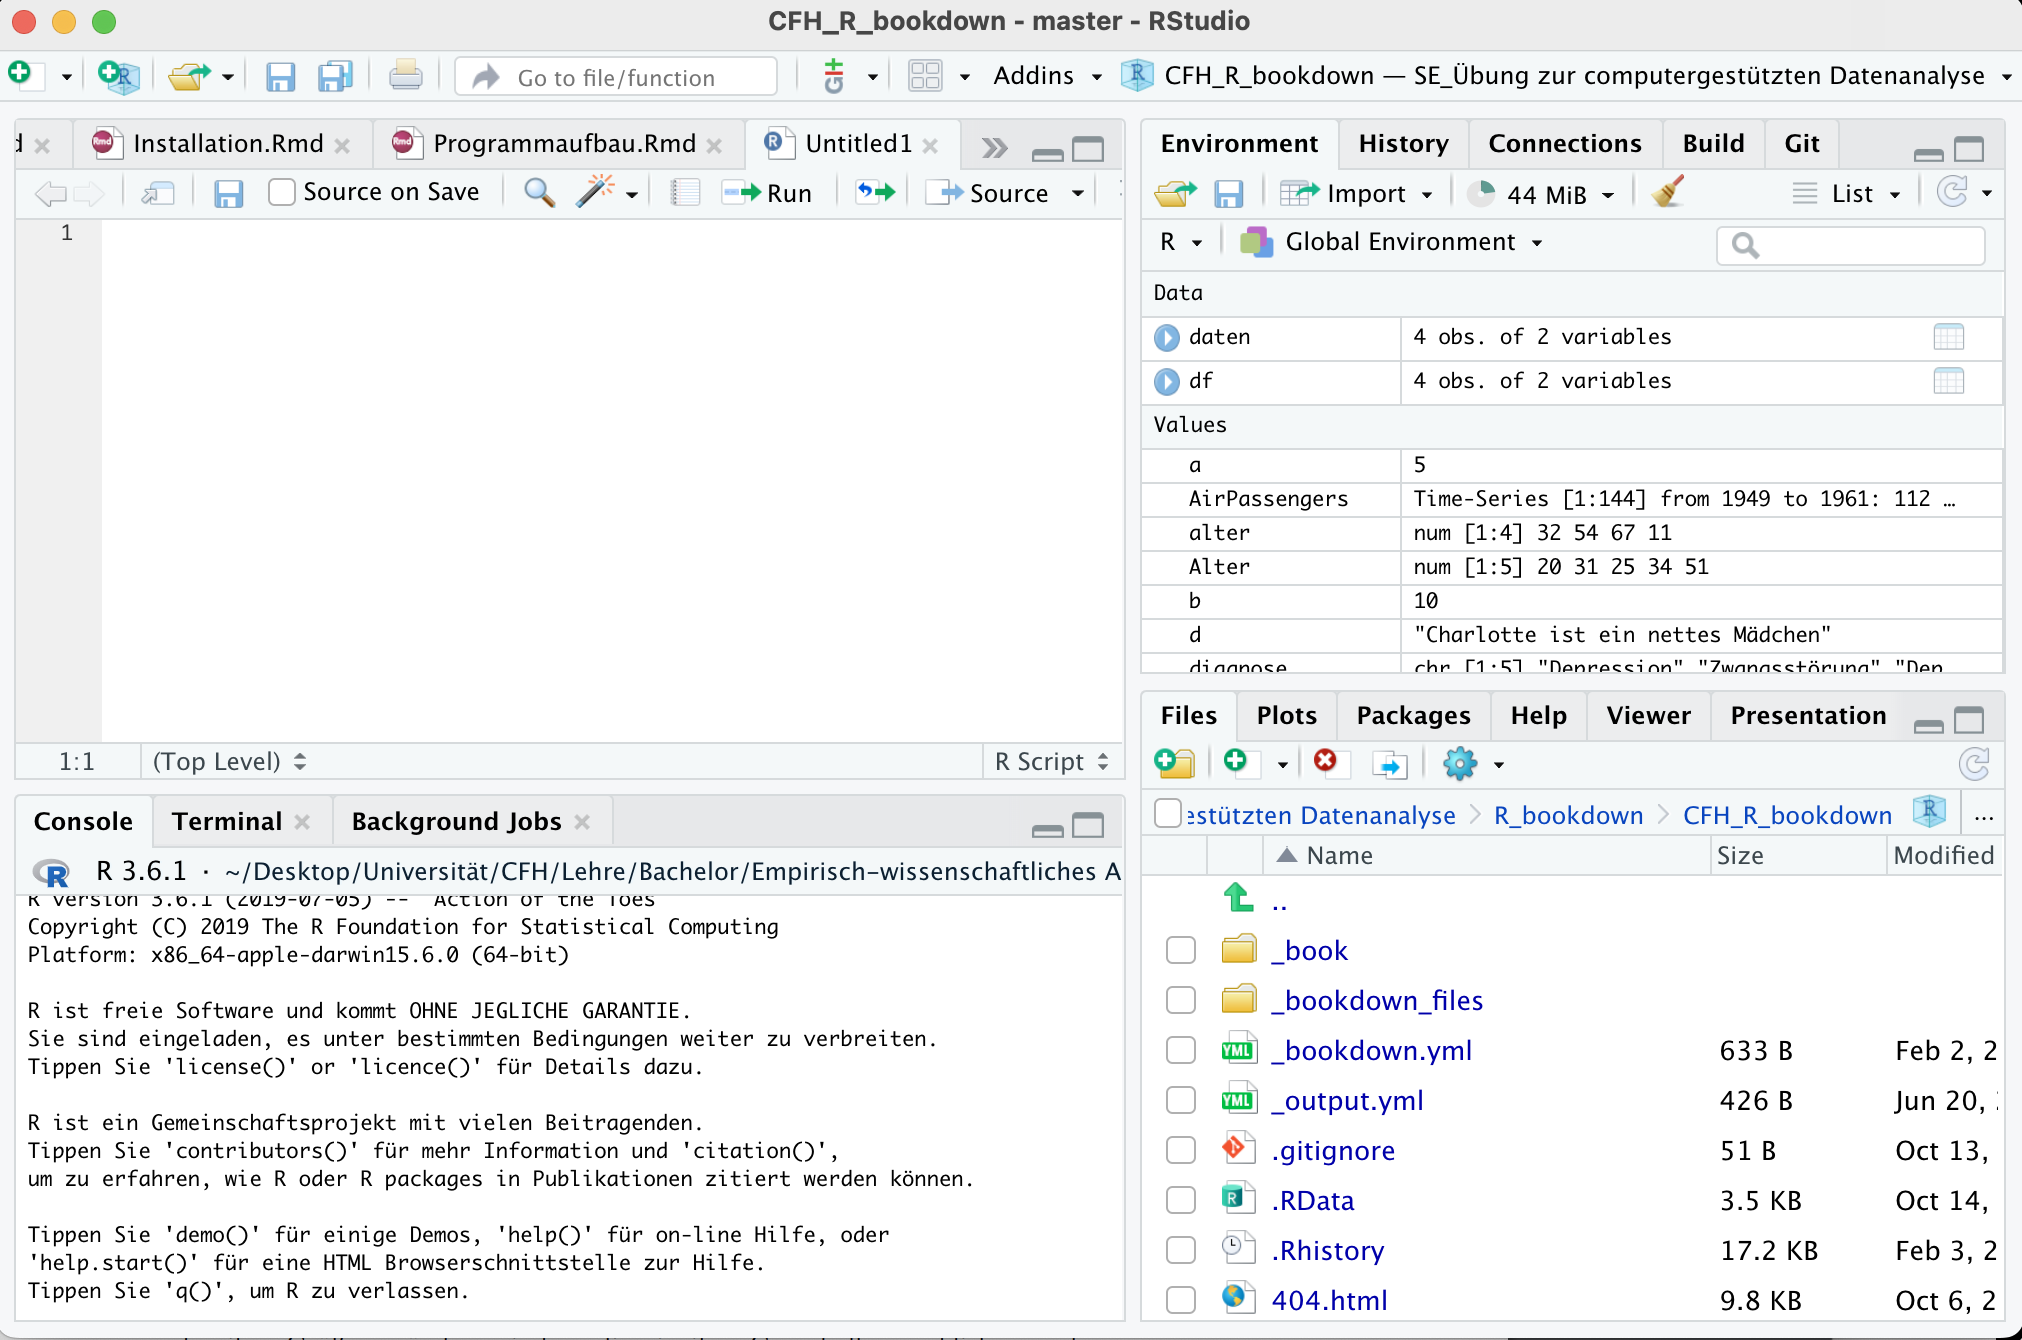
\includegraphics[width=28.08in]{images/windows} \caption{Die vier RStudio Fenster}\label{fig:unnamed-chunk-1}
\end{figure}

Wenn Sie mögen, können Sie die Reihenfolge der Fenster in den RStudio Einstellungen verändern.
Sie können die Fenster auch verstecken (Minimieren/Maximieren Symbol an der oberen rechten Ecke jedes Fensters) oder ihre Größe verändern, indem die sie ihre Grenzbalken anklicken und verschieben.

Lassen Sie uns jetzt schauen, was genau die Funktion jedes der Fenster ist:

\hypertarget{source---ihr-schreibblock-fuxfcr-code}{%
\subsection{Source - Ihr Schreibblock für Code}\label{source---ihr-schreibblock-fuxfcr-code}}

Im Source Fenster erstellen und bearbeiten Sie ``R-Skripte'' - Ihre Codesammlungen. Keine Sorge, R-Skripte sind nur Textdateien mit der Erweiterung ``.R''.
Wenn Sie RStudio öffnen, wird automatisch ein neues unbenanntes Skript gestartet.
Bevor Sie mit der Eingabe eines unbenannten R-Skripts beginnen, sollten Sie die Datei immer unter einem neuen Dateinamen speichern (z.B. ``Mein\_RScript.R'').
Wenn Ihr Computer während der Arbeit abstürzt, steht Ihr Code in R zur Verfügung, wenn Sie RStudio erneut öffnen.

\begin{figure}
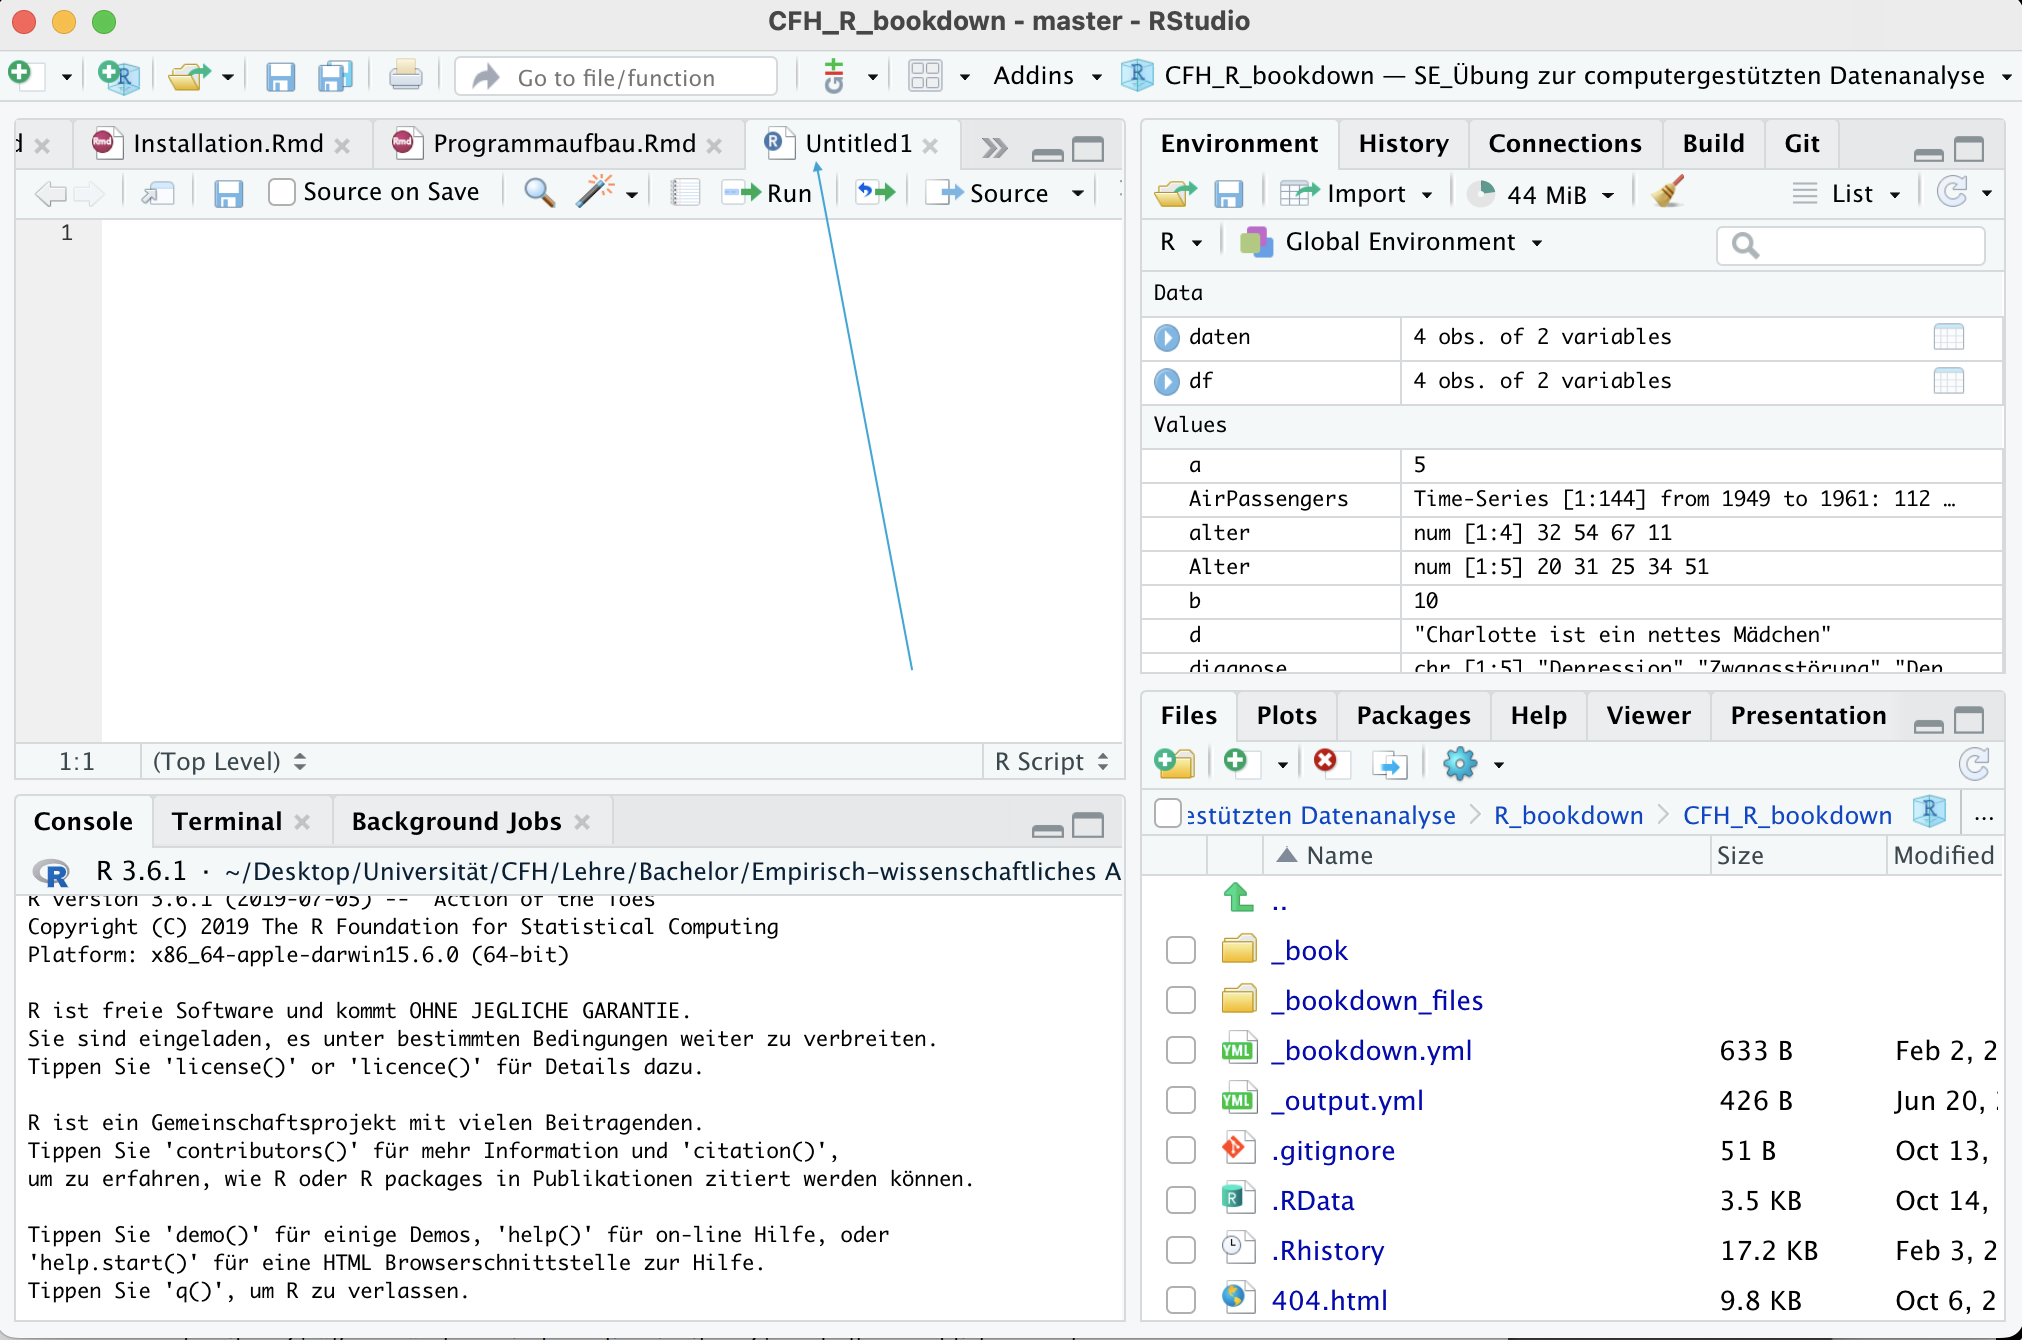
\includegraphics[width=28.08in]{images/windows_source} \caption{Die vier RStudio Fenster}\label{fig:unnamed-chunk-2}
\end{figure}

Sie werden feststellen, dass R beim Schreiben des Skripts den Code während der Eingabe nicht tatsächlich ausführt. Damit R Ihren Code tatsächlich ausführt, müssen Sie den Code zunächst an die Konsole ``senden'' (wir werden im nächsten Abschnitt darüber sprechen).

Es gibt viele Möglichkeiten, Ihren Code aus dem Skript an die Konsole zu senden. Die langsamste Methode ist das Kopieren und Einfügen. Schneller geht es, wenn Sie den Code, den Sie auswerten möchten, markieren und auf die Schaltfläche ``Run'' oben rechts in der Quelle klicken. Alternativ können Sie auch die Tastenkombination ``Command + Return'' auf dem Mac oder ``Control + Enter'' auf dem PC verwenden, um den gesamten markierten Code an die Konsole zu senden.

\hypertarget{konsole---das-herzstuxfcck-von-r}{%
\subsection{Konsole - Das Herzstück von R}\label{konsole---das-herzstuxfcck-von-r}}

Die Konsole ist das Herzstück von R. Hier führt R den Code aus. Am Anfang der Konsole sehen Sie das Zeichen ``\textgreater{}''. Dies ist eine Eingabeaufforderung (sog. ``Prompt''), die Ihnen mitteilt, dass R bereit für neuen Code ist. Sie können direkt nach dem Prompt \texttt{\textgreater{}} Code in die Konsole eingeben und erhalten sofort eine Antwort. Wenn Sie zum Beispiel 2+2 in die Konsole eingeben und die Eingabetaste drücken, werden Sie sehen, dass R sofort eine Ausgabe von 4 liefert.

\begin{Shaded}
\begin{Highlighting}[]
\DecValTok{2}\SpecialCharTok{+}\DecValTok{2}
\end{Highlighting}
\end{Shaded}

\begin{verbatim}
## [1] 4
\end{verbatim}

Versuchen Sie, 2+2 zu berechnen, indem Sie den Code direkt in die Konsole eingeben - und dann Enter drücken.
Sie sollten das Ergebnis \texttt{{[}1{]}\ 4} sehen. Machen Sie sich keine Gedanken über die \texttt{{[}1{]}}, dazu kommen wir später.

\begin{figure}
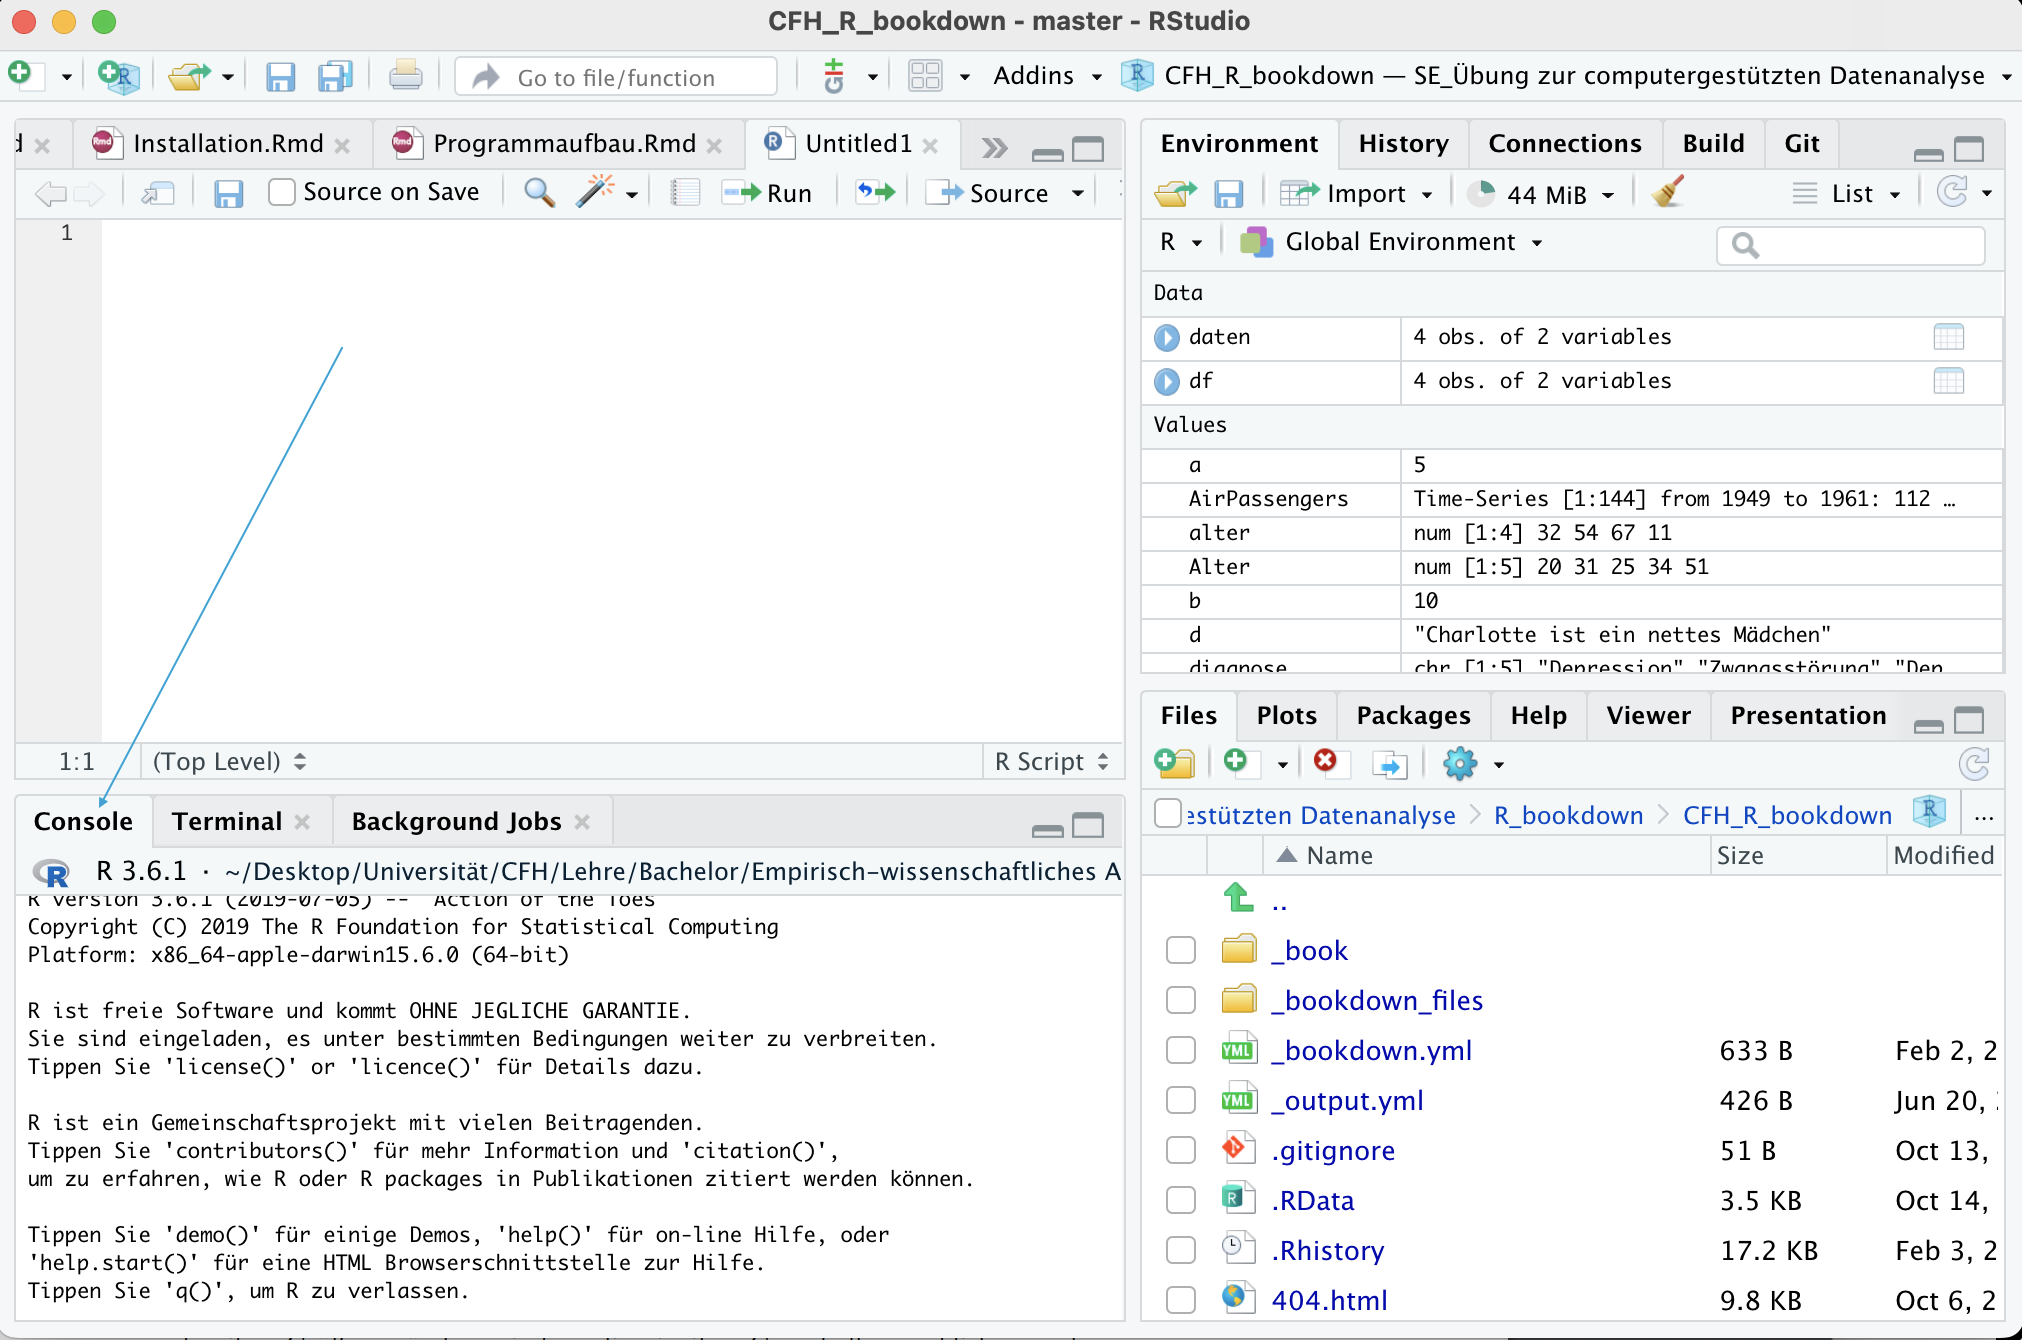
\includegraphics[width=28.08in]{images/windows_console} \caption{Die vier RStudio Fenster}\label{fig:unnamed-chunk-4}
\end{figure}

Geben Sie denselben Code in das Skript ein und senden Sie ihn an die Konsole, indem Sie den Code markieren und auf die Schaltfläche ``Run'' in der oberen rechten Ecke des Quelltextfensters klicken. Alternativ können Sie auch die Tastenkombination ``Command + Return'' auf dem Mac oder ``Control + Enter'' unter Windows verwenden.

\textbf{Tipp}: Wie Sie sehen, können Sie Code entweder über das Skript oder durch direkte Eingabe in die Konsole ausführen. In 99\% der Fälle sollten Sie jedoch das Skript und nicht die Konsole verwenden. Der Grund dafür ist ganz einfach: Wenn Sie den Code in die Konsole eingeben, wird er nicht gespeichert (obwohl Sie in Ihrem Befehlsverlauf nachsehen können). Und wenn Sie beim Eingeben von Code in die Konsole einen Fehler machen, müssen Sie alles noch einmal von vorne eingeben. Stattdessen ist es besser, den gesamten Code in das Skript zu schreiben. Wenn Sie bereit sind, einen Code auszuführen, können Sie ihn mit ``Run'' an die Konsole senden.

\hypertarget{environmenthistory---das-geduxe4chtnis-von-r}{%
\subsection{Environment/History - Das Gedächtnis von R}\label{environmenthistory---das-geduxe4chtnis-von-r}}

In dem Tab ``Environment'' dieses Bereichs werden die Namen aller Datenobjekte (wie Vektoren, Matrizen und Datenrahmen) angezeigt, die Sie in Ihrer aktuellen R-Session definiert haben. Sie können auch Informationen wie die Anzahl der Spalten und Zeilen in Datensätzen sehen. Der Tab enthält auch einige anklickbare Aktionen wie ``Datensatz importieren'', wodurch eine grafische Benutzeroberfläche (GUI) für wichtige Daten in R geöffnet wird.

\begin{figure}
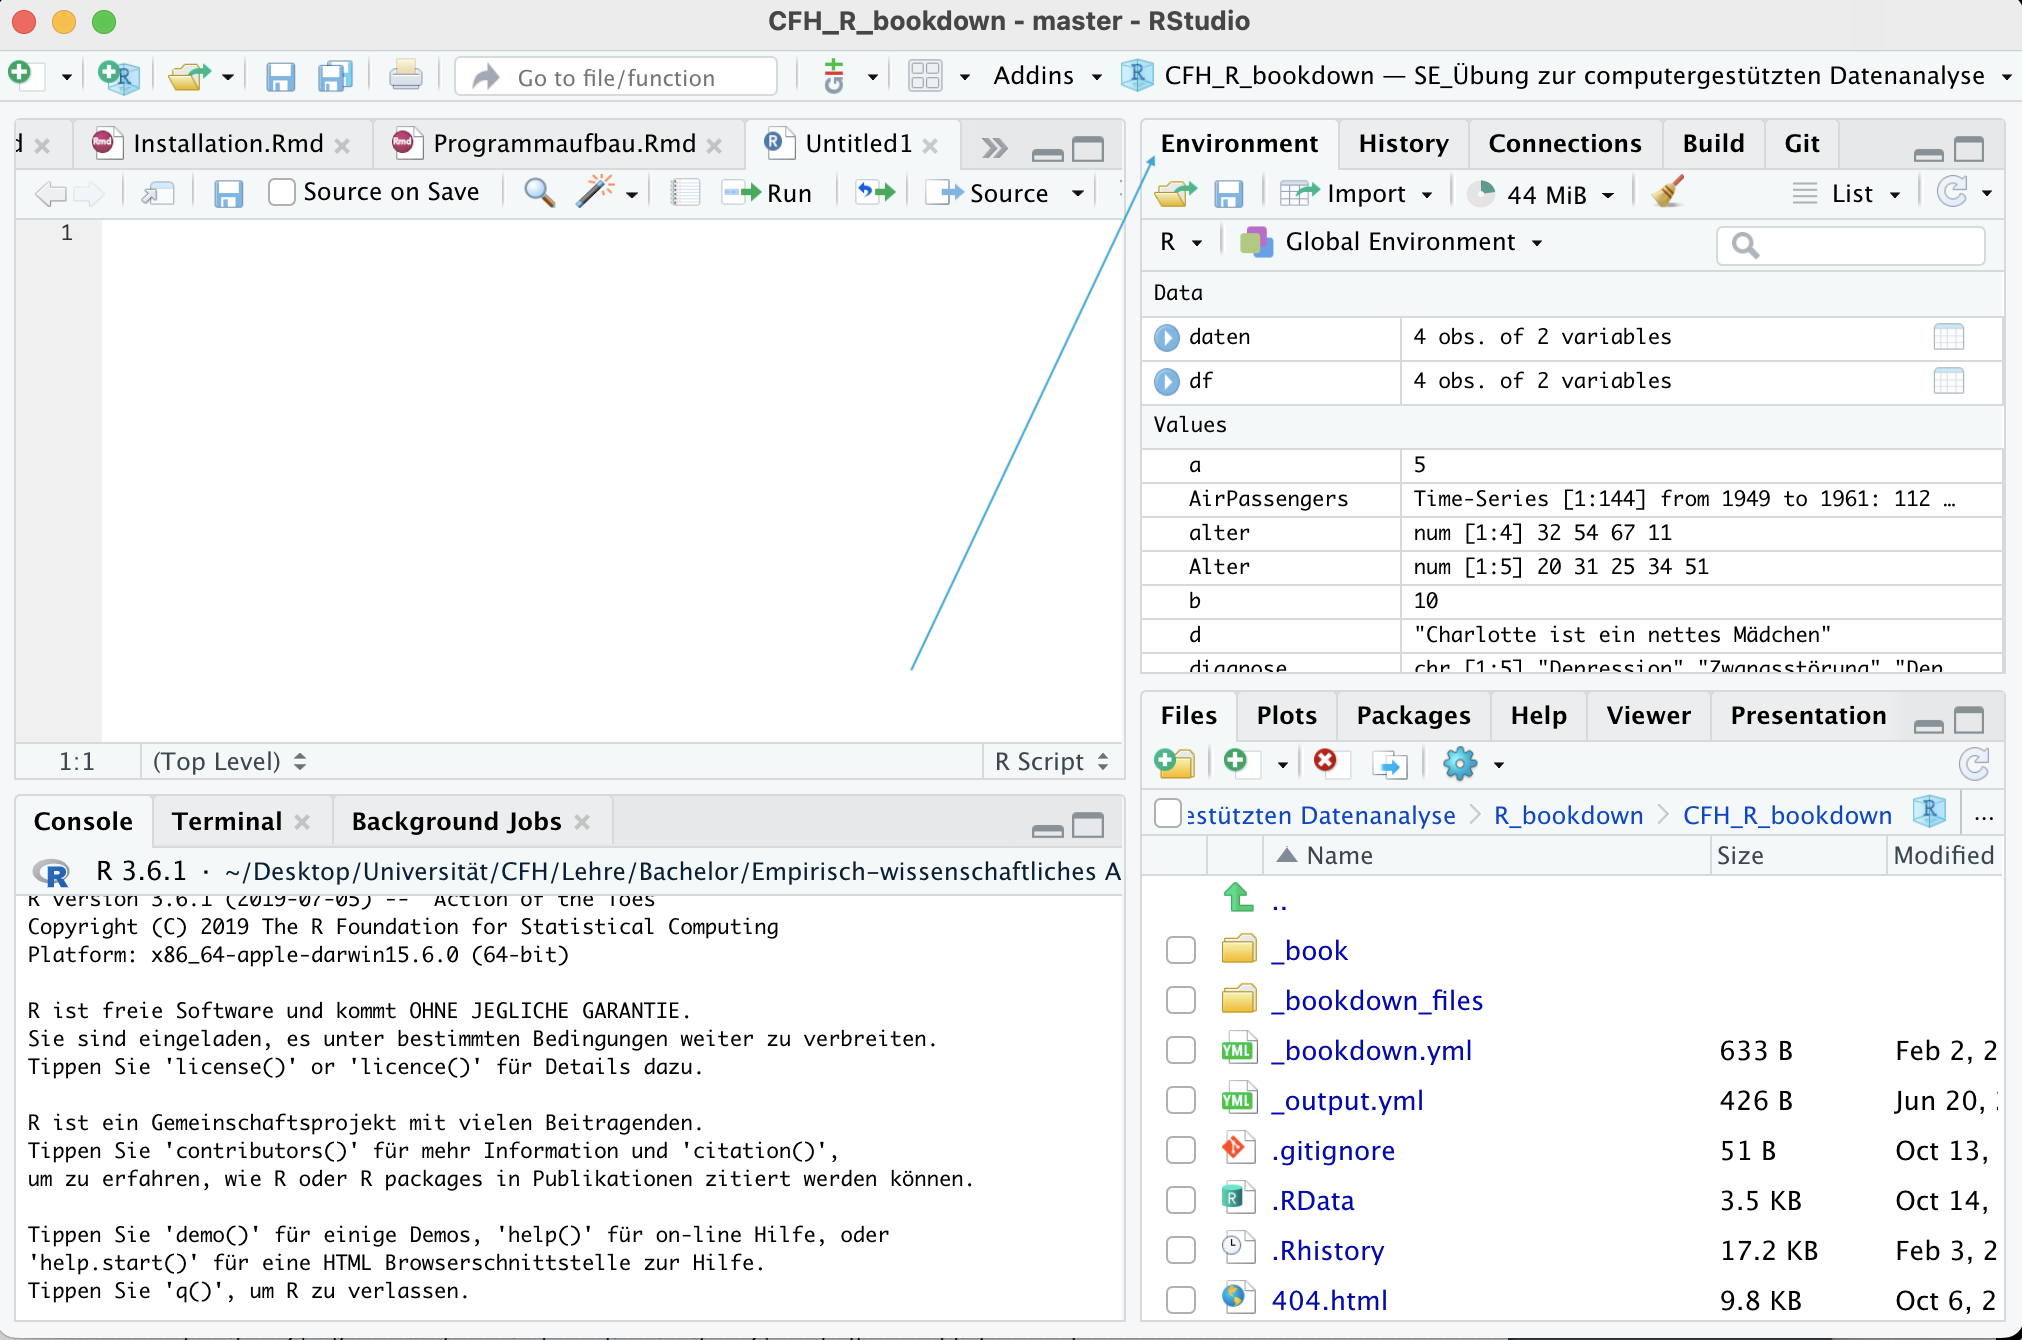
\includegraphics[width=28.08in]{images/windows_env} \caption{Die vier RStudio Fenster}\label{fig:unnamed-chunk-5}
\end{figure}

Der Tab ``History'' dieses Bereichs zeigt Ihnen einfach eine Sammlung aller Befehle an, die Sie zuvor in der Konsole ausgewertet haben. Wenn man mit Skripten arbeitet, schaut man sich diese allerdings relativ selten an.

Wenn Sie sich mit R besser auskennen, werden Sie das Fenster Environment/History vielleicht nützlich finden. Aber für den Moment können Sie es einfach ignorieren. Wenn Sie Ihren Bildschirm entrümpeln wollen, können Sie das Fenster auch einfach minimieren, indem Sie auf die Schaltfläche Minimieren oben rechts im Fenster klicken.

\hypertarget{filesplotspackageshelpviewer---interaktion-von-r-mit-dateien}{%
\subsection{Files/Plots/Packages/Help/Viewer - Interaktion von R mit Dateien}\label{filesplotspackageshelpviewer---interaktion-von-r-mit-dateien}}

Die Tabs Files/Plots/Packages/Help/Viewer zeigen Ihnen viele hilfreiche Informationen. Schauen wir uns die einzelnen Registerkarten im Detail an:

\begin{figure}
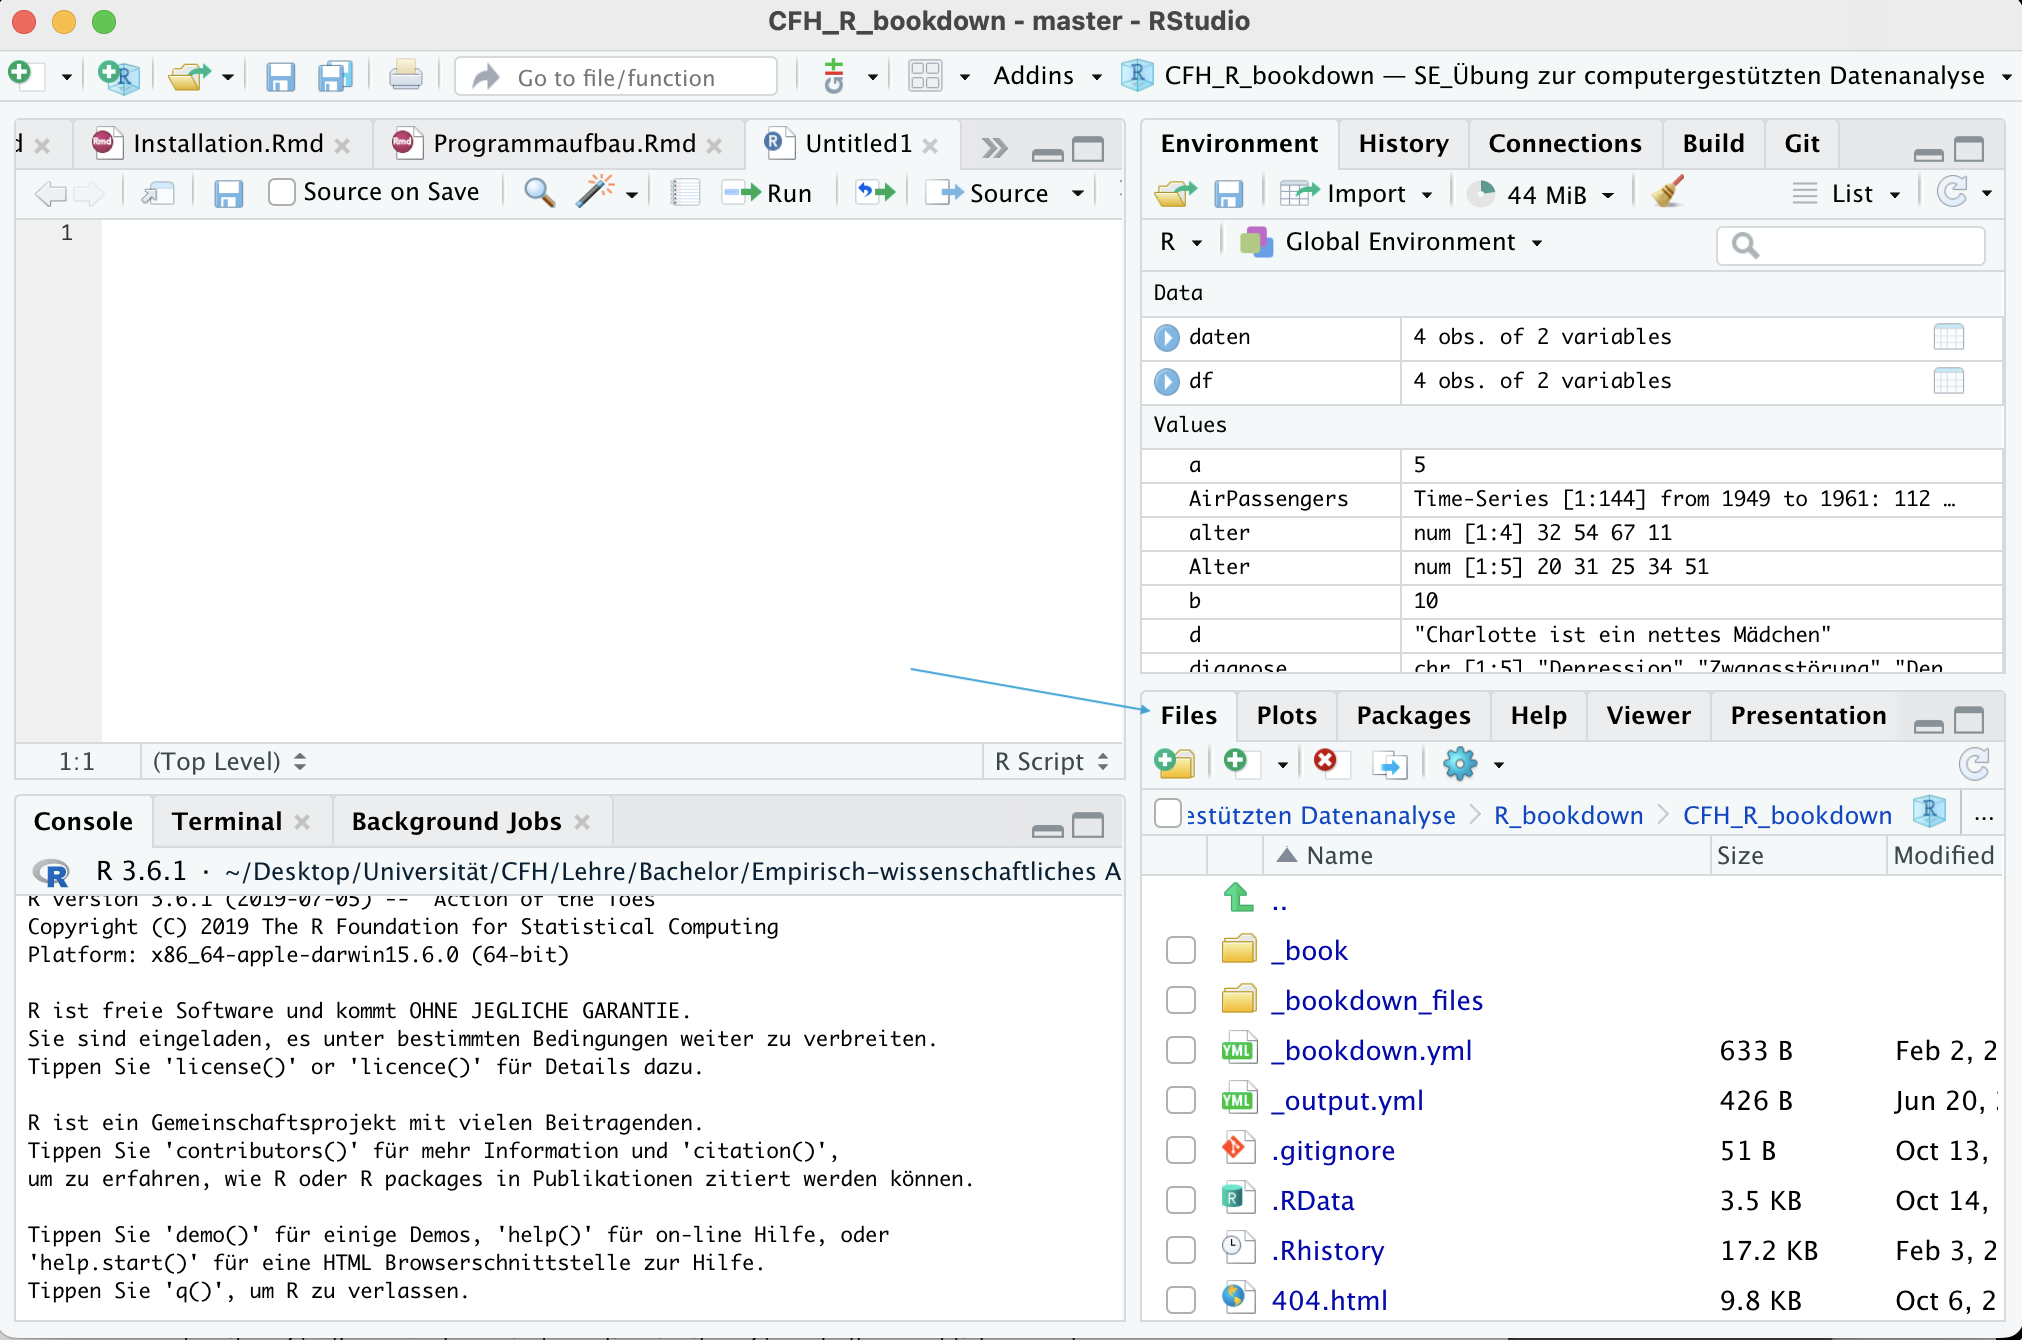
\includegraphics[width=28.08in]{images/windows_files} \caption{Die vier RStudio Fenster}\label{fig:unnamed-chunk-6}
\end{figure}

\begin{enumerate}
\def\labelenumi{\arabic{enumi}.}
\item
  Files - Der Tab ``Files'' gibt Ihnen Zugriff auf das Dateiverzeichnis Ihrer Festplatte. Dateien, die Sie in Ihrem R Projekt benutzen, liegen in der Regel in einem von Ihnen definierten Arbeitsverzeichnis. Wir werden in Kürze ausführlicher über Arbeitsverzeichnisse sprechen.
\item
  Plots - Das Plots-Panel zeigt (keine große Überraschung) alle Ihre Plots an.
\item
  Pakete - Zeigt eine Liste aller auf Ihrer Festplatte installierten R-Pakete und gibt an, ob sie derzeit geladen sind oder nicht. Pakete, die in der aktuellen Sitzung geladen sind, sind markiert, während Pakete, die installiert, aber noch nicht geladen sind, nicht markiert sind. Auf die Pakete gehen wir im nächsten Abschnitt näher ein.
\item
  Hilfe - Hilfemenü für R-Funktionen. Sie können entweder den Namen einer Funktion in das Suchfenster eingeben oder den Code \texttt{?function.name} in der Konsole verwenden, um nach einer Funktion mit dem Namen \texttt{function.name} zu suchen:
\end{enumerate}

\begin{Shaded}
\begin{Highlighting}[]
\NormalTok{?hist   }\CommentTok{\# Wie funktioniert die Histogrammfunktion?}
\NormalTok{?t.test }\CommentTok{\# Wie funktioniert der t{-}Test?}
\end{Highlighting}
\end{Shaded}

\hypertarget{r-packages}{%
\section{R Packages}\label{r-packages}}

Wenn Sie R zum ersten Mal herunterladen und installieren, installieren Sie die Base R Software.
Base R enthält die meisten Funktionen, die Sie täglich verwenden werden, wie mean() und hist().
Allerdings werden hier nur Funktionen angezeigt, die von den ursprünglichen Autoren der Sprache R geschrieben wurden.
Wenn Sie auf Daten und Code zugreifen möchten, die von anderen Personen geschrieben wurden, müssen Sie diese als ``Package'' installieren.
Ein R-Package ist einfach ein Bündel von Funktionen (also bereits geschriebener Code), die in einem übersichtlichen Paket gespeichert sind.

Ein Paket ist wie eine Glühbirne. Um es nutzen zu können, müssen Sie es zunächst in Ihr Haus (d.h. auf Ihren Computer) bestellen, indem Sie es installieren. Wenn Sie ein Paket einmal installiert haben, brauchen Sie es nie wieder zu installieren. Jedes Mal, wenn Sie das Paket tatsächlich verwenden wollen, müssen Sie es jedoch einschalten, indem Sie es laden. Und so geht's:

\hypertarget{r-packages-installieren}{%
\subsection{R Packages installieren}\label{r-packages-installieren}}

Ein Paket zu installieren bedeutet einfach, den Paketcode auf Ihren Computer herunterzuladen. Die gängigste Methode ist das Herunterladen aus dem Comprehensive R Archive Network (CRAN).

Um ein neues R-Paket von CRAN zu installieren, können Sie einfach den Code install.packages(``name'') ausführen, wobei ``name'' der Name des Pakets ist.

Um zum Beispiel das Paket ggplot2 herunterzuladen, welches wir oft zum Erstellen von Graphen verwenden, geben Sie ein:

\begin{Shaded}
\begin{Highlighting}[]
\CommentTok{\# install.packages("ggplot2")}
\end{Highlighting}
\end{Shaded}

\hypertarget{r-packages-laden}{%
\subsection{R Packages laden}\label{r-packages-laden}}

Sobald Sie ein Paket installiert haben, befindet es sich auf Ihrem Computer. Aber nur weil es auf Ihrem Computer ist, bedeutet das nicht, dass R bereit ist, es zu benutzen. Wenn Sie etwas wie eine Funktion oder einen Datensatz aus einem Paket verwenden wollen, müssen Sie \emph{immer} zuerst das Paket in Ihrer R-Sitzung \emph{laden}. Genau wie bei einer Glühbirne müssen Sie sie einschalten, um sie zu benutzen!

Um ein Paket zu laden, verwenden Sie die Funktion \texttt{library()}. Nachdem wir zum Beispiel das Paket \texttt{ggplot2} installiert haben, können wir es mit \texttt{library("ggplot2")} laden:

\begin{Shaded}
\begin{Highlighting}[]
\CommentTok{\#   Laden des "ggplot2" Pakekts, damit wir es benutzen können!}
\CommentTok{\#   Pakete müssen zu Beginn jeder R Session neu geladen werden!}
\FunctionTok{library}\NormalTok{(}\StringTok{"ggplot2"}\NormalTok{)}
\end{Highlighting}
\end{Shaded}

Jetzt, wo Sie das Paket \texttt{ggplot2} geladen haben, können Sie jede seiner Funktionen benutzen (hier die Funktion \texttt{ggplot}, um einen Graph zu erstellen)!

\begin{Shaded}
\begin{Highlighting}[]
\FunctionTok{ggplot}\NormalTok{(}\AttributeTok{data =}\NormalTok{ iris, }\FunctionTok{aes}\NormalTok{(}\AttributeTok{x =}\NormalTok{ Sepal.Length)) }\SpecialCharTok{+} 
  \FunctionTok{geom\_histogram}\NormalTok{()}
\end{Highlighting}
\end{Shaded}

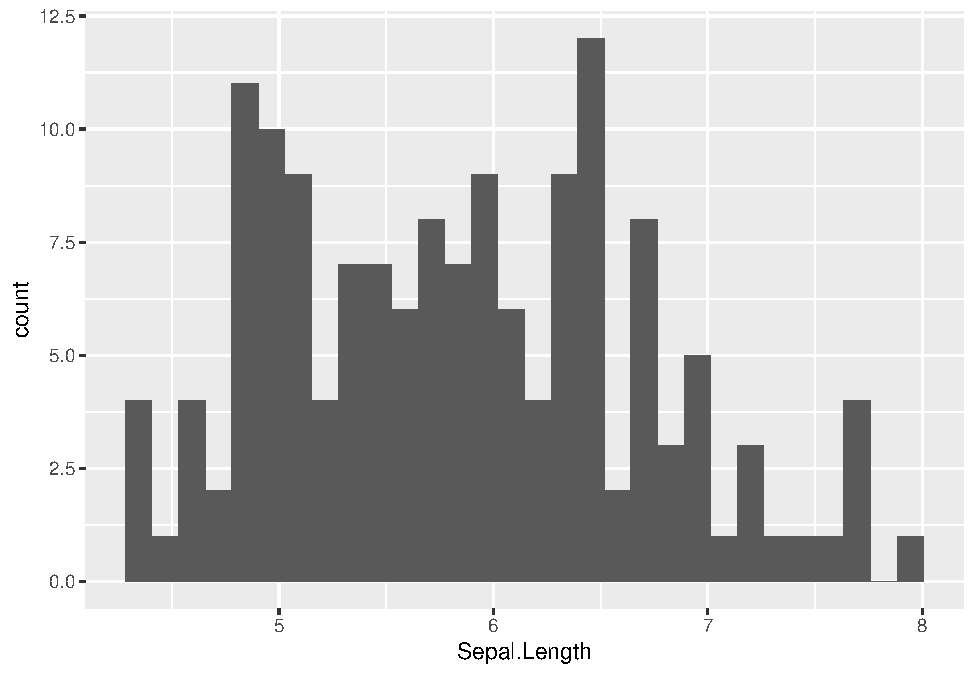
\includegraphics{CFH_R_bookdown_files/figure-latex/unnamed-chunk-10-1.pdf}

Pakete müssen zu Beginn jeder R Session neu geladen werden. Deswegen schreiben wir in der Regel ganz an den Anfang unseres Skripts gleich mehrere Zeilen, mit \texttt{library()} Befehlen für alle R Pakete, die wir für unsere Analyse benötigen werden.

In R gibt es eine Möglichkeit, ein Paket vorübergehend zu laden, ohne die Funktion \texttt{library()} zu verwenden. Um dies zu tun, können Sie einfach die Notation \texttt{package::funktion} verwenden. Diese Notation sagt R einfach, dass es das Paket nur für diesen einen Codeabschnitt laden soll. Zum Beispiel könnte ich die Funktion \texttt{ggplot} aus dem Paket \texttt{ggplot2} wie folgt verwenden:

\begin{Shaded}
\begin{Highlighting}[]
\NormalTok{ggplot2}\SpecialCharTok{::}\FunctionTok{ggplot}\NormalTok{(}\AttributeTok{data =}\NormalTok{ iris, }\FunctionTok{aes}\NormalTok{(}\AttributeTok{x =}\NormalTok{ Sepal.Length)) }\SpecialCharTok{+} 
  \FunctionTok{geom\_histogram}\NormalTok{()}
\end{Highlighting}
\end{Shaded}

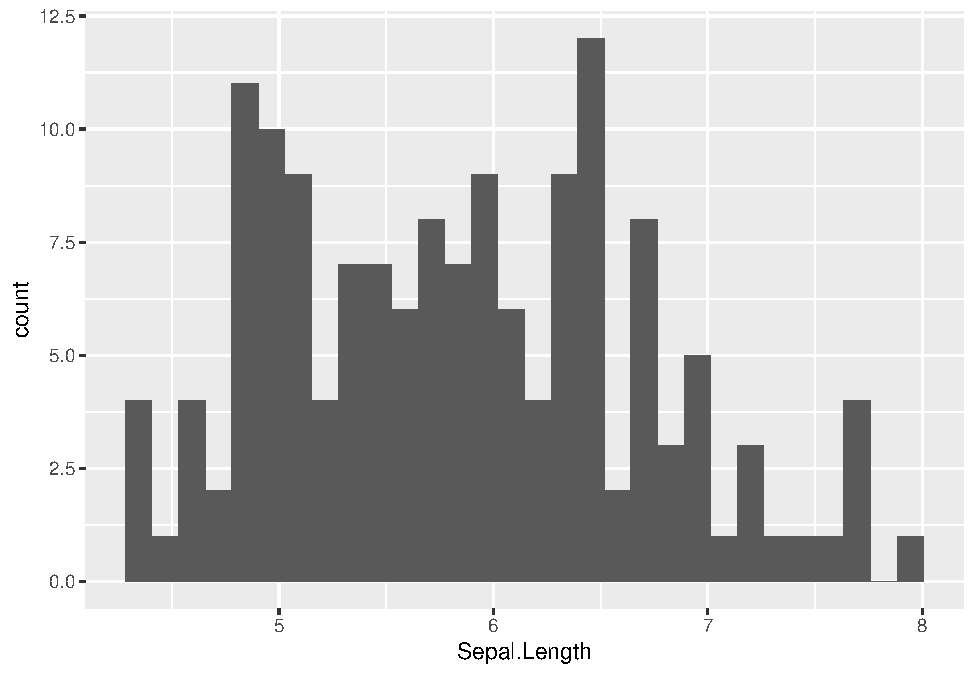
\includegraphics{CFH_R_bookdown_files/figure-latex/unnamed-chunk-11-1.pdf}

Ein Vorteil der Notation ``package::function'' ist, dass für jeden, der den Code liest, sofort klar ist, welches Paket die Funktion enthält. Ein Nachteil ist jedoch, dass Sie, wenn Sie eine Funktion aus einem Paket häufig verwenden, gezwungen sind, den Paketnamen ständig neu einzugeben. Sie können jede Methode verwenden, die für Sie sinnvoll ist.

\hypertarget{datenformate}{%
\chapter{Datenformate}\label{datenformate}}

\begin{figure}
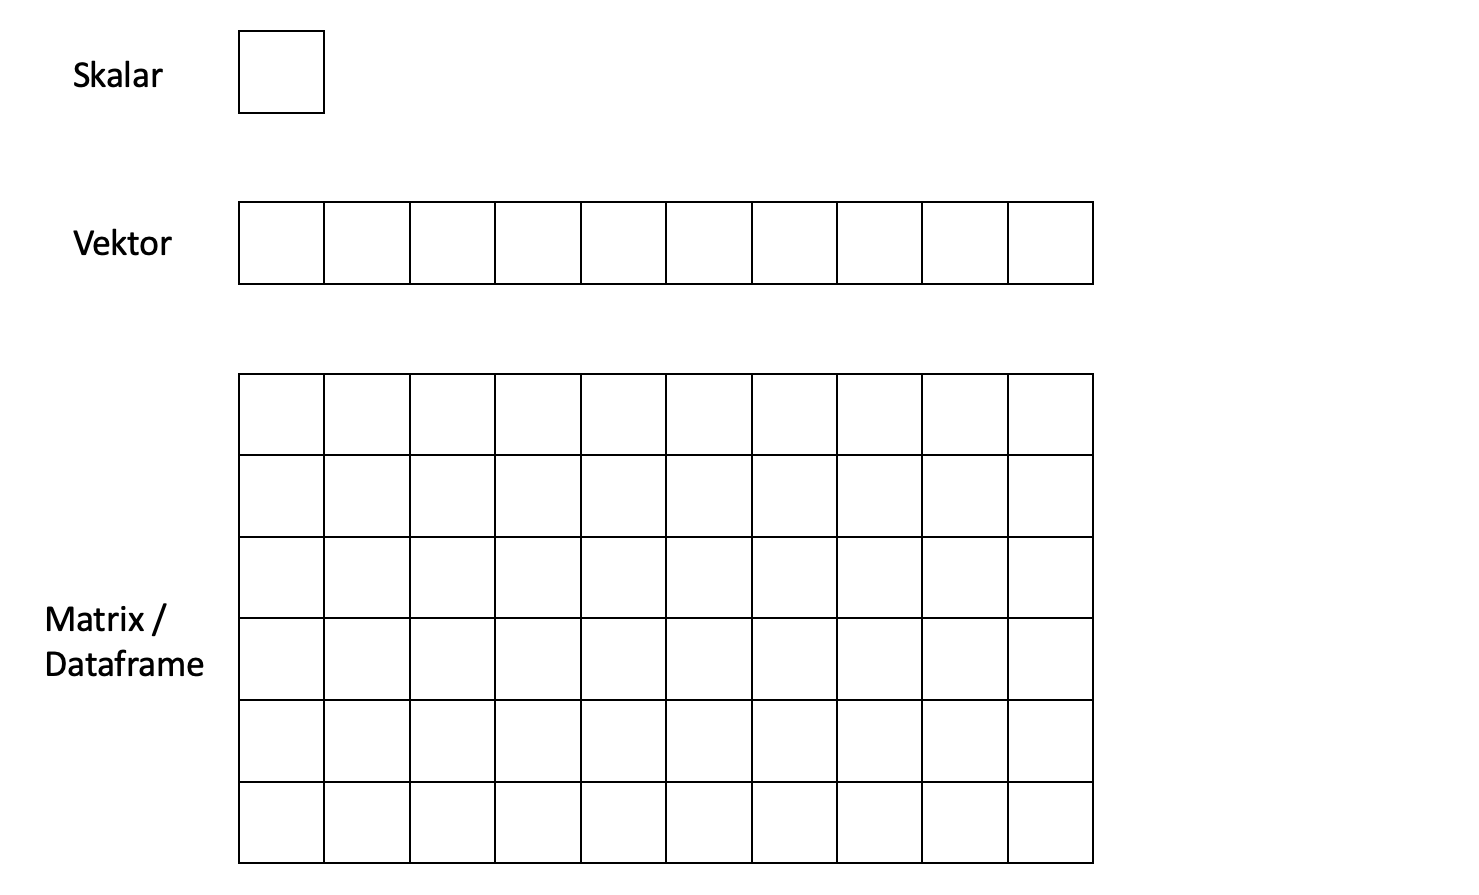
\includegraphics[width=20.54in]{images/Datenformat_1} \caption{Skalar, Vektor, Matrix}\label{fig:unnamed-chunk-12}
\end{figure}

\hypertarget{skalar}{%
\section{Skalar}\label{skalar}}

Der einfachste Objekttyp in R ist der \textbf{Skalar}. Ein Skalar Objekt ist einfach nur ein einzelner Wert, z.B. eine Zahl oder ein Wort.

Hier sind einige Beispiele für numerische Skalar Objekte:

\begin{Shaded}
\begin{Highlighting}[]
\CommentTok{\# Examples of numeric scalars}
\NormalTok{a }\OtherTok{\textless{}{-}} \DecValTok{100}
\NormalTok{b }\OtherTok{\textless{}{-}} \DecValTok{3} \SpecialCharTok{/} \DecValTok{100}
\NormalTok{c }\OtherTok{\textless{}{-}}\NormalTok{ (a }\SpecialCharTok{+}\NormalTok{ b) }\SpecialCharTok{/}\NormalTok{ b}
\end{Highlighting}
\end{Shaded}

Skalare müssen nicht numerisch sein, sondern können auch Worte beinhalten. Wortobjekte heißen in R \textbf{characters} (engl. strings). In R schreibt man Worte immer in Anführungszeichen \texttt{""}. Hier sind einige Beispiele für character Skalare:

\begin{Shaded}
\begin{Highlighting}[]
\CommentTok{\# Beispiele für character Skalare}
\NormalTok{d }\OtherTok{\textless{}{-}} \StringTok{"Psychologe"}
\NormalTok{e }\OtherTok{\textless{}{-}} \StringTok{"Zigarre"}
\NormalTok{f }\OtherTok{\textless{}{-}} \StringTok{"Haben Psychologen wirklich alle Bärte und rauchen Zigarre?"}
\end{Highlighting}
\end{Shaded}

Wie Sie sich vermutlich vorstellen können, behandelt R numerische und character Skalare unterschiedlich. Zum Beispiel lassen sich mit numerischen Skalaren grundlegende arithmetische Operationen durchführen (Addition, Subtraktion, Multiplikation\ldots) -- das funktioniert mit character Skalaren nicht.
Wenn Sie dennoch probieren numerische Operationen auf character Skalare anzuwenden, bekommen Sie eine Fehlermeldung, so wie diese:

\begin{Shaded}
\begin{Highlighting}[]
\NormalTok{a }\OtherTok{=} \StringTok{"1"}
\NormalTok{b }\OtherTok{=} \StringTok{"2"}
\NormalTok{a }\SpecialCharTok{+}\NormalTok{ b}
\end{Highlighting}
\end{Shaded}

\emph{``Fehler in a + b : nicht-numerisches Argument für binären Operator''}

\hypertarget{vektor}{%
\section{Vektor}\label{vektor}}

Machen wir weiter mit \texttt{Vektoren}. Ein Vektor Objekt ist einfach eine Kombination mehrerer Skalare in einem einzelnen Objekt (z.B. eine Zahlen- oder Wortreihe).
Zum Beispiel könnten die Zahlen von 1-10 in einen Vektor mit der Länge 10 kombiniert werden. Oder die Buchstaben des Alphabets könnten in einen Vektor mit der Länge 26 gespeichert werden. Genau wie Skalare, können Vektoren numerisch oder characters sein (Aber nicht beides auf einmal!)

Die einfachste Art einen Vektor zu erstellen ist mit der \texttt{c()} Funktion. Das c steht für ``concatenate'', was auf Englisch so viel heißt wie ``zusammenbringen''. Die \texttt{c()} Funktion nimmt mehrere Skalare als Input und erstellt einen Vektor, der diese Objekte enthält.

Wenn man\texttt{c()} benutzt, muss man immer ein \textbf{Komma} zwischen die Objekte setzen (Skalare oder Vektoren), die man kombinieren möchte.

Lassen Sie uns die \texttt{c()} Funktion nutzen um einen Vektor zu erstellen der \texttt{a} heißt und die Zahlen von 1 bis 7 enthält

\begin{Shaded}
\begin{Highlighting}[]
\NormalTok{a }\OtherTok{=} \FunctionTok{c}\NormalTok{(}\DecValTok{1}\NormalTok{, }\DecValTok{2}\NormalTok{, }\DecValTok{3}\NormalTok{, }\DecValTok{4}\NormalTok{, }\DecValTok{5}\NormalTok{, }\DecValTok{6}\NormalTok{, }\DecValTok{7}\NormalTok{)}
\CommentTok{\# Das Ergebnis ausgeben}
\NormalTok{a}
\end{Highlighting}
\end{Shaded}

\begin{verbatim}
## [1] 1 2 3 4 5 6 7
\end{verbatim}

Sie können auch character Vektoren erstellen, indem Sie die \texttt{c()} auf einzelne character Skalare Funktion anwenden:

\begin{Shaded}
\begin{Highlighting}[]
\NormalTok{char.vec }\OtherTok{=} \FunctionTok{c}\NormalTok{(}\StringTok{"Freud"}\NormalTok{, }\StringTok{"Wundt"}\NormalTok{, }\StringTok{"Bandura"}\NormalTok{, }\StringTok{"Watson"}\NormalTok{, }\StringTok{"Jung"}\NormalTok{)}
\CommentTok{\# Das Ergebnis ausgeben}
\NormalTok{char.vec}
\end{Highlighting}
\end{Shaded}

\begin{verbatim}
## [1] "Freud"   "Wundt"   "Bandura" "Watson"  "Jung"
\end{verbatim}

\hypertarget{vektor-typen}{%
\subsection{Vektor Typen}\label{vektor-typen}}

Vektoren sind ein zentrales Element von R. Ein Vektor kann Zahlen, Buchstaben oder logische Werte enthalten, aber niemals eine Kombination

Der Vektor ist die Entsprechung der \textbf{Variable} und die Skalare, aus denen der Vektor besteht, sind die \textbf{Merkmalsausprägungen} der Variable.

\hypertarget{faktor-variablen}{%
\subsection{Faktor Variablen}\label{faktor-variablen}}

Wir haben bereits gelernt, wie man einen Vektor aus character Objekten erstellt. Manchmal brauchen wir in R jedoch Variablen, die nicht nur Worte enthalten, sondern dem Programm mitteilen, dass es sich um feste Gruppen oder \textbf{Kategorien} handelt. Es geht also nicht nur um eine ``Sammlung'' von Worten (z.B. Nachnamen von Probanden), sondern um festgelegte Analyseeinheiten. Solche Variablen heißen in R \texttt{factor}.

In einer factor Variable ist jeder Kategorie eine Zahl zugeordnet (z.B. 1 = männlich, 2 = weiblich).

Um Faktor Variablen zu erstellen, machen wie einen Vorgang, den man \textbf{Kodieren} nennt und das geht so:

Wir haben einen Vektor mit Codes 1 und 2 für männlich und weiblich vorliegen:

\begin{Shaded}
\begin{Highlighting}[]
\NormalTok{geschlecht }\OtherTok{=} \FunctionTok{c}\NormalTok{(}\DecValTok{1}\NormalTok{, }\DecValTok{2}\NormalTok{, }\DecValTok{2}\NormalTok{, }\DecValTok{1}\NormalTok{, }\DecValTok{2}\NormalTok{)}
\CommentTok{\# Das Ergebnis ausgeben}
\NormalTok{geschlecht}
\end{Highlighting}
\end{Shaded}

\begin{verbatim}
## [1] 1 2 2 1 2
\end{verbatim}

In dieser Form erkennt R diesen Vektor als numerische Variable. Um Sie in einen Faktor umzuwandeln, definieren wir die Zahlen (1 und 2) als \texttt{levels} des Faktors und geben dann jedem level einen Namen (\texttt{labels}):

\begin{Shaded}
\begin{Highlighting}[]
\NormalTok{geschlecht }\OtherTok{=} \FunctionTok{factor}\NormalTok{(geschlecht, }\AttributeTok{levels =} \FunctionTok{c}\NormalTok{(}\DecValTok{1}\NormalTok{,}\DecValTok{2}\NormalTok{), }\AttributeTok{labels =} \FunctionTok{c}\NormalTok{(}\StringTok{"männlich"}\NormalTok{, }\StringTok{"weiblich"}\NormalTok{))}
\CommentTok{\# Das Ergebnis ausgeben}
\NormalTok{geschlecht}
\end{Highlighting}
\end{Shaded}

\begin{verbatim}
## [1] männlich weiblich weiblich männlich weiblich
## Levels: männlich weiblich
\end{verbatim}

Das Ergebnis ist eine codierte Faktorvariable. Wenn wir Sie uns ausgeben lassen erhalten wir unter den Merkmalsausprägungen eine Liste mit den einzelnen Kategorien (levels) des Faktors.

R wird uns für Faktoren alle Ergebnisse nach der \textbf{Reihenfolge} der levels anzeigen. Wenn wir keine Faktorvariable haben, sondern eine character Variable funktioniert die Reihenfolge immer alphabetisch.

\hypertarget{vektor-indizierung}{%
\subsection{Vektor Indizierung}\label{vektor-indizierung}}

Manchmal möchten wir wieder einen einzelnen Skalar auswählen, der als Teil von einem Vektor gespeichert ist. Diese \textbf{Auswahl} eines Einzelelements nennt man \textbf{Indizierung}. Die Auswahl eines kleineren Objekts aus einem größeren Objekt funktioniert in R immer mit \texttt{{[}{]}}.

Benötigen wir aus einem Vektor z.B. genau den 3. Skalar, schreiben wir einfach eine 3 in eckige Klammern hinter den Vektor.

\begin{Shaded}
\begin{Highlighting}[]
\NormalTok{char.vec }\OtherTok{=} \FunctionTok{c}\NormalTok{(}\StringTok{"Freud"}\NormalTok{, }\StringTok{"Wundt"}\NormalTok{, }\StringTok{"Bandura"}\NormalTok{, }\StringTok{"Watson"}\NormalTok{, }\StringTok{"Jung"}\NormalTok{)}
\CommentTok{\# Das Ergebnis ausgeben}
\NormalTok{char.vec[}\DecValTok{5}\NormalTok{]}
\end{Highlighting}
\end{Shaded}

\begin{verbatim}
## [1] "Jung"
\end{verbatim}

\hypertarget{matrizen-und-data.frames}{%
\section{Matrizen und data.frames}\label{matrizen-und-data.frames}}

In der Psychologie beobachten wir für unsere Studien fast immer mehr als eine Variable. Wir könnten diese alle in einzelnen Vektoren speichern und uns die Objektnamen merken. Z.B.

\begin{Shaded}
\begin{Highlighting}[]
\NormalTok{Name }\OtherTok{=} \FunctionTok{c}\NormalTok{(}\StringTok{"Max"}\NormalTok{, }\StringTok{"Maja"}\NormalTok{, }\StringTok{"Mia"}\NormalTok{, }\StringTok{"Moritz"}\NormalTok{, }\StringTok{"Markus"}\NormalTok{)}
\NormalTok{Alter }\OtherTok{=} \FunctionTok{c}\NormalTok{(}\DecValTok{20}\NormalTok{, }\DecValTok{31}\NormalTok{, }\DecValTok{25}\NormalTok{, }\DecValTok{34}\NormalTok{, }\DecValTok{51}\NormalTok{)}
\NormalTok{Diagnose }\OtherTok{=} \FunctionTok{c}\NormalTok{(}\StringTok{"Depression"}\NormalTok{, }\StringTok{"Zwangsstörung"}\NormalTok{, }\StringTok{"Depression"}\NormalTok{, }\StringTok{"Soziale Phobie"}\NormalTok{, }\StringTok{"Depression"}\NormalTok{)}
\end{Highlighting}
\end{Shaded}

\hypertarget{erstellen-von-datenmatrizen}{%
\subsection{Erstellen von Datenmatrizen}\label{erstellen-von-datenmatrizen}}

Praktischer ist es, die einzelnen Vektoren in Tabellenform zu speichern, der \textbf{Datenmatrix}. In R heißen Datenmatrizen \texttt{data.frame}. Wir können die Vektoren folgendermaßen zu einem data.frame kombinieren:

\begin{Shaded}
\begin{Highlighting}[]
\NormalTok{df }\OtherTok{=} \FunctionTok{data.frame}\NormalTok{(Name, Alter, Diagnose)}
\CommentTok{\# Das Ergebnis ausgeben}
\NormalTok{df}
\end{Highlighting}
\end{Shaded}

\begin{verbatim}
##     Name Alter       Diagnose
## 1    Max    20     Depression
## 2   Maja    31  Zwangsstörung
## 3    Mia    25     Depression
## 4 Moritz    34 Soziale Phobie
## 5 Markus    51     Depression
\end{verbatim}

Wie in jeder Datenmatrix entsprechen die \textbf{Zeilen} den einzelnen Personen (Fällen) und die \textbf{Spalten} den Variablen.

R bezeichnet Zeilen und Spalten als \textbf{rows} und \textbf{columns}. Wollen wir z.B. wissen, wie viele Zeilen der data.frame hat, können wir \texttt{nrow()} benutzen. Für die Anzahl der Spalten nehmen wir \texttt{ncol()}:

\begin{Shaded}
\begin{Highlighting}[]
\FunctionTok{nrow}\NormalTok{(df)}
\end{Highlighting}
\end{Shaded}

\begin{verbatim}
## [1] 5
\end{verbatim}

\begin{Shaded}
\begin{Highlighting}[]
\FunctionTok{ncol}\NormalTok{(df)}
\end{Highlighting}
\end{Shaded}

\begin{verbatim}
## [1] 3
\end{verbatim}

Wenn wir die einzelnen Vektoren nicht bereits vorher definiert haben, können wir auch alles in einem Schritt machen. Das Ergebnis ist das gleiche:

\begin{Shaded}
\begin{Highlighting}[]
\NormalTok{df }\OtherTok{=} \FunctionTok{data.frame}\NormalTok{(}\StringTok{"Name"} \OtherTok{=} \FunctionTok{c}\NormalTok{(}\StringTok{"Max"}\NormalTok{, }\StringTok{"Maja"}\NormalTok{, }\StringTok{"Mia"}\NormalTok{, }\StringTok{"Moritz"}\NormalTok{, }\StringTok{"Markus"}\NormalTok{),}
                \StringTok{"Alter"} \OtherTok{=} \FunctionTok{c}\NormalTok{(}\DecValTok{20}\NormalTok{, }\DecValTok{31}\NormalTok{, }\DecValTok{25}\NormalTok{, }\DecValTok{34}\NormalTok{, }\DecValTok{51}\NormalTok{),}
                \StringTok{"Diagnose"} \OtherTok{=} \FunctionTok{c}\NormalTok{(}\StringTok{"Depression"}\NormalTok{, }\StringTok{"Zwangsstörung"}\NormalTok{, }\StringTok{"Depression"}\NormalTok{, }\StringTok{"Soziale Phobie"}\NormalTok{, }\StringTok{"Depression"}\NormalTok{)}
\NormalTok{                )}
\CommentTok{\# Das Ergebnis ausgeben}
\NormalTok{df}
\end{Highlighting}
\end{Shaded}

\begin{verbatim}
##     Name Alter       Diagnose
## 1    Max    20     Depression
## 2   Maja    31  Zwangsstörung
## 3    Mia    25     Depression
## 4 Moritz    34 Soziale Phobie
## 5 Markus    51     Depression
\end{verbatim}

Wollen wir wieder eine einzelne Variable aus dem Datensatz benutzen, können wir diese über das \texttt{\$} Zeichen anwählen:

\begin{Shaded}
\begin{Highlighting}[]
\NormalTok{df}\SpecialCharTok{$}\NormalTok{Alter}
\end{Highlighting}
\end{Shaded}

\begin{verbatim}
## [1] 20 31 25 34 51
\end{verbatim}

\hypertarget{indizierung}{%
\subsection{Indizierung}\label{indizierung}}

Wollen wir aus dem data.frame wieder einzelne Elemente verwenden, nutzen wir wieder die Indizierung. Auch hier brauchen wir die \texttt{{[}{]}}. Da wir im data.frame Zeilen und Spalten haben, brauchen wir eine Möglichkeit, beides auszuwählen, wie ein Curser der von links nach rechts, bzw. von oben nach unten läuft.

Wir trennen dafür unsere \texttt{{[}{]}} mit einem Komma \texttt{{[},{]}}. Alles, was \textbf{links vom Komma} steht, bezieht sich auf Zeilen alles \textbf{rechts vom Komma} bezieht sich auf Spalten.

Lassen Sie uns einmal die Zelle in der 1. Zeile (also die 1. Person) und der 3. Variable auswählen:

\begin{Shaded}
\begin{Highlighting}[]
\NormalTok{df[}\DecValTok{1}\NormalTok{,}\DecValTok{3}\NormalTok{]}
\end{Highlighting}
\end{Shaded}

\begin{verbatim}
## [1] Depression
## Levels: Depression Soziale Phobie Zwangsstörung
\end{verbatim}

Lassen wir die Zahl vor dem Komma weg, bekommen wir alle Werte aus der Spalte:

\begin{Shaded}
\begin{Highlighting}[]
\NormalTok{df[,}\DecValTok{3}\NormalTok{]}
\end{Highlighting}
\end{Shaded}

\begin{verbatim}
## [1] Depression     Zwangsstörung  Depression     Soziale Phobie Depression    
## Levels: Depression Soziale Phobie Zwangsstörung
\end{verbatim}

Lassen wir die Zahl nach dem Komma weg, bekommen wir alle Werte aus der Reihe:

\begin{Shaded}
\begin{Highlighting}[]
\NormalTok{df[}\DecValTok{1}\NormalTok{,]}
\end{Highlighting}
\end{Shaded}

\begin{verbatim}
##   Name Alter   Diagnose
## 1  Max    20 Depression
\end{verbatim}

\hypertarget{daten-erstellen}{%
\chapter{Daten erstellen}\label{daten-erstellen}}

\hypertarget{manuell}{%
\section{Manuell}\label{manuell}}

Die manuelle Eingabe von Daten erfolgt über die \texttt{c()} Funktion. Mit ihrer Hilfe können wir Skalare zu Vektoren verbinden\ldots{}

\begin{Shaded}
\begin{Highlighting}[]
\NormalTok{a }\OtherTok{=} \FunctionTok{c}\NormalTok{(}\DecValTok{1}\NormalTok{, }\DecValTok{2}\NormalTok{, }\DecValTok{4}\NormalTok{, }\DecValTok{6}\NormalTok{, }\DecValTok{1}\NormalTok{)}
\end{Highlighting}
\end{Shaded}

\ldots mehrere Vektoren aneinanderhängen\ldots{}

\begin{Shaded}
\begin{Highlighting}[]
\NormalTok{a }\OtherTok{=} \FunctionTok{c}\NormalTok{(}\DecValTok{1}\NormalTok{, }\DecValTok{2}\NormalTok{, }\DecValTok{4}\NormalTok{, }\DecValTok{6}\NormalTok{, }\DecValTok{1}\NormalTok{)}
\NormalTok{b }\OtherTok{=} \FunctionTok{c}\NormalTok{(}\DecValTok{2}\NormalTok{, }\DecValTok{3}\NormalTok{)}
\NormalTok{c }\OtherTok{=} \FunctionTok{c}\NormalTok{(a, b)}
\NormalTok{c}
\end{Highlighting}
\end{Shaded}

\begin{verbatim}
## [1] 1 2 4 6 1 2 3
\end{verbatim}

\ldots und Vektoren gleicher Länge zu data.frames kombinieren:

\begin{Shaded}
\begin{Highlighting}[]
\NormalTok{daten }\OtherTok{=} \FunctionTok{data.frame}\NormalTok{(}\AttributeTok{aufmerksamkeit =} \FunctionTok{c}\NormalTok{(}\DecValTok{58}\NormalTok{, }\DecValTok{46}\NormalTok{, }\DecValTok{29}\NormalTok{, }\DecValTok{51}\NormalTok{),}
                   \AttributeTok{gedaechtnis =} \FunctionTok{c}\NormalTok{(}\DecValTok{22}\NormalTok{, }\DecValTok{67}\NormalTok{, }\DecValTok{22}\NormalTok{, }\DecValTok{31}\NormalTok{))}
\NormalTok{daten}
\end{Highlighting}
\end{Shaded}

\begin{verbatim}
##   aufmerksamkeit gedaechtnis
## 1             58          22
## 2             46          67
## 3             29          22
## 4             51          31
\end{verbatim}

\hypertarget{automatisch}{%
\section{Automatisch}\label{automatisch}}

Wir haben bereits die \texttt{c()} Funktion gelernt.

Die \texttt{c()} Funktion ist die einfachste Art einen Vektor zu erstellen, sie ist aber vermutlich auch die umständlichste. Stellen Sie sich zum Beispiel vor, Sie wollen einen Vektor erstellen, der alle Zahlen von 0 bis 100 enthält. Diese Zahlen wollen Sie definitiv nicht alle in die Klammer von \texttt{c()} eintippen.

Glücklicherweise hat R viele eingebaute Funktionen, um leicht automatisch numerische Vektoren zu erstellen.

Lassen Sie uns mit dreien davon starten\texttt{a:b}, \texttt{seq()}, and \texttt{rep()}:

\begin{longtable}[]{@{}
  >{\raggedright\arraybackslash}p{(\columnwidth - 4\tabcolsep) * \real{0.3881}}
  >{\raggedright\arraybackslash}p{(\columnwidth - 4\tabcolsep) * \real{0.4478}}
  >{\raggedright\arraybackslash}p{(\columnwidth - 4\tabcolsep) * \real{0.1642}}@{}}
\toprule()
\begin{minipage}[b]{\linewidth}\raggedright
Funktion
\end{minipage} & \begin{minipage}[b]{\linewidth}\raggedright
Beispiel
\end{minipage} & \begin{minipage}[b]{\linewidth}\raggedright
Ergebnis
\end{minipage} \\
\midrule()
\endhead
\texttt{c(a,\ b,\ ...)} & \texttt{c(1,\ 5,\ 9)} & 1, 5, 9 \\
\texttt{a:b} & \texttt{1:5} & 1, 2, 3, 4, 5 \\
\texttt{seq(from,\ to,\ by,\ length.out)} & \texttt{seq(from\ =\ 0,\ to\ =\ 6,\ by\ =\ 2)} & 0, 2, 4, 6 \\
\texttt{rep(x,\ times,\ each,\ length.out)} & \texttt{rep(c(7,\ 8),\ times\ =\ 2,\ each\ =\ 2)} & 7, 7, 8, 8, 7, 7, 8, 8 \\
\bottomrule()
\end{longtable}

\hypertarget{zufuxe4llig}{%
\section{Zufällig}\label{zufuxe4llig}}

In R kann man Daten anhand einer Wahrscheinlichkeitsverteilung simulieren.

Wollen wir z.B. eine normalverteilte Variable mit zufälligen Werten erstellen, können wir die \texttt{rnorm()} Funktion nutzen.

Dafür müssen wir lediglich angeben, wie viele Werte wir haben wollen (\texttt{n}) und welchen Mittelwert (\texttt{mean}) und welche Standardabweichung (\texttt{sd}) die Verteilung haben soll:

\begin{Shaded}
\begin{Highlighting}[]
\FunctionTok{rnorm}\NormalTok{(}\AttributeTok{n =} \DecValTok{20}\NormalTok{, }\AttributeTok{mean =} \DecValTok{0}\NormalTok{, }\AttributeTok{sd =} \DecValTok{1}\NormalTok{)}
\end{Highlighting}
\end{Shaded}

\begin{verbatim}
##  [1] -0.124675547  0.923934684  1.036799704  0.159599728  1.123417617
##  [6]  0.026977181  0.003212397 -0.334274578 -1.678625666  0.658952124
## [11] -1.233806055  0.174593319  0.230391396  0.004262633 -1.310425214
## [16] -0.056179427 -0.275926178 -0.171228615 -1.495094148 -0.935589983
\end{verbatim}

\hypertarget{daten-importieren-und-speichern}{%
\chapter{Daten importieren und speichern}\label{daten-importieren-und-speichern}}

In diesem Kapitel werden wir die Grundlagen der R-Objektverwaltung behandeln. Es wird erläutert, wie Sie neue Objekte, z. B. externe Datensätze, in R laden, wie Sie die bereits vorhandenen Objekte verwalten und wie Sie Objekte aus R in externe Dateien exportieren, die Sie mit anderen Personen teilen oder für Ihre eigene zukünftige Verwendung speichern können.

\hypertarget{funktionen-zur-organisation-des-workspace}{%
\section{Funktionen zur Organisation des Workspace}\label{funktionen-zur-organisation-des-workspace}}

In diesem Kapitel werden wir einige hilfreiche Funktionen zur Verwaltung Ihres Arbeitsbereichs vorstellen:

\begin{longtable}[]{@{}
  >{\raggedright\arraybackslash}p{(\columnwidth - 2\tabcolsep) * \real{0.4167}}
  >{\raggedright\arraybackslash}p{(\columnwidth - 2\tabcolsep) * \real{0.5833}}@{}}
\toprule()
\begin{minipage}[b]{\linewidth}\raggedright
Code
\end{minipage} & \begin{minipage}[b]{\linewidth}\raggedright
Description
\end{minipage} \\
\midrule()
\endhead
\texttt{ls()} & Alle Objekte im aktuellen Arbeitsbereich anzeigen \\
\texttt{rm(x,\ y,\ ..)} & Entfernt die Objete \texttt{y}, \texttt{y}\ldots{} aus dem Arbeitsbereich \\
\texttt{rm(list\ =\ ls())} & Entfernt \emph{alle} Objekte aus dem Arbeitsbereich \\
\texttt{getwd()} & Zeigt das aktuelle Arbeitsverzeichnis an \\
\texttt{setwd(file\ =\ "dir)} & Wechselt das Arbeitsverzeichnis zu einem bestimmten Dateipfad \\
\texttt{list.files()} & Zeigt die Namen aller Dateien im Arbeitsverzeichnis an \\
\texttt{write.table(x,\ file\ =\ "mydata.txt",\ sep)} & speichert das Objekt \texttt{x} als Textdatei \texttt{mydata.txt}. Definiere die Trennung der Spalten mittels \texttt{sep} (z.B.; \texttt{sep\ =\ ","} für eine kommagetrennte Datei (csv) und \texttt{sep\ =\ \textbackslash{}t"} für eine tab-getrennte Datei). \\
\texttt{write\_rds(x,"meineDaten.rds)} & Speichert Objekt x in das R Objekt \texttt{meineDaten.rds} \\
\texttt{save.image(file\ =\ "meineSession.RData")} & Speichert \emph{alle} Objekte aus dem Arbeitsbereich nach \texttt{meineSession.RData} \\
\texttt{read\_rds}(``Daten.rds'')\texttt{\textbar{}Läd\ das\ rds\ Objekt}Daten.rds\texttt{\textbar{}\ \textbar{}}read.csv\texttt{("Daten.csv")} & Läd den csv Datensatz \texttt{Daten.csv} \\
\texttt{foreign::read.spss("Daten.sav")} & Läd den SPSS Datensatz \texttt{Daten.sav} \\
\texttt{read.csv("Daten.csv")} & Läd den csv Datensatz \texttt{Daten.csv} \\
\texttt{readxl::read\_xlsx("Daten.xlsx")} & Läd den Excel Datensatz \texttt{Daten.xlsx} \\
\bottomrule()
\end{longtable}

Ihr Computer ist ein Labyrinth aus Ordnern und Dateien. Wenn Sie außerhalb von R eine bestimmte Datei öffnen möchten, öffnen Sie wahrscheinlich ein Explorer-Fenster, mit dem Sie die Ordner auf Ihrem Computer visuell durchsuchen können. Oder Sie wählen die zuletzt geöffneten Dateien aus oder geben den Namen der Datei in ein Suchfeld ein, um den Computer die Suche für Sie übernehmen zu lassen. Während dieses Vorgehen normalerweise für nicht-programmierende Aufgaben funktioniert, ist es für R ein No-Go. Das Hauptproblem ist, dass Sie bei all diesen Methoden Ihre Ordner visuell durchsuchen und die Maus bewegen müssen, um Ordner und Dateien auszuwählen, die dem Gesuchten entsprechen. Wenn Sie in R programmieren, müssen Sie alle Schritte in Ihren Analysen so spezifizieren, dass sie von anderen und von Ihnen selbst leicht nachvollzogen werden können. Das bedeutet, dass Sie nicht einfach sagen können: ``Finde diese eine Datei, die ich mir vor einer Woche gemailt habe'' oder ``Suche nach einer Datei, die so aussieht wie''MeinFoto.jpg''. Stattdessen müssen Sie in der Lage sein, R-Code zu schreiben, der R genau sagt, wo wichtige Dateien zu finden sind - entweder auf Ihrem Computer oder im Internet.

Um diese Aufgabe zu erleichtern, verwendet R Arbeitsverzeichnisse.

\hypertarget{arbeitsverzeichnis-working-directory}{%
\section{Arbeitsverzeichnis (Working Directory)}\label{arbeitsverzeichnis-working-directory}}

Das Arbeitsverzeichnis ist lediglich ein Dateipfad auf Ihrem Computer, der den Standardspeicherort aller Dateien festlegt, die Sie in R einlesen oder aus R heraus speichern. Mit anderen Worten, ein Arbeitsverzeichnis ist wie eine kleine Kiste irgendwo auf Ihrem Computer, die an ein bestimmtes Analyseprojekt gebunden ist. Wenn Sie R auffordern, einen Datensatz zu importieren wird davon ausgegangen, dass sich die Datei in Ihrem Arbeitsverzeichnis befindet.

Sie können zu jedem Zeitpunkt nur ein Arbeitsverzeichnis aktiv haben. Das aktive Arbeitsverzeichnis wird als Ihr aktuelles Arbeitsverzeichnis bezeichnet.

\hypertarget{working-environment}{%
\section{Working Environment}\label{working-environment}}

Der Arbeitsbereich (auch als Arbeitsumgebung bezeichnet) enthält alle Objekte und Funktionen, die Sie entweder in der aktuellen Sitzung definiert oder aus einer früheren Sitzung geladen haben. Als Sie RStudio zum ersten Mal starteten, war die Arbeitsumgebung leer, da Sie keine neuen Objekte oder Funktionen erstellt hatten. Wenn Sie jedoch neue Objekte und Funktionen mit dem Zuweisungsoperator = definiert haben, wurden diese neuen Objekte in Ihrer Arbeitsumgebung gespeichert. Wenn Sie RStudio nach der Definition neuer Objekte schlossen, erhielten Sie wahrscheinlich eine Meldung mit der Frage ``Save workspace image\ldots?''. Damit möchte RStudio Sie fragen, ob Sie alle derzeit in Ihrem Arbeitsbereich definierten Objekte als Bilddatei auf Ihrem Computer speichern möchten.

\begin{Shaded}
\begin{Highlighting}[]
\CommentTok{\# getwd()}
\end{Highlighting}
\end{Shaded}

\hypertarget{daten-importieren}{%
\section{Daten importieren}\label{daten-importieren}}

Wenn Sie Daten in Ihrem Arbeitsverzeichnis haben, können Sie diese nun in R einlesen und dort mit ihnen rechnen. Nehmen wir an, Sie haben in Ihrem Arbeitsverzeichnis einen Ordner mit dem Namen \texttt{data}.

Je nachdem in welchem Format die Daten vorliegen, muss ein eigener Befehl genutzt werden. Teilweise braucht man hier auch eigene Pakete (z.B. Excel- oder SPSS-Format).

\hypertarget{rds-format}{%
\subsection{rds-Format}\label{rds-format}}

.rds ist das R-eigene Format. Es speichert alle Objekte die es in R gibt, also potentiell nicht nur Datensätze, sondern auch Testergebnisse, Bilder, o.ä. mittels der Funktion \texttt{read\_rds()} können wir die Objekte einlesen. Dafür müssen wir das Paket \texttt{readr} installiert und mittels \texttt{library} eingelesen haben.

\begin{Shaded}
\begin{Highlighting}[]
\NormalTok{data }\OtherTok{=} \FunctionTok{load}\NormalTok{(}\AttributeTok{file =} \StringTok{"data/personality.RData"}\NormalTok{)}

\CommentTok{\# erste Zeilen des Datensatzes ansehen}
\FunctionTok{head}\NormalTok{(data)}
\end{Highlighting}
\end{Shaded}

\begin{verbatim}
## [1] "data"
\end{verbatim}

\hypertarget{csv-format}{%
\subsection{csv-Format}\label{csv-format}}

Das .csv Format (comma-separated-values) ist eines der gängigsten in der Statistik. Es lässt sich mit allen gebräuchlichen Tabellenprogrammen öffnen (also neben R auch mit Excel, Numbers, o.ä.).

Um einen .csv Datensatz einzulesen, speichern wir ihn mittel \texttt{read.csv()} in ein von uns benanntes Objekt. Dieses können wir nennen wie wir wollen, z.B. \texttt{data} (schön kurz):

\begin{Shaded}
\begin{Highlighting}[]
\NormalTok{data }\OtherTok{=} \FunctionTok{read.csv}\NormalTok{(}\StringTok{"data/personality.csv"}\NormalTok{)}

\CommentTok{\# erste Zeilen des Datensatzes ansehen}
\FunctionTok{head}\NormalTok{(data)}
\end{Highlighting}
\end{Shaded}

\begin{verbatim}
##   ID NEO_1_N NEO_2_E NEO_3_O NEO_4_V NEO_5_G NEO_6_N NEO_7_E NEO_8_O NEO_9_V
## 1  1       2       4       0       3       3       0       2       3       0
## 2  2       4       4       0       3       4       0       4       4       0
## 3  3       4       4       2       4       4       0       4       4       0
## 4  4       4       3       4       3       3       0       2       4       0
## 5  5       4       4       1       3       3       0       3       4       4
## 6  6       4       4       0       4       0       1       4       4       0
##   NEO_10_G NEO_11_N NEO_12_E NEO_13_O NEO_14_V NEO_15_G NEO_16_N NEO_17_E
## 1        3        4        1        2        0        4        4        3
## 2        4        1        0        3        0        3        4        4
## 3        4        4        2        4        0        0        4        4
## 4        3        0        0        2        0        0        4        4
## 5        3        1        4        4        0        0        4        4
## 6        2        0        0        4        0        0        4        4
##   NEO_18_O NEO_19_V NEO_20_G NEO_21_N NEO_22_E NEO_23_O NEO_24_V NEO_25_G
## 1        4        3        4        0        4        2        2        3
## 2        3        4        4        0        3        4        0        4
## 3        0        4        4        0        4        4        1        4
## 4        0        4        4        4        4        4        0        3
## 5        0        4        1        1        3        4        0        2
## 6        0        4        4        0        3        4        4        4
##   NEO_26_N NEO_27_E NEO_28_O NEO_29_V NEO_30_G NEO_31_N NEO_32_E NEO_33_O
## 1        4        4        4        2        4        3        0        0
## 2        2        0        1        0        4        4        4        4
## 3        4        0        0        0        1        4        4        3
## 4        0        0        0        0        0        4        4        0
## 5        0        4        4        2        4        4        3        4
## 6        0        0        4        2        0        4        3        2
##   NEO_34_V NEO_35_G NEO_36_N NEO_37_E NEO_38_O NEO_39_V NEO_40_G NEO_41_N
## 1        3        4        2        4        1        0        4        4
## 2        4        4        0        4        3        1        4        0
## 3        4        4        3        4        2        0        4        0
## 4        3        4        0        3        3        1        4        0
## 5        3        3        0        4        0        2        3        0
## 6        4        4        0        2        4        2        4        0
##   NEO_42_E NEO_43_O NEO_44_V NEO_45_G NEO_46_N NEO_47_E NEO_48_O NEO_49_V
## 1        2        1        4        0        4        4        3        3
## 2        2        4        0        2        4        0        4        4
## 3        4        4        4        0        4        0        4        4
## 4        2        2        0        0        4        4        3        3
## 5        0        2        0        1        4        0        2        3
## 6        0        4        0        0        4        0        2        4
##   NEO_50_G NEO_51_N NEO_52_E NEO_53_O NEO_54_V NEO_55_G NEO_56_N NEO_57_E
## 1        3        0        4        2        0        0        2        2
## 2        4        0        4        4        0        0        0        0
## 3        4        3        4        4        4        0        0        1
## 4        4        4        4        1        0        0        4        0
## 5        3        0        3        3        0        4        0        1
## 6        4        0        4        4        1        0        0        0
##   NEO_58_O NEO_59_V NEO_60_G
## 1        3        1        4
## 2        3        0        4
## 3        4        0        4
## 4        4        1        3
## 5        3        4        4
## 6        4        0        3
\end{verbatim}

\hypertarget{sav-format}{%
\subsection{sav-Format}\label{sav-format}}

Das .sav Format ist das Format in welchem SPSS Datensätze abgespeichert werden. Dies kommt gerade in den Sozialwissenschaften relativ häufig vor, weshalb wir diese Art von Datein auf jeden Fall einlesen können sollten.

Um einen .sav Datensatz einzulesen, speichern wir ihn mittel \texttt{read.spss()} in ein von uns benanntes Objekt. Dafür müssen wir das Paket \texttt{foreign} installiert und mittels \texttt{library} eingelesen haben. Damit R den Datensatz automatisch in einen data.frame speichert, geben wir als Zusatzoption \texttt{to.data.frame\ =\ TRUE} an:

\begin{Shaded}
\begin{Highlighting}[]
\FunctionTok{library}\NormalTok{(foreign)}
\NormalTok{data }\OtherTok{=} \FunctionTok{read.spss}\NormalTok{(}\StringTok{"data/personality.sav"}\NormalTok{, }\AttributeTok{to.data.frame =} \ConstantTok{TRUE}\NormalTok{)}

\CommentTok{\# erste Zeilen des Datensatzes ansehen}
\FunctionTok{head}\NormalTok{(data)}
\end{Highlighting}
\end{Shaded}

\begin{verbatim}
##   ID NEO_1_N NEO_2_E NEO_3_O NEO_4_V NEO_5_G NEO_6_N NEO_7_E NEO_8_O NEO_9_V
## 1  1       2       4       0       3       3       0       2       3       0
## 2  2       4       4       0       3       4       0       4       4       0
## 3  3       4       4       2       4       4       0       4       4       0
## 4  4       4       3       4       3       3       0       2       4       0
## 5  5       4       4       1       3       3       0       3       4       4
## 6  6       4       4       0       4       0       1       4       4       0
##   NEO_10_G NEO_11_N NEO_12_E NEO_13_O NEO_14_V NEO_15_G NEO_16_N NEO_17_E
## 1        3        4        1        2        0        4        4        3
## 2        4        1        0        3        0        3        4        4
## 3        4        4        2        4        0        0        4        4
## 4        3        0        0        2        0        0        4        4
## 5        3        1        4        4        0        0        4        4
## 6        2        0        0        4        0        0        4        4
##   NEO_18_O NEO_19_V NEO_20_G NEO_21_N NEO_22_E NEO_23_O NEO_24_V NEO_25_G
## 1        4        3        4        0        4        2        2        3
## 2        3        4        4        0        3        4        0        4
## 3        0        4        4        0        4        4        1        4
## 4        0        4        4        4        4        4        0        3
## 5        0        4        1        1        3        4        0        2
## 6        0        4        4        0        3        4        4        4
##   NEO_26_N NEO_27_E NEO_28_O NEO_29_V NEO_30_G NEO_31_N NEO_32_E NEO_33_O
## 1        4        4        4        2        4        3        0        0
## 2        2        0        1        0        4        4        4        4
## 3        4        0        0        0        1        4        4        3
## 4        0        0        0        0        0        4        4        0
## 5        0        4        4        2        4        4        3        4
## 6        0        0        4        2        0        4        3        2
##   NEO_34_V NEO_35_G NEO_36_N NEO_37_E NEO_38_O NEO_39_V NEO_40_G NEO_41_N
## 1        3        4        2        4        1        0        4        4
## 2        4        4        0        4        3        1        4        0
## 3        4        4        3        4        2        0        4        0
## 4        3        4        0        3        3        1        4        0
## 5        3        3        0        4        0        2        3        0
## 6        4        4        0        2        4        2        4        0
##   NEO_42_E NEO_43_O NEO_44_V NEO_45_G NEO_46_N NEO_47_E NEO_48_O NEO_49_V
## 1        2        1        4        0        4        4        3        3
## 2        2        4        0        2        4        0        4        4
## 3        4        4        4        0        4        0        4        4
## 4        2        2        0        0        4        4        3        3
## 5        0        2        0        1        4        0        2        3
## 6        0        4        0        0        4        0        2        4
##   NEO_50_G NEO_51_N NEO_52_E NEO_53_O NEO_54_V NEO_55_G NEO_56_N NEO_57_E
## 1        3        0        4        2        0        0        2        2
## 2        4        0        4        4        0        0        0        0
## 3        4        3        4        4        4        0        0        1
## 4        4        4        4        1        0        0        4        0
## 5        3        0        3        3        0        4        0        1
## 6        4        0        4        4        1        0        0        0
##   NEO_58_O NEO_59_V NEO_60_G
## 1        3        1        4
## 2        3        0        4
## 3        4        0        4
## 4        4        1        3
## 5        3        4        4
## 6        4        0        3
\end{verbatim}

\hypertarget{xlsx-format}{%
\subsection{xlsx-Format}\label{xlsx-format}}

Das .xlsx Format ist das Format in welchem Excel Datensätze abgespeichert werden. Auch das kommt oft vor, da es viele Forscher:innen vorziehen Daten in Excel Tabellen einzutragen.

Um einen .xlsx Datensatz einzulesen, speichern wir ihn mittels \texttt{read\_xlsx()} in ein von uns benanntes Objekt. Dafür müssen wir das Paket \texttt{readxl} installiert und mittels \texttt{library} eingelesen haben. Da in Excel Tabellen manchmal mehrere Arbeitsblätter (engl. ``sheets'') vorliegen, geben wir den Namen des Arbeitsblatt, welches wir brauchen, zusätzlich an:

\begin{Shaded}
\begin{Highlighting}[]
\FunctionTok{library}\NormalTok{(readxl)}
\NormalTok{data }\OtherTok{=} \FunctionTok{read\_xlsx}\NormalTok{(}\StringTok{"data/personality.xlsx"}\NormalTok{, }\AttributeTok{sheet =} \StringTok{"Tabelle1"}\NormalTok{)}

\CommentTok{\# erste Zeilen des Datensatzes ansehen}
\FunctionTok{head}\NormalTok{(data)}
\end{Highlighting}
\end{Shaded}

\begin{verbatim}
## # A tibble: 6 x 61
##      ID NEO_1_N NEO_2_E NEO_3_O NEO_4_V NEO_5_G NEO_6_N NEO_7_E NEO_8_O NEO_9_V
##   <dbl>   <dbl>   <dbl>   <dbl>   <dbl>   <dbl>   <dbl> <chr>     <dbl> <chr>  
## 1     1       2       4       0       3       3       0 2             3 0      
## 2     2       4       4       0       3       4       0 4             4 0      
## 3     3       4       4       2       4       4       0 4             4 0      
## 4     4       4       3       4       3       3       0 2             4 0      
## 5     5       4       4       1       3       3       0 3             4 4      
## 6     6       4       4       0       4       0       1 4             4 0      
## # i 51 more variables: NEO_10_G <dbl>, NEO_11_N <dbl>, NEO_12_E <dbl>,
## #   NEO_13_O <dbl>, NEO_14_V <dbl>, NEO_15_G <dbl>, NEO_16_N <dbl>,
## #   NEO_17_E <dbl>, NEO_18_O <dbl>, NEO_19_V <dbl>, NEO_20_G <dbl>,
## #   NEO_21_N <dbl>, NEO_22_E <dbl>, NEO_23_O <dbl>, NEO_24_V <dbl>,
## #   NEO_25_G <dbl>, NEO_26_N <dbl>, NEO_27_E <dbl>, NEO_28_O <dbl>,
## #   NEO_29_V <dbl>, NEO_30_G <dbl>, NEO_31_N <dbl>, NEO_32_E <dbl>,
## #   NEO_33_O <dbl>, NEO_34_V <dbl>, NEO_35_G <dbl>, NEO_36_N <dbl>, ...
\end{verbatim}

\hypertarget{daten-speichern}{%
\section{Daten speichern}\label{daten-speichern}}

In alle vorgestellten Formate können wir unsere Daten natürlich auch abspeichern. Erstellen wir dafür einen schnellen Test-Datensatz mittels \texttt{data.frame}:

\begin{Shaded}
\begin{Highlighting}[]
\NormalTok{newdata }\OtherTok{=} \FunctionTok{data.frame}\NormalTok{(}\AttributeTok{Variable1 =} \FunctionTok{c}\NormalTok{(}\DecValTok{1}\NormalTok{, }\DecValTok{2}\NormalTok{, }\DecValTok{3}\NormalTok{, }\DecValTok{4}\NormalTok{),}
                     \AttributeTok{Variable2 =} \FunctionTok{c}\NormalTok{(}\StringTok{"Person1"}\NormalTok{, }\StringTok{"Person2"}\NormalTok{, }\StringTok{"Person3"}\NormalTok{, }\StringTok{"Person4"}\NormalTok{))}
\NormalTok{newdata}
\end{Highlighting}
\end{Shaded}

\begin{verbatim}
##   Variable1 Variable2
## 1         1   Person1
## 2         2   Person2
## 3         3   Person3
## 4         4   Person4
\end{verbatim}

\hypertarget{rds-format-1}{%
\subsection{rds-Format}\label{rds-format-1}}

Um in das R eigene .rds Format zu speichern, nutzen wir wieder das \texttt{readr} Paket, welches wir zunächst mittels \texttt{library} laden. Der Befehl ist nun \texttt{write\_rds()}. Innerhalb des Befehls geben wir einfach das Objekt (z.B. unseren Datensatz) an, welches wir speichern wollen. Unter \texttt{file} geben wir der Datei einen Namen, so wie wir sie auf unserer Festplatte gepeichert haben wollen. Wichtig: Das Kürzel des Dateityps (.rds) nicht vergessen:

\begin{Shaded}
\begin{Highlighting}[]
\FunctionTok{library}\NormalTok{(readr)}

\FunctionTok{write\_rds}\NormalTok{(}\AttributeTok{x =}\NormalTok{ newdata, }\AttributeTok{file =} \StringTok{"data.rds"}\NormalTok{)}
\end{Highlighting}
\end{Shaded}

Die Datei erscheint nun in Ihrem Arbeitsverzeichnis.

\hypertarget{csv-format-1}{%
\subsection{csv-Format}\label{csv-format-1}}

Speichern in das .csv Format funktioniert analog:

\begin{Shaded}
\begin{Highlighting}[]
\FunctionTok{write.csv}\NormalTok{(}\AttributeTok{x =}\NormalTok{ newdata, }\AttributeTok{file =} \StringTok{"newdata.csv"}\NormalTok{)}
\end{Highlighting}
\end{Shaded}

Hier ein Tipp für Sie: Wie oben bereits erwähnt ist csv ein ``Komma-getrenntes'' Format. In Deutschland haben wir die besonderheit, dass wir Dezimalstellen manchmal mit ``,'' trennen, während man im englisch-sprachigen Raum i.d.R. ``.'' verwendet. Sollte die abgespeicherte Datei komisch aussehen, wenn Sie sie z.B. in Excel öffnen, liegt das vermutlich an der deutschen Einstellung Ihres Programms. Probieren Sie in diesem Fall statt der \texttt{write.csv()} Funktion einmal die \texttt{write.csv2()} Funktion aus, dies wird Ihr Problem lösen.

\begin{Shaded}
\begin{Highlighting}[]
\FunctionTok{write.csv2}\NormalTok{(}\AttributeTok{x =}\NormalTok{ newdata, }\AttributeTok{file =} \StringTok{"newdata.csv"}\NormalTok{)}
\end{Highlighting}
\end{Shaded}

\hypertarget{sav-format-1}{%
\subsection{sav-Format}\label{sav-format-1}}

Zum Speichern in das SPSS Format .sav nutzen wir die Funktion \texttt{write\_sav()} aus dem Paket \texttt{haven}, welches wir zuvor mittel \texttt{library()} laden.

\begin{Shaded}
\begin{Highlighting}[]
\FunctionTok{library}\NormalTok{(haven)}

\FunctionTok{write\_sav}\NormalTok{(newdata, }\StringTok{"newdata.sav"}\NormalTok{)}
\end{Highlighting}
\end{Shaded}

\hypertarget{xlsx-format-1}{%
\subsection{xlsx-Format}\label{xlsx-format-1}}

Zum Speichern in das Excel Format .xlsx nutzen wir die Funktion \texttt{WriteXLS} aus dem Paket \texttt{WriteXLS}, welches wir zuvor mittel \texttt{library()} laden.

\begin{Shaded}
\begin{Highlighting}[]
\FunctionTok{library}\NormalTok{(WriteXLS)}

\FunctionTok{WriteXLS}\NormalTok{(newdata, }\StringTok{"newdata.xlsx"}\NormalTok{)}
\end{Highlighting}
\end{Shaded}

\hypertarget{daten-auswuxe4hlen}{%
\chapter{Daten auswählen}\label{daten-auswuxe4hlen}}

Oft wollen wir nur mit einem Teil der verfügbaren Daten rechnen. In diesem Fall müssen wir uns die relevanten Daten aus dem größeren Datenobjet ``herausziehen''.

Eine Möglichkeit, die \textbf{Indizierung} mit Zahlen haben wir bereits kennengelernt. Diese funktioniert mit eckigen Klammern \texttt{{[}{]}}. Für die Auswahl eines bestimmten Objekts schreiben wir einfach dessen numerische Position mittels einer Zahl in die Klammern:

\begin{Shaded}
\begin{Highlighting}[]
\NormalTok{a }\OtherTok{=} \FunctionTok{c}\NormalTok{(}\DecValTok{1}\NormalTok{,}\DecValTok{5}\NormalTok{,}\DecValTok{6}\NormalTok{,}\DecValTok{8}\NormalTok{)}

\CommentTok{\# Für das 3. Objekt}
\NormalTok{a[}\DecValTok{3}\NormalTok{]}
\end{Highlighting}
\end{Shaded}

\begin{verbatim}
## [1] 6
\end{verbatim}

Dies funktioniert auch, wenn wir mehrere Objekte auswählen wollen:

\begin{Shaded}
\begin{Highlighting}[]
\CommentTok{\# Für das 1. und 3. Objekt}
\NormalTok{a[}\FunctionTok{c}\NormalTok{(}\DecValTok{1}\NormalTok{, }\DecValTok{3}\NormalTok{)]}
\end{Highlighting}
\end{Shaded}

\begin{verbatim}
## [1] 1 6
\end{verbatim}

Bei data.frames, die sowohl Zeilen als auch Spalten haben, trennen wir die eckigen Klammern mit einem Komma \texttt{{[},{]}}. Alles vor dem Komma bezieht sich auf die Zeilen (Fälle), alles nach dem Komma auf die Spalten (Variablen):

\begin{Shaded}
\begin{Highlighting}[]
\NormalTok{testdata }\OtherTok{=} \FunctionTok{data.frame}\NormalTok{(}\AttributeTok{IQ =} \FunctionTok{c}\NormalTok{(}\DecValTok{101}\NormalTok{, }\DecValTok{112}\NormalTok{, }\DecValTok{97}\NormalTok{, }\DecValTok{104}\NormalTok{),}
                     \AttributeTok{Variable2 =} \FunctionTok{c}\NormalTok{(}\StringTok{"Person1"}\NormalTok{, }\StringTok{"Person2"}\NormalTok{, }\StringTok{"Person3"}\NormalTok{, }\StringTok{"Person4"}\NormalTok{))}

\CommentTok{\# Für die Zelle in der 3. Zeile der 2. Spalte}
\NormalTok{testdata[}\DecValTok{3}\NormalTok{,}\DecValTok{2}\NormalTok{]}
\end{Highlighting}
\end{Shaded}

\begin{verbatim}
## [1] Person3
## Levels: Person1 Person2 Person3 Person4
\end{verbatim}

Wir können uns auch ganze Zeilen und Spalten anzeigen lassen, wenn wir die Position vor, bzw. nach dem Komma leer lassen

\begin{Shaded}
\begin{Highlighting}[]
\CommentTok{\# Für die ganze 3. Zeile}
\NormalTok{testdata[}\DecValTok{3}\NormalTok{,]}
\end{Highlighting}
\end{Shaded}

\begin{verbatim}
##   IQ Variable2
## 3 97   Person3
\end{verbatim}

\begin{Shaded}
\begin{Highlighting}[]
\CommentTok{\# Für die ganze 2. Spalte}
\NormalTok{testdata[,}\DecValTok{2}\NormalTok{]}
\end{Highlighting}
\end{Shaded}

\begin{verbatim}
## [1] Person1 Person2 Person3 Person4
## Levels: Person1 Person2 Person3 Person4
\end{verbatim}

Die Auswahl mittels eines numerischen Index ist unkompliziert, aber es kann manchmal aufwendig sein, aus großen Datensätzen eine Vielzahl von Fällen bzw. Variablen auszuwählen.
Zudem \textbf{verschieben} sich Indizes auch, wenn wir einzelne Fälle oder Variablen aus dem Datensatz löschen oder welche hinzufügen.

Wir brauchen also auch Strategien, nach welchen wir Daten mit einer \textbf{Logik} auswählen können.

Um dies auszuprobieren, werden wir als Beispiel den Datensatz ``starwars'' verwenden. Dieser ist in dem Paket \texttt{dplyr} gespeichert, welches wir vorher installieren und mittels \texttt{library()} laden.

Der Datensatz ``starwars'' umfasst alle in den Star-Wars Filmen vorkommenden Charaktere und beschreibt diese auf einer Vielzahl von Variablen.
Wir wollen nur die ersten 11 Variablen nutzen (die anderen enthalten zu lange Einträge).

\begin{Shaded}
\begin{Highlighting}[]
\FunctionTok{library}\NormalTok{(dplyr)}

\NormalTok{starwars }\OtherTok{=} \FunctionTok{as.data.frame}\NormalTok{(starwars[,}\DecValTok{1}\SpecialCharTok{:}\DecValTok{11}\NormalTok{])}
\FunctionTok{head}\NormalTok{(starwars)}
\end{Highlighting}
\end{Shaded}

\begin{verbatim}
##             name height mass  hair_color  skin_color eye_color birth_year
## 1 Luke Skywalker    172   77       blond        fair      blue       19.0
## 2          C-3PO    167   75        <NA>        gold    yellow      112.0
## 3          R2-D2     96   32        <NA> white, blue       red       33.0
## 4    Darth Vader    202  136        none       white    yellow       41.9
## 5    Leia Organa    150   49       brown       light     brown       19.0
## 6      Owen Lars    178  120 brown, grey       light      blue       52.0
##      sex    gender homeworld species
## 1   male masculine  Tatooine   Human
## 2   none masculine  Tatooine   Droid
## 3   none masculine     Naboo   Droid
## 4   male masculine  Tatooine   Human
## 5 female  feminine  Alderaan   Human
## 6   male masculine  Tatooine   Human
\end{verbatim}

\hypertarget{vektor-1}{%
\section{Vektor}\label{vektor-1}}

Als Beispielvektor nutzen wir das Körpergewicht der Charaktere, im Datensatz in der Variable \texttt{mass} gespeichert. Am besten wählen wir ihn einmal direkt an:

\begin{Shaded}
\begin{Highlighting}[]
\NormalTok{gewicht }\OtherTok{=}\NormalTok{ starwars}\SpecialCharTok{$}\NormalTok{mass}
\NormalTok{gewicht}
\end{Highlighting}
\end{Shaded}

\begin{verbatim}
##  [1]   77.0   75.0   32.0  136.0   49.0  120.0   75.0   32.0   84.0   77.0
## [11]   84.0     NA  112.0   80.0   74.0 1358.0   77.0  110.0   17.0   75.0
## [21]   78.2  140.0  113.0   79.0   79.0   83.0     NA     NA   20.0   68.0
## [31]   89.0   90.0     NA   66.0   82.0     NA     NA     NA   40.0     NA
## [41]     NA   80.0     NA   55.0   45.0     NA   65.0   84.0   82.0   87.0
## [51]     NA   50.0     NA     NA   80.0     NA   85.0     NA     NA   80.0
## [61]   56.2   50.0     NA   80.0     NA   79.0   55.0  102.0   88.0     NA
## [71]     NA   15.0     NA   48.0     NA   57.0  159.0  136.0   79.0   48.0
## [81]   80.0     NA     NA     NA     NA     NA   45.0
\end{verbatim}

Anstatt mit Indizes zu arbeiten können wir Werte nach einer Logik auswählen. Dafür eigenen sich sogenannte Bool'sche Operatoren \texttt{=,\ \textgreater{},\ \textless{}}

Um zum z.B. die Gewichte aller Charaktere auszuwählen, die \textbf{genau} 79kg wiegen schreiben wir:

\begin{Shaded}
\begin{Highlighting}[]
\NormalTok{gewicht[gewicht }\SpecialCharTok{==} \DecValTok{79}\NormalTok{]}
\end{Highlighting}
\end{Shaded}

\begin{verbatim}
##  [1] NA 79 79 NA NA NA NA NA NA NA NA NA NA NA NA NA NA NA NA NA NA 79 NA NA NA
## [26] NA 79 NA NA NA NA NA
\end{verbatim}

Wie wir sehen, wählt R genau die Charaktere, die 79kg wiegen. Zusätzlich behält R jedoch auch alle Positionen, die einen fehlenden Wert aufweisen, da hier die Aussage \texttt{gewicht\ ==\ 79} faktisch nicht \textbf{falsch} ist.

Wollen wir die fehlenden Werte entfernen, können wir die sehr nützliche Funktion \texttt{which()} nutzen. Diese befiehlt R alle Werte auszuwählen, auf die das Statement \textbf{explizit zutrifft}:

\begin{Shaded}
\begin{Highlighting}[]
\NormalTok{gewicht[}\FunctionTok{which}\NormalTok{(gewicht }\SpecialCharTok{==} \DecValTok{79}\NormalTok{)]}
\end{Highlighting}
\end{Shaded}

\begin{verbatim}
## [1] 79 79 79 79
\end{verbatim}

Dasselbe funktioniert auch bei kategorischen Variablen:

\begin{Shaded}
\begin{Highlighting}[]
\NormalTok{haarfarbe }\OtherTok{=}\NormalTok{ starwars}\SpecialCharTok{$}\NormalTok{hair\_color}
\NormalTok{haarfarbe}
\end{Highlighting}
\end{Shaded}

\begin{verbatim}
##  [1] "blond"         NA              NA              "none"         
##  [5] "brown"         "brown, grey"   "brown"         NA             
##  [9] "black"         "auburn, white" "blond"         "auburn, grey" 
## [13] "brown"         "brown"         NA              NA             
## [17] "brown"         "brown"         "white"         "grey"         
## [21] "black"         "none"          "none"          "black"        
## [25] "none"          "none"          "auburn"        "brown"        
## [29] "brown"         "none"          "brown"         "none"         
## [33] "blond"         "none"          "none"          "none"         
## [37] "brown"         "black"         "none"          "black"        
## [41] "black"         "none"          "none"          "none"         
## [45] "none"          "none"          "none"          "none"         
## [49] "white"         "none"          "black"         "none"         
## [53] "none"          "none"          "none"          "none"         
## [57] "black"         "brown"         "brown"         "none"         
## [61] "black"         "black"         "brown"         "white"        
## [65] "black"         "black"         "blonde"        "none"         
## [69] "none"          "none"          "white"         "none"         
## [73] "none"          "none"          "none"          "none"         
## [77] "none"          "brown"         "brown"         "none"         
## [81] "none"          "black"         "brown"         "brown"        
## [85] "none"          "unknown"       "brown"
\end{verbatim}

Zur Auswahl nur braunhaariger Charaktere schreiben wir z.B.:

\begin{Shaded}
\begin{Highlighting}[]
\NormalTok{haarfarbe[}\FunctionTok{which}\NormalTok{(haarfarbe }\SpecialCharTok{==} \StringTok{"brown"}\NormalTok{)]}
\end{Highlighting}
\end{Shaded}

\begin{verbatim}
##  [1] "brown" "brown" "brown" "brown" "brown" "brown" "brown" "brown" "brown"
## [10] "brown" "brown" "brown" "brown" "brown" "brown" "brown" "brown" "brown"
\end{verbatim}

Interessieren uns alle Werte, die genau nicht 79 kg (also ungleich 79 sind) sind nutzen wir \texttt{!}, was in R immer so viel wie \emph{nicht} bedeutet:

\begin{Shaded}
\begin{Highlighting}[]
\NormalTok{gewicht[}\FunctionTok{which}\NormalTok{(gewicht }\SpecialCharTok{!=} \DecValTok{79}\NormalTok{)]}
\end{Highlighting}
\end{Shaded}

\begin{verbatim}
##  [1]   77.0   75.0   32.0  136.0   49.0  120.0   75.0   32.0   84.0   77.0
## [11]   84.0  112.0   80.0   74.0 1358.0   77.0  110.0   17.0   75.0   78.2
## [21]  140.0  113.0   83.0   20.0   68.0   89.0   90.0   66.0   82.0   40.0
## [31]   80.0   55.0   45.0   65.0   84.0   82.0   87.0   50.0   80.0   85.0
## [41]   80.0   56.2   50.0   80.0   55.0  102.0   88.0   15.0   48.0   57.0
## [51]  159.0  136.0   48.0   80.0   45.0
\end{verbatim}

Für größer-kleiner Statements nutzen wir (nur bei numerischen Variablen):

\begin{Shaded}
\begin{Highlighting}[]
\NormalTok{gewicht[}\FunctionTok{which}\NormalTok{(gewicht }\SpecialCharTok{\textless{}} \DecValTok{79}\NormalTok{)]}
\end{Highlighting}
\end{Shaded}

\begin{verbatim}
##  [1] 77.0 75.0 32.0 49.0 75.0 32.0 77.0 74.0 77.0 17.0 75.0 78.2 20.0 68.0 66.0
## [16] 40.0 55.0 45.0 65.0 50.0 56.2 50.0 55.0 15.0 48.0 57.0 48.0 45.0
\end{verbatim}

\begin{Shaded}
\begin{Highlighting}[]
\NormalTok{gewicht[}\FunctionTok{which}\NormalTok{(gewicht }\SpecialCharTok{\textgreater{}} \DecValTok{79}\NormalTok{)]}
\end{Highlighting}
\end{Shaded}

\begin{verbatim}
##  [1]  136  120   84   84  112   80 1358  110  140  113   83   89   90   82   80
## [16]   84   82   87   80   85   80   80  102   88  159  136   80
\end{verbatim}

\begin{Shaded}
\begin{Highlighting}[]
\CommentTok{\# bzw.}
\NormalTok{gewicht[}\FunctionTok{which}\NormalTok{(gewicht }\SpecialCharTok{\textless{}=} \DecValTok{79}\NormalTok{)]}
\end{Highlighting}
\end{Shaded}

\begin{verbatim}
##  [1] 77.0 75.0 32.0 49.0 75.0 32.0 77.0 74.0 77.0 17.0 75.0 78.2 79.0 79.0 20.0
## [16] 68.0 66.0 40.0 55.0 45.0 65.0 50.0 56.2 50.0 79.0 55.0 15.0 48.0 57.0 79.0
## [31] 48.0 45.0
\end{verbatim}

\begin{Shaded}
\begin{Highlighting}[]
\NormalTok{gewicht[}\FunctionTok{which}\NormalTok{(gewicht }\SpecialCharTok{\textgreater{}=} \DecValTok{79}\NormalTok{)]}
\end{Highlighting}
\end{Shaded}

\begin{verbatim}
##  [1]  136  120   84   84  112   80 1358  110  140  113   79   79   83   89   90
## [16]   82   80   84   82   87   80   85   80   80   79  102   88  159  136   79
## [31]   80
\end{verbatim}

Oft wollen wir unsere Auswahl nicht nur nach einem Kriterium treffen, sondern mehrere Kriterien verbinden. Dabei helfen uns die Verknüpfungsoperatoren \texttt{\&} was soviel heißt wie \texttt{und} sowie \texttt{\textbar{}} was soviel heißt wie \texttt{oder}.

Wollen wir beispielsweise nur das Gewicht von Charakteren auswählen, die mehr wiegen als 50 kg und weniger wiegen als 100kg schreiben wir:

\begin{Shaded}
\begin{Highlighting}[]
\NormalTok{gewicht[}\FunctionTok{which}\NormalTok{(gewicht }\SpecialCharTok{\textgreater{}} \DecValTok{50} \SpecialCharTok{\&}\NormalTok{ gewicht }\SpecialCharTok{\textless{}} \DecValTok{100}\NormalTok{)]}
\end{Highlighting}
\end{Shaded}

\begin{verbatim}
##  [1] 77.0 75.0 75.0 84.0 77.0 84.0 80.0 74.0 77.0 75.0 78.2 79.0 79.0 83.0 68.0
## [16] 89.0 90.0 66.0 82.0 80.0 55.0 65.0 84.0 82.0 87.0 80.0 85.0 80.0 56.2 80.0
## [31] 79.0 55.0 88.0 57.0 79.0 80.0
\end{verbatim}

Dürfen die Charaktere entweder leichter als 50 kg oder schwerer als 100 kg sein schreiben wir:

\begin{Shaded}
\begin{Highlighting}[]
\NormalTok{gewicht[}\FunctionTok{which}\NormalTok{(gewicht }\SpecialCharTok{\textless{}} \DecValTok{50} \SpecialCharTok{|}\NormalTok{ gewicht }\SpecialCharTok{\textgreater{}} \DecValTok{100}\NormalTok{)]}
\end{Highlighting}
\end{Shaded}

\begin{verbatim}
##  [1]   32  136   49  120   32  112 1358  110   17  140  113   20   40   45  102
## [16]   15   48  159  136   48   45
\end{verbatim}

\hypertarget{dataframe}{%
\section{Dataframe}\label{dataframe}}

Um die Ausgaben etwas übersichtlicher zu gestalten (der starwars dataframe hat 89 Zeilen), beschränken wir den Datensatz für den nächsten Abschnitt auf die ersten 5 Zeilen:

\begin{Shaded}
\begin{Highlighting}[]
\NormalTok{starwars }\OtherTok{=}\NormalTok{ starwars[}\DecValTok{1}\SpecialCharTok{:}\DecValTok{5}\NormalTok{,]}
\end{Highlighting}
\end{Shaded}

\hypertarget{zeilen-fuxe4lle-auswuxe4hlen}{%
\subsection{Zeilen (Fälle) auswählen}\label{zeilen-fuxe4lle-auswuxe4hlen}}

Die Logik in der Auswahl der Fälle funktioniert analog zur Auswahl bei den Vektoren. Diesmal müssen Sie jedoch, wie zuvor erwähnt, Ihre Selektion links vom Komma in die \texttt{{[}{]}} schreiben. Zudem müssen Sie beim Schreiben der Auswahlkriterien darauf achten, die Variablen mit dem \texttt{\$} anzuwählen.

Zur Auswahl aller Fälle, die braune Haare haben, schreiben wir z.B.

\begin{Shaded}
\begin{Highlighting}[]
\CommentTok{\# starwars[starwars$hair\_color == "brown",]}
\end{Highlighting}
\end{Shaded}

\hypertarget{spalten-variablen-auswuxe4hlen}{%
\subsection{Spalten (Variablen) auswählen}\label{spalten-variablen-auswuxe4hlen}}

Die Spalten eines Datensatzes wählt man am effizientesten über den \textbf{Variablennamen} aus.

Noch einmal zum Überblick die Variablen im \texttt{starwars} Datensatz

\begin{Shaded}
\begin{Highlighting}[]
\FunctionTok{names}\NormalTok{(starwars)}
\end{Highlighting}
\end{Shaded}

\begin{verbatim}
##  [1] "name"       "height"     "mass"       "hair_color" "skin_color"
##  [6] "eye_color"  "birth_year" "sex"        "gender"     "homeworld" 
## [11] "species"
\end{verbatim}

Bei einzelnen Variablen lässt sich dies einfach durch Nennung des Variablennamens in \texttt{""} bewerkstelligen:

\begin{Shaded}
\begin{Highlighting}[]
\NormalTok{starwars[, }\StringTok{"height"}\NormalTok{]}
\end{Highlighting}
\end{Shaded}

\begin{verbatim}
## [1] 172 167  96 202 150
\end{verbatim}

Möchte man jedoch nach einer bestimmten Logik aus den \textbf{Variablennamen} auswählen (letztlich ein Vektor aus Worten), ist die Funktion \texttt{select()} aus dem Paket \texttt{dplyr} herausragend gut geeignet.

Folgende Hilfsfunktionen für den Befehl \texttt{select()} können wir nutzen:

\begin{verbatim}
##          Befehl                                  Funktion
## 1 starts_with()           Variable beginnt mit dem Präfix
## 2   ends_with()             Variable endet mit dem Suffix
## 3    contains() Variable enthält genau diese Zeichenkette
## 4   num_range()              Entspricht einer Zahlenfolge
\end{verbatim}

Wollen wir z.B. alle Variablen auswählen, deren Namen mit ``hair'' beginnen, schreiben wir:

\begin{Shaded}
\begin{Highlighting}[]
\FunctionTok{library}\NormalTok{(dplyr)}

\FunctionTok{select}\NormalTok{(starwars, }\FunctionTok{starts\_with}\NormalTok{(}\StringTok{"hair"}\NormalTok{))}
\end{Highlighting}
\end{Shaded}

\begin{verbatim}
##   hair_color
## 1      blond
## 2       <NA>
## 3       <NA>
## 4       none
## 5      brown
\end{verbatim}

Wollen wir z.B. alle Variablen auswählen, deren Namen mit ``color'' enden, schreiben wir:

\begin{Shaded}
\begin{Highlighting}[]
\FunctionTok{library}\NormalTok{(dplyr)}

\FunctionTok{select}\NormalTok{(starwars, }\FunctionTok{ends\_with}\NormalTok{(}\StringTok{"color"}\NormalTok{))}
\end{Highlighting}
\end{Shaded}

\begin{verbatim}
##   hair_color  skin_color eye_color
## 1      blond        fair      blue
## 2       <NA>        gold    yellow
## 3       <NA> white, blue       red
## 4       none       white    yellow
## 5      brown       light     brown
\end{verbatim}

Wollen wir z.B. alle Variablen auswählen, deren Namen die Zeichenkette ``me'' beinhalten, schreiben wir:

\begin{Shaded}
\begin{Highlighting}[]
\FunctionTok{library}\NormalTok{(dplyr)}

\FunctionTok{select}\NormalTok{(starwars, }\FunctionTok{contains}\NormalTok{(}\StringTok{"me"}\NormalTok{))}
\end{Highlighting}
\end{Shaded}

\begin{verbatim}
##             name homeworld
## 1 Luke Skywalker  Tatooine
## 2          C-3PO  Tatooine
## 3          R2-D2     Naboo
## 4    Darth Vader  Tatooine
## 5    Leia Organa  Alderaan
\end{verbatim}

Wir können die Bedingungen auch mit den \texttt{\&} und \texttt{\textbar{}} Operatoren verknüpfen:

\begin{Shaded}
\begin{Highlighting}[]
\FunctionTok{library}\NormalTok{(dplyr)}

\FunctionTok{select}\NormalTok{(starwars, }\FunctionTok{starts\_with}\NormalTok{(}\StringTok{"hair"}\NormalTok{) }\SpecialCharTok{\&} \FunctionTok{ends\_with}\NormalTok{(}\StringTok{"color"}\NormalTok{))}
\end{Highlighting}
\end{Shaded}

\begin{verbatim}
##   hair_color
## 1      blond
## 2       <NA>
## 3       <NA>
## 4       none
## 5      brown
\end{verbatim}

\hypertarget{daten-beschreiben}{%
\chapter{Daten beschreiben}\label{daten-beschreiben}}

Im folgenden Abschnitt werden wir lernen, wie wir uns schnell einen Überblick über große Mengen von Daten machen können.

Hierzu gehört natürlich, dass wir einzelne Variablen mit \textbf{Deskriptivstatistiken} (z.B. Mittelwert, Median, Standardabweichung\ldots) zusammenfassen, so wie wir es im 1. Semester gelernt haben.

Wir werden jedoch auch lernen, wie wir uns effizient Informationen über Datensätze ausgeben lassen können, z.B. über ihre Größe (z.B. Anzahl Zeilen und Spalten) Art der enthaltenen Variablen und fehlende Werte.

\hypertarget{informationen-uxfcber-r-objekte}{%
\section{Informationen über R Objekte}\label{informationen-uxfcber-r-objekte}}

\hypertarget{str}{%
\subsection{str()}\label{str}}

Um schnell Informationen über ein R Objekt (Vektor, data.frame, Bild o.ä.) zu erhalten, nutzen wir den \texttt{str()} Befehl.

So können wir einen schnellen Überblick erhalten, um was für ein Objekt es sich handelt und ``was in dem Objekt drin steckt''.

Als Beispiel benutzen wir den \texttt{iris} Datensatz, der in der Basisversion von R enthalten ist. Dieser enthält Informationen über 3 Spezies der Blumenart Iris.

\begin{Shaded}
\begin{Highlighting}[]
\FunctionTok{head}\NormalTok{(iris) }\CommentTok{\# erste 6 Zeilen ansehen}
\end{Highlighting}
\end{Shaded}

\begin{verbatim}
##   Sepal.Length Sepal.Width Petal.Length Petal.Width Species
## 1          5.1         3.5          1.4         0.2  setosa
## 2          4.9         3.0          1.4         0.2  setosa
## 3          4.7         3.2          1.3         0.2  setosa
## 4          4.6         3.1          1.5         0.2  setosa
## 5          5.0         3.6          1.4         0.2  setosa
## 6          5.4         3.9          1.7         0.4  setosa
\end{verbatim}

\begin{Shaded}
\begin{Highlighting}[]
\FunctionTok{str}\NormalTok{(iris)}
\end{Highlighting}
\end{Shaded}

\begin{verbatim}
## 'data.frame':    150 obs. of  5 variables:
##  $ Sepal.Length: num  5.1 4.9 4.7 4.6 5 5.4 4.6 5 4.4 4.9 ...
##  $ Sepal.Width : num  3.5 3 3.2 3.1 3.6 3.9 3.4 3.4 2.9 3.1 ...
##  $ Petal.Length: num  1.4 1.4 1.3 1.5 1.4 1.7 1.4 1.5 1.4 1.5 ...
##  $ Petal.Width : num  0.2 0.2 0.2 0.2 0.2 0.4 0.3 0.2 0.2 0.1 ...
##  $ Species     : Factor w/ 3 levels "setosa","versicolor",..: 1 1 1 1 1 1 1 1 1 1 ...
\end{verbatim}

Der Befehl zeigt uns eine Übersicht, welche Variablen in dem \texttt{iris} Datensatz enthalten sind. zusätzlich sehen wir die Dimensionen (150 Zeilen, 5 Spalten) des dataframes. Für die einzelnen Variablen wird uns jeweils die Variablenart (z.B. \texttt{Petal.Length}, engl Blütenblattlänge = numerisch; \texttt{Species} = factor) sowie einzelne in dem Variablen enthaltene Werte.

\hypertarget{informationen-uxfcber-vektoren}{%
\subsection{Informationen über Vektoren}\label{informationen-uxfcber-vektoren}}

\hypertarget{length}{%
\subsubsection{length()}\label{length}}

Um herauszufinden, wie viele Stellen ein Vektor hat, nutzen wir die Funktion \texttt{length()}:

\begin{Shaded}
\begin{Highlighting}[]
\NormalTok{vektor }\OtherTok{=} \FunctionTok{c}\NormalTok{(}\StringTok{"A"}\NormalTok{, }\StringTok{"B"}\NormalTok{, }\StringTok{"C"}\NormalTok{, }\StringTok{"D"}\NormalTok{)}

\FunctionTok{length}\NormalTok{(vektor)}
\end{Highlighting}
\end{Shaded}

\begin{verbatim}
## [1] 4
\end{verbatim}

\hypertarget{is-funktionen}{%
\subsubsection{is\ldots{} Funktionen}\label{is-funktionen}}

Wir können zudem die Variablenart des Vektors abfragen. Dies funktioniert mit dem \texttt{is.()} Befehl, ergänzt durch die Variablenart, nach der wir fragen wollen. Z.B. enthält die Variable \texttt{Petal.Length} des \texttt{iris} Datensatzes ausschließlich Zahlen:

\begin{Shaded}
\begin{Highlighting}[]
\FunctionTok{is.character}\NormalTok{(iris}\SpecialCharTok{$}\NormalTok{Petal.Length)}
\end{Highlighting}
\end{Shaded}

\begin{verbatim}
## [1] FALSE
\end{verbatim}

\begin{Shaded}
\begin{Highlighting}[]
\FunctionTok{is.numeric}\NormalTok{(iris}\SpecialCharTok{$}\NormalTok{Petal.Length)}
\end{Highlighting}
\end{Shaded}

\begin{verbatim}
## [1] TRUE
\end{verbatim}

\hypertarget{is.na}{%
\subsubsection{is.na()}\label{is.na}}

Wir können auch spezifisch nach fehlenden Werten Fragen. Erstellen wir uns schnell einen Beispielvektor:

\begin{Shaded}
\begin{Highlighting}[]
\NormalTok{a }\OtherTok{=} \FunctionTok{c}\NormalTok{(}\DecValTok{1}\NormalTok{, }\DecValTok{2}\NormalTok{, }\DecValTok{3}\NormalTok{, }\ConstantTok{NA}\NormalTok{, }\DecValTok{5}\NormalTok{, }\ConstantTok{NA}\NormalTok{)}

\FunctionTok{is.na}\NormalTok{(a)}
\end{Highlighting}
\end{Shaded}

\begin{verbatim}
## [1] FALSE FALSE FALSE  TRUE FALSE  TRUE
\end{verbatim}

Auf diese Art, können wir auch leicht zählen, wie viele Elemente eines Vektors als ``fehlende Werte'' berücksichtigt werden müssen:

\begin{Shaded}
\begin{Highlighting}[]
\FunctionTok{sum}\NormalTok{(}\FunctionTok{is.na}\NormalTok{(a))}
\end{Highlighting}
\end{Shaded}

\begin{verbatim}
## [1] 2
\end{verbatim}

\hypertarget{informationen-uxfcber-dataframes}{%
\subsection{Informationen über dataframes}\label{informationen-uxfcber-dataframes}}

\begin{Shaded}
\begin{Highlighting}[]
\CommentTok{\#length()}
\CommentTok{\#str()}
\CommentTok{\#nrow()}
\CommentTok{\#ncol()}
\CommentTok{\#is.na()}
\end{Highlighting}
\end{Shaded}

\hypertarget{deskriptivstatistiken}{%
\section{Deskriptivstatistiken}\label{deskriptivstatistiken}}

\hypertarget{kategorische-variablen}{%
\subsection{Kategorische Variablen}\label{kategorische-variablen}}

\hypertarget{deskription-kategorische-vektoren}{%
\subsubsection{Deskription kategorische Vektoren}\label{deskription-kategorische-vektoren}}

\begin{longtable}[]{@{}
  >{\raggedright\arraybackslash}p{(\columnwidth - 6\tabcolsep) * \real{0.1392}}
  >{\raggedright\arraybackslash}p{(\columnwidth - 6\tabcolsep) * \real{0.2658}}
  >{\raggedright\arraybackslash}p{(\columnwidth - 6\tabcolsep) * \real{0.3291}}
  >{\raggedright\arraybackslash}p{(\columnwidth - 6\tabcolsep) * \real{0.2658}}@{}}
\toprule()
\begin{minipage}[b]{\linewidth}\raggedright
Funktion
\end{minipage} & \begin{minipage}[b]{\linewidth}\raggedright
Beispiel
\end{minipage} & \begin{minipage}[b]{\linewidth}\raggedright
Ergebnis
\end{minipage} & \begin{minipage}[b]{\linewidth}\raggedright
Result
\end{minipage} \\
\midrule()
\endhead
\texttt{unique(x)} & Zeigt Vektor aller einzigartiger Werte an & \texttt{unique(c(1,\ 1,\ 2,\ 10))} & 1, 2, 10 \\
\texttt{table(x)} & Gibt Tabelle aller einzigartiger Werte und deren absolute Häufigkeit an. Um auch fehlende Werte zu zählen wählen Sie \texttt{exclude\ =\ NULL} & \texttt{table(c("a",\ "a",\ "b",\ "c"))} & \texttt{2-"a",\ 1-"b",\ 1-"c"} \\
\bottomrule()
\end{longtable}

\hypertarget{absolute-huxe4ufigkeiten}{%
\subsubsection{Absolute Häufigkeiten}\label{absolute-huxe4ufigkeiten}}

Leider gibt es zum Zusammenfassen kategorialer (nominalskalierter) Variablen nicht so viele Möglichkeiten wie für die numerischen Variablen (die Mittelwert, Median, Standardabweichung\ldots{} ermöglichen).

Die gängigste Deskription einer kategorialen Variable ist die Erstellung einer Häufigkeitstabelle. Eine Häufigkeitstabelle mit absoluten Häufigkeiten lässt sich mit dem \texttt{table()} Befehl erstellen.

\begin{Shaded}
\begin{Highlighting}[]
\NormalTok{df }\OtherTok{=} \FunctionTok{data.frame}\NormalTok{(}\AttributeTok{Geschlecht =} \FunctionTok{c}\NormalTok{(}\StringTok{"männlich"}\NormalTok{, }\StringTok{"männlich"}\NormalTok{, }\StringTok{"männlich"}\NormalTok{, }\StringTok{"weiblich"}\NormalTok{, }\StringTok{"weiblich"}\NormalTok{),}
                \AttributeTok{Diagnose =} \FunctionTok{c}\NormalTok{(}\StringTok{"Depression"}\NormalTok{, }\StringTok{"Depression"}\NormalTok{, }\StringTok{"Angst"}\NormalTok{, }\StringTok{"Depression"}\NormalTok{, }\StringTok{"Angst"}\NormalTok{))}

\FunctionTok{table}\NormalTok{(df}\SpecialCharTok{$}\NormalTok{Diagnose)}
\end{Highlighting}
\end{Shaded}

\begin{verbatim}
## 
##      Angst Depression 
##          2          3
\end{verbatim}

Wollen wir die Häufigkeit einer bestimmten Kategorie (z.B. nur der Diagnose Depression) auswählen, dann geht dies so:

\begin{Shaded}
\begin{Highlighting}[]
\FunctionTok{table}\NormalTok{(df}\SpecialCharTok{$}\NormalTok{Diagnose)[}\StringTok{"Depression"}\NormalTok{]}
\end{Highlighting}
\end{Shaded}

\begin{verbatim}
## Depression 
##          3
\end{verbatim}

Wollen wir die Häufigkeit einer Kategorie innerhalb von unterschiedlichen Gruppen darstellen, geht dies ebenfalls mit \texttt{table()}.

Wir schreiben lediglich die beide relevanten Variablen in die Klammer:

\begin{Shaded}
\begin{Highlighting}[]
\FunctionTok{table}\NormalTok{(df}\SpecialCharTok{$}\NormalTok{Diagnose, df}\SpecialCharTok{$}\NormalTok{Geschlecht)}
\end{Highlighting}
\end{Shaded}

\begin{verbatim}
##             
##              männlich weiblich
##   Angst             1        1
##   Depression        2        1
\end{verbatim}

Das Ergebnis ist eine sogenannte \textbf{4-Felder Tafel}.

\hypertarget{relative-huxe4ufigkeiten}{%
\subsubsection{Relative Häufigkeiten}\label{relative-huxe4ufigkeiten}}

\hypertarget{unique-funktion}{%
\subsubsection{unique() Funktion}\label{unique-funktion}}

Wollen wir in einem Vektor, der viele Wiederholungen der selben Merkmalsausprägungen enthält, jede Ausprägung nur einmal anzeigen lassen, nutzen wir \texttt{unique()}:

\begin{Shaded}
\begin{Highlighting}[]
\FunctionTok{unique}\NormalTok{(df}\SpecialCharTok{$}\NormalTok{Diagnose)}
\end{Highlighting}
\end{Shaded}

\begin{verbatim}
## [1] Depression Angst     
## Levels: Angst Depression
\end{verbatim}

\hypertarget{numerische-variablen}{%
\subsection{Numerische Variablen}\label{numerische-variablen}}

\begin{longtable}[]{@{}
  >{\raggedright\arraybackslash}p{(\columnwidth - 4\tabcolsep) * \real{0.2985}}
  >{\raggedright\arraybackslash}p{(\columnwidth - 4\tabcolsep) * \real{0.3433}}
  >{\raggedright\arraybackslash}p{(\columnwidth - 4\tabcolsep) * \real{0.3582}}@{}}
\toprule()
\begin{minipage}[b]{\linewidth}\raggedright
Funktion
\end{minipage} & \begin{minipage}[b]{\linewidth}\raggedright
Beispiel
\end{minipage} & \begin{minipage}[b]{\linewidth}\raggedright
Ergebnis
\end{minipage} \\
\midrule()
\endhead
\texttt{sum(x),\ product(x)} & \texttt{sum(1:10)} & 55 \\
\texttt{min(x),\ max(x)} & \texttt{min(1:10)} & 1 \\
\texttt{mean(x),\ median(x)} & \texttt{mean(1:10)} & 5.5 \\
\texttt{sd(x),\ var(x),\ range(x)} & \texttt{sd(1:10)} & 3.0276504 \\
\texttt{quantile(x,\ probs)} & \texttt{quantile(1:10,\ probs\ =\ .2)} & 2.8 \\
\texttt{summary(x)} & \texttt{summary(1:10)} & \texttt{Min\ =\ 1.00.\ 1st\ Qu.\ =\ 3.25,\ Median\ =\ 5.50,\ Mean\ =\ 5.50,\ 3rd\ Qu.\ =\ 7.75,\ Max\ =\ 10.0} \\
\bottomrule()
\end{longtable}

\hypertarget{lagemauxdfe}{%
\subsubsection{Lagemaße}\label{lagemauxdfe}}

Lagemaße, auch bekannt als Maße der zentralen Tendenz, sind statistische Kennzahlen, die uns Informationen über die typische oder durchschnittliche Lage einer Verteilung geben. Sie helfen dabei, den Mittelpunkt oder die Mitte eines Datensatzes zu bestimmen.

Die gängigsten Lagemaße sind:

\begin{itemize}
\tightlist
\item
  Mittelwert (arithmetisches Mittel, engl. \emph{mean})
\item
  Median
\item
  Modus (Modalwert).
\end{itemize}

Lagemaße sind nützliche Werkzeuge, um einen Überblick über Daten zu gewinnen und Vergleiche zwischen verschiedenen Verteilungen anzustellen (z.B. bei Gruppenvergleichen).

Schauen wir uns die Funktionen einmal in Aktion an:

\begin{Shaded}
\begin{Highlighting}[]
\NormalTok{vektor }\OtherTok{=} \FunctionTok{c}\NormalTok{(}\DecValTok{2}\NormalTok{, }\DecValTok{4}\NormalTok{, }\DecValTok{2}\NormalTok{, }\DecValTok{1}\NormalTok{, }\DecValTok{5}\NormalTok{, }\DecValTok{2}\NormalTok{, }\DecValTok{5}\NormalTok{, }\DecValTok{6}\NormalTok{)}

\FunctionTok{mean}\NormalTok{(vektor)}
\end{Highlighting}
\end{Shaded}

\begin{verbatim}
## [1] 3.375
\end{verbatim}

\begin{Shaded}
\begin{Highlighting}[]
\FunctionTok{median}\NormalTok{(vektor)}
\end{Highlighting}
\end{Shaded}

\begin{verbatim}
## [1] 3
\end{verbatim}

Diese Funktionen funktionieren nur für Vektoren, nicht für \texttt{data.frames()}.

\textbf{Vorsicht:} Es kann vorkommen, dass wir in unseren Daten fehlende Werte (missings) haben. Dann funktionieren die Funktionen nicht mehr:

\begin{Shaded}
\begin{Highlighting}[]
\NormalTok{vektor }\OtherTok{=} \FunctionTok{c}\NormalTok{(}\DecValTok{2}\NormalTok{, }\DecValTok{4}\NormalTok{, }\ConstantTok{NA}\NormalTok{, }\DecValTok{1}\NormalTok{, }\DecValTok{5}\NormalTok{, }\DecValTok{2}\NormalTok{, }\DecValTok{5}\NormalTok{, }\ConstantTok{NA}\NormalTok{)}

\FunctionTok{mean}\NormalTok{(vektor)}
\end{Highlighting}
\end{Shaded}

\begin{verbatim}
## [1] NA
\end{verbatim}

Wir können das Problem jedoch mit einem kleinen Extra-Argument (\texttt{na.rm\ =\ T}) lösen. Die Statistik wird dann auf Basis aller verfügbaren Werte berechnet und die fehlenden Werte werden ignoriert:

\begin{Shaded}
\begin{Highlighting}[]
\FunctionTok{mean}\NormalTok{(vektor, }\AttributeTok{na.rm =}\NormalTok{ T)}
\end{Highlighting}
\end{Shaded}

\begin{verbatim}
## [1] 3.166667
\end{verbatim}

\hypertarget{streuungsmauxdfe}{%
\subsubsection{Streuungsmaße}\label{streuungsmauxdfe}}

Streuungsmaße sind statistische Kennzahlen, die uns Auskunft über die Verteilung oder Streuung von Daten um die zentrale Tendenz geben. Sie helfen dabei, die Variabilität oder die Ausdehnung eines Datensatzes zu quantifizieren.

Die gängigsten Streuungsmaße sind:

\begin{itemize}
\tightlist
\item
  Spannweite (engl. \emph{range})
\item
  Varianz
\item
  Standardabweichung (engl. \emph{standard deviation}, SD)
\item
  Quartilabstand (engl. \emph{inter-quartile-range}, IQR)
\end{itemize}

Streuungsmaße helfen dabei, die Homogenität oder Heterogenität von Daten zu analysieren und den Grad der Variation zu verstehen.

Nun probieren wir die Funktionen zur Berechnung der Streuungsmaße aus:

\begin{Shaded}
\begin{Highlighting}[]
\NormalTok{vektor }\OtherTok{=} \FunctionTok{c}\NormalTok{(}\DecValTok{2}\NormalTok{, }\DecValTok{4}\NormalTok{, }\DecValTok{2}\NormalTok{, }\DecValTok{1}\NormalTok{, }\DecValTok{5}\NormalTok{, }\DecValTok{2}\NormalTok{, }\DecValTok{5}\NormalTok{, }\DecValTok{6}\NormalTok{)}

\FunctionTok{var}\NormalTok{(vektor)}
\end{Highlighting}
\end{Shaded}

\begin{verbatim}
## [1] 3.410714
\end{verbatim}

\begin{Shaded}
\begin{Highlighting}[]
\FunctionTok{sd}\NormalTok{(vektor)}
\end{Highlighting}
\end{Shaded}

\begin{verbatim}
## [1] 1.846812
\end{verbatim}

Wie wir wissen, ist die Standardabweichung die Wurzel aus der Varianz:

\begin{Shaded}
\begin{Highlighting}[]
\FunctionTok{sqrt}\NormalTok{(}\FunctionTok{var}\NormalTok{(vektor))}
\end{Highlighting}
\end{Shaded}

\begin{verbatim}
## [1] 1.846812
\end{verbatim}

Zur Berechnung des Quartilabstands (IQR) benutzen wir die \texttt{IQR()} Funktion aus dem \texttt{stats} Paket:

\begin{Shaded}
\begin{Highlighting}[]
\CommentTok{\# install.packages("stats")}

\FunctionTok{library}\NormalTok{(stats)}

\FunctionTok{IQR}\NormalTok{(vektor)}
\end{Highlighting}
\end{Shaded}

\begin{verbatim}
## [1] 3
\end{verbatim}

\hypertarget{deskriptivstatistiken-berichten}{%
\section{Deskriptivstatistiken berichten}\label{deskriptivstatistiken-berichten}}

Berichtet man Deskriptivstatistiken im Ergebnisteil eines Papers oder in Tabellen, gibt man diese Häufig in Kombination an.

Ein Streuungsmaß ist z.B. wenig informativ, ohne zu wissen um welches Lagemaß es herum streut.

Ein Lagemaß alleine gibt der Leserschaft zwar eine Information über die Mitte der Verteilung, jedoch hat man dann keine Vorstellung über die Variabilität der Werte.

Die gängigsten Kombinationen sind wie folgt:

\begin{longtable}[]{@{}
  >{\raggedright\arraybackslash}p{(\columnwidth - 6\tabcolsep) * \real{0.2198}}
  >{\raggedright\arraybackslash}p{(\columnwidth - 6\tabcolsep) * \real{0.2527}}
  >{\raggedright\arraybackslash}p{(\columnwidth - 6\tabcolsep) * \real{0.2637}}
  >{\raggedright\arraybackslash}p{(\columnwidth - 6\tabcolsep) * \real{0.2637}}@{}}
\toprule()
\begin{minipage}[b]{\linewidth}\raggedright
\end{minipage} & \begin{minipage}[b]{\linewidth}\raggedright
Statistik 1
\end{minipage} & \begin{minipage}[b]{\linewidth}\raggedright
Statistik 2
\end{minipage} & \begin{minipage}[b]{\linewidth}\raggedright
Bericht
\end{minipage} \\
\midrule()
\endhead
Absolute Häufigkeit & Relative Häufigkeit & n (\%) & 23 (34\%) \\
Mittelwert & Standardabweichung & m (SD) & 42.11 (8.51) \\
Median & Quartilsabstand & med (IQR) & 11 (3) \\
\bottomrule()
\end{longtable}

Man würde zum Beispiel schreiben:

\emph{Für unsere Studie wurden \(N=200\) Personen rekrutiert. Diese waren m (SD) = 31.23 (11.31) Jahre alt. Die Geschlechterverteilung umfasste 120 (60\%) weibliche und 80 (40\%) männliche Personen.}

\hypertarget{alles-auf-einen-blick}{%
\section{Alles auf einen Blick}\label{alles-auf-einen-blick}}

Manchmal uns nicht die Mühe machen, die Deskriptivstatistiken alle einzeln und nacheinander zu berechnen. Schöner wäre es, mit einer Funktion alle relevanten Kennwerte auf einmal zu erhalten.

Eine solche Funktion ist \texttt{describe()} aus dem \texttt{psych} Paket:

\begin{Shaded}
\begin{Highlighting}[]
\CommentTok{\# install.packages("psych")}

\FunctionTok{library}\NormalTok{(psych)}
\end{Highlighting}
\end{Shaded}

\begin{verbatim}
## 
## Attaching package: 'psych'
\end{verbatim}

\begin{verbatim}
## The following objects are masked from 'package:ggplot2':
## 
##     %+%, alpha
\end{verbatim}

\begin{Shaded}
\begin{Highlighting}[]
\NormalTok{vektor }\OtherTok{=} \FunctionTok{c}\NormalTok{(}\DecValTok{2}\NormalTok{, }\DecValTok{4}\NormalTok{, }\DecValTok{2}\NormalTok{, }\DecValTok{1}\NormalTok{, }\DecValTok{5}\NormalTok{, }\DecValTok{2}\NormalTok{, }\DecValTok{5}\NormalTok{, }\DecValTok{6}\NormalTok{)}

\FunctionTok{describe}\NormalTok{(vektor)}
\end{Highlighting}
\end{Shaded}

\begin{verbatim}
##    vars n mean   sd median trimmed  mad min max range skew kurtosis   se
## X1    1 8 3.38 1.85      3    3.38 2.22   1   6     5 0.11    -1.88 0.65
\end{verbatim}

Diese Funktion funktioniert sogar, wenn wir sie auf einen \texttt{data.frame} anwenden. Nehmen wir hierfür noch einmal den \texttt{iris} Datensatz vom Anfang dieses Kapitels:

\begin{Shaded}
\begin{Highlighting}[]
\FunctionTok{describe}\NormalTok{(iris)}
\end{Highlighting}
\end{Shaded}

\begin{verbatim}
##              vars   n mean   sd median trimmed  mad min max range  skew
## Sepal.Length    1 150 5.84 0.83   5.80    5.81 1.04 4.3 7.9   3.6  0.31
## Sepal.Width     2 150 3.06 0.44   3.00    3.04 0.44 2.0 4.4   2.4  0.31
## Petal.Length    3 150 3.76 1.77   4.35    3.76 1.85 1.0 6.9   5.9 -0.27
## Petal.Width     4 150 1.20 0.76   1.30    1.18 1.04 0.1 2.5   2.4 -0.10
## Species*        5 150 2.00 0.82   2.00    2.00 1.48 1.0 3.0   2.0  0.00
##              kurtosis   se
## Sepal.Length    -0.61 0.07
## Sepal.Width      0.14 0.04
## Petal.Length    -1.42 0.14
## Petal.Width     -1.36 0.06
## Species*        -1.52 0.07
\end{verbatim}

\hypertarget{deskriptivstatistiken-fuxfcr-subgruppen}{%
\section{Deskriptivstatistiken für Subgruppen}\label{deskriptivstatistiken-fuxfcr-subgruppen}}

Häufig müssen Stichproben nicht als Ganzes, sondern unterteilt in Teilgruppen beschrieben werden.

Ein klassisches Beispiel ist der Aufbau einer experimentellen Studie mit Versuchs- und Kontrollgruppe (klin. Kontext: Verum vs.~Placebo).

\begin{Shaded}
\begin{Highlighting}[]
\NormalTok{df }\OtherTok{=} \FunctionTok{data.frame}\NormalTok{(}\AttributeTok{Gruppe =} \FunctionTok{c}\NormalTok{(}\StringTok{"Experiment"}\NormalTok{, }\StringTok{"Kontrolle"}\NormalTok{, }\StringTok{"Experiment"}\NormalTok{, }\StringTok{"Kontrolle"}\NormalTok{, }\StringTok{"Kontrolle"}\NormalTok{, }\StringTok{"Experiment"}\NormalTok{),}
                \AttributeTok{Alter =} \FunctionTok{c}\NormalTok{(}\DecValTok{22}\NormalTok{, }\DecValTok{41}\NormalTok{, }\DecValTok{51}\NormalTok{, }\DecValTok{39}\NormalTok{, }\DecValTok{71}\NormalTok{, }\DecValTok{25}\NormalTok{),}
                \AttributeTok{Konzentration =} \FunctionTok{c}\NormalTok{(}\DecValTok{3}\NormalTok{, }\DecValTok{7}\NormalTok{, }\DecValTok{4}\NormalTok{, }\DecValTok{7}\NormalTok{, }\DecValTok{5}\NormalTok{, }\DecValTok{2}\NormalTok{),}
                \AttributeTok{Schlafdauer =} \FunctionTok{c}\NormalTok{(}\DecValTok{6}\NormalTok{, }\DecValTok{14}\NormalTok{, }\DecValTok{7}\NormalTok{, }\DecValTok{12}\NormalTok{, }\DecValTok{15}\NormalTok{, }\DecValTok{11}\NormalTok{),}
\NormalTok{                Schlafqualität }\OtherTok{=} \FunctionTok{c}\NormalTok{(}\DecValTok{5}\NormalTok{, }\DecValTok{8}\NormalTok{, }\DecValTok{2}\NormalTok{, }\DecValTok{1}\NormalTok{, }\DecValTok{8}\NormalTok{ , }\DecValTok{5}\NormalTok{))}
\NormalTok{df}
\end{Highlighting}
\end{Shaded}

\begin{verbatim}
##       Gruppe Alter Konzentration Schlafdauer Schlafqualität
## 1 Experiment    22             3           6              5
## 2  Kontrolle    41             7          14              8
## 3 Experiment    51             4           7              2
## 4  Kontrolle    39             7          12              1
## 5  Kontrolle    71             5          15              8
## 6 Experiment    25             2          11              5
\end{verbatim}

Der manuelle Weg würde eine Datenselektion erfordern (z.B. für das durchschnittsalter der Kontrollgruppe):

\begin{Shaded}
\begin{Highlighting}[]
\FunctionTok{mean}\NormalTok{(df}\SpecialCharTok{$}\NormalTok{Alter[df}\SpecialCharTok{$}\NormalTok{Gruppe }\SpecialCharTok{==} \StringTok{"Kontrolle"}\NormalTok{])}
\end{Highlighting}
\end{Shaded}

\begin{verbatim}
## [1] 50.33333
\end{verbatim}

Wollte man die gesamte Tabelle so zusammenfassen, z.B. für die tabellarische Stichprobenbeschreibung in einem Paper, würde einem dies jedoch einige Mühe bereiten.

Glücklicherweise können wir eine Variante der \texttt{describe()} Funktion nutzen, nähmlich \texttt{describeBy()}

\begin{Shaded}
\begin{Highlighting}[]
\FunctionTok{describeBy}\NormalTok{(df, }\AttributeTok{group =} \StringTok{"Gruppe"}\NormalTok{)}
\end{Highlighting}
\end{Shaded}

\begin{verbatim}
## 
##  Descriptive statistics by group 
## Gruppe: Experiment
##                vars n  mean    sd median trimmed  mad min max range  skew
## Gruppe*           1 3  1.00  0.00      1    1.00 0.00   1   1     0   NaN
## Alter             2 3 32.67 15.95     25   32.67 4.45  22  51    29  0.37
## Konzentration     3 3  3.00  1.00      3    3.00 1.48   2   4     2  0.00
## Schlafdauer       4 3  8.00  2.65      7    8.00 1.48   6  11     5  0.32
## Schlafqualität    5 3  4.00  1.73      5    4.00 0.00   2   5     3 -0.38
##                kurtosis   se
## Gruppe*             NaN 0.00
## Alter             -2.33 9.21
## Konzentration     -2.33 0.58
## Schlafdauer       -2.33 1.53
## Schlafqualität    -2.33 1.00
## ------------------------------------------------------------ 
## Gruppe: Kontrolle
##                vars n  mean    sd median trimmed  mad min max range  skew
## Gruppe*           1 3  2.00  0.00      2    2.00 0.00   2   2     0   NaN
## Alter             2 3 50.33 17.93     41   50.33 2.97  39  71    32  0.38
## Konzentration     3 3  6.33  1.15      7    6.33 0.00   5   7     2 -0.38
## Schlafdauer       4 3 13.67  1.53     14   13.67 1.48  12  15     3 -0.21
## Schlafqualität    5 3  5.67  4.04      8    5.67 0.00   1   8     7 -0.38
##                kurtosis    se
## Gruppe*             NaN  0.00
## Alter             -2.33 10.35
## Konzentration     -2.33  0.67
## Schlafdauer       -2.33  0.88
## Schlafqualität    -2.33  2.33
\end{verbatim}

Eine weitere, sogar noch etwas besser für Paper nutzbare Option, ist die \texttt{report\_sample()} Funktion aus dem \texttt{report} Paket:

\begin{Shaded}
\begin{Highlighting}[]
\FunctionTok{library}\NormalTok{(report)}

\FunctionTok{report\_sample}\NormalTok{(df, }\AttributeTok{group\_by =} \StringTok{"Gruppe"}\NormalTok{)}
\end{Highlighting}
\end{Shaded}

\begin{verbatim}
## # Descriptive Statistics
## 
## Variable                 | Experiment (n=3) | Kontrolle (n=3) |   Total (n=6)
## -----------------------------------------------------------------------------
## Mean Alter (SD)          |    32.67 (15.95) |   50.33 (17.93) | 41.50 (18.00)
## Mean Konzentration (SD)  |      3.00 (1.00) |     6.33 (1.15) |   4.67 (2.07)
## Mean Schlafdauer (SD)    |      8.00 (2.65) |    13.67 (1.53) |  10.83 (3.66)
## Mean Schlafqualität (SD) |      4.00 (1.73) |     5.67 (4.04) |   4.83 (2.93)
\end{verbatim}

So eine tabellarische Stichprobenbeschreibung könnte man direkt für ein Paper verwenden.

\hypertarget{daten-bearbeiten}{%
\chapter{Daten bearbeiten}\label{daten-bearbeiten}}

\hypertarget{daten-hinzufuxfcgen}{%
\section{Daten hinzufügen}\label{daten-hinzufuxfcgen}}

\hypertarget{variablen-hinzufuxfcgen}{%
\subsection{Variablen hinzufügen}\label{variablen-hinzufuxfcgen}}

Mit den Operatoren \texttt{\$} und Zuweisung \texttt{=} können Sie neue Spalten zu einem Datenrahmen hinzufügen. Dazu verwenden Sie einfach die Notation \texttt{df\$Name} und weisen ihm einen neuen Datenvektor (Variable) zu.

Erstellen wir zum Beispiel einen data.frame namens test mit zwei Spalten: \texttt{ID} und \texttt{Alter}:

\begin{Shaded}
\begin{Highlighting}[]
\NormalTok{test }\OtherTok{=} \FunctionTok{data.frame}\NormalTok{(}\StringTok{"ID"} \OtherTok{=} \FunctionTok{c}\NormalTok{(}\DecValTok{1}\NormalTok{, }\DecValTok{2}\NormalTok{, }\DecValTok{3}\NormalTok{, }\DecValTok{4}\NormalTok{, }\DecValTok{5}\NormalTok{),}
                  \StringTok{"Alter"} \OtherTok{=} \FunctionTok{c}\NormalTok{(}\DecValTok{24}\NormalTok{, }\DecValTok{25}\NormalTok{, }\DecValTok{42}\NormalTok{, }\DecValTok{56}\NormalTok{, }\DecValTok{22}\NormalTok{))}
\end{Highlighting}
\end{Shaded}

Lassen Sie uns nun eine neue Spalte namens \texttt{Geschlecht} aus einem Vektor mit Geschlechtsdaten hinzufügen:

\begin{Shaded}
\begin{Highlighting}[]
\NormalTok{test}\SpecialCharTok{$}\NormalTok{Geschlecht }\OtherTok{=} \FunctionTok{c}\NormalTok{(}\StringTok{"männlich"}\NormalTok{, }\StringTok{"weiblich"}\NormalTok{, }\StringTok{"weiblich"}\NormalTok{, }\StringTok{"männlich"}\NormalTok{, }\StringTok{"weiblich"}\NormalTok{)}
\end{Highlighting}
\end{Shaded}

Hier ist das Ergebnis:

\begin{Shaded}
\begin{Highlighting}[]
\NormalTok{test}
\end{Highlighting}
\end{Shaded}

\begin{verbatim}
##   ID Alter Geschlecht
## 1  1    24   männlich
## 2  2    25   weiblich
## 3  3    42   weiblich
## 4  4    56   männlich
## 5  5    22   weiblich
\end{verbatim}

Dasselbe funktioniert auch mit eckigen Klammern \texttt{{[}{]}}:

\begin{Shaded}
\begin{Highlighting}[]
\NormalTok{test[}\StringTok{"Lieblingsfilm"}\NormalTok{] }\OtherTok{=} \FunctionTok{c}\NormalTok{(}\StringTok{"Titanic"}\NormalTok{, }\StringTok{"Herr der Ringe"}\NormalTok{, }\StringTok{"Harry Potter"}\NormalTok{, }\StringTok{"Titanic"}\NormalTok{, }\StringTok{"Matrix"}\NormalTok{)}

\NormalTok{test}
\end{Highlighting}
\end{Shaded}

\begin{verbatim}
##   ID Alter Geschlecht  Lieblingsfilm
## 1  1    24   männlich        Titanic
## 2  2    25   weiblich Herr der Ringe
## 3  3    42   weiblich   Harry Potter
## 4  4    56   männlich        Titanic
## 5  5    22   weiblich         Matrix
\end{verbatim}

Diese Methoden hängen neue Spalten immer ganz hinten (ganz rechts) an den data.frame an.
Wollen wir die neue Variable an einer bestimmten Position des data.frames einfügen, nutzen wir die \texttt{add\_column()} Funktion aus dem \texttt{tibble} Paket.

Wollen wir zum Beispiel eine Variable an die 2. Position des Datensatzes einfügen nutzen wir und spezifizieren das \texttt{.after} oder \texttt{.before} Argument mit dem Index oder dem Namen der vorherigen/folgenden Variable:

\begin{Shaded}
\begin{Highlighting}[]
\FunctionTok{library}\NormalTok{(tibble)}

\NormalTok{test }\OtherTok{=} \FunctionTok{add\_column}\NormalTok{(test, }\AttributeTok{Haustier =} \FunctionTok{c}\NormalTok{(}\StringTok{"Hund"}\NormalTok{, }\StringTok{"Katze"}\NormalTok{, }\StringTok{"Hund"}\NormalTok{, }\StringTok{"Hund"}\NormalTok{, }\StringTok{"Fische"}\NormalTok{),  }\AttributeTok{.after =} \DecValTok{1}\NormalTok{)}

\CommentTok{\# oder }

\CommentTok{\# test = add\_column(test, Haustier = c("Hund", "Katze", "Hund", "Hund", "Fische"),  .before = "Alter")}

\NormalTok{test}
\end{Highlighting}
\end{Shaded}

\begin{verbatim}
##   ID Haustier Alter Geschlecht  Lieblingsfilm
## 1  1     Hund    24   männlich        Titanic
## 2  2    Katze    25   weiblich Herr der Ringe
## 3  3     Hund    42   weiblich   Harry Potter
## 4  4     Hund    56   männlich        Titanic
## 5  5   Fische    22   weiblich         Matrix
\end{verbatim}

\hypertarget{daten-luxf6schen}{%
\section{Daten löschen}\label{daten-luxf6schen}}

\hypertarget{variablen-luxf6schen}{%
\subsection{Variablen löschen}\label{variablen-luxf6schen}}

Wir möchten aus unserem \texttt{test} Datensatz die Variable \texttt{Lieblingsfilm} wieder löschen.

Der einfachste Weg um eine Variable zu löschen funktioniert wieder einmal mit den \texttt{\$} Operator.

\begin{Shaded}
\begin{Highlighting}[]
\NormalTok{test}\SpecialCharTok{$}\NormalTok{Lieblingsfilm }\OtherTok{=} \ConstantTok{NULL}

\NormalTok{test}
\end{Highlighting}
\end{Shaded}

\begin{verbatim}
##   ID Haustier Alter Geschlecht
## 1  1     Hund    24   männlich
## 2  2    Katze    25   weiblich
## 3  3     Hund    42   weiblich
## 4  4     Hund    56   männlich
## 5  5   Fische    22   weiblich
\end{verbatim}

Wollen wir mehrere Variablen auf einmal löschen, empfiehlt sich wie bereits bei der Auswahl von Variablen die \texttt{select()} Funktion aus dem \texttt{dplyr} Paket. Um wieder etwas zum Löschen zu haben, erstellen wir zunächst 3 leere Dummy Variablen:

\begin{Shaded}
\begin{Highlighting}[]
\NormalTok{test}\SpecialCharTok{$}\NormalTok{ZumLoeschen1 }\OtherTok{=} \ConstantTok{NA}
\NormalTok{test}\SpecialCharTok{$}\NormalTok{ZumLoeschen2 }\OtherTok{=} \ConstantTok{NA}
\NormalTok{test}\SpecialCharTok{$}\NormalTok{ZumLoeschen3 }\OtherTok{=} \ConstantTok{NA}

\NormalTok{test}
\end{Highlighting}
\end{Shaded}

\begin{verbatim}
##   ID Haustier Alter Geschlecht ZumLoeschen1 ZumLoeschen2 ZumLoeschen3
## 1  1     Hund    24   männlich           NA           NA           NA
## 2  2    Katze    25   weiblich           NA           NA           NA
## 3  3     Hund    42   weiblich           NA           NA           NA
## 4  4     Hund    56   männlich           NA           NA           NA
## 5  5   Fische    22   weiblich           NA           NA           NA
\end{verbatim}

Nun löschen wir diese 3 Variablen wieder

\begin{Shaded}
\begin{Highlighting}[]
\FunctionTok{library}\NormalTok{(dplyr)}

\NormalTok{test }\OtherTok{=} \FunctionTok{select}\NormalTok{(test, }\SpecialCharTok{{-}}\FunctionTok{c}\NormalTok{(ZumLoeschen1, ZumLoeschen2, ZumLoeschen3))}

\CommentTok{\# oder }

\CommentTok{\# test = select(test, {-}contains("ZumLoeschen"))}

\NormalTok{test}
\end{Highlighting}
\end{Shaded}

\begin{verbatim}
##   ID Haustier Alter Geschlecht
## 1  1     Hund    24   männlich
## 2  2    Katze    25   weiblich
## 3  3     Hund    42   weiblich
## 4  4     Hund    56   männlich
## 5  5   Fische    22   weiblich
\end{verbatim}

\hypertarget{fuxe4lle-luxf6schen}{%
\subsection{Fälle löschen}\label{fuxe4lle-luxf6schen}}

Die einfachste Art Fälle zu löschen, ist das Überspeichern des data.frames ohne die zu löschenden Fälle. Diese Selektion machen wir einfach mit den eckigen Klammern \texttt{{[}{]}} und einem \texttt{-}

Wir wollen die 2. Person im test data.frame löschen:

\begin{Shaded}
\begin{Highlighting}[]
\NormalTok{test }\OtherTok{=}\NormalTok{ test[}\SpecialCharTok{{-}}\DecValTok{2}\NormalTok{,]}

\NormalTok{test}
\end{Highlighting}
\end{Shaded}

\begin{verbatim}
##   ID Haustier Alter Geschlecht
## 1  1     Hund    24   männlich
## 3  3     Hund    42   weiblich
## 4  4     Hund    56   männlich
## 5  5   Fische    22   weiblich
\end{verbatim}

Genau wie im Kapitel Daten auswählen gelernt, können wir auch die zu löschenden Personen nach einer Logik auswählen:

Wir wollen alle Personen mit \texttt{Geschlecht\ ==\ "männlich"} löschen:

\begin{Shaded}
\begin{Highlighting}[]
\NormalTok{test }\OtherTok{=}\NormalTok{ test[}\SpecialCharTok{{-}}\FunctionTok{c}\NormalTok{(test}\SpecialCharTok{$}\NormalTok{Geschlecht }\SpecialCharTok{==} \StringTok{"männlich"}\NormalTok{),]}

\CommentTok{\# oder }

\CommentTok{\# test = test[c(test$Geschlecht != "männlich"),]}

\NormalTok{test}
\end{Highlighting}
\end{Shaded}

\begin{verbatim}
##   ID Haustier Alter Geschlecht
## 3  3     Hund    42   weiblich
## 4  4     Hund    56   männlich
## 5  5   Fische    22   weiblich
\end{verbatim}

\hypertarget{variablen-umbenennen}{%
\section{Variablen umbenennen}\label{variablen-umbenennen}}

\hypertarget{variablennamen-uxe4ndern}{%
\subsection{Variablennamen ändern}\label{variablennamen-uxe4ndern}}

Um uns die Variablennamen anzeigen zu lassen, benutzen wir \texttt{names()}:

\begin{Shaded}
\begin{Highlighting}[]
\FunctionTok{names}\NormalTok{(test)}
\end{Highlighting}
\end{Shaded}

\begin{verbatim}
## [1] "ID"         "Haustier"   "Alter"      "Geschlecht"
\end{verbatim}

Dieselbe Funktion können wir auch nutzen um Variablen umzubenennen.

Wir wollen die 1. Variable anstelle von \texttt{ID} gerne \texttt{Idenfikation} nennen:

\begin{Shaded}
\begin{Highlighting}[]
\FunctionTok{names}\NormalTok{(test)[}\DecValTok{1}\NormalTok{] }\OtherTok{=} \StringTok{"Idenfikation"}

\NormalTok{test}
\end{Highlighting}
\end{Shaded}

\begin{verbatim}
##   Idenfikation Haustier Alter Geschlecht
## 3            3     Hund    42   weiblich
## 4            4     Hund    56   männlich
## 5            5   Fische    22   weiblich
\end{verbatim}

Dasselbe funktioniert auch mit logischen Argumenten (die Variable, die \texttt{ID} heisst\ldots)

\begin{Shaded}
\begin{Highlighting}[]
\FunctionTok{names}\NormalTok{(test)[}\FunctionTok{names}\NormalTok{(test) }\SpecialCharTok{==} \StringTok{"ID"}\NormalTok{] }\OtherTok{=} \StringTok{"Idenfikation"}
\end{Highlighting}
\end{Shaded}

Wollen wir mehrere Variablen auf einmal umbennen eimpfiehlt sich die \texttt{rename()} Funktion aus \texttt{dplyr}. Wir bauen uns zunächst noch einmal 3 leere Dummy Variablen, die wir dann umbenennen:

\begin{Shaded}
\begin{Highlighting}[]
\NormalTok{test}\SpecialCharTok{$}\NormalTok{A }\OtherTok{=} \ConstantTok{NA}
\NormalTok{test}\SpecialCharTok{$}\NormalTok{B }\OtherTok{=} \ConstantTok{NA}
\NormalTok{test}\SpecialCharTok{$}\NormalTok{C }\OtherTok{=} \ConstantTok{NA}

\NormalTok{test}
\end{Highlighting}
\end{Shaded}

\begin{verbatim}
##   Idenfikation Haustier Alter Geschlecht  A  B  C
## 3            3     Hund    42   weiblich NA NA NA
## 4            4     Hund    56   männlich NA NA NA
## 5            5   Fische    22   weiblich NA NA NA
\end{verbatim}

Nun zum Umbennen:

\begin{Shaded}
\begin{Highlighting}[]
\NormalTok{test }\OtherTok{=} \FunctionTok{rename}\NormalTok{(test, }\FunctionTok{c}\NormalTok{(}\AttributeTok{D =}\NormalTok{ A, }
                      \AttributeTok{E =}\NormalTok{ B,}
                      \AttributeTok{F =}\NormalTok{ C))}

\NormalTok{test}
\end{Highlighting}
\end{Shaded}

\begin{verbatim}
##   Idenfikation Haustier Alter Geschlecht  D  E  F
## 3            3     Hund    42   weiblich NA NA NA
## 4            4     Hund    56   männlich NA NA NA
## 5            5   Fische    22   weiblich NA NA NA
\end{verbatim}

\hypertarget{daten-veruxe4ndern}{%
\section{Daten verändern}\label{daten-veruxe4ndern}}

\hypertarget{werte-uxe4ndern}{%
\subsection{Werte ändern}\label{werte-uxe4ndern}}

Die einfachste Art zum Ändern von Werten ist wie immer das Selektieren und Überspeichern.

Schauen wir uns einmal die \texttt{Alter} Variable in unserem test data.frame an:

\begin{Shaded}
\begin{Highlighting}[]
\NormalTok{test}
\end{Highlighting}
\end{Shaded}

\begin{verbatim}
##   ID Alter Geschlecht
## 1  1    24   männlich
## 2  2    25   weiblich
## 3  3    42   weiblich
## 4  4    56   männlich
## 5  5    22   weiblich
\end{verbatim}

Wenn ich beispielsweise alle 25 Jahre alten Leute 35 Jahre alt werden lassen wollte, muss ich diese nur selektieren und überspeichern:

\begin{Shaded}
\begin{Highlighting}[]
\NormalTok{test}\SpecialCharTok{$}\NormalTok{Alter[test}\SpecialCharTok{$}\NormalTok{Alter }\SpecialCharTok{==} \DecValTok{25}\NormalTok{] }\OtherTok{=} \DecValTok{35}

\NormalTok{test}
\end{Highlighting}
\end{Shaded}

\begin{verbatim}
##   ID Alter Geschlecht
## 1  1    24   männlich
## 2  2    35   weiblich
## 3  3    42   weiblich
## 4  4    56   männlich
## 5  5    22   weiblich
\end{verbatim}

\hypertarget{recodieren}{%
\subsection{Recodieren}\label{recodieren}}

Manchmal ist es nützlich, Werte nicht nacheinander zu überspeichern, sondern simultan (also alle parallel) zu ändern.

Nehmen wir einmal an, ich hätte ein Fragebogenitem zum Thema Introversion (Rating von 1-5). Die Frage lautet ``Gehen Sie gerne auf Parties''?

\begin{Shaded}
\begin{Highlighting}[]
\NormalTok{test}\SpecialCharTok{$}\NormalTok{Item }\OtherTok{=} \FunctionTok{c}\NormalTok{(}\DecValTok{1}\NormalTok{, }\DecValTok{3}\NormalTok{, }\DecValTok{5}\NormalTok{, }\DecValTok{4}\NormalTok{, }\DecValTok{2}\NormalTok{)}

\NormalTok{test}
\end{Highlighting}
\end{Shaded}

\begin{verbatim}
##   ID Alter Geschlecht Item
## 1  1    24   männlich    1
## 2  2    35   weiblich    3
## 3  3    42   weiblich    5
## 4  4    56   männlich    4
## 5  5    22   weiblich    2
\end{verbatim}

Dieses Item gibt uns eine nützliche Information hinsichtlich der Introversion der Person, denn jemand sehr introvertiertes würde vermutlich eine niedrige Zahl ankreuzen (z.B. Person 1). Um sie ggf. mit anderen Items zu verrechnen müssen wir Items jedoch häufig umdrehen (umpolen), sodass hohe Werte auch eine hohe Ausprägung des Konstrukts reflektieren.

Mein Ziel ist also folgendes:

1 \(\rightarrow\) 5
2 \(\rightarrow\) 4
3 \(\rightarrow\) 3
4 \(\rightarrow\) 2
5 \(\rightarrow\) 1

Der 1. Impuls wäre folgendes:

\begin{Shaded}
\begin{Highlighting}[]
\CommentTok{\# test$Item[test$Item == 1] = 5}
\end{Highlighting}
\end{Shaded}

Das Problem mit dieser Methode ist, dass alle ursprünglichen 1er Werte die ich zu 5er Werten mache, sich wieder zu 1er Werten verändern, sobald ich die ursprünglichen 5er in 1er verändere. Ich muss also alle Werte ``auf einmal'' (parallel) ändern.

Dafür nutzen wir die \texttt{recode()} Funktion aus dem Paket \texttt{dplyr}:

\begin{Shaded}
\begin{Highlighting}[]
\NormalTok{test}\SpecialCharTok{$}\NormalTok{Item\_r }\OtherTok{=} \FunctionTok{recode}\NormalTok{(test}\SpecialCharTok{$}\NormalTok{Item, }\StringTok{"1"} \OtherTok{=} \DecValTok{5}\NormalTok{, }\StringTok{"2"} \OtherTok{=} \DecValTok{4}\NormalTok{, }\StringTok{"4"} \OtherTok{=} \DecValTok{2}\NormalTok{, }\StringTok{"5"} \OtherTok{=} \DecValTok{1}\NormalTok{)}

\NormalTok{test}
\end{Highlighting}
\end{Shaded}

\begin{verbatim}
##   ID Alter Geschlecht Item Item_r
## 1  1    24   männlich    1      5
## 2  2    35   weiblich    3      3
## 3  3    42   weiblich    5      1
## 4  4    56   männlich    4      2
## 5  5    22   weiblich    2      4
\end{verbatim}

\hypertarget{worte-uxe4ndern}{%
\subsection{Worte ändern}\label{worte-uxe4ndern}}

Dasselbe funktioniert natürlich für Worte. Lassen Sie uns \texttt{männlich} und \texttt{weiblich} doch einmal in \texttt{Mann} und \texttt{Frau} verändern:

\begin{Shaded}
\begin{Highlighting}[]
\NormalTok{test}\SpecialCharTok{$}\NormalTok{Geschlecht[test}\SpecialCharTok{$}\NormalTok{Geschlecht }\SpecialCharTok{==} \StringTok{"männlich"}\NormalTok{] }\OtherTok{=} \StringTok{"Mann"}
\NormalTok{test}\SpecialCharTok{$}\NormalTok{Geschlecht[test}\SpecialCharTok{$}\NormalTok{Geschlecht }\SpecialCharTok{==} \StringTok{"weiblich"}\NormalTok{] }\OtherTok{=} \StringTok{"Frau"}

\NormalTok{test}
\end{Highlighting}
\end{Shaded}

\begin{verbatim}
##   ID Alter Geschlecht Item Item_r
## 1  1    24       Mann    1      5
## 2  2    35       Frau    3      3
## 3  3    42       Frau    5      1
## 4  4    56       Mann    4      2
## 5  5    22       Frau    2      4
\end{verbatim}

Manchmal haben wir jedoch Variablen mit unterschiedlichen Ausprägungen, die alle einen bestimmten Wortteil haben, der verändert werden soll.

Nehmen wir einmal folgende Variable:

\begin{Shaded}
\begin{Highlighting}[]
\NormalTok{test}\SpecialCharTok{$}\NormalTok{Gruppe }\OtherTok{=} \FunctionTok{c}\NormalTok{(}\StringTok{"GruppeA"}\NormalTok{, }\StringTok{"GruppeB"}\NormalTok{, }\StringTok{"GruppeC"}\NormalTok{, }\StringTok{"GruppeD"}\NormalTok{, }\StringTok{"GruppeE"}\NormalTok{)}

\NormalTok{test}
\end{Highlighting}
\end{Shaded}

\begin{verbatim}
##   ID Alter Geschlecht Item Item_r  Gruppe
## 1  1    24       Mann    1      5 GruppeA
## 2  2    35       Frau    3      3 GruppeB
## 3  3    42       Frau    5      1 GruppeC
## 4  4    56       Mann    4      2 GruppeD
## 5  5    22       Frau    2      4 GruppeE
\end{verbatim}

Nehmen wir an, ich wollte das Wort \texttt{Gruppe} ind \texttt{Klasse} verändern die Bezeichnungen A-E aber beibehalten. Dann muss ich einen bestimmten Worteil für alle Werte in der Variable ersetzten. Dafür ist die Funktion \texttt{gsub()} ideal:

\begin{Shaded}
\begin{Highlighting}[]
\NormalTok{test}\SpecialCharTok{$}\NormalTok{Gruppe }\OtherTok{=} \FunctionTok{gsub}\NormalTok{(}\AttributeTok{pattern =} \StringTok{"Gruppe"}\NormalTok{, }\AttributeTok{replacement =} \StringTok{"Klasse"}\NormalTok{, }\AttributeTok{x =}\NormalTok{ test}\SpecialCharTok{$}\NormalTok{Gruppe)}

\NormalTok{test}
\end{Highlighting}
\end{Shaded}

\begin{verbatim}
##   ID Alter Geschlecht Item Item_r  Gruppe
## 1  1    24       Mann    1      5 KlasseA
## 2  2    35       Frau    3      3 KlasseB
## 3  3    42       Frau    5      1 KlasseC
## 4  4    56       Mann    4      2 KlasseD
## 5  5    22       Frau    2      4 KlasseE
\end{verbatim}

Dasselbe lässt sich natürlich auf für Variablennamen anwenden. Wir erstellen noch einmal 3 leere Dummy Variablen

\begin{Shaded}
\begin{Highlighting}[]
\NormalTok{test}\SpecialCharTok{$}\NormalTok{Test1 }\OtherTok{=} \ConstantTok{NA}
\NormalTok{test}\SpecialCharTok{$}\NormalTok{Test2 }\OtherTok{=} \ConstantTok{NA}
\NormalTok{test}\SpecialCharTok{$}\NormalTok{Test3 }\OtherTok{=} \ConstantTok{NA}

\NormalTok{test}
\end{Highlighting}
\end{Shaded}

\begin{verbatim}
##   ID Alter Geschlecht Item Item_r  Gruppe Test1 Test2 Test3
## 1  1    24       Mann    1      5 KlasseA    NA    NA    NA
## 2  2    35       Frau    3      3 KlasseB    NA    NA    NA
## 3  3    42       Frau    5      1 KlasseC    NA    NA    NA
## 4  4    56       Mann    4      2 KlasseD    NA    NA    NA
## 5  5    22       Frau    2      4 KlasseE    NA    NA    NA
\end{verbatim}

Nun bennen wir sie mit \texttt{gsub()} automatisch um. Wir wollen probieren, dass \texttt{Test} zu \texttt{Item} wird:

\begin{Shaded}
\begin{Highlighting}[]
\FunctionTok{names}\NormalTok{(test) }\OtherTok{=} \FunctionTok{gsub}\NormalTok{(}\AttributeTok{pattern =} \StringTok{"Test"}\NormalTok{, }\AttributeTok{replacement =} \StringTok{"Item"}\NormalTok{, }\AttributeTok{x =} \FunctionTok{names}\NormalTok{(test))}
\end{Highlighting}
\end{Shaded}

\hypertarget{faktorstufen-uxe4ndern}{%
\subsection{Faktorstufen ändern}\label{faktorstufen-uxe4ndern}}

Zunächst legen wir einmal eine Faktorvariable an. Wir wollen die Variable \texttt{Diagnose} codieren für die Stufen Depression, Angststörung und Sucht.

\begin{Shaded}
\begin{Highlighting}[]
\NormalTok{test}\SpecialCharTok{$}\NormalTok{Diagnose }\OtherTok{=} \FunctionTok{factor}\NormalTok{(}\FunctionTok{c}\NormalTok{(}\StringTok{"Depression"}\NormalTok{, }\StringTok{"Angststörung"}\NormalTok{, }\StringTok{"Sucht"}\NormalTok{, }\StringTok{"Depression"}\NormalTok{, }\StringTok{"Angststörung"}\NormalTok{))}

\NormalTok{test}\SpecialCharTok{$}\NormalTok{Diagnose}
\end{Highlighting}
\end{Shaded}

\begin{verbatim}
## [1] Depression   Angststörung Sucht        Depression   Angststörung
## Levels: Angststörung Depression Sucht
\end{verbatim}

Wir wollen die Namen der Faktorstufen z.B. etwas abgekürzt haben. Wir gehen genauso vor wie bei der Umbenennung von Variablen, nur nutzen wir statt \texttt{names()} den Befehl \texttt{levels()}:

\begin{Shaded}
\begin{Highlighting}[]
\FunctionTok{levels}\NormalTok{(test}\SpecialCharTok{$}\NormalTok{Diagnose) }\OtherTok{=} \FunctionTok{c}\NormalTok{(}\StringTok{"Angst"}\NormalTok{, }\StringTok{"Depr."}\NormalTok{, }\StringTok{"Sucht"}\NormalTok{)}

\NormalTok{test}\SpecialCharTok{$}\NormalTok{Diagnose}
\end{Highlighting}
\end{Shaded}

\begin{verbatim}
## [1] Depr. Angst Sucht Depr. Angst
## Levels: Angst Depr. Sucht
\end{verbatim}

Wie wir sehen, sortiert R Faktorstufen zunächst einmal immer alphabetisch. Vielleicht wollen wir, dass anstelle von Angst die Depression die 1. Faktorstufe ist (z.B. zur Darstellung in einer Graphik o.ä.). Dafür nutzen wir die Funktion \texttt{relevel()}

\begin{Shaded}
\begin{Highlighting}[]
\NormalTok{test}\SpecialCharTok{$}\NormalTok{Diagnose }\OtherTok{=} \FunctionTok{relevel}\NormalTok{(test}\SpecialCharTok{$}\NormalTok{Diagnose, }\StringTok{"Depr."}\NormalTok{)}

\NormalTok{test}\SpecialCharTok{$}\NormalTok{Diagnose}
\end{Highlighting}
\end{Shaded}

\begin{verbatim}
## [1] Depr. Angst Sucht Depr. Angst
## Levels: Depr. Angst Sucht
\end{verbatim}

\hypertarget{daten-sortieren}{%
\section{Daten sortieren}\label{daten-sortieren}}

Frisch gesammelte Daten können manchmal in ungeordneter Form bei uns ankommen. Eine Möglichkeit Ordnung in die Daten zu bekommen, ist das Sortieren der Daten, welches i.d.R. nach der Logik einer bestimmten Variable erfolgt.

\hypertarget{sortieren-nach-numerischen-variablen}{%
\subsection{Sortieren nach numerischen Variablen}\label{sortieren-nach-numerischen-variablen}}

Lassen Sie uns zur Demonstration einen \textbf{ungeordneten} Test dataframe erstellen:

\begin{Shaded}
\begin{Highlighting}[]
\NormalTok{test }\OtherTok{\textless{}{-}} \FunctionTok{data.frame}\NormalTok{(}\StringTok{"ID"} \OtherTok{=} \FunctionTok{c}\NormalTok{(}\DecValTok{3}\NormalTok{, }\DecValTok{5}\NormalTok{, }\DecValTok{1}\NormalTok{, }\DecValTok{2}\NormalTok{, }\DecValTok{4}\NormalTok{),}
                     \StringTok{"Alter"} \OtherTok{=} \FunctionTok{c}\NormalTok{(}\DecValTok{24}\NormalTok{, }\DecValTok{25}\NormalTok{, }\DecValTok{42}\NormalTok{, }\DecValTok{56}\NormalTok{, }\DecValTok{22}\NormalTok{))}

\CommentTok{\# dataframe ansehen:}

\NormalTok{test}
\end{Highlighting}
\end{Shaded}

\begin{verbatim}
##   ID Alter
## 1  3    24
## 2  5    25
## 3  1    42
## 4  2    56
## 5  4    22
\end{verbatim}

Der data.frame ist weder nach der \texttt{ID} Variable, noch nach dem inhaltlichen Kriterium des Alters (jung nach alt vs.~alt nach jung) geordnet.

Für ein schnelles Sortieren nutzen wir die Funktion \texttt{order()}. Diese wenden wir auf die Variable an, nach der wir sortieren wollen und schreiben den Befehl links vom Komma in den eckigen Klammern (Erinnerung: links vom Komma bezieht sich immer auf Zeilen, rechts auf die Spalten). Den sortierten data.frame wollen wir \texttt{test2} nennen.

\begin{Shaded}
\begin{Highlighting}[]
\NormalTok{test2 }\OtherTok{=}\NormalTok{ test[}\FunctionTok{order}\NormalTok{(test}\SpecialCharTok{$}\NormalTok{ID),]}

\CommentTok{\# sortierten dataframe ansehen:}

\NormalTok{test2}
\end{Highlighting}
\end{Shaded}

\begin{verbatim}
##   ID Alter
## 3  1    42
## 4  2    56
## 1  3    24
## 5  4    22
## 2  5    25
\end{verbatim}

Dasselbe funktioniert mit der Altervariable (von jung nach alt).

\begin{Shaded}
\begin{Highlighting}[]
\NormalTok{test3 }\OtherTok{=}\NormalTok{ test[}\FunctionTok{order}\NormalTok{(test}\SpecialCharTok{$}\NormalTok{Alter),]}

\CommentTok{\# sortierten dataframe ansehen:}

\NormalTok{test3}
\end{Highlighting}
\end{Shaded}

\begin{verbatim}
##   ID Alter
## 5  4    22
## 1  3    24
## 2  5    25
## 3  1    42
## 4  2    56
\end{verbatim}

Wollten wir den dataframe anhand der Altervariable von alt nach jung sortieren, benutzen wir das Zusatzargument \texttt{decreasing\ =\ TRUE}:

\begin{Shaded}
\begin{Highlighting}[]
\NormalTok{test4 }\OtherTok{=}\NormalTok{ test[}\FunctionTok{order}\NormalTok{(test}\SpecialCharTok{$}\NormalTok{Alter, }\AttributeTok{decreasing =} \ConstantTok{TRUE}\NormalTok{),]}

\CommentTok{\# sortierten dataframe ansehen:}

\NormalTok{test4}
\end{Highlighting}
\end{Shaded}

\begin{verbatim}
##   ID Alter
## 4  2    56
## 3  1    42
## 2  5    25
## 1  3    24
## 5  4    22
\end{verbatim}

\hypertarget{sortieren-nach-variablen-mit-worten}{%
\subsection{Sortieren nach Variablen mit Worten}\label{sortieren-nach-variablen-mit-worten}}

Wollen wir unseren dataframe nach einer Variable sortieren, die Worte enthält, führt \texttt{order()} zu einer alphabetischen Sortierung. Wir hängen zum Ausprobieren eine character Variable an unseren \texttt{test} data.frame:

\begin{Shaded}
\begin{Highlighting}[]
\NormalTok{test}\SpecialCharTok{$}\NormalTok{Name }\OtherTok{=} \FunctionTok{c}\NormalTok{(}\StringTok{"Klaus"}\NormalTok{, }\StringTok{"Jan"}\NormalTok{, }\StringTok{"Anna"}\NormalTok{, }\StringTok{"John"}\NormalTok{, }\StringTok{"Cleo"}\NormalTok{)}

\NormalTok{test}
\end{Highlighting}
\end{Shaded}

\begin{verbatim}
##   ID Alter  Name
## 1  3    24 Klaus
## 2  5    25   Jan
## 3  1    42  Anna
## 4  2    56  John
## 5  4    22  Cleo
\end{verbatim}

Sortieren mit \texttt{order()} anhand der Variable \texttt{Name} ergibt:

\begin{Shaded}
\begin{Highlighting}[]
\NormalTok{test5 }\OtherTok{=}\NormalTok{ test[}\FunctionTok{order}\NormalTok{(test}\SpecialCharTok{$}\NormalTok{Name),]}

\NormalTok{test5}
\end{Highlighting}
\end{Shaded}

\begin{verbatim}
##   ID Alter  Name
## 3  1    42  Anna
## 5  4    22  Cleo
## 2  5    25   Jan
## 4  2    56  John
## 1  3    24 Klaus
\end{verbatim}

\hypertarget{datensuxe4tze-zusammensetzen}{%
\section{Datensätze zusammensetzen}\label{datensuxe4tze-zusammensetzen}}

Oft kommt es vor, dass wir zwei data.frames zusammensetzen wollen. Dies könnte der Fall sein, wenn wir unsere Daten in 2 unterschiedlichen Tabellen gesammelt haben, wir aber nun mit den kombinierten Daten rechnen wollen. Damit beschäftigen wir uns in den nächsten Abschnitten.

\hypertarget{cbind-und-rbind}{%
\subsection{cbind und rbind}\label{cbind-und-rbind}}

Beim Zusammensetzen von dataframes sind 2 Szenarien denkbar:

\begin{enumerate}
\def\labelenumi{\arabic{enumi}.}
\tightlist
\item
  \textbf{Spalten} des einen dataframes rechts an die Spalten des anderen dataframes (beide dataframes haben gleich viele Zeilen)
\item
  \textbf{Zeilen} des einen dataframes unten an die Zeilen des anderen dataframes (beide dataframes haben gleich viele Spalten)
\end{enumerate}

Dafür gibt es die Funktionen \texttt{cbind()} (colums aka Spalten verbinden) und \texttt{rbind()} (rows aka Zeilen verbinden).

\hypertarget{cbind}{%
\subsubsection{cbind}\label{cbind}}

Zur Demonstration der \texttt{cbind()} Funktion bauen wir uns 2 kleine Test-dataframes. Wichtig ist, dass diese die selbe Anzahl von Zeilen haben:

\begin{Shaded}
\begin{Highlighting}[]
\NormalTok{test1 }\OtherTok{\textless{}{-}} \FunctionTok{data.frame}\NormalTok{(}\StringTok{"ID"} \OtherTok{=} \FunctionTok{c}\NormalTok{(}\DecValTok{1}\NormalTok{, }\DecValTok{2}\NormalTok{, }\DecValTok{3}\NormalTok{, }\DecValTok{4}\NormalTok{, }\DecValTok{5}\NormalTok{),}
                     \StringTok{"Alter"} \OtherTok{=} \FunctionTok{c}\NormalTok{(}\DecValTok{24}\NormalTok{, }\DecValTok{25}\NormalTok{, }\DecValTok{42}\NormalTok{, }\DecValTok{56}\NormalTok{, }\DecValTok{22}\NormalTok{))}

\NormalTok{test2 }\OtherTok{\textless{}{-}} \FunctionTok{data.frame}\NormalTok{(}\StringTok{"IQ"} \OtherTok{=} \FunctionTok{c}\NormalTok{(}\DecValTok{100}\NormalTok{, }\DecValTok{102}\NormalTok{, }\DecValTok{98}\NormalTok{, }\DecValTok{90}\NormalTok{, }\DecValTok{121}\NormalTok{),}
                     \StringTok{"Neurotizismus"} \OtherTok{=} \FunctionTok{c}\NormalTok{(}\DecValTok{11}\NormalTok{, }\DecValTok{42}\NormalTok{, }\DecValTok{31}\NormalTok{, }\DecValTok{22}\NormalTok{, }\DecValTok{13}\NormalTok{))}
\end{Highlighting}
\end{Shaded}

Hier haben wir den dataframe test1:

\begin{Shaded}
\begin{Highlighting}[]
\NormalTok{test1}
\end{Highlighting}
\end{Shaded}

\begin{verbatim}
##   ID Alter
## 1  1    24
## 2  2    25
## 3  3    42
## 4  4    56
## 5  5    22
\end{verbatim}

Und hier den dataframe test2:

\begin{Shaded}
\begin{Highlighting}[]
\NormalTok{test2}
\end{Highlighting}
\end{Shaded}

\begin{verbatim}
##    IQ Neurotizismus
## 1 100            11
## 2 102            42
## 3  98            31
## 4  90            22
## 5 121            13
\end{verbatim}

Zum Zusammensetzen der beiden (test2 rechts an test 1 ``dranhängen'') schreiben wir beide dataframes in die \texttt{cbind()} Funktion. Der kombinierte Datensatz soll test 3 heißen:

\begin{Shaded}
\begin{Highlighting}[]
\NormalTok{test3 }\OtherTok{=} \FunctionTok{cbind}\NormalTok{(test1, test2)}

\CommentTok{\# Ergebnis ansehen:}

\NormalTok{test3}
\end{Highlighting}
\end{Shaded}

\begin{verbatim}
##   ID Alter  IQ Neurotizismus
## 1  1    24 100            11
## 2  2    25 102            42
## 3  3    42  98            31
## 4  4    56  90            22
## 5  5    22 121            13
\end{verbatim}

\hypertarget{rbind}{%
\subsubsection{rbind}\label{rbind}}

Zur Demonstration der \texttt{rbind()} Funktion bauen wir uns 2 weitere kleine Test-dataframes. Wichtig ist, dass diese die selbe Anzahl von Spalten haben und dass diese die selben Variablennamen haben:

\begin{Shaded}
\begin{Highlighting}[]
\NormalTok{test1 }\OtherTok{\textless{}{-}} \FunctionTok{data.frame}\NormalTok{(}\StringTok{"ID"} \OtherTok{=} \FunctionTok{c}\NormalTok{(}\DecValTok{1}\NormalTok{, }\DecValTok{2}\NormalTok{, }\DecValTok{3}\NormalTok{, }\DecValTok{4}\NormalTok{, }\DecValTok{5}\NormalTok{),}
                     \StringTok{"Alter"} \OtherTok{=} \FunctionTok{c}\NormalTok{(}\DecValTok{24}\NormalTok{, }\DecValTok{25}\NormalTok{, }\DecValTok{42}\NormalTok{, }\DecValTok{56}\NormalTok{, }\DecValTok{22}\NormalTok{))}

\NormalTok{test2 }\OtherTok{\textless{}{-}} \FunctionTok{data.frame}\NormalTok{(}\StringTok{"ID"} \OtherTok{=} \FunctionTok{c}\NormalTok{(}\DecValTok{6}\NormalTok{, }\DecValTok{7}\NormalTok{, }\DecValTok{8}\NormalTok{, }\DecValTok{9}\NormalTok{, }\DecValTok{10}\NormalTok{),}
                     \StringTok{"Alter"} \OtherTok{=} \FunctionTok{c}\NormalTok{(}\DecValTok{27}\NormalTok{, }\DecValTok{35}\NormalTok{, }\DecValTok{31}\NormalTok{, }\DecValTok{66}\NormalTok{, }\DecValTok{51}\NormalTok{))}
\end{Highlighting}
\end{Shaded}

Hier haben wir den dataframe test1:

\begin{Shaded}
\begin{Highlighting}[]
\NormalTok{test1}
\end{Highlighting}
\end{Shaded}

\begin{verbatim}
##   ID Alter
## 1  1    24
## 2  2    25
## 3  3    42
## 4  4    56
## 5  5    22
\end{verbatim}

Und hier den dataframe test2:

\begin{Shaded}
\begin{Highlighting}[]
\NormalTok{test2}
\end{Highlighting}
\end{Shaded}

\begin{verbatim}
##   ID Alter
## 1  6    27
## 2  7    35
## 3  8    31
## 4  9    66
## 5 10    51
\end{verbatim}

Zum Zusammensetzen der beiden (test2 unten an test 1 ``dranhängen'') schreiben wir beide dataframes in die \texttt{rbind()} Funktion. Der kombinierte Datensatz soll test 3 heißen:

\begin{Shaded}
\begin{Highlighting}[]
\NormalTok{test3 }\OtherTok{=} \FunctionTok{rbind}\NormalTok{(test1, test2)}

\CommentTok{\# Ergebnis ansehen:}

\NormalTok{test3}
\end{Highlighting}
\end{Shaded}

\begin{verbatim}
##    ID Alter
## 1   1    24
## 2   2    25
## 3   3    42
## 4   4    56
## 5   5    22
## 6   6    27
## 7   7    35
## 8   8    31
## 9   9    66
## 10 10    51
\end{verbatim}

\hypertarget{merge}{%
\subsection{merge}\label{merge}}

Haben wir 2 ungeordnete dataframes mit Daten derselben Personen, jedoch mit unterschiedlichen Variablen, die wir zusammensetzen wollen, haben wir das Problem, dass die Zeilenreihenfolge des einen dataframes ggf. nicht mit der Zeilenreihenfolge des anderen dataframes übereinstimmt:

\begin{Shaded}
\begin{Highlighting}[]
\NormalTok{test1 }\OtherTok{\textless{}{-}} \FunctionTok{data.frame}\NormalTok{(}\StringTok{"ID"} \OtherTok{=} \FunctionTok{c}\NormalTok{(}\DecValTok{1}\NormalTok{, }\DecValTok{2}\NormalTok{, }\DecValTok{3}\NormalTok{, }\DecValTok{4}\NormalTok{, }\DecValTok{5}\NormalTok{),}
                    \StringTok{"Alter"} \OtherTok{=} \FunctionTok{c}\NormalTok{(}\DecValTok{24}\NormalTok{, }\DecValTok{25}\NormalTok{, }\DecValTok{42}\NormalTok{, }\DecValTok{56}\NormalTok{, }\DecValTok{22}\NormalTok{))}

\NormalTok{test2 }\OtherTok{\textless{}{-}} \FunctionTok{data.frame}\NormalTok{(}\StringTok{"ID"} \OtherTok{=} \FunctionTok{c}\NormalTok{(}\DecValTok{2}\NormalTok{, }\DecValTok{5}\NormalTok{, }\DecValTok{3}\NormalTok{, }\DecValTok{1}\NormalTok{, }\DecValTok{4}\NormalTok{),}
                    \StringTok{"IQ"} \OtherTok{=} \FunctionTok{c}\NormalTok{(}\DecValTok{100}\NormalTok{, }\DecValTok{102}\NormalTok{, }\DecValTok{98}\NormalTok{, }\DecValTok{90}\NormalTok{, }\DecValTok{121}\NormalTok{))}
\end{Highlighting}
\end{Shaded}

Setzen wir die dataframes einfach mit \texttt{cbind()} aneinander, bekommt z.B. Person mit der \texttt{ID\ ==\ 1} den IQ Wert der Person mit \texttt{ID\ ==\ 2}, da diese beide in der 1. Zeile der dataframes stehen.

Wir könnten natürlich beide dataframes erst mit \texttt{order()} nach der \texttt{ID} Variable sortieren und sie anschließend mit \texttt{cbind()} kombinieren. Schneller geht es jedoch mit der Funktion \texttt{merge()}. Diese braucht als Information nur eine Variable, die R sagt welche Zeilen zusammengehören. Da \texttt{ID} eindeutige Werte aufweist und in beiden dataframes vorhanden ist, nutzen wir diese Variable für den merge:

\begin{Shaded}
\begin{Highlighting}[]
\NormalTok{test3 }\OtherTok{=} \FunctionTok{merge}\NormalTok{(test1, test2, }\AttributeTok{by =} \StringTok{"ID"}\NormalTok{)}

\NormalTok{test3}
\end{Highlighting}
\end{Shaded}

\begin{verbatim}
##   ID Alter  IQ
## 1  1    24  90
## 2  2    25 100
## 3  3    42  98
## 4  4    56 121
## 5  5    22 102
\end{verbatim}

\hypertarget{datensuxe4tze-transformieren}{%
\section{Datensätze transformieren}\label{datensuxe4tze-transformieren}}

\hypertarget{von-wide--und-long-format}{%
\subsection{Von Wide- und Long-Format}\label{von-wide--und-long-format}}

Datensätze können entweder im Wide- oder Long-Format vorliegen, wobei jede Formatierung ihre eigenen Vor- und Nachteile aufweist.

\hypertarget{wide-format}{%
\subsubsection{Wide-Format}\label{wide-format}}

Im Wide-Format werden Daten normalerweise in einer breiten Tabelle dargestellt, wobei jede Variable eine eigene Spalte hat. Diese Darstellung eignet sich gut, wenn der Fokus auf einer schnellen Datenexploration und einer einfachen Zusammenfassung liegt. Es ermöglicht eine übersichtliche Sicht auf die Daten, insbesondere wenn es viele Variablen gibt.

Ein Großteil der Daten, die wir direkt nach einer Datenerhebung haben, liegen im Wide-Format vor.

Schauen wir uns ein kleines Datenbeispiel für \(N=5\) Personen an:

\begin{Shaded}
\begin{Highlighting}[]
\NormalTok{ID }\OtherTok{=} \FunctionTok{c}\NormalTok{(}\DecValTok{1}\NormalTok{, }\DecValTok{2}\NormalTok{, }\DecValTok{3}\NormalTok{, }\DecValTok{4}\NormalTok{, }\DecValTok{5}\NormalTok{)}
\NormalTok{Geschlecht }\OtherTok{=} \FunctionTok{c}\NormalTok{(}\StringTok{"männlich"}\NormalTok{, }\StringTok{"weiblich"}\NormalTok{, }\StringTok{"männlich"}\NormalTok{, }\StringTok{"männlich"}\NormalTok{, }\StringTok{"weiblich"}\NormalTok{)}
\NormalTok{Depression\_T1 }\OtherTok{=} \FunctionTok{c}\NormalTok{(}\DecValTok{12}\NormalTok{, }\DecValTok{16}\NormalTok{, }\DecValTok{21}\NormalTok{, }\DecValTok{8}\NormalTok{, }\DecValTok{13}\NormalTok{)}
\NormalTok{Depression\_T2 }\OtherTok{=} \FunctionTok{c}\NormalTok{(}\DecValTok{7}\NormalTok{, }\DecValTok{4}\NormalTok{, }\DecValTok{12}\NormalTok{, }\DecValTok{7}\NormalTok{, }\DecValTok{11}\NormalTok{)}
\NormalTok{Depression\_T3 }\OtherTok{=} \FunctionTok{c}\NormalTok{(}\DecValTok{7}\NormalTok{, }\DecValTok{4}\NormalTok{, }\DecValTok{12}\NormalTok{, }\DecValTok{7}\NormalTok{, }\DecValTok{11}\NormalTok{)}
\NormalTok{df\_wide }\OtherTok{=} \FunctionTok{data.frame}\NormalTok{(ID, Geschlecht, Depression\_T1, Depression\_T2, Depression\_T3)}

\NormalTok{df\_wide}
\end{Highlighting}
\end{Shaded}

\begin{verbatim}
##   ID Geschlecht Depression_T1 Depression_T2 Depression_T3
## 1  1   männlich            12             7             7
## 2  2   weiblich            16             4             4
## 3  3   männlich            21            12            12
## 4  4   männlich             8             7             7
## 5  5   weiblich            13            11            11
\end{verbatim}

Wichtig: Jede Person hat eine Zeile. Gibt es Messwiederholungen (hier T1, T2 und T3 des Depressionswerte; T = Time), erhält jede Messung seine eigene Spalte.

Mit jeder zusätzlichen Spalte (bzw. Messung) wird der Datensatz breiter, daher der Name ``Wide-Format''.

\hypertarget{long-format}{%
\subsubsection{Long-Format}\label{long-format}}

Im Gegensatz dazu wird das Long-Format verwendet, um Daten in einer schmaleren Tabelle darzustellen, in der mehrere Variablen in einer Spalte zusammengefasst werden. Jede Beobachtung erstreckt sich über mehrere Zeilen, wodurch eine längere Tabelle entsteht. Das Long-Format eignet sich besonders für die Analyse von Panel- oder Zeitreihendaten, da es die Verarbeitung von wiederholten Messungen erleichtert und die Durchführung statistischer Analysen auf individueller Ebene ermöglicht.

Wichtig:

\begin{itemize}
\tightlist
\item
  Jede Zeile muss mittels einer \texttt{ID} Variable eindeutig den Personen zugeordnet werden
\item
  Eine weitere Variable (bei Messwiederholungen z.B. \texttt{Zeit}) muss angeben, weshalb es mehrere Werte pro Fall gibt
\end{itemize}

Schauen wir uns das Datenbeispiel der von eben nun noch einmal \(N=5\) Personen von eben nun im Long-Format an:

\begin{Shaded}
\begin{Highlighting}[]
\NormalTok{ID }\OtherTok{=} \FunctionTok{c}\NormalTok{(}\DecValTok{1}\NormalTok{, }\DecValTok{2}\NormalTok{, }\DecValTok{3}\NormalTok{, }\DecValTok{4}\NormalTok{, }\DecValTok{5}\NormalTok{, }
       \DecValTok{1}\NormalTok{, }\DecValTok{2}\NormalTok{, }\DecValTok{3}\NormalTok{, }\DecValTok{4}\NormalTok{, }\DecValTok{5}\NormalTok{, }
       \DecValTok{1}\NormalTok{, }\DecValTok{2}\NormalTok{, }\DecValTok{3}\NormalTok{, }\DecValTok{4}\NormalTok{, }\DecValTok{5}\NormalTok{)}
\NormalTok{Geschlecht }\OtherTok{=} \FunctionTok{c}\NormalTok{(}\StringTok{"männlich"}\NormalTok{, }\StringTok{"weiblich"}\NormalTok{, }\StringTok{"männlich"}\NormalTok{, }\StringTok{"männlich"}\NormalTok{, }\StringTok{"weiblich"}\NormalTok{,}
               \StringTok{"männlich"}\NormalTok{, }\StringTok{"weiblich"}\NormalTok{, }\StringTok{"männlich"}\NormalTok{, }\StringTok{"männlich"}\NormalTok{, }\StringTok{"weiblich"}\NormalTok{,}
               \StringTok{"männlich"}\NormalTok{, }\StringTok{"weiblich"}\NormalTok{, }\StringTok{"männlich"}\NormalTok{, }\StringTok{"männlich"}\NormalTok{, }\StringTok{"weiblich"}\NormalTok{)}
\NormalTok{Depression }\OtherTok{=} \FunctionTok{c}\NormalTok{(}\DecValTok{12}\NormalTok{, }\DecValTok{16}\NormalTok{, }\DecValTok{21}\NormalTok{, }\DecValTok{8}\NormalTok{, }\DecValTok{13}\NormalTok{,}
               \DecValTok{7}\NormalTok{, }\DecValTok{4}\NormalTok{, }\DecValTok{12}\NormalTok{, }\DecValTok{7}\NormalTok{, }\DecValTok{11}\NormalTok{,}
               \DecValTok{7}\NormalTok{, }\DecValTok{4}\NormalTok{, }\DecValTok{12}\NormalTok{, }\DecValTok{7}\NormalTok{, }\DecValTok{11}\NormalTok{)}
\NormalTok{Time }\OtherTok{=} \FunctionTok{c}\NormalTok{(}\DecValTok{1}\NormalTok{, }\DecValTok{1}\NormalTok{, }\DecValTok{1}\NormalTok{, }\DecValTok{1}\NormalTok{, }\DecValTok{1}\NormalTok{,}
         \DecValTok{2}\NormalTok{, }\DecValTok{2}\NormalTok{, }\DecValTok{2}\NormalTok{, }\DecValTok{2}\NormalTok{, }\DecValTok{2}\NormalTok{,}
         \DecValTok{3}\NormalTok{, }\DecValTok{3}\NormalTok{, }\DecValTok{3}\NormalTok{, }\DecValTok{3}\NormalTok{, }\DecValTok{3}\NormalTok{)}

\NormalTok{df\_long }\OtherTok{=} \FunctionTok{data.frame}\NormalTok{(ID, Geschlecht, Depression, Time)}

\NormalTok{df\_long}
\end{Highlighting}
\end{Shaded}

\begin{verbatim}
##    ID Geschlecht Depression Time
## 1   1   männlich         12    1
## 2   2   weiblich         16    1
## 3   3   männlich         21    1
## 4   4   männlich          8    1
## 5   5   weiblich         13    1
## 6   1   männlich          7    2
## 7   2   weiblich          4    2
## 8   3   männlich         12    2
## 9   4   männlich          7    2
## 10  5   weiblich         11    2
## 11  1   männlich          7    3
## 12  2   weiblich          4    3
## 13  3   männlich         12    3
## 14  4   männlich          7    3
## 15  5   weiblich         11    3
\end{verbatim}

Nun hat jede Person so viele Zeilen, wie sie Messwerte hat. Einträge konstanter Variablen (z.B. Geschlecht) werden wiederholt.

Mit jeder zusätzlichen Zeile (bzw. Messung) wird der Datensatz länger, daher der Name ``Long-Format''.

\hypertarget{wide-format-nach-long-format}{%
\subsubsection{Wide-Format nach Long-Format}\label{wide-format-nach-long-format}}

Wollen wir einen Datensatz, der im Wide-Format vorliegt in das Long-Format überführen, nutzen wir die \texttt{pivot\_longer()} Funktion aus dem \texttt{tidyverse} Paket:

\begin{Shaded}
\begin{Highlighting}[]
\FunctionTok{library}\NormalTok{(tidyverse)}
\end{Highlighting}
\end{Shaded}

\begin{verbatim}
## -- Attaching core tidyverse packages ------------------------ tidyverse 2.0.0 --
## v forcats   1.0.0     v stringr   1.5.0
## v lubridate 1.9.2     v tidyr     1.3.0
## v purrr     1.0.1     
## -- Conflicts ------------------------------------------ tidyverse_conflicts() --
## x psych::%+%()    masks ggplot2::%+%()
## x psych::alpha()  masks ggplot2::alpha()
## x dplyr::filter() masks stats::filter()
## x dplyr::lag()    masks stats::lag()
## i Use the conflicted package (<http://conflicted.r-lib.org/>) to force all conflicts to become errors
\end{verbatim}

\begin{Shaded}
\begin{Highlighting}[]
\NormalTok{df\_wide\_to\_long }\OtherTok{=} \FunctionTok{pivot\_longer}\NormalTok{(}\AttributeTok{data =}\NormalTok{ df\_wide, }
                               \AttributeTok{cols =} \FunctionTok{c}\NormalTok{(}\StringTok{"Depression\_T1"}\NormalTok{, }\StringTok{"Depression\_T2"}\NormalTok{, }\StringTok{"Depression\_T3"}\NormalTok{), }
                               \AttributeTok{names\_to =} \StringTok{"Time"}\NormalTok{, }
                               \AttributeTok{values\_to =} \StringTok{"Depression"}\NormalTok{)}

\NormalTok{df\_wide\_to\_long}
\end{Highlighting}
\end{Shaded}

\begin{verbatim}
## # A tibble: 15 x 4
##       ID Geschlecht Time          Depression
##    <dbl> <fct>      <chr>              <dbl>
##  1     1 männlich   Depression_T1         12
##  2     1 männlich   Depression_T2          7
##  3     1 männlich   Depression_T3          7
##  4     2 weiblich   Depression_T1         16
##  5     2 weiblich   Depression_T2          4
##  6     2 weiblich   Depression_T3          4
##  7     3 männlich   Depression_T1         21
##  8     3 männlich   Depression_T2         12
##  9     3 männlich   Depression_T3         12
## 10     4 männlich   Depression_T1          8
## 11     4 männlich   Depression_T2          7
## 12     4 männlich   Depression_T3          7
## 13     5 weiblich   Depression_T1         13
## 14     5 weiblich   Depression_T2         11
## 15     5 weiblich   Depression_T3         11
\end{verbatim}

\hypertarget{long-format-nach-wide-format}{%
\subsubsection{Long-Format nach Wide-Format}\label{long-format-nach-wide-format}}

Wollen wir einen Datensatz, der im Long-Format vorliegt in das Wide-Format überführen, nutzen wir die \texttt{pivot\_wider()} Funktion aus dem \texttt{tidyverse} Paket:

\begin{Shaded}
\begin{Highlighting}[]
\FunctionTok{library}\NormalTok{(tidyverse)}

\NormalTok{df\_long\_to\_wide }\OtherTok{=} \FunctionTok{pivot\_wider}\NormalTok{(}\AttributeTok{data =}\NormalTok{ df\_long, }
                              \AttributeTok{names\_from =} \StringTok{"Time"}\NormalTok{,}
                              \AttributeTok{names\_prefix =} \StringTok{"Depression\_"}\NormalTok{,}
                              \AttributeTok{values\_from =} \StringTok{"Depression"}\NormalTok{)}

\NormalTok{df\_long\_to\_wide}
\end{Highlighting}
\end{Shaded}

\begin{verbatim}
## # A tibble: 5 x 5
##      ID Geschlecht Depression_1 Depression_2 Depression_3
##   <dbl> <fct>             <dbl>        <dbl>        <dbl>
## 1     1 männlich             12            7            7
## 2     2 weiblich             16            4            4
## 3     3 männlich             21           12           12
## 4     4 männlich              8            7            7
## 5     5 weiblich             13           11           11
\end{verbatim}

\hypertarget{fazit-wann-welches-format}{%
\subsubsection{Fazit: Wann welches Format?}\label{fazit-wann-welches-format}}

Der Unterschied zwischen Wide- und Long-Format hängt also von den spezifischen Anforderungen der Datenanalyse ab. Das Wide-Format bietet eine übersichtliche und schnelle Datenexploration, während das Long-Format eine detaillierte Analyse auf individueller Ebene ermöglicht. Die Wahl des richtigen Formats hängt von der Art der Daten, den Analysezielen und den verwendeten statistischen Verfahren ab.

\hypertarget{schleifen-loops}{%
\chapter{Schleifen (Loops)}\label{schleifen-loops}}

\hypertarget{for-loop}{%
\section{for()-Loop}\label{for-loop}}

Der for()-Loop ist eine gängige Schleifenstruktur in R. Mit dem for()-Loop können wiederholte Aufgaben automatisiert und effizient ausgeführt werden.
Während jeder Iteration des Loops wird der Codeblock innerhalb des Loops ausgeführt. Dabei kann auf den aktuellen Iterationsschritt zugegriffen werden, um den Code entsprechend anzupassen. Der for()-Loop ist besonders nützlich, um über eine vordefinierte Sequenz von Elementen zu iterieren, wie zum Beispiel eine Vektor oder eine Liste. Durch die effektive Nutzung des for()-Loops können wiederholte Aufgaben in R effizient gelöst werden.

Die \texttt{for()} Schleife wiederholt alles was wir wollen, so oft wir wollen. Man arbeitet hier mit einem so genannten Index (häufig nutzt man die Abkürzung i), der z.B. die Position innerhalb des Vektors anzeigt.

Nehmen wir als Beispiel einen Vektor von Zahlen 1 bis 10

\begin{Shaded}
\begin{Highlighting}[]
\DecValTok{1}\SpecialCharTok{:}\DecValTok{10}
\end{Highlighting}
\end{Shaded}

\begin{verbatim}
##  [1]  1  2  3  4  5  6  7  8  9 10
\end{verbatim}

Der Index nimmt nacheinander die Form des 1. bis letzten Objekts des Vektors an. Probieren wir einmal mit der \texttt{print()} Funktion \textbf{nacheinander} die Zahl i für 1:10 anzeigen zu lassen. Der \texttt{for()} Loop hat immer folgende Form:

\begin{Shaded}
\begin{Highlighting}[]
\CommentTok{\# for (i in vector) \{}
\CommentTok{\#   ...}
\CommentTok{\# \}}

\CommentTok{\# Für unser Vorhaben:}

\ControlFlowTok{for}\NormalTok{ (i }\ControlFlowTok{in} \DecValTok{1}\SpecialCharTok{:}\DecValTok{10}\NormalTok{) \{}
  \FunctionTok{print}\NormalTok{(i)}
\NormalTok{\}}
\end{Highlighting}
\end{Shaded}

\begin{verbatim}
## [1] 1
## [1] 2
## [1] 3
## [1] 4
## [1] 5
## [1] 6
## [1] 7
## [1] 8
## [1] 9
## [1] 10
\end{verbatim}

Alles was zwischen den \texttt{\{\}} steht, ist der auszuführende Teil des Programms.

Wörtlich macht der Loop folgendes:

\begin{enumerate}
\def\labelenumi{\arabic{enumi}.}
\tightlist
\item
  Start
\item
  i ist = 1
\item
  Drucke i mit der Funktion print()
\item
  Durchlauf der Schleife fertig
\item
  Beginn der Schleife von Anfang solange i nicht = 10 ist
\item
  i ist = 2
\item
  Drucke i mit der Funktion print()
\item
  Durchlauf der Schleife fertig
\item
  Beginn der Schleife von Anfang solange i nicht = 10 ist
\item
  i ist = 3 \ldots{}
\item
  i ist = 10
\item
  Drucke i mit der Funktion print()
\item
  Durchlauf der Schleife fertig
\item
  i = 10, Ende des \texttt{for()} Loops
\end{enumerate}

Da der Computer sehr schnell ist, werden alle Zahlen von 1 bis 10 scheinbar simultan ausgegeben. Wollen wir die einzelnen Schritte der Schleife beobachten, können wir die Funktion \texttt{Sys.sleep()} einfügen, um nach jedem Durchlauf eine kleine Pause einzulegen:

\begin{Shaded}
\begin{Highlighting}[]
\ControlFlowTok{for}\NormalTok{ (i }\ControlFlowTok{in} \DecValTok{1}\SpecialCharTok{:}\DecValTok{10}\NormalTok{) \{}
  \FunctionTok{print}\NormalTok{(i)}
  \FunctionTok{Sys.sleep}\NormalTok{(}\AttributeTok{time =} \DecValTok{1}\NormalTok{) }\CommentTok{\# macht 1 Sekunde Pause}
\NormalTok{\}}
\end{Highlighting}
\end{Shaded}

\begin{verbatim}
## [1] 1
## [1] 2
## [1] 3
## [1] 4
## [1] 5
## [1] 6
## [1] 7
## [1] 8
## [1] 9
## [1] 10
\end{verbatim}

Das ganze funktioniert auch in Kobination mit den eckigen Klammern.

\begin{Shaded}
\begin{Highlighting}[]
\NormalTok{vector }\OtherTok{=} \FunctionTok{c}\NormalTok{(}\StringTok{"A"}\NormalTok{, }\StringTok{"B"}\NormalTok{, }\StringTok{"C"}\NormalTok{, }\StringTok{"D"}\NormalTok{, }\StringTok{"E"}\NormalTok{, }\StringTok{"F"}\NormalTok{, }\StringTok{"G"}\NormalTok{, }\StringTok{"H"}\NormalTok{, }\StringTok{"I"}\NormalTok{, }\StringTok{"J"}\NormalTok{)}

\ControlFlowTok{for}\NormalTok{ (i }\ControlFlowTok{in} \DecValTok{1}\SpecialCharTok{:}\DecValTok{10}\NormalTok{) \{}
  \FunctionTok{print}\NormalTok{(vector[i])}
  \FunctionTok{Sys.sleep}\NormalTok{(}\AttributeTok{time =} \DecValTok{1}\NormalTok{) }\CommentTok{\# macht 1 Sekunde Pause}
\NormalTok{\}}
\end{Highlighting}
\end{Shaded}

\begin{verbatim}
## [1] "A"
## [1] "B"
## [1] "C"
## [1] "D"
## [1] "E"
## [1] "F"
## [1] "G"
## [1] "H"
## [1] "I"
## [1] "J"
\end{verbatim}

Nun druckt die \texttt{print()} Funktion das i-te Element aus unserem Vektor

\hypertarget{for-im-datensatz}{%
\subsection{for() im Datensatz}\label{for-im-datensatz}}

Das Prinzip des \texttt{for()}-Loops lässt sich nutzen, wenn wir mit Datensätzen arbeiten. Wir lassen einfach die Schleife über die Zeilen bzw. Spalten des Datensatzes laufen.

Erstellen wir einen kleinen Beispieldatensatz für einen Fragebogen, der 5 Depressionssymtome erfasst (Skala von 1-5):

\begin{Shaded}
\begin{Highlighting}[]
\NormalTok{df }\OtherTok{=} \FunctionTok{data.frame}\NormalTok{(}
  \AttributeTok{ID =} \DecValTok{1}\SpecialCharTok{:}\DecValTok{5}\NormalTok{,}
  \AttributeTok{Stimmung =} \FunctionTok{c}\NormalTok{(}\DecValTok{2}\NormalTok{, }\DecValTok{4}\NormalTok{, }\DecValTok{5}\NormalTok{, }\DecValTok{1}\NormalTok{, }\DecValTok{3}\NormalTok{),}
  \AttributeTok{Antriebslosigkeit =} \FunctionTok{c}\NormalTok{(}\DecValTok{3}\NormalTok{, }\DecValTok{1}\NormalTok{, }\DecValTok{2}\NormalTok{, }\DecValTok{1}\NormalTok{, }\DecValTok{4}\NormalTok{),}
  \AttributeTok{Interessensverlust =} \FunctionTok{c}\NormalTok{(}\DecValTok{1}\NormalTok{, }\DecValTok{3}\NormalTok{, }\DecValTok{5}\NormalTok{, }\DecValTok{5}\NormalTok{, }\DecValTok{5}\NormalTok{),}
  \AttributeTok{Schlafprobleme =} \FunctionTok{c}\NormalTok{(}\DecValTok{3}\NormalTok{, }\DecValTok{1}\NormalTok{, }\DecValTok{5}\NormalTok{, }\DecValTok{2}\NormalTok{, }\DecValTok{2}\NormalTok{),}
\NormalTok{  Suizidalität }\OtherTok{=} \FunctionTok{c}\NormalTok{(}\DecValTok{2}\NormalTok{, }\DecValTok{1}\NormalTok{, }\DecValTok{5}\NormalTok{, }\DecValTok{4}\NormalTok{, }\DecValTok{3}\NormalTok{)}
\NormalTok{)}

\NormalTok{df}
\end{Highlighting}
\end{Shaded}

\begin{verbatim}
##   ID Stimmung Antriebslosigkeit Interessensverlust Schlafprobleme Suizidalität
## 1  1        2                 3                  1              3            2
## 2  2        4                 1                  3              1            1
## 3  3        5                 2                  5              5            5
## 4  4        1                 1                  5              2            4
## 5  5        3                 4                  5              2            3
\end{verbatim}

Wir könnten uns z.B. automatisch nacheinander die Werte der Variable \texttt{Stimmung} anzeigen lassen. Dafür lassen wir die Schleife von der 1. bis zur letzten Zeile (\texttt{ncol(df)}) laufen:

\begin{Shaded}
\begin{Highlighting}[]
\ControlFlowTok{for}\NormalTok{ (i }\ControlFlowTok{in} \DecValTok{1}\SpecialCharTok{:}\FunctionTok{nrow}\NormalTok{(df)) \{}
  \FunctionTok{print}\NormalTok{(df}\SpecialCharTok{$}\NormalTok{Stimmung[i])}
  \FunctionTok{Sys.sleep}\NormalTok{(}\AttributeTok{time =} \DecValTok{1}\NormalTok{) }\CommentTok{\# macht 1 Sekunde Pause}
\NormalTok{\}}
\end{Highlighting}
\end{Shaded}

\begin{verbatim}
## [1] 2
## [1] 4
## [1] 5
## [1] 1
## [1] 3
\end{verbatim}

Alles zwischen den geschwungenen Klammern wird dabei vom Programm ausgeführt. Hier könnten wir alles reinschreiben was wir wollen. Lassen wir uns automatisch die Mittelwerte aller Depressionssymptomvariablen anzeigen:

\begin{Shaded}
\begin{Highlighting}[]
\ControlFlowTok{for}\NormalTok{ (i }\ControlFlowTok{in} \DecValTok{2}\SpecialCharTok{:}\FunctionTok{ncol}\NormalTok{(df)) \{}
  \FunctionTok{print}\NormalTok{(}\FunctionTok{mean}\NormalTok{(df[,i]))}
  \FunctionTok{Sys.sleep}\NormalTok{(}\AttributeTok{time =} \DecValTok{1}\NormalTok{) }\CommentTok{\# macht 1 Sekunde Pause}
\NormalTok{\}}
\end{Highlighting}
\end{Shaded}

\begin{verbatim}
## [1] 3
## [1] 2.2
## [1] 3.8
## [1] 2.6
## [1] 3
\end{verbatim}

Dafür lassen wir die Variable über Spalten laufen. Da die erste Spalte keine Depressionssymptomvariable ist (\texttt{ID}), beginnen wir bei der 2. loszulaufen und laufen bis zur letzten Spalte.

\hypertarget{if-loop}{%
\section{if()-Loop}\label{if-loop}}

Wie wir sehen, läuft der \texttt{for()}-Loop stur über alle Elemente hinweg, die im Index angegeben sind.

In R wird der \texttt{if()}-Loop verwendet, um bedingte Anweisungen auszuführen. Mit dem \texttt{if()}-Loop können Programmierer:innen festlegen, ob ein Codeblock ausgeführt wird oder nicht, basierend auf einer angegebenen Bedingung. Die Bedingung wird in runden Klammern angegeben und kann eine logische Aussage oder ein Vergleich sein. Wenn die Bedingung als wahr ausgewertet wird, wird der Codeblock innerhalb des if()-Loops (geschwungene Klammern) ausgeführt. Andernfalls wird der Code übersprungen. Bei Bedarf kann der \texttt{if()}-Loop mit zusätzlichen else \texttt{if()}- oder else-Statements erweitert werden, um verschiedene Bedingungen abzudecken.

Nehmen wir einmal an, wir haben in unserem Datensatz zusätzlich die Variable \texttt{Geschlecht}.

\begin{Shaded}
\begin{Highlighting}[]
\NormalTok{df }\OtherTok{=} \FunctionTok{data.frame}\NormalTok{(}
  \AttributeTok{ID =} \DecValTok{1}\SpecialCharTok{:}\DecValTok{5}\NormalTok{,}
  \AttributeTok{Geschlecht =} \FunctionTok{c}\NormalTok{(}\StringTok{"männlich"}\NormalTok{, }\StringTok{"weiblich"}\NormalTok{, }\StringTok{"männlich"}\NormalTok{, }\StringTok{"weiblich"}\NormalTok{, }\StringTok{"weiblich"}\NormalTok{),}
  \AttributeTok{Stimmung =} \FunctionTok{c}\NormalTok{(}\DecValTok{2}\NormalTok{, }\DecValTok{4}\NormalTok{, }\DecValTok{5}\NormalTok{, }\DecValTok{1}\NormalTok{, }\DecValTok{3}\NormalTok{),}
  \AttributeTok{Antriebslosigkeit =} \FunctionTok{c}\NormalTok{(}\DecValTok{3}\NormalTok{, }\DecValTok{1}\NormalTok{, }\DecValTok{2}\NormalTok{, }\DecValTok{1}\NormalTok{, }\DecValTok{4}\NormalTok{),}
  \AttributeTok{Interessensverlust =} \FunctionTok{c}\NormalTok{(}\DecValTok{1}\NormalTok{, }\DecValTok{3}\NormalTok{, }\DecValTok{5}\NormalTok{, }\DecValTok{5}\NormalTok{, }\DecValTok{5}\NormalTok{),}
  \AttributeTok{Schlafprobleme =} \FunctionTok{c}\NormalTok{(}\DecValTok{3}\NormalTok{, }\DecValTok{1}\NormalTok{, }\DecValTok{5}\NormalTok{, }\DecValTok{2}\NormalTok{, }\DecValTok{2}\NormalTok{),}
\NormalTok{  Suizidalität }\OtherTok{=} \FunctionTok{c}\NormalTok{(}\DecValTok{2}\NormalTok{, }\DecValTok{1}\NormalTok{, }\DecValTok{5}\NormalTok{, }\DecValTok{4}\NormalTok{, }\DecValTok{3}\NormalTok{)}
\NormalTok{)}

\NormalTok{df}
\end{Highlighting}
\end{Shaded}

\begin{verbatim}
##   ID Geschlecht Stimmung Antriebslosigkeit Interessensverlust Schlafprobleme
## 1  1   männlich        2                 3                  1              3
## 2  2   weiblich        4                 1                  3              1
## 3  3   männlich        5                 2                  5              5
## 4  4   weiblich        1                 1                  5              2
## 5  5   weiblich        3                 4                  5              2
##   Suizidalität
## 1            2
## 2            1
## 3            5
## 4            4
## 5            3
\end{verbatim}

Wir wollen uns nun durch unseren \texttt{for()}-Loop nur die Stimmungswerte der Frauen anzeigen lassen:

\begin{Shaded}
\begin{Highlighting}[]
\ControlFlowTok{for}\NormalTok{ (i }\ControlFlowTok{in} \DecValTok{1}\SpecialCharTok{:}\FunctionTok{nrow}\NormalTok{(df)) \{}
  
  \ControlFlowTok{if}\NormalTok{(df}\SpecialCharTok{$}\NormalTok{Geschlecht[i] }\SpecialCharTok{==} \StringTok{"weiblich"}\NormalTok{)\{}
    
    \FunctionTok{print}\NormalTok{(df}\SpecialCharTok{$}\NormalTok{Stimmung[i])}
    
\NormalTok{  \}}
  \FunctionTok{Sys.sleep}\NormalTok{(}\AttributeTok{time =} \DecValTok{1}\NormalTok{) }
\NormalTok{\}}
\end{Highlighting}
\end{Shaded}

\begin{verbatim}
## [1] 4
## [1] 1
## [1] 3
\end{verbatim}

Wenn die Bedingung nicht erfüllt ist (in diesem Fall Geschlecht == ``männlich''), können wir mittels \texttt{else\{\}} eine alternative Verhaltensweise der Schleife definieren.

Lassen Sie uns dem Nutzer eine kleine Nachricht schreiben, die erscheinen soll, wenn die Bedingung nicht zutrifft.

\begin{Shaded}
\begin{Highlighting}[]
\ControlFlowTok{for}\NormalTok{ (i }\ControlFlowTok{in} \DecValTok{1}\SpecialCharTok{:}\FunctionTok{nrow}\NormalTok{(df)) \{}
  
  \ControlFlowTok{if}\NormalTok{(df}\SpecialCharTok{$}\NormalTok{Geschlecht[i] }\SpecialCharTok{==} \StringTok{"weiblich"}\NormalTok{)\{}
    
    \FunctionTok{print}\NormalTok{(df}\SpecialCharTok{$}\NormalTok{Stimmung[i])}
    
\NormalTok{  \}}\ControlFlowTok{else}\NormalTok{\{}
    \FunctionTok{print}\NormalTok{(}\StringTok{"Die Person ist ein Mann."}\NormalTok{)}
\NormalTok{  \}}
  \FunctionTok{Sys.sleep}\NormalTok{(}\AttributeTok{time =} \DecValTok{1}\NormalTok{)}
\NormalTok{\}}
\end{Highlighting}
\end{Shaded}

\begin{verbatim}
## [1] "Die Person ist ein Mann."
## [1] 4
## [1] "Die Person ist ein Mann."
## [1] 1
## [1] 3
\end{verbatim}

\hypertarget{graphiken}{%
\chapter{Graphiken}\label{graphiken}}

Die Datenvisualisierung ist einer der wichtigsten Schritte in der Statistik. Sie ist nicht nur Teil der Datenanalyse, eine gute Darstellung komplizierter Ergebnisse kann beinahe als Kunst betrachtet werden. Die Programmiersprache R stellt uns ein leistungsstarkes Visualisierungspaket zur Verfügung, \texttt{ggplot2}.

Dieses Kapitel soll zeigen, wie man mit \texttt{ggplot2} bekannte statistische Diagramme erstellen kann und wie man sie verbessern oder anpassen kann.

\hypertarget{das-ggplot2-paket}{%
\section{Das ggplot2 Paket}\label{das-ggplot2-paket}}

\texttt{ggplot2} ist ein Plot-System für R, das auf der ``Grammatik'' von Grafiken basiert. Es kümmert sich um viele der kniffligen Details, die das Plotten mühsam machen (wie z.B. das Zeichnen von Legenden) und bietet ein leistungsfähiges Grafikmodell, das es einfach macht, komplexe mehrschichtige Grafiken zu erstellen.

Warum ist ggplot2 gut?

\begin{itemize}
\item
  Mit einem einzigen Befehl lassen sich hervorragende Themen erstellen.
\item
  Die Farben sind schöner und ansprechender als bei den üblichen Grafiken (und frei wählbar).
\item
  Es ist einfach, Daten mit mehreren Variablen zu visualisieren.
\item
  Bietet eine Plattform zur Erstellung einfacher Diagramme, die eine Fülle von Informationen liefern.
\end{itemize}

\hypertarget{ggplot-funktion}{%
\section{ggplot()-Funktion}\label{ggplot-funktion}}

Die von ggplot2 implizierte ``Grammatik der Grafik'', beruht auf dem Prinzip, dass ein Plot in die folgenden grundlegenden Teile aufgeteilt werden kann:

\(Plot = data + aesthetics + geometry\)

\begin{itemize}
\item
  \textbf{data} bezieht sich auf einen Datensatz (\texttt{data.frame}).
\item
  \textbf{aesthetics} bezeichnet die x- und y-Variablen. Sie wird auch verwendet, um R mitzuteilen, wie die Daten in einem Diagramm angezeigt werden, z. B. Farbe, Größe und Form der Punkte usw.
\item
  \textbf{geometrie} bezieht sich auf die Art der Grafik (Balkendiagramm, Histogramm, Boxplot, Liniendiagramm, Density-Plot, Streu-/Punktdiagramm usw.)
\end{itemize}

Wir werden zum Üben den Datensatz \texttt{diamonds} aus dem \texttt{tidyverse} Paket nutzen. Er behandelt den Preis und die Charakteristika von Edelsteinen, also ein schönes Thema für schöne Graphen. Bevor wir also loslegen, installieren Sie die Pakete \texttt{ggplot2} und \texttt{tidyverse} und führen Sie aus:

\begin{Shaded}
\begin{Highlighting}[]
\FunctionTok{library}\NormalTok{(ggplot2)}
\FunctionTok{library}\NormalTok{(tidyverse)}
\end{Highlighting}
\end{Shaded}

Der wichtigste (und grundlegenste) Befehl zum Erstellen von Graphiken mit \texttt{ggplot2} ist \texttt{ggplot()}.

Mit \texttt{ggplot()} sagen wir R, dass jetzt eine Graphik erstellt wird. Wir können es mit dem Aufstellen einer weißen Leinwand vergleichen, die wir nun füllen wollen.

Der Befehl \texttt{ggplot()} wird mit den ersten 2 Elementen der ``Grammatik der Grafik'' gefüllt, \texttt{data} und aesthetics, kurs \texttt{aes()}. Wir geben also an, wo unsere Daten herkommen und welche Variable auf die X-Achse und welche auf die Y-Achse gelegt werden soll. Dieses Vorgehen ist für jede Art von Graphen gleich.

\begin{Shaded}
\begin{Highlighting}[]
\NormalTok{df }\OtherTok{=} \FunctionTok{data.frame}\NormalTok{(}\AttributeTok{Var1 =} \DecValTok{1}\SpecialCharTok{:}\DecValTok{10}\NormalTok{,}
                \AttributeTok{Var2 =} \DecValTok{1}\SpecialCharTok{:}\DecValTok{10}\NormalTok{)}
\end{Highlighting}
\end{Shaded}

\begin{Shaded}
\begin{Highlighting}[]
\FunctionTok{ggplot}\NormalTok{(}\AttributeTok{data =}\NormalTok{ df, }\FunctionTok{aes}\NormalTok{(}\AttributeTok{x =}\NormalTok{ Var1, }\AttributeTok{y =}\NormalTok{ Var2))}
\end{Highlighting}
\end{Shaded}

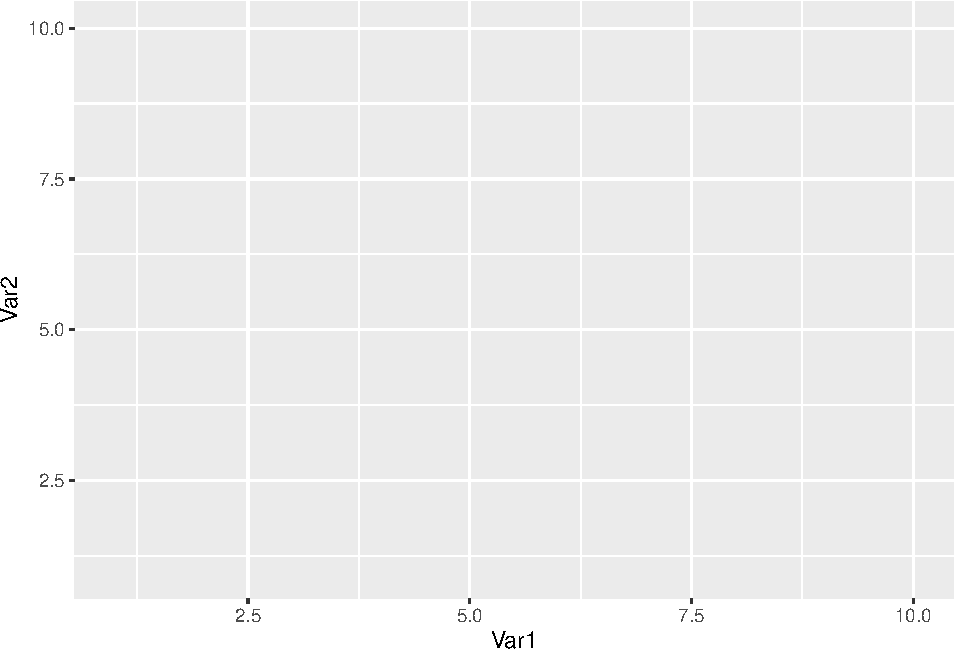
\includegraphics{CFH_R_bookdown_files/figure-latex/unnamed-chunk-152-1.pdf}

Das Ergebnis ist ein leerer Graph, mit der Variable \texttt{Var1} auf der X-Achse und der Variable \texttt{Var2} auf der Y-Achse.

\hypertarget{streu-punktdiagramm}{%
\section{Streu-/Punktdiagramm}\label{streu-punktdiagramm}}

Streudiagramme können Ihnen helfen, die Beziehung zwischen zwei Variablen zu erkennen. Ein Streudiagramm ist eine einfache Darstellung der Kovariation einer Variablen mit einer zweiten Variable.

Besonders gut funktioniert dies, wenn man 2 numerische Variablen gegeneinander plotted.

Im Datensatz \texttt{diamonds} gibt es beispielsweise die Variable \texttt{price} (Kosten des Steins) und die Karatzahl (Masse).

\begin{Shaded}
\begin{Highlighting}[]
\FunctionTok{head}\NormalTok{(diamonds)}
\end{Highlighting}
\end{Shaded}

\begin{verbatim}
## # A tibble: 6 x 10
##   carat cut       color clarity depth table price     x     y     z
##   <dbl> <ord>     <ord> <ord>   <dbl> <dbl> <int> <dbl> <dbl> <dbl>
## 1  0.23 Ideal     E     SI2      61.5    55   326  3.95  3.98  2.43
## 2  0.21 Premium   E     SI1      59.8    61   326  3.89  3.84  2.31
## 3  0.23 Good      E     VS1      56.9    65   327  4.05  4.07  2.31
## 4  0.29 Premium   I     VS2      62.4    58   334  4.2   4.23  2.63
## 5  0.31 Good      J     SI2      63.3    58   335  4.34  4.35  2.75
## 6  0.24 Very Good J     VVS2     62.8    57   336  3.94  3.96  2.48
\end{verbatim}

\hypertarget{streudiagramm-mit-2-variablen}{%
\subsection{Streudiagramm mit 2 Variablen}\label{streudiagramm-mit-2-variablen}}

Stellen wir zunächst einmal unsere Grundfunktion auf:

\begin{Shaded}
\begin{Highlighting}[]
\FunctionTok{ggplot}\NormalTok{(}\AttributeTok{data =}\NormalTok{ diamonds, }\FunctionTok{aes}\NormalTok{(}\AttributeTok{x =}\NormalTok{ carat, }\AttributeTok{y =}\NormalTok{ price))}
\end{Highlighting}
\end{Shaded}

Das Ergebnis ist ein leerer Graph, mit der Variable \texttt{carat} auf der X-Achse und der Variable \texttt{price} auf der Y-Achse. Wir könnten also betrachten, ob der Preis von Diamanten steigt, wenn die Karat (Masse) höher sind.

\hypertarget{geom_point}{%
\subsection{geom\_point()}\label{geom_point}}

Nun fehlen uns nun noch die charakteristischen ``Punkte'', die den Graph zum Streudiagramm machen. Jeder Punkt repräsentiert einen Stein mit einer Karatzahl und einem Preis.

Wir wollen also ein neues Element in unseren Graphen zeichnen,sozusagen eine weitere Schicht auftragen. Dies funktioniert in \texttt{ggplot2} mit dem \texttt{+} Operator. Die Punkte sind eine Geometrie (das 3. Element unserer Grammatik). Geometrie wird i.d.R. mit \texttt{geom} geschrieben:

\begin{Shaded}
\begin{Highlighting}[]
\FunctionTok{ggplot}\NormalTok{(}\AttributeTok{data =}\NormalTok{ diamonds, }\FunctionTok{aes}\NormalTok{(}\AttributeTok{x =}\NormalTok{ carat, }\AttributeTok{y =}\NormalTok{ price)) }\SpecialCharTok{+}
  \FunctionTok{geom\_point}\NormalTok{()}
\end{Highlighting}
\end{Shaded}

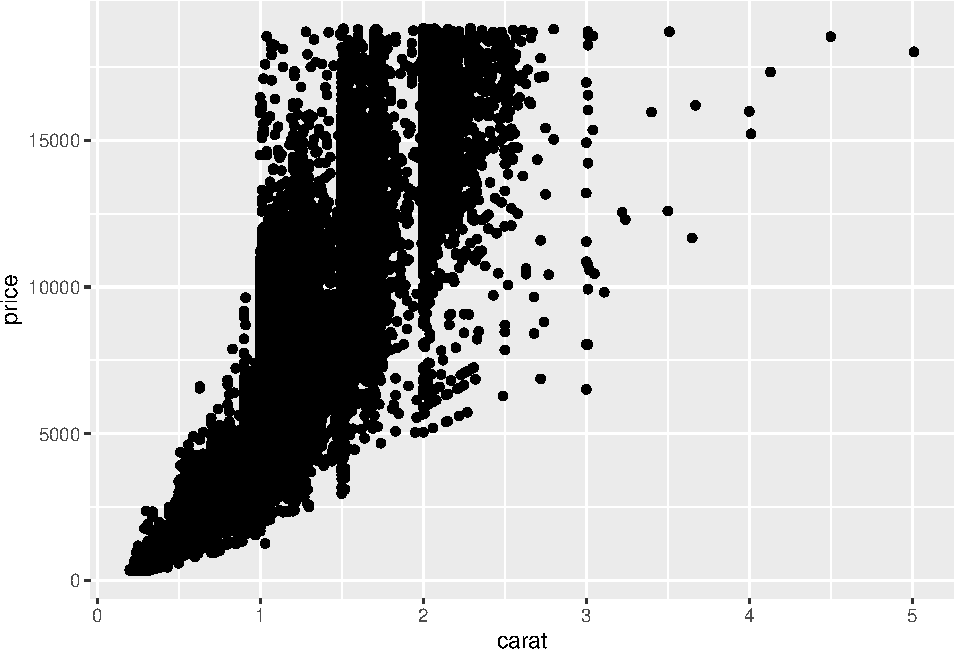
\includegraphics{CFH_R_bookdown_files/figure-latex/unnamed-chunk-155-1.pdf}

Es scheint, als bestünde ein \textbf{positiver} Zusammenhang zwischen \texttt{carat} und \texttt{price}. Mit zunehmender Karatzahl werden Steine also tendenziell teurer.

\hypertarget{geom_smooth}{%
\subsection{geom\_smooth()}\label{geom_smooth}}

Manchmal ist es praktisch in das ``Chaos'' der Punkte des Streudiagramms etwas Ordnung zu bringen und sich die Zusammenhänge noch einmal mit einer linearen Funktion zu visualisieren (Regressionsgerade). Dies lässt sich mit der Funktion \texttt{geom\_smooth()} machen. Wir hängen sie also einfach mit einem weiteren \texttt{+} an unseren Graphen dran:

\begin{Shaded}
\begin{Highlighting}[]
\FunctionTok{ggplot}\NormalTok{(}\AttributeTok{data =}\NormalTok{ diamonds, }\FunctionTok{aes}\NormalTok{(}\AttributeTok{x =}\NormalTok{ carat, }\AttributeTok{y =}\NormalTok{ price)) }\SpecialCharTok{+}
  \FunctionTok{geom\_point}\NormalTok{() }\SpecialCharTok{+}
  \FunctionTok{geom\_smooth}\NormalTok{(}\AttributeTok{method =} \StringTok{"lm"}\NormalTok{)}
\end{Highlighting}
\end{Shaded}

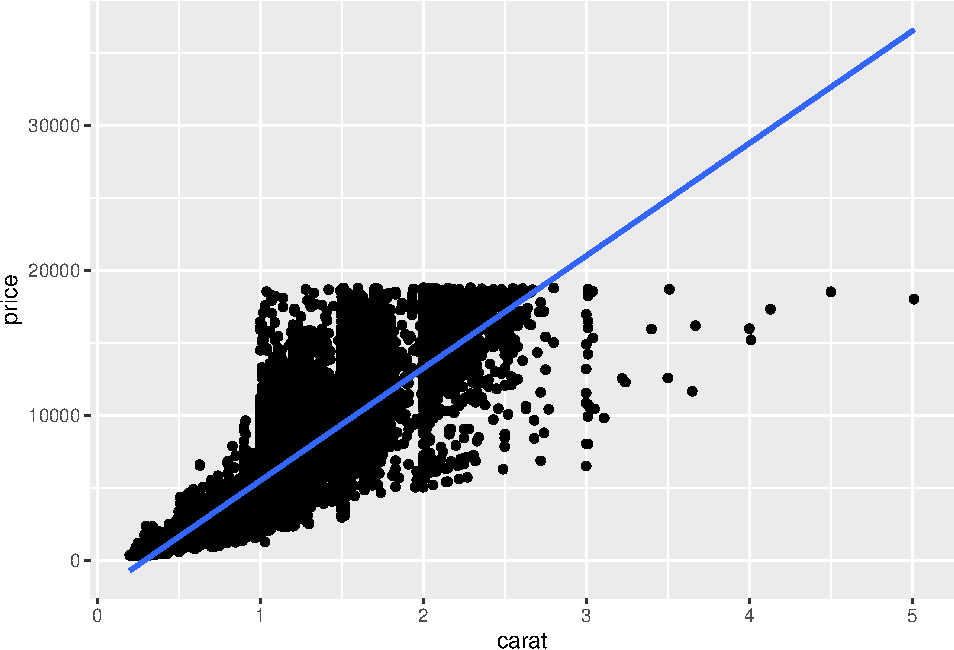
\includegraphics{CFH_R_bookdown_files/figure-latex/unnamed-chunk-156-1.pdf}

Die Angabe \texttt{method\ =\ "lm"} macht die Linie zur Geraden, geben wir dieses Argument nicht an, bekommen wir eine sogenannte loess-Kurve, die jedoch schnell unübersichtlich wird:

\begin{Shaded}
\begin{Highlighting}[]
\FunctionTok{ggplot}\NormalTok{(}\AttributeTok{data =}\NormalTok{ diamonds, }\FunctionTok{aes}\NormalTok{(}\AttributeTok{x =}\NormalTok{ carat, }\AttributeTok{y =}\NormalTok{ price)) }\SpecialCharTok{+}
  \FunctionTok{geom\_point}\NormalTok{() }\SpecialCharTok{+}
  \FunctionTok{geom\_smooth}\NormalTok{()}
\end{Highlighting}
\end{Shaded}

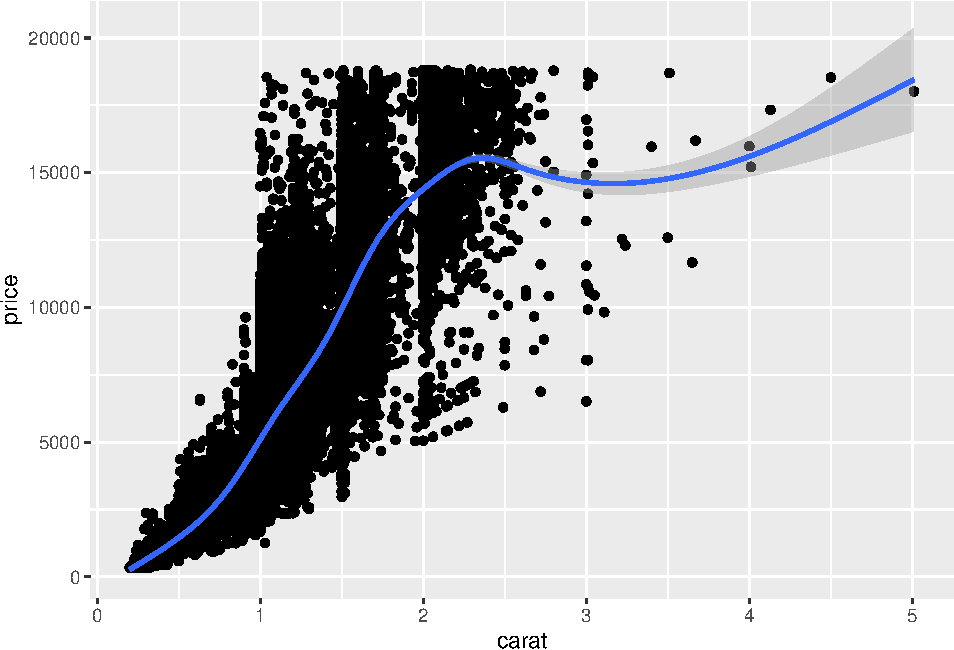
\includegraphics{CFH_R_bookdown_files/figure-latex/unnamed-chunk-157-1.pdf}

\hypertarget{streudiagramm-mit-mehr-als-2-variablen}{%
\subsection{Streudiagramm mit mehr als 2 Variablen}\label{streudiagramm-mit-mehr-als-2-variablen}}

Ein weiteres wichtiges Merkmal eines Diamanten ist sein Schliff, im \texttt{diamonds} Datensatz heißt diese Variable \texttt{cut}. Sie wird in mehreren Kategorien gemessen:

\begin{Shaded}
\begin{Highlighting}[]
\FunctionTok{table}\NormalTok{(diamonds}\SpecialCharTok{$}\NormalTok{cut)}
\end{Highlighting}
\end{Shaded}

\begin{verbatim}
## 
##      Fair      Good Very Good   Premium     Ideal 
##      1610      4906     12082     13791     21551
\end{verbatim}

Wollen wir diese 3. Variable auch in unserem Graphen darstellen, haben wir das Problem, dass wir neben X und Y keine weitere Achse haben. Oft behilft man sich in solchen Situationen durch die Hinzunahme einer weiteren \textbf{aesthetics} Kategorie, z.B. \textbf{Farben} (\texttt{colour}). Jede Schliffkategorie erhält also ihre eigene Farbe:

\begin{Shaded}
\begin{Highlighting}[]
\FunctionTok{ggplot}\NormalTok{(}\AttributeTok{data =}\NormalTok{ diamonds, }\FunctionTok{aes}\NormalTok{(}\AttributeTok{x =}\NormalTok{ carat, }\AttributeTok{y =}\NormalTok{ price, }\AttributeTok{colour =}\NormalTok{ cut)) }\SpecialCharTok{+}
  \FunctionTok{geom\_point}\NormalTok{() }\SpecialCharTok{+}
  \FunctionTok{geom\_smooth}\NormalTok{(}\AttributeTok{method =} \StringTok{"lm"}\NormalTok{)}
\end{Highlighting}
\end{Shaded}

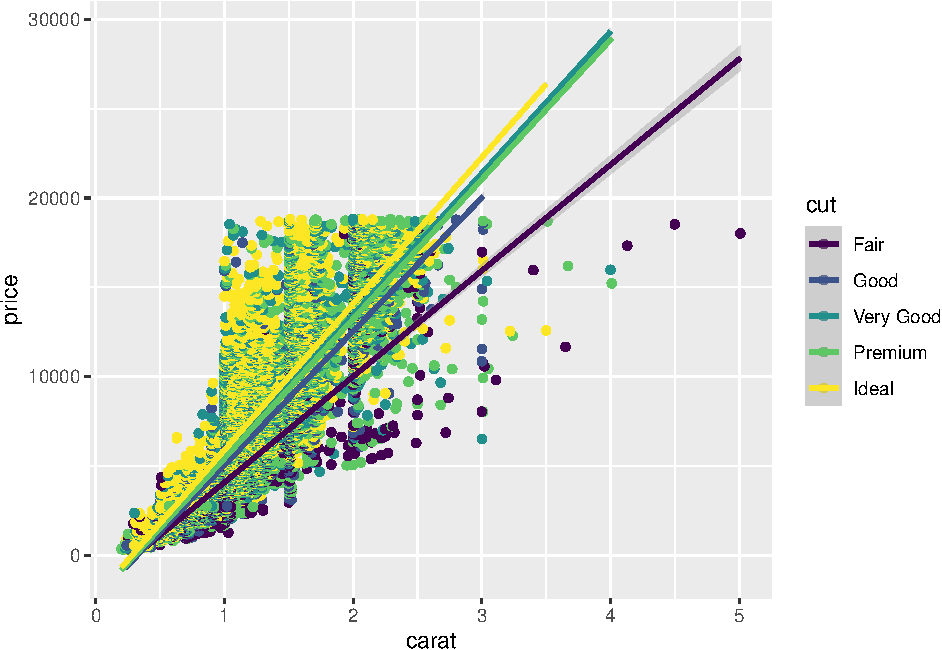
\includegraphics{CFH_R_bookdown_files/figure-latex/unnamed-chunk-159-1.pdf}

Es wären auch andere \textbf{aesthetics} zur Unterscheidung denkbar, z.B. die Form der Punkte (\texttt{shape}):

\begin{Shaded}
\begin{Highlighting}[]
\FunctionTok{ggplot}\NormalTok{(}\AttributeTok{data =}\NormalTok{ diamonds, }\FunctionTok{aes}\NormalTok{(}\AttributeTok{x =}\NormalTok{ carat, }\AttributeTok{y =}\NormalTok{ price, }\AttributeTok{shape =}\NormalTok{ cut)) }\SpecialCharTok{+}
  \FunctionTok{geom\_point}\NormalTok{()}
\end{Highlighting}
\end{Shaded}

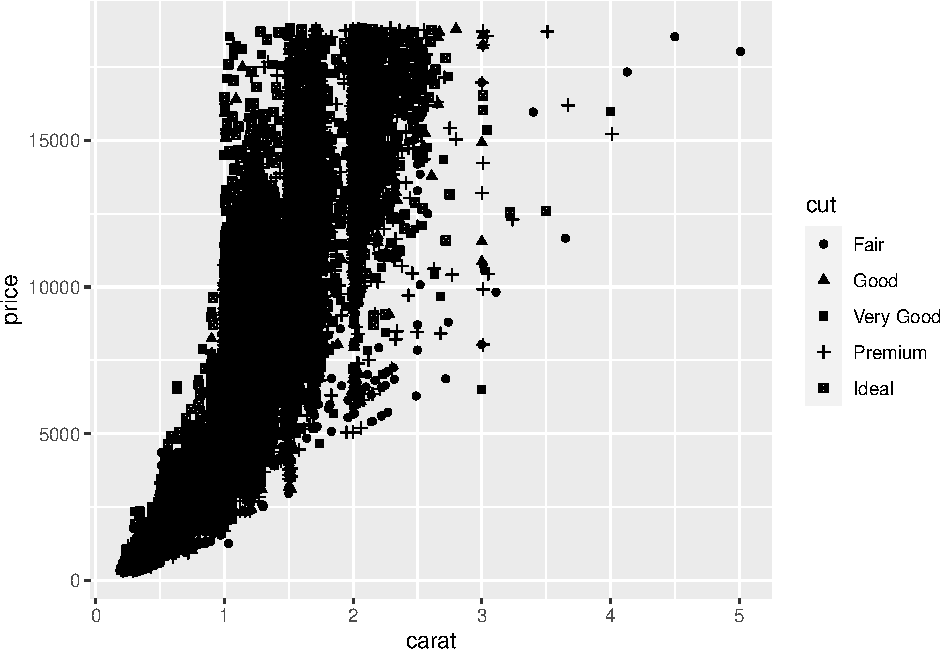
\includegraphics{CFH_R_bookdown_files/figure-latex/unnamed-chunk-160-1.pdf}

\hypertarget{histogramm}{%
\section{Histogramm}\label{histogramm}}

Das Histogramm ist der wichtigste Graph zur Darstellung der Verteilung einer Variable. Er ist hinsichtlich der Komplexität sogar noch etwas leichter als das Streudiagramm, da nur 1 Variable enthalten ist.

Die darzustellende Variable liegt i.d.R. auf der X-Achse, während auf der Y-Achse die absolute oder relative Häufigkeit der Merkmalsausprägungen dargestellt wird.

Lassen Sie uns anhand der Variable \texttt{price} einmal ausprobieren ein Histogramm zu erstellen:

\begin{Shaded}
\begin{Highlighting}[]
\FunctionTok{ggplot}\NormalTok{(}\AttributeTok{data =}\NormalTok{ diamonds, }\FunctionTok{aes}\NormalTok{(}\AttributeTok{x =}\NormalTok{ price)) }\SpecialCharTok{+}
  \FunctionTok{geom\_histogram}\NormalTok{()}
\end{Highlighting}
\end{Shaded}

\begin{verbatim}
## `stat_bin()` using `bins = 30`. Pick better value with `binwidth`.
\end{verbatim}

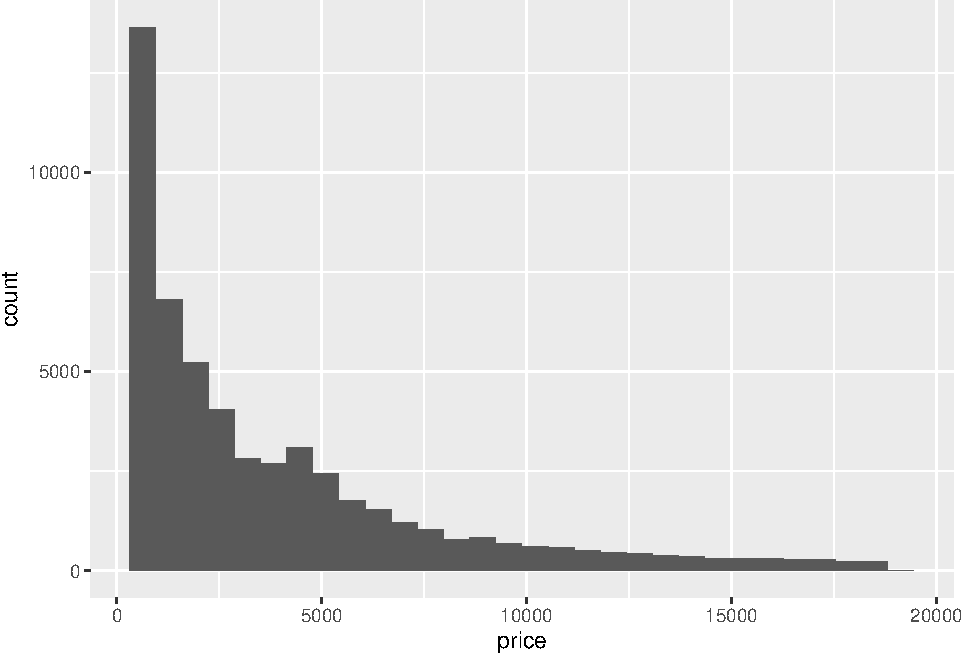
\includegraphics{CFH_R_bookdown_files/figure-latex/unnamed-chunk-161-1.pdf}

Wie wir sehen, kommen günstigere Diamanten häufiger vor als teure. In diesem Fall haben wir also nicht die beliebte \textbf{normalverteilte} Form der Verteilung, sondern eine rechtsschiefte Form.

R gibt uns die Warnmeldung ``Pick better value with \texttt{binwidth}''. Dies ist ein Hinweis, dass die Standardanzahl von 30 Balken für die hohe Auflösung der Variable \texttt{price} nicht ausreicht. Es wird uns eine Auflösung von \texttt{binwidth\ =\ 39} vorgeschlagen:

\begin{Shaded}
\begin{Highlighting}[]
\FunctionTok{ggplot}\NormalTok{(}\AttributeTok{data =}\NormalTok{ diamonds, }\FunctionTok{aes}\NormalTok{(}\AttributeTok{x =}\NormalTok{ price)) }\SpecialCharTok{+}
  \FunctionTok{geom\_histogram}\NormalTok{(}\AttributeTok{binwidth =} \DecValTok{39}\NormalTok{)}
\end{Highlighting}
\end{Shaded}

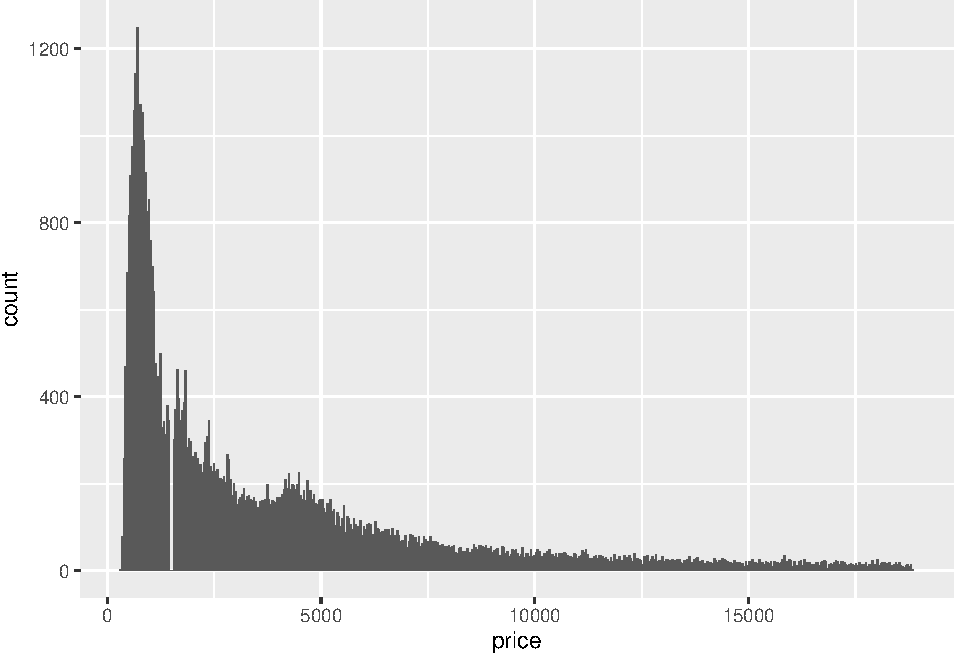
\includegraphics{CFH_R_bookdown_files/figure-latex/unnamed-chunk-162-1.pdf}

\hypertarget{histogramm-fuxfcr-mehrere-gruppen}{%
\subsection{Histogramm für mehrere Gruppen}\label{histogramm-fuxfcr-mehrere-gruppen}}

Natürlich lassen sich Histogramme, also die Verteilungen einer Variable auch getrennt für unterschiedliche Kategorien darstellen:

\begin{Shaded}
\begin{Highlighting}[]
\FunctionTok{ggplot}\NormalTok{(}\AttributeTok{data =}\NormalTok{ diamonds, }\FunctionTok{aes}\NormalTok{(}\AttributeTok{x =}\NormalTok{ price, }\AttributeTok{colour =}\NormalTok{ cut)) }\SpecialCharTok{+}
  \FunctionTok{geom\_histogram}\NormalTok{(}\AttributeTok{binwidth =} \DecValTok{39}\NormalTok{)}
\end{Highlighting}
\end{Shaded}

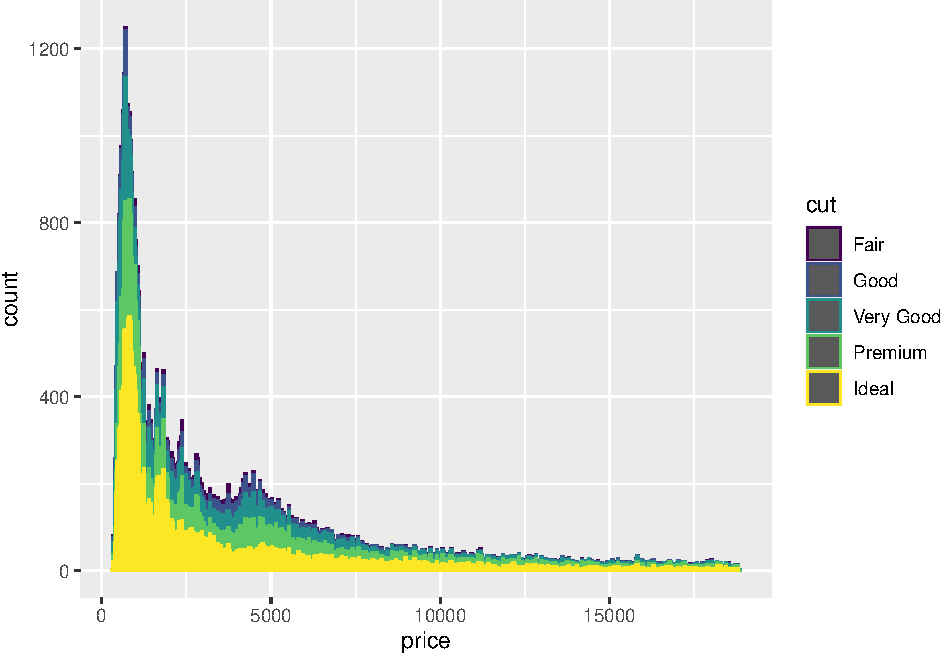
\includegraphics{CFH_R_bookdown_files/figure-latex/unnamed-chunk-163-1.pdf}

\hypertarget{balkendiagramm}{%
\section{Balkendiagramm}\label{balkendiagramm}}

Das Balkendiagramm ist eine Möglichkeit, die Höhe einer Deskriptivstatistik (aka summary statistics) mit der Höhe eines Balkens zu visualisieren. Es wird z.B. eingesetzt, um Gruppenunterschiede, bzw. Unterschiede zwischen den Kategorien einer Variable darzustellen.

Probieren wir es doch gleich einmal mit der Variable \texttt{cut} (Schliff eines Diamanten) aus, die wir oben bereits kennengelernt haben. Wir wollen die durchschnittlichen Karat (Gewicht) der Steine für jede Kategorie von \texttt{cut} darstellen. Die höhe der Balken muss also jeweils den Mittelwert repräsentieren.

Da wir nun keinen Wert visualisieren wollen der ``direkt'' als Zahl im Datensatz steht, sondern für die Berechnung des Mittelwerts eigentlich ein weiterer Rechenschritt erfolgen muss, benutzen wir die \texttt{stat\_summary} Funktion:

\begin{Shaded}
\begin{Highlighting}[]
\FunctionTok{ggplot}\NormalTok{(}\AttributeTok{data =}\NormalTok{ diamonds, }\FunctionTok{aes}\NormalTok{(}\AttributeTok{x =}\NormalTok{ cut, }\AttributeTok{y =}\NormalTok{ carat)) }\SpecialCharTok{+}
  \FunctionTok{stat\_summary}\NormalTok{(}\AttributeTok{geom =} \StringTok{"bar"}\NormalTok{, }\AttributeTok{fun =}\NormalTok{ mean) }
\end{Highlighting}
\end{Shaded}

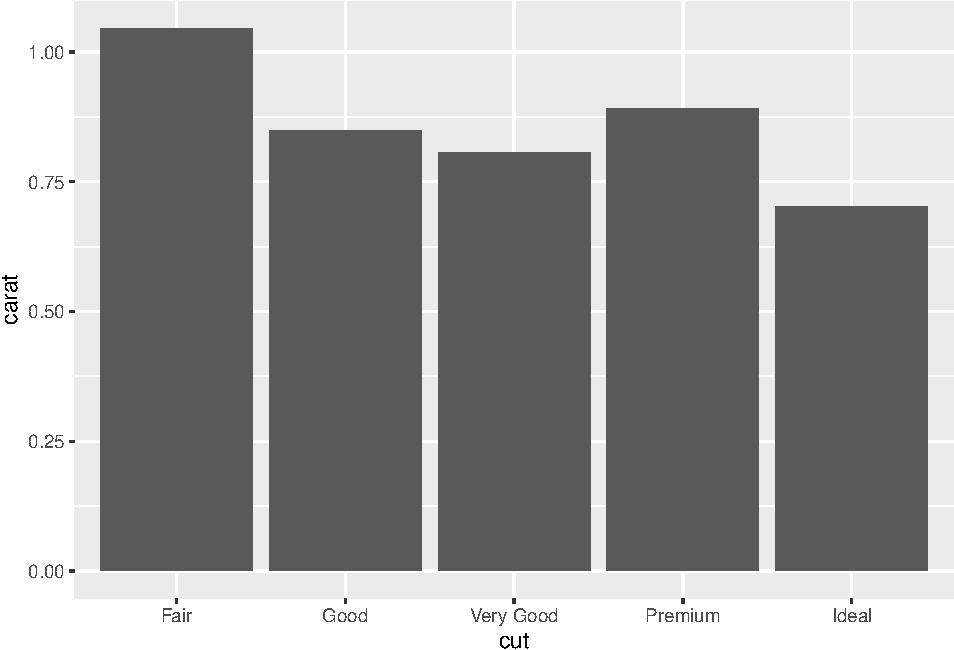
\includegraphics{CFH_R_bookdown_files/figure-latex/unnamed-chunk-164-1.pdf}

Selbiges funktioniert natürlich auch mit jeder anderen Deskriptivstatistik, z.B. dem Median

\begin{Shaded}
\begin{Highlighting}[]
\FunctionTok{ggplot}\NormalTok{(}\AttributeTok{data =}\NormalTok{ diamonds, }\FunctionTok{aes}\NormalTok{(}\AttributeTok{x =}\NormalTok{ cut, }\AttributeTok{y =}\NormalTok{ carat)) }\SpecialCharTok{+}
  \FunctionTok{stat\_summary}\NormalTok{(}\AttributeTok{geom =} \StringTok{"bar"}\NormalTok{, }\AttributeTok{fun =}\NormalTok{ median) }
\end{Highlighting}
\end{Shaded}

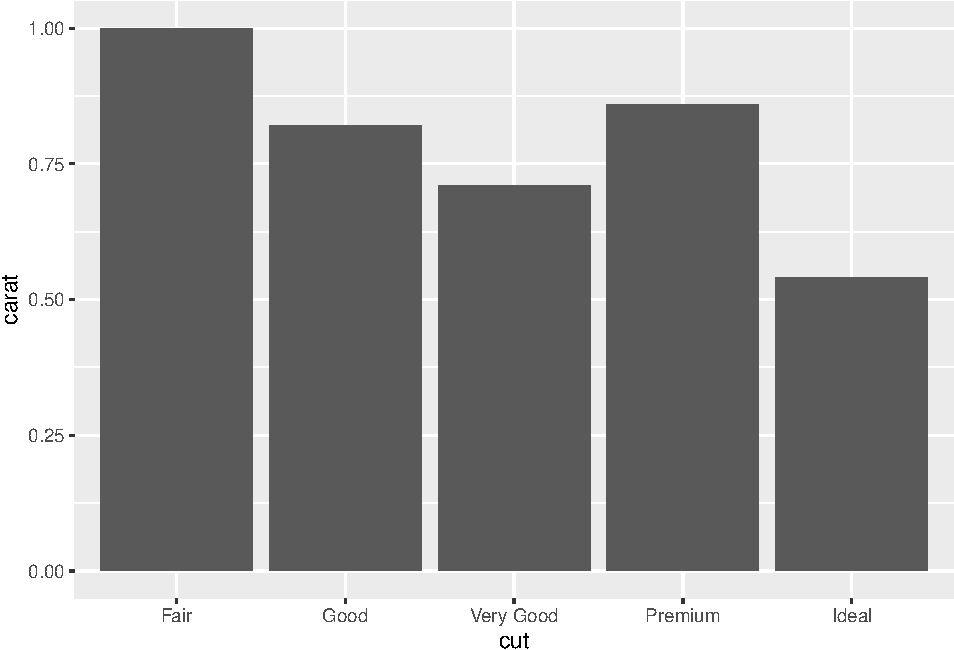
\includegraphics{CFH_R_bookdown_files/figure-latex/unnamed-chunk-165-1.pdf}

Oder theoretisch auch mit anderen \texttt{geoms}

\begin{Shaded}
\begin{Highlighting}[]
\FunctionTok{ggplot}\NormalTok{(}\AttributeTok{data =}\NormalTok{ diamonds, }\FunctionTok{aes}\NormalTok{(}\AttributeTok{x =}\NormalTok{ cut, }\AttributeTok{y =}\NormalTok{ carat)) }\SpecialCharTok{+}
  \FunctionTok{stat\_summary}\NormalTok{(}\AttributeTok{geom =} \StringTok{"point"}\NormalTok{, }\AttributeTok{fun =}\NormalTok{ mean) }
\end{Highlighting}
\end{Shaded}

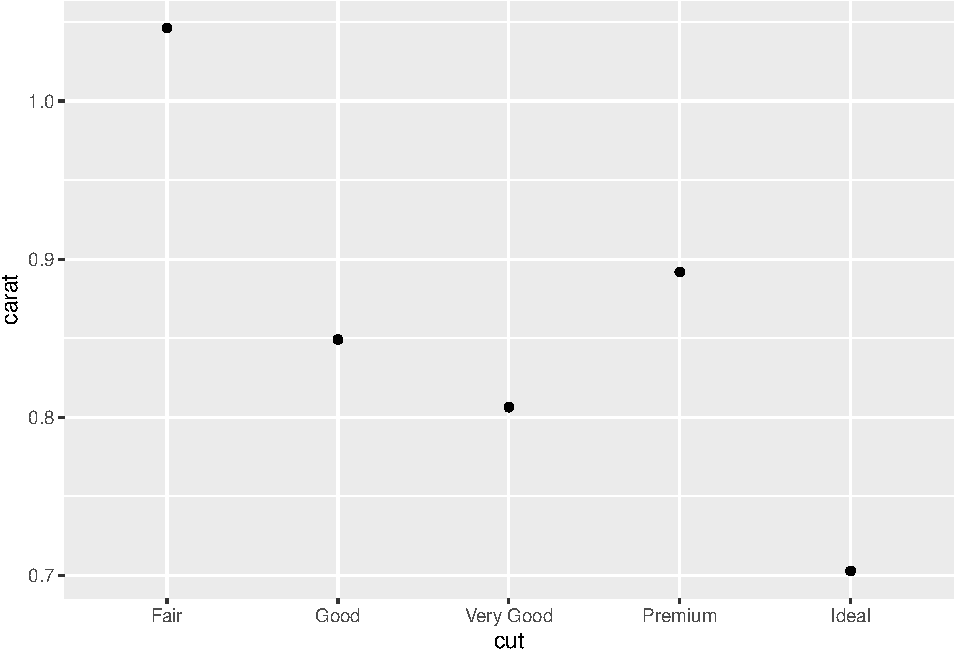
\includegraphics{CFH_R_bookdown_files/figure-latex/unnamed-chunk-166-1.pdf}

Häufig möchte man zusätzlich eine Art von Streuung/Unschärfe darstellen, wenn Mittelwerte dargestellt werden. Eine beliebte Variante ist es, das 95\% Konfidenzintervall um den Mittelwert mit sogenannten \textbf{Fehlerbalken} (error bars) zu visualisieren. Vorher installieren und laden wir noch das Paket \texttt{Hmisc}, welches uns die Berechnung der Fehlerbalken ermöglicht:

\begin{Shaded}
\begin{Highlighting}[]
\FunctionTok{library}\NormalTok{(Hmisc)}
\end{Highlighting}
\end{Shaded}

\begin{verbatim}
## Warning: package 'Hmisc' was built under R version 3.6.2
\end{verbatim}

\begin{verbatim}
## Loading required package: lattice
\end{verbatim}

\begin{verbatim}
## Warning: package 'lattice' was built under R version 3.6.2
\end{verbatim}

\begin{verbatim}
## Loading required package: survival
\end{verbatim}

\begin{verbatim}
## Warning: package 'survival' was built under R version 3.6.2
\end{verbatim}

\begin{verbatim}
## Loading required package: Formula
\end{verbatim}

\begin{verbatim}
## Warning: package 'Formula' was built under R version 3.6.2
\end{verbatim}

\begin{verbatim}
## 
## Attaching package: 'Hmisc'
\end{verbatim}

\begin{verbatim}
## The following object is masked from 'package:psych':
## 
##     describe
\end{verbatim}

\begin{verbatim}
## The following objects are masked from 'package:dplyr':
## 
##     src, summarize
\end{verbatim}

\begin{verbatim}
## The following objects are masked from 'package:base':
## 
##     format.pval, units
\end{verbatim}

\begin{Shaded}
\begin{Highlighting}[]
\FunctionTok{ggplot}\NormalTok{(}\AttributeTok{data =}\NormalTok{ diamonds, }\FunctionTok{aes}\NormalTok{(}\AttributeTok{x =}\NormalTok{ cut, }\AttributeTok{y =}\NormalTok{ carat)) }\SpecialCharTok{+}
  \FunctionTok{stat\_summary}\NormalTok{(}\AttributeTok{fun.data =}\NormalTok{ mean\_cl\_normal,  }\AttributeTok{geom =} \StringTok{"errorbar"}\NormalTok{) }\SpecialCharTok{+}
  \FunctionTok{stat\_summary}\NormalTok{(}\AttributeTok{geom =} \StringTok{"point"}\NormalTok{, }\AttributeTok{fun =}\NormalTok{ mean) }
\end{Highlighting}
\end{Shaded}

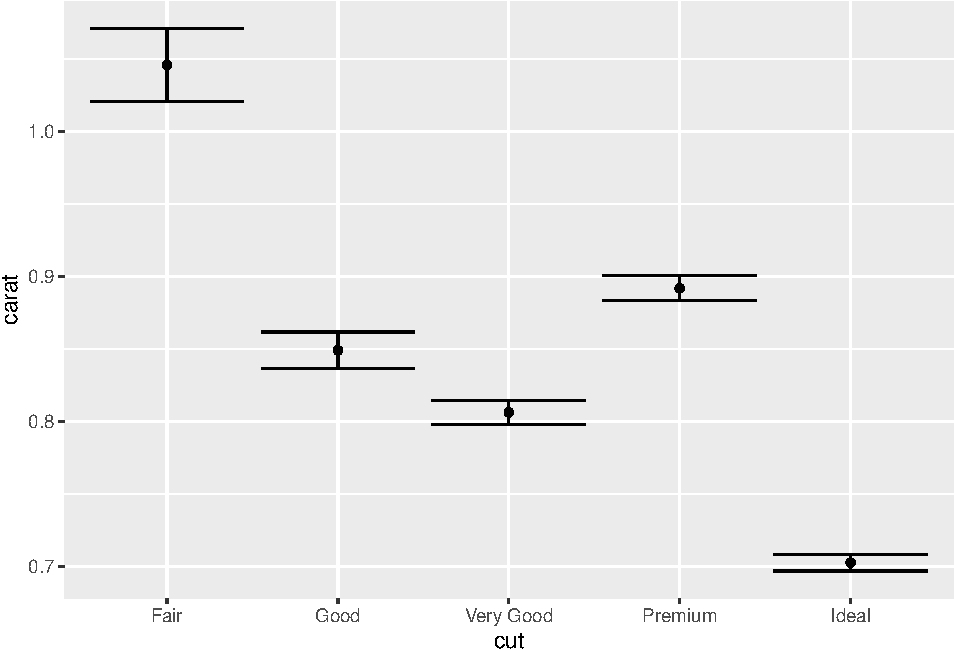
\includegraphics{CFH_R_bookdown_files/figure-latex/unnamed-chunk-167-1.pdf}

\hypertarget{balkendiagramm-mit-mehr-als-3-variablen}{%
\section{Balkendiagramm mit mehr als 3 Variablen}\label{balkendiagramm-mit-mehr-als-3-variablen}}

Genau wie beim Streudiagramm lässt sich das Balkendiagramm auch für mehr als 2 Variablen darstellen. Statt Farben oder Punktfarben ist die einfachste Art Balken zu differenzieren mit der \texttt{fill} Ästhetik:

\begin{Shaded}
\begin{Highlighting}[]
\FunctionTok{ggplot}\NormalTok{(}\AttributeTok{data =}\NormalTok{ diamonds, }\FunctionTok{aes}\NormalTok{(}\AttributeTok{x =}\NormalTok{ cut, }\AttributeTok{y =}\NormalTok{ carat, }\AttributeTok{fill =}\NormalTok{ clarity)) }\SpecialCharTok{+}
  \FunctionTok{stat\_summary}\NormalTok{(}\AttributeTok{geom =} \StringTok{"bar"}\NormalTok{, }\AttributeTok{fun =}\NormalTok{ mean, }\AttributeTok{position =} \FunctionTok{position\_dodge2}\NormalTok{(.}\DecValTok{95}\NormalTok{))}
\end{Highlighting}
\end{Shaded}

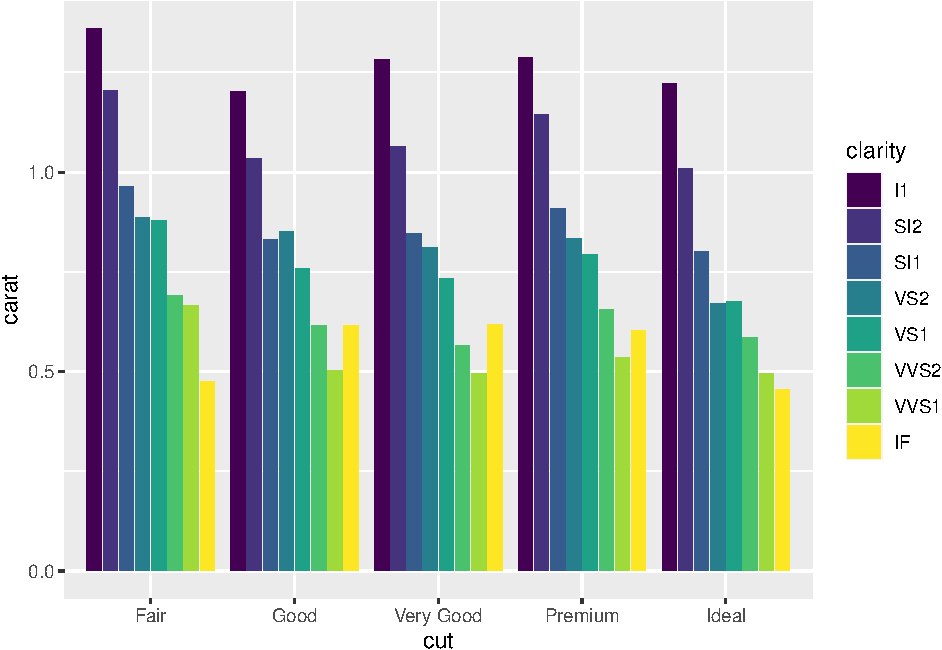
\includegraphics{CFH_R_bookdown_files/figure-latex/unnamed-chunk-168-1.pdf}

Das Argument \texttt{position\_dodge2()} sorgt dafür, dass die Balken nebeneinander positioniert sind und nicht voreinander. Probieren Sie den Code gerne auch einmal ohne \texttt{position\_dodge2()} aus.

\hypertarget{boxplot}{%
\section{Boxplot}\label{boxplot}}

Ähnlich wie das Balkendiagramm, lassen sich Gruppenunterschiede gut mit einem Boxplot darstellen. Dieses zeigt standardmäßig den Median (Mittelbalken), sowie die Streuung der Daten mittels der Box (Quartilabstand, IQR) und die sogenannten Whiskers (1.5 * Quartilabstand). Punkte außerhalb der Whiskers werden als Ausreißer mit einem Punkt gekennzeichnet.

\begin{Shaded}
\begin{Highlighting}[]
\FunctionTok{ggplot}\NormalTok{(}\AttributeTok{data =}\NormalTok{ diamonds, }\FunctionTok{aes}\NormalTok{(}\AttributeTok{x =}\NormalTok{ cut, }\AttributeTok{y =}\NormalTok{ carat)) }\SpecialCharTok{+}
  \FunctionTok{geom\_boxplot}\NormalTok{()}
\end{Highlighting}
\end{Shaded}

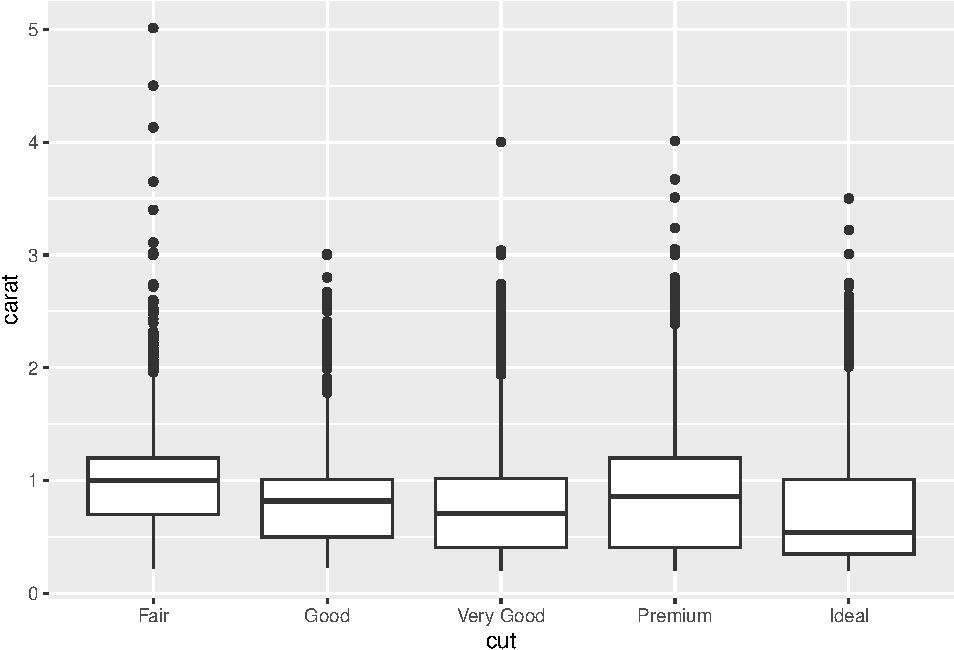
\includegraphics{CFH_R_bookdown_files/figure-latex/unnamed-chunk-169-1.pdf}

\hypertarget{facetting}{%
\section{Facetting}\label{facetting}}

Wir sehen uns noch einmal unser 3-farbiges Streudiagramm von zuvor an:

\begin{Shaded}
\begin{Highlighting}[]
\FunctionTok{ggplot}\NormalTok{(}\AttributeTok{data =}\NormalTok{ diamonds, }\FunctionTok{aes}\NormalTok{(}\AttributeTok{x =}\NormalTok{ carat, }\AttributeTok{y =}\NormalTok{ price, }\AttributeTok{colour =}\NormalTok{ cut)) }\SpecialCharTok{+}
  \FunctionTok{geom\_point}\NormalTok{() }\SpecialCharTok{+}
  \FunctionTok{geom\_smooth}\NormalTok{(}\AttributeTok{method =} \StringTok{"lm"}\NormalTok{)}
\end{Highlighting}
\end{Shaded}

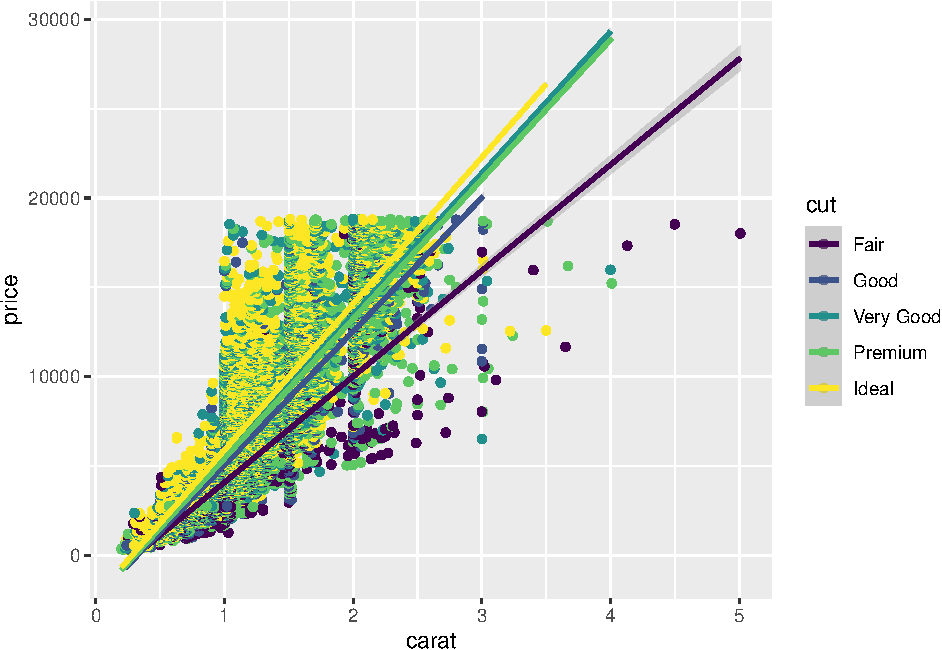
\includegraphics{CFH_R_bookdown_files/figure-latex/unnamed-chunk-170-1.pdf}

Es ist sichtbar, dass die Darstellung vieler Kategorien mittels weiterer aesthetics, wie Farben, Füllungen, Punktarten, etc. schnell unübersichtlich wird.

Oft ist es nützlich, durch die Darstellung einzelner Gruppen in Teilgraphen (Facetten) etwas mehr Klarheit in die Darstellung zu bringen. Der Befehl dafür ist \texttt{facet\_grid()}:

\begin{Shaded}
\begin{Highlighting}[]
\FunctionTok{ggplot}\NormalTok{(}\AttributeTok{data =}\NormalTok{ diamonds, }\FunctionTok{aes}\NormalTok{(}\AttributeTok{x =}\NormalTok{ carat, }\AttributeTok{y =}\NormalTok{ price, }\AttributeTok{colour =}\NormalTok{ cut)) }\SpecialCharTok{+}
  \FunctionTok{geom\_point}\NormalTok{() }\SpecialCharTok{+}
  \FunctionTok{geom\_smooth}\NormalTok{(}\AttributeTok{method =} \StringTok{"lm"}\NormalTok{) }\SpecialCharTok{+}
  \FunctionTok{facet\_grid}\NormalTok{(}\AttributeTok{cols =} \FunctionTok{vars}\NormalTok{(cut))}
\end{Highlighting}
\end{Shaded}

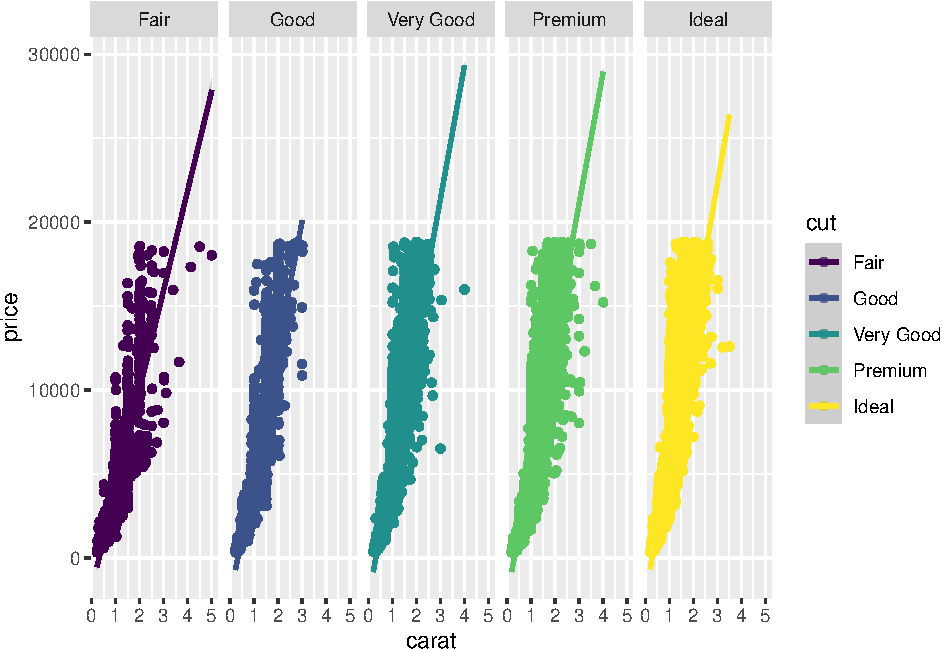
\includegraphics{CFH_R_bookdown_files/figure-latex/unnamed-chunk-171-1.pdf}

Es ist auch eine reihenweise Darstellung möglich

\begin{Shaded}
\begin{Highlighting}[]
\FunctionTok{ggplot}\NormalTok{(}\AttributeTok{data =}\NormalTok{ diamonds, }\FunctionTok{aes}\NormalTok{(}\AttributeTok{x =}\NormalTok{ carat, }\AttributeTok{y =}\NormalTok{ price, }\AttributeTok{colour =}\NormalTok{ cut)) }\SpecialCharTok{+}
  \FunctionTok{geom\_point}\NormalTok{() }\SpecialCharTok{+}
  \FunctionTok{geom\_smooth}\NormalTok{(}\AttributeTok{method =} \StringTok{"lm"}\NormalTok{) }\SpecialCharTok{+}
  \FunctionTok{facet\_grid}\NormalTok{(}\AttributeTok{rows =} \FunctionTok{vars}\NormalTok{(cut))}
\end{Highlighting}
\end{Shaded}

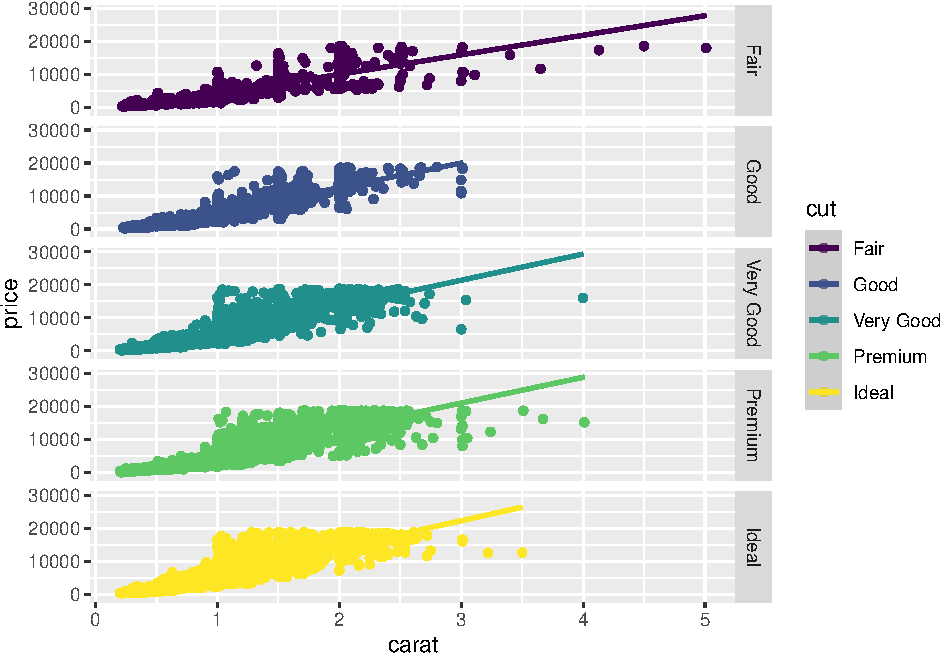
\includegraphics{CFH_R_bookdown_files/figure-latex/unnamed-chunk-172-1.pdf}

\hypertarget{uxe4sthetische-anpassungen}{%
\section{Ästhetische Anpassungen}\label{uxe4sthetische-anpassungen}}

Zum Gewinnen eines schnellen Überblicks kommen wir mit den vorgestellten Darstellungsoptionen schon recht weit. Für eine Publikation oder das Verwenden der Graphik in einer Abschlussarbeit wollen wir jedoch ggf. noch einige Dinge anpassen

\hypertarget{ggtitle}{%
\subsection{ggtitle()}\label{ggtitle}}

Um unserer Graphik einen Titel zu geben, nutzen wir den Befehl \texttt{ggtitle()}. Vorsicht: Wie jede Zeichenkette schreiben wir auch hier den Namen in Anführungszeichen:

\begin{Shaded}
\begin{Highlighting}[]
\FunctionTok{ggplot}\NormalTok{(}\AttributeTok{data =}\NormalTok{ diamonds, }\FunctionTok{aes}\NormalTok{(}\AttributeTok{x =}\NormalTok{ carat, }\AttributeTok{y =}\NormalTok{ price, }\AttributeTok{colour =}\NormalTok{ cut)) }\SpecialCharTok{+}
  \FunctionTok{geom\_point}\NormalTok{() }\SpecialCharTok{+}
  \FunctionTok{geom\_smooth}\NormalTok{(}\AttributeTok{method =} \StringTok{"lm"}\NormalTok{) }\SpecialCharTok{+}
  \FunctionTok{ggtitle}\NormalTok{(}\StringTok{"Abb 1: Streudiagramm Diamantenpreis"}\NormalTok{)}
\end{Highlighting}
\end{Shaded}

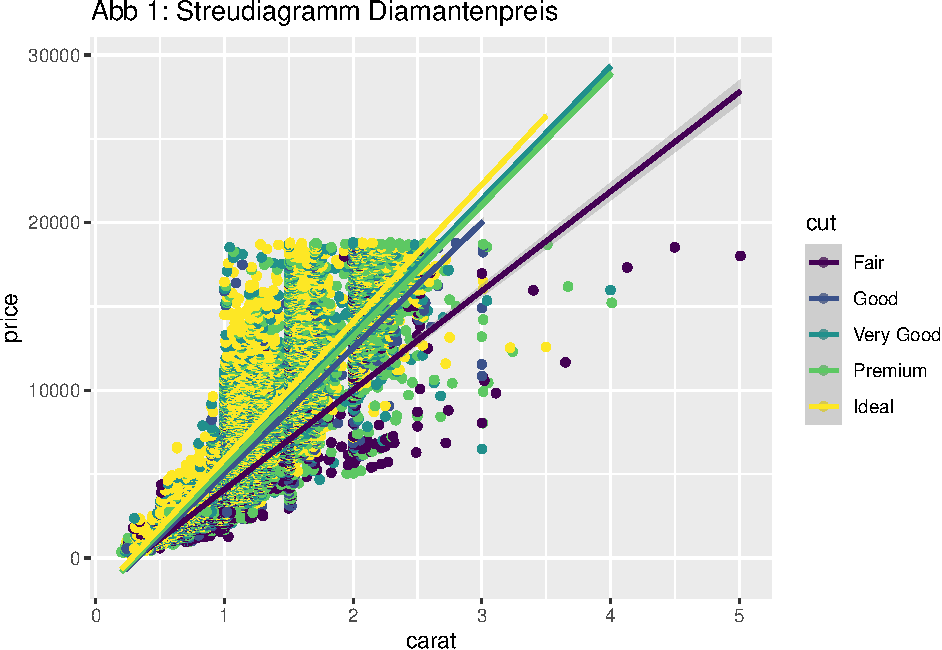
\includegraphics{CFH_R_bookdown_files/figure-latex/unnamed-chunk-173-1.pdf}

\hypertarget{labs}{%
\subsection{labs()}\label{labs}}

\texttt{ggplot2} benutzt zur Beschriftung von X- und Y-Achse sowie als Titel der Legende automatisch die im \texttt{data.frame} enthaltenen Variablennamen

\begin{Shaded}
\begin{Highlighting}[]
\FunctionTok{names}\NormalTok{(diamonds)}
\end{Highlighting}
\end{Shaded}

\begin{verbatim}
##  [1] "carat"   "cut"     "color"   "clarity" "depth"   "table"   "price"  
##  [8] "x"       "y"       "z"
\end{verbatim}

Wollen wir dort eine schönere Beschriftung verwenden, nutzen den Befehl \texttt{labs()}. Die Y-Achse wollen wir nun auf deutsch ``Preis'' nennen, die X-Achse ``Karat'' und die Legende soll den Titel ``Schliff'' haben:

\begin{Shaded}
\begin{Highlighting}[]
\FunctionTok{ggplot}\NormalTok{(}\AttributeTok{data =}\NormalTok{ diamonds, }\FunctionTok{aes}\NormalTok{(}\AttributeTok{x =}\NormalTok{ carat, }\AttributeTok{y =}\NormalTok{ price, }\AttributeTok{colour =}\NormalTok{ cut)) }\SpecialCharTok{+}
  \FunctionTok{geom\_point}\NormalTok{() }\SpecialCharTok{+}
  \FunctionTok{geom\_smooth}\NormalTok{(}\AttributeTok{method =} \StringTok{"lm"}\NormalTok{) }\SpecialCharTok{+}
  \FunctionTok{labs}\NormalTok{(}\AttributeTok{x =} \StringTok{"Karat"}\NormalTok{, }\AttributeTok{y =} \StringTok{"Preis"}\NormalTok{, }\AttributeTok{colour =} \StringTok{"Schliff"}\NormalTok{)}
\end{Highlighting}
\end{Shaded}

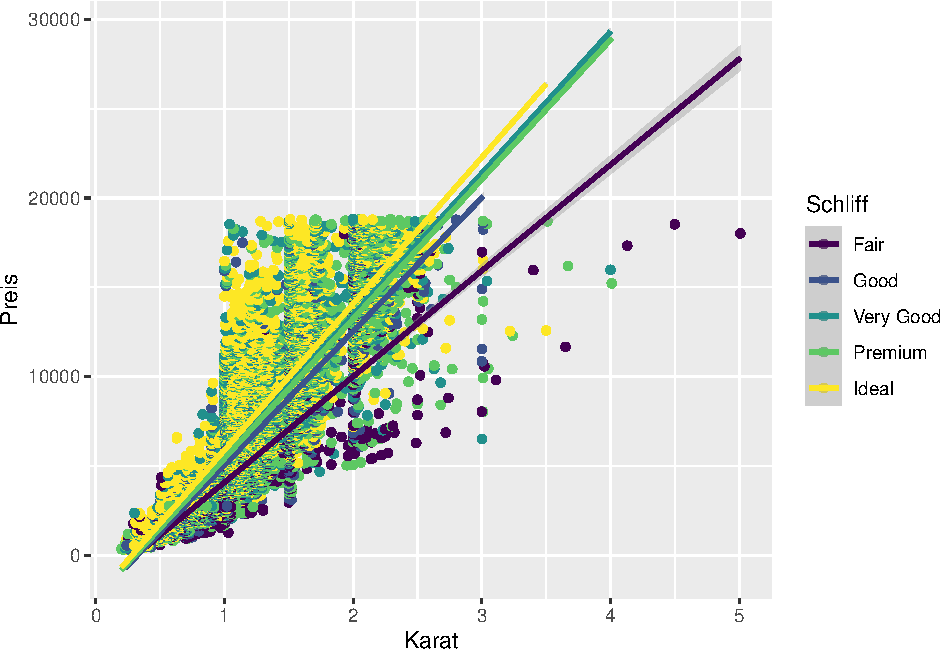
\includegraphics{CFH_R_bookdown_files/figure-latex/unnamed-chunk-175-1.pdf}

\hypertarget{achsen-veruxe4ndern}{%
\subsection{Achsen verändern}\label{achsen-veruxe4ndern}}

Auch die Einheiten, mit denen die Achsen beschriftet werden (axis ticks) werden von R automatisch und gleichmäßig gewählt. Die Beschriftung kann auch manuell gesteuert werden. Der Befehl lautet \texttt{scale\_x\_continuous()}, bzw. \texttt{scale\_y\_continuous()} für kontinuierliche (numerische) X- und Y-Achsen. Für kategoriale X- und Y-Achsen (Namen/Kategorien) lautet der Befehl \texttt{scale\_x\_discrete()}, bzw. \texttt{scale\_y\_discrete\ ()}.

Wir wollen zum Üben in dem vorangegangenen Graphen auf der X-Achse (Karat) manuell nur die Werte 0, 2 und 4 zulassen. Dies erfolgt über \texttt{breaks\ =\ c()}:

\begin{Shaded}
\begin{Highlighting}[]
\FunctionTok{ggplot}\NormalTok{(}\AttributeTok{data =}\NormalTok{ diamonds, }\FunctionTok{aes}\NormalTok{(}\AttributeTok{x =}\NormalTok{ carat, }\AttributeTok{y =}\NormalTok{ price, }\AttributeTok{colour =}\NormalTok{ cut)) }\SpecialCharTok{+}
  \FunctionTok{geom\_point}\NormalTok{() }\SpecialCharTok{+}
  \FunctionTok{geom\_smooth}\NormalTok{(}\AttributeTok{method =} \StringTok{"lm"}\NormalTok{) }\SpecialCharTok{+}
  \FunctionTok{labs}\NormalTok{(}\AttributeTok{x =} \StringTok{"Karat"}\NormalTok{, }\AttributeTok{y =} \StringTok{"Preis"}\NormalTok{, }\AttributeTok{colour =} \StringTok{"Schliff"}\NormalTok{) }\SpecialCharTok{+}
  \FunctionTok{scale\_x\_continuous}\NormalTok{(}\AttributeTok{breaks =} \FunctionTok{c}\NormalTok{(}\DecValTok{0}\NormalTok{, }\DecValTok{2}\NormalTok{, }\DecValTok{4}\NormalTok{))}
\end{Highlighting}
\end{Shaded}

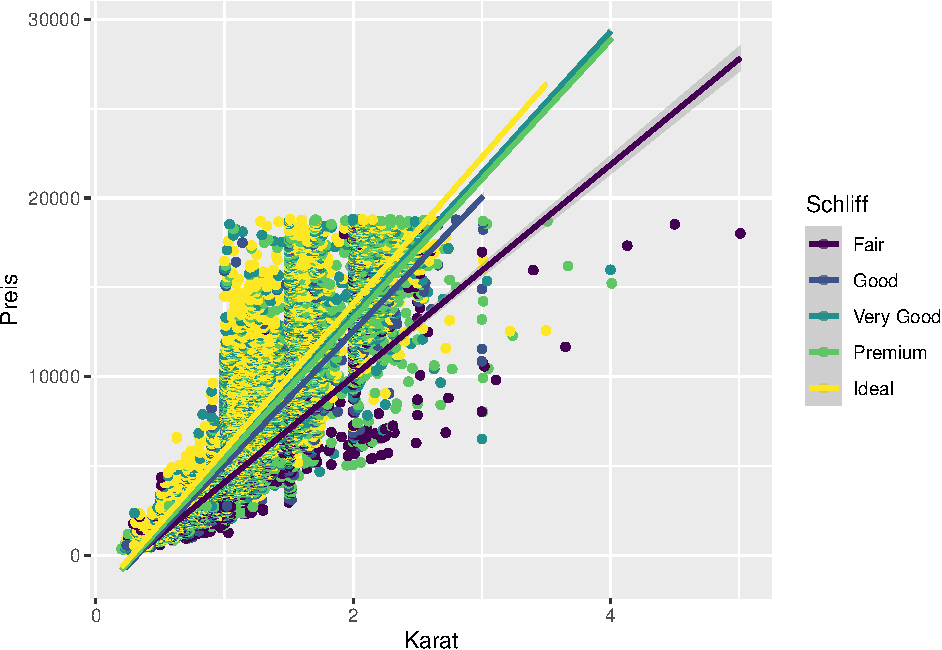
\includegraphics{CFH_R_bookdown_files/figure-latex/unnamed-chunk-176-1.pdf}

Automatisch werden an den angegebenen Positionen der kontinuierlichen X-Achse die Zahlen eingetragen, also 0, 2 und 4. Wir könnten diese aber auch mit \texttt{labels} versehen:

\begin{Shaded}
\begin{Highlighting}[]
\FunctionTok{ggplot}\NormalTok{(}\AttributeTok{data =}\NormalTok{ diamonds, }\FunctionTok{aes}\NormalTok{(}\AttributeTok{x =}\NormalTok{ carat, }\AttributeTok{y =}\NormalTok{ price, }\AttributeTok{colour =}\NormalTok{ cut)) }\SpecialCharTok{+}
  \FunctionTok{geom\_point}\NormalTok{() }\SpecialCharTok{+}
  \FunctionTok{geom\_smooth}\NormalTok{(}\AttributeTok{method =} \StringTok{"lm"}\NormalTok{) }\SpecialCharTok{+}
  \FunctionTok{labs}\NormalTok{(}\AttributeTok{x =} \StringTok{"Karat"}\NormalTok{, }\AttributeTok{y =} \StringTok{"Preis"}\NormalTok{, }\AttributeTok{colour =} \StringTok{"Schliff"}\NormalTok{) }\SpecialCharTok{+}
  \FunctionTok{scale\_x\_continuous}\NormalTok{(}\AttributeTok{breaks =} \FunctionTok{c}\NormalTok{(}\DecValTok{0}\NormalTok{, }\DecValTok{2}\NormalTok{, }\DecValTok{4}\NormalTok{), }\AttributeTok{labels =} \FunctionTok{c}\NormalTok{(}\StringTok{"Null"}\NormalTok{, }\StringTok{"Zwei"}\NormalTok{, }\StringTok{"Vier"}\NormalTok{))}
\end{Highlighting}
\end{Shaded}

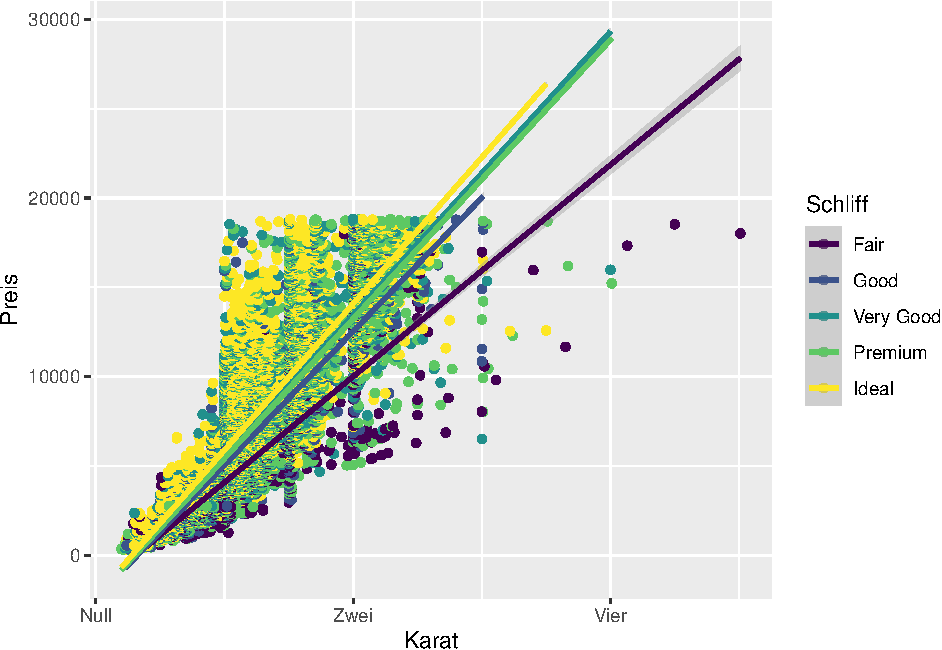
\includegraphics{CFH_R_bookdown_files/figure-latex/unnamed-chunk-177-1.pdf}

\hypertarget{theme}{%
\section{theme()}\label{theme}}

Der Befehl \texttt{theme()} ist einer der mächtigsten in \texttt{ggplot2}, denn er verändert das Aussehen des gesamten Graphen.

Er hat so viele Anpassungsmöglichkeiten, dass wir sie an dieser Stelle unmöglich auflisten könnten. Glücklicherweise ist eine Liste aller Optionen unter \texttt{?theme()} hinterlegt.

\hypertarget{elemente-von-theme}{%
\subsection{Elemente von theme()}\label{elemente-von-theme}}

Sehen wir uns dennoch einmal ein Beispiel an. Wie wäre es, wenn wir den gesamten Text in unserem Graphen etwas kleiner machen? Das geht so:

\begin{Shaded}
\begin{Highlighting}[]
\FunctionTok{ggplot}\NormalTok{(}\AttributeTok{data =}\NormalTok{ diamonds, }\FunctionTok{aes}\NormalTok{(}\AttributeTok{x =}\NormalTok{ carat, }\AttributeTok{y =}\NormalTok{ price, }\AttributeTok{colour =}\NormalTok{ cut)) }\SpecialCharTok{+}
  \FunctionTok{geom\_point}\NormalTok{() }\SpecialCharTok{+}
  \FunctionTok{geom\_smooth}\NormalTok{(}\AttributeTok{method =} \StringTok{"lm"}\NormalTok{) }\SpecialCharTok{+}
  \FunctionTok{labs}\NormalTok{(}\AttributeTok{x =} \StringTok{"Karat"}\NormalTok{, }\AttributeTok{y =} \StringTok{"Preis"}\NormalTok{, }\AttributeTok{colour =} \StringTok{"Schliff"}\NormalTok{) }\SpecialCharTok{+}
  \FunctionTok{theme}\NormalTok{(}\AttributeTok{text =} \FunctionTok{element\_text}\NormalTok{(}\AttributeTok{size =} \DecValTok{5}\NormalTok{))}
\end{Highlighting}
\end{Shaded}

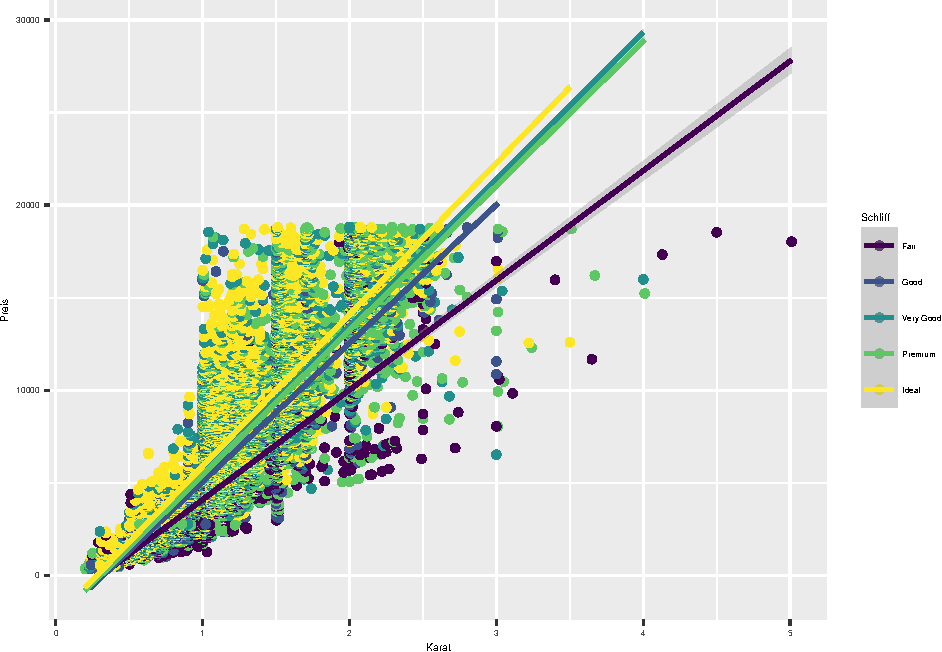
\includegraphics{CFH_R_bookdown_files/figure-latex/unnamed-chunk-178-1.pdf}

Wir können auf diese Art auch Elemente (Achsen, Beschriftungen\ldots) aus unserem Graphen löschen. Dafür wählt man die Option \texttt{element\_blank()}. Lassen wir zum Beispiel einmal die kleinen Striche, die die Einheiten an den Achsen anzeigen verschwinden:

\begin{Shaded}
\begin{Highlighting}[]
\FunctionTok{ggplot}\NormalTok{(}\AttributeTok{data =}\NormalTok{ diamonds, }\FunctionTok{aes}\NormalTok{(}\AttributeTok{x =}\NormalTok{ carat, }\AttributeTok{y =}\NormalTok{ price, }\AttributeTok{colour =}\NormalTok{ cut)) }\SpecialCharTok{+}
  \FunctionTok{geom\_point}\NormalTok{() }\SpecialCharTok{+}
  \FunctionTok{geom\_smooth}\NormalTok{(}\AttributeTok{method =} \StringTok{"lm"}\NormalTok{) }\SpecialCharTok{+}
  \FunctionTok{labs}\NormalTok{(}\AttributeTok{x =} \StringTok{"Karat"}\NormalTok{, }\AttributeTok{y =} \StringTok{"Preis"}\NormalTok{, }\AttributeTok{colour =} \StringTok{"Schliff"}\NormalTok{) }\SpecialCharTok{+}
  \FunctionTok{theme}\NormalTok{(}\AttributeTok{axis.ticks =} \FunctionTok{element\_blank}\NormalTok{())}
\end{Highlighting}
\end{Shaded}

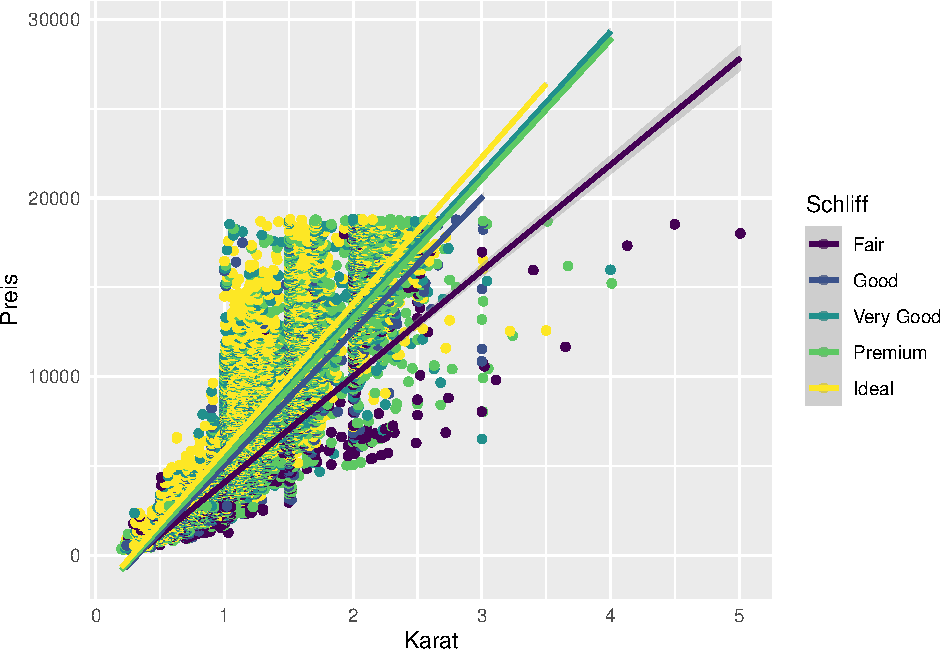
\includegraphics{CFH_R_bookdown_files/figure-latex/unnamed-chunk-179-1.pdf}

\hypertarget{legende}{%
\subsection{Legende}\label{legende}}

Auch die Legende des Graphen lässt sich über \texttt{theme()} steuern. Dazu nutzen wir das Argument \texttt{legend.position}.

Die Optionen sind ``right'' (das ist der Standard), ``left'', ``top'', ``bottom''. Lassen Sie uns die Legende einmal unter den Graphen verschieben:

\begin{Shaded}
\begin{Highlighting}[]
\FunctionTok{ggplot}\NormalTok{(}\AttributeTok{data =}\NormalTok{ diamonds, }\FunctionTok{aes}\NormalTok{(}\AttributeTok{x =}\NormalTok{ carat, }\AttributeTok{y =}\NormalTok{ price, }\AttributeTok{colour =}\NormalTok{ cut)) }\SpecialCharTok{+}
  \FunctionTok{geom\_point}\NormalTok{() }\SpecialCharTok{+}
  \FunctionTok{geom\_smooth}\NormalTok{(}\AttributeTok{method =} \StringTok{"lm"}\NormalTok{) }\SpecialCharTok{+}
  \FunctionTok{labs}\NormalTok{(}\AttributeTok{x =} \StringTok{"Karat"}\NormalTok{, }\AttributeTok{y =} \StringTok{"Preis"}\NormalTok{, }\AttributeTok{colour =} \StringTok{"Schliff"}\NormalTok{) }\SpecialCharTok{+}
  \FunctionTok{theme}\NormalTok{(}\AttributeTok{legend.position =} \StringTok{"bottom"}\NormalTok{)}
\end{Highlighting}
\end{Shaded}

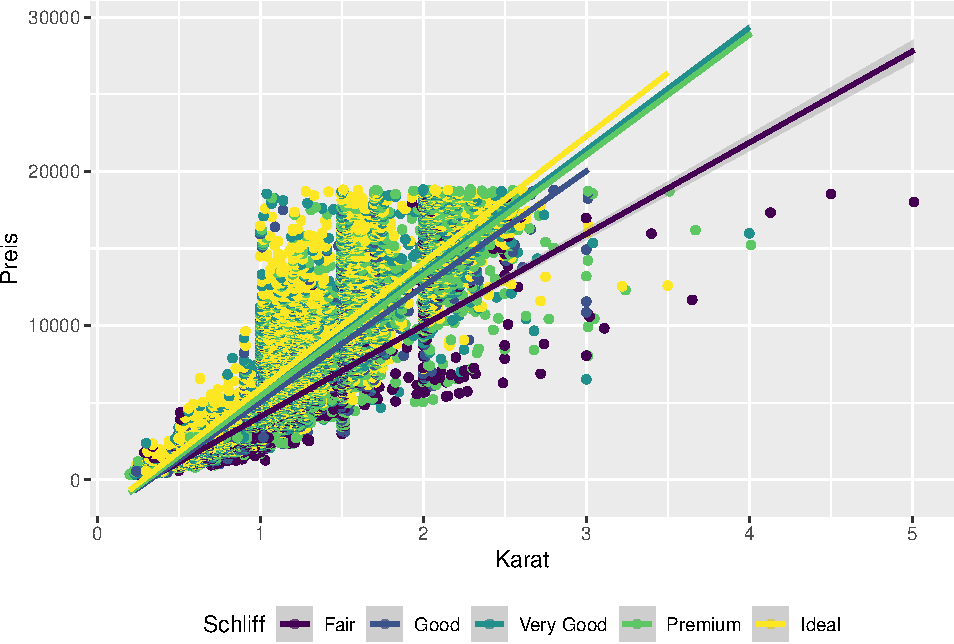
\includegraphics{CFH_R_bookdown_files/figure-latex/unnamed-chunk-180-1.pdf}

\hypertarget{vorgefertigte-themes}{%
\subsection{Vorgefertigte themes}\label{vorgefertigte-themes}}

Wenn wir nicht alle optischen Elemente des Graphen einzeln anpassen möchten, aber ihn doch etwas individueller aussehen lassen wollen, können wir eines der vorgefertigten Themen nutzen.

Hier einige häufig gewählte Beispiele:

\begin{Shaded}
\begin{Highlighting}[]
\FunctionTok{ggplot}\NormalTok{(}\AttributeTok{data =}\NormalTok{ diamonds, }\FunctionTok{aes}\NormalTok{(}\AttributeTok{x =}\NormalTok{ carat, }\AttributeTok{y =}\NormalTok{ price, }\AttributeTok{colour =}\NormalTok{ cut)) }\SpecialCharTok{+}
  \FunctionTok{geom\_point}\NormalTok{() }\SpecialCharTok{+}
  \FunctionTok{geom\_smooth}\NormalTok{(}\AttributeTok{method =} \StringTok{"lm"}\NormalTok{) }\SpecialCharTok{+}
  \FunctionTok{labs}\NormalTok{(}\AttributeTok{x =} \StringTok{"Karat"}\NormalTok{, }\AttributeTok{y =} \StringTok{"Preis"}\NormalTok{, }\AttributeTok{colour =} \StringTok{"Schliff"}\NormalTok{) }\SpecialCharTok{+}
  \FunctionTok{theme\_bw}\NormalTok{()}
\end{Highlighting}
\end{Shaded}

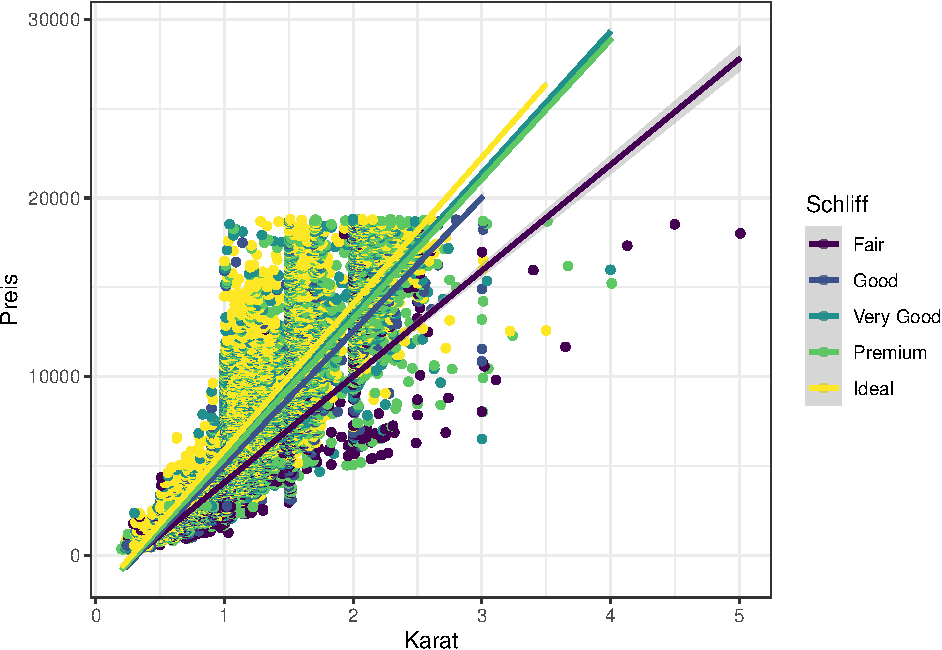
\includegraphics{CFH_R_bookdown_files/figure-latex/unnamed-chunk-181-1.pdf}

\begin{Shaded}
\begin{Highlighting}[]
\FunctionTok{ggplot}\NormalTok{(}\AttributeTok{data =}\NormalTok{ diamonds, }\FunctionTok{aes}\NormalTok{(}\AttributeTok{x =}\NormalTok{ carat, }\AttributeTok{y =}\NormalTok{ price, }\AttributeTok{colour =}\NormalTok{ cut)) }\SpecialCharTok{+}
  \FunctionTok{geom\_point}\NormalTok{() }\SpecialCharTok{+}
  \FunctionTok{geom\_smooth}\NormalTok{(}\AttributeTok{method =} \StringTok{"lm"}\NormalTok{) }\SpecialCharTok{+}
  \FunctionTok{labs}\NormalTok{(}\AttributeTok{x =} \StringTok{"Karat"}\NormalTok{, }\AttributeTok{y =} \StringTok{"Preis"}\NormalTok{, }\AttributeTok{colour =} \StringTok{"Schliff"}\NormalTok{) }\SpecialCharTok{+}
  \FunctionTok{theme\_classic}\NormalTok{()}
\end{Highlighting}
\end{Shaded}

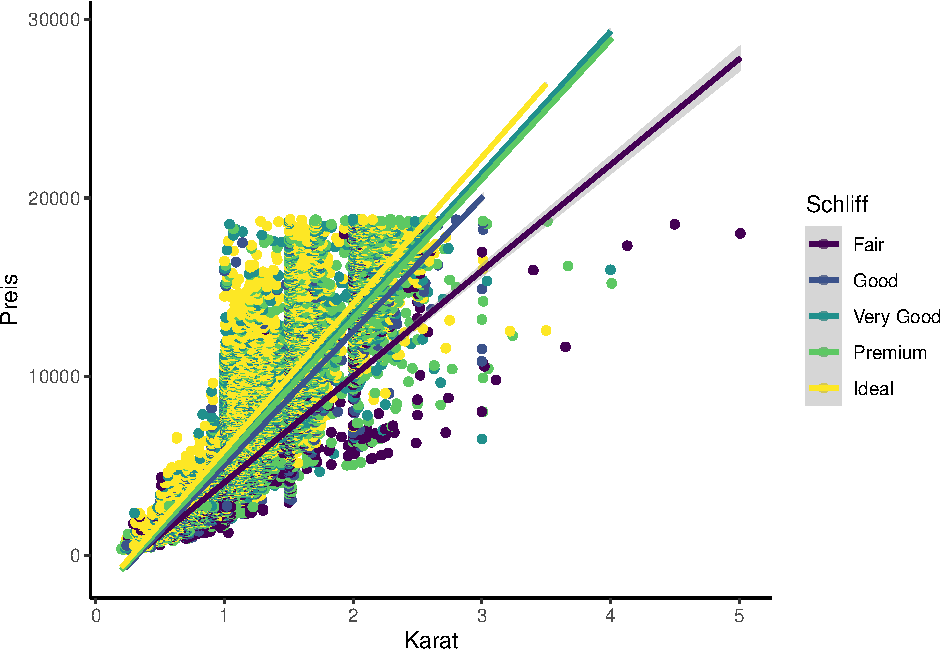
\includegraphics{CFH_R_bookdown_files/figure-latex/unnamed-chunk-182-1.pdf}

\begin{Shaded}
\begin{Highlighting}[]
\FunctionTok{ggplot}\NormalTok{(}\AttributeTok{data =}\NormalTok{ diamonds, }\FunctionTok{aes}\NormalTok{(}\AttributeTok{x =}\NormalTok{ carat, }\AttributeTok{y =}\NormalTok{ price, }\AttributeTok{colour =}\NormalTok{ cut)) }\SpecialCharTok{+}
  \FunctionTok{geom\_point}\NormalTok{() }\SpecialCharTok{+}
  \FunctionTok{geom\_smooth}\NormalTok{(}\AttributeTok{method =} \StringTok{"lm"}\NormalTok{) }\SpecialCharTok{+}
  \FunctionTok{labs}\NormalTok{(}\AttributeTok{x =} \StringTok{"Karat"}\NormalTok{, }\AttributeTok{y =} \StringTok{"Preis"}\NormalTok{, }\AttributeTok{colour =} \StringTok{"Schliff"}\NormalTok{) }\SpecialCharTok{+}
  \FunctionTok{theme\_dark}\NormalTok{()}
\end{Highlighting}
\end{Shaded}

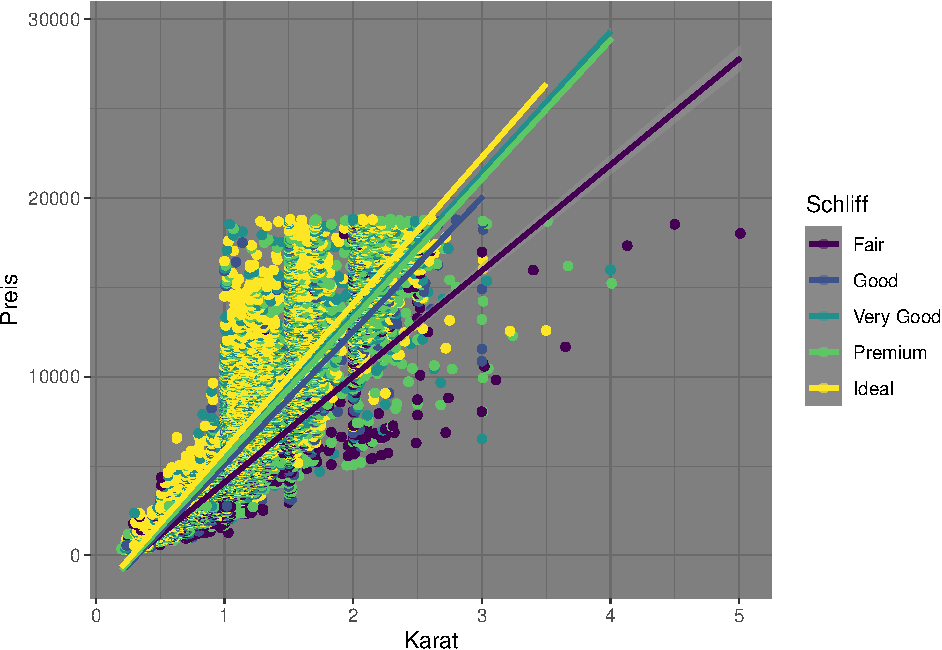
\includegraphics{CFH_R_bookdown_files/figure-latex/unnamed-chunk-183-1.pdf}

Es gibt R-Pakete, die hunderte weitere Optionen bereitstellen, so zum Beispiel das Paket \texttt{ggthemes}. Installieren Sie es einfach mittels \texttt{install.packages()} und testen Sie es aus.

\hypertarget{abbildungen-kombinieren}{%
\section{Abbildungen kombinieren}\label{abbildungen-kombinieren}}

Gerade bei komplexeren Fragestellungen oder Studien mit mehreren abhängigen Variablen (AVs) kommt es vor, dass die Anzahl der Graphen etwas zu groß wird.

Dann kann es helfen, mehrere Graphen zu einem kombinierte Graph zusammenzusetzen. Die Funktion dafür heißt \texttt{ggarrange()} und kommt aus dem R-Paket \texttt{ggpubr}.

Also installieren Sie kurz das Paket \texttt{ggpubr}, laden es mittels \texttt{library()} und dann geht es gleich weiter:

\begin{Shaded}
\begin{Highlighting}[]
\CommentTok{\# install.packages("ggpubr")}
\FunctionTok{library}\NormalTok{(ggpubr)}
\end{Highlighting}
\end{Shaded}

Damit es sich auch lohnt, nehmen wir uns gleich einmal 4 Graphen vor. Nehmen wir doch einen von jeder Art. Damit es nicht zu unübersichtlich wird, benennen wir die 4 Graphen mit \texttt{a}, \texttt{b}, \texttt{c} und \texttt{d}:

\begin{Shaded}
\begin{Highlighting}[]
\NormalTok{a }\OtherTok{=} \FunctionTok{ggplot}\NormalTok{(}\AttributeTok{data =}\NormalTok{ diamonds, }\FunctionTok{aes}\NormalTok{(}\AttributeTok{x =}\NormalTok{ price)) }\SpecialCharTok{+}
  \FunctionTok{geom\_histogram}\NormalTok{()}

\NormalTok{b }\OtherTok{=} \FunctionTok{ggplot}\NormalTok{(}\AttributeTok{data =}\NormalTok{ diamonds, }\FunctionTok{aes}\NormalTok{(}\AttributeTok{x =}\NormalTok{ carat, }\AttributeTok{y =}\NormalTok{ price)) }\SpecialCharTok{+}
  \FunctionTok{geom\_point}\NormalTok{()}

\NormalTok{c }\OtherTok{=} \FunctionTok{ggplot}\NormalTok{(}\AttributeTok{data =}\NormalTok{ diamonds, }\FunctionTok{aes}\NormalTok{(}\AttributeTok{x =}\NormalTok{ color, }\AttributeTok{y =}\NormalTok{ carat)) }\SpecialCharTok{+}
  \FunctionTok{stat\_summary}\NormalTok{(}\AttributeTok{geom =} \StringTok{"bar"}\NormalTok{, }\AttributeTok{fun =}\NormalTok{ mean) }

\NormalTok{d }\OtherTok{=} \FunctionTok{ggplot}\NormalTok{(}\AttributeTok{data =}\NormalTok{ diamonds, }\FunctionTok{aes}\NormalTok{(}\AttributeTok{x =}\NormalTok{ price)) }\SpecialCharTok{+}
  \FunctionTok{geom\_boxplot}\NormalTok{()}
\end{Highlighting}
\end{Shaded}

Diese 4 Objekte \texttt{a}, \texttt{b}, \texttt{c} und \texttt{d} setzen wir dann einfach in \texttt{ggarrange()} ein. Es macht Sinn den Graphen auch ein Label zu geben, dann kann man in der Fußnote der Abbildung darauf verweise, was in welchem Graphen zu sehen ist (z.B. ``\emph{In Graphik A sieht man ein Histogramm von\ldots{}}''):

\begin{Shaded}
\begin{Highlighting}[]
\FunctionTok{ggarrange}\NormalTok{(a, b, c, d, }\AttributeTok{labels =} \FunctionTok{c}\NormalTok{(}\StringTok{"A"}\NormalTok{, }\StringTok{"B"}\NormalTok{, }\StringTok{"C"}\NormalTok{, }\StringTok{"D"}\NormalTok{))}
\end{Highlighting}
\end{Shaded}

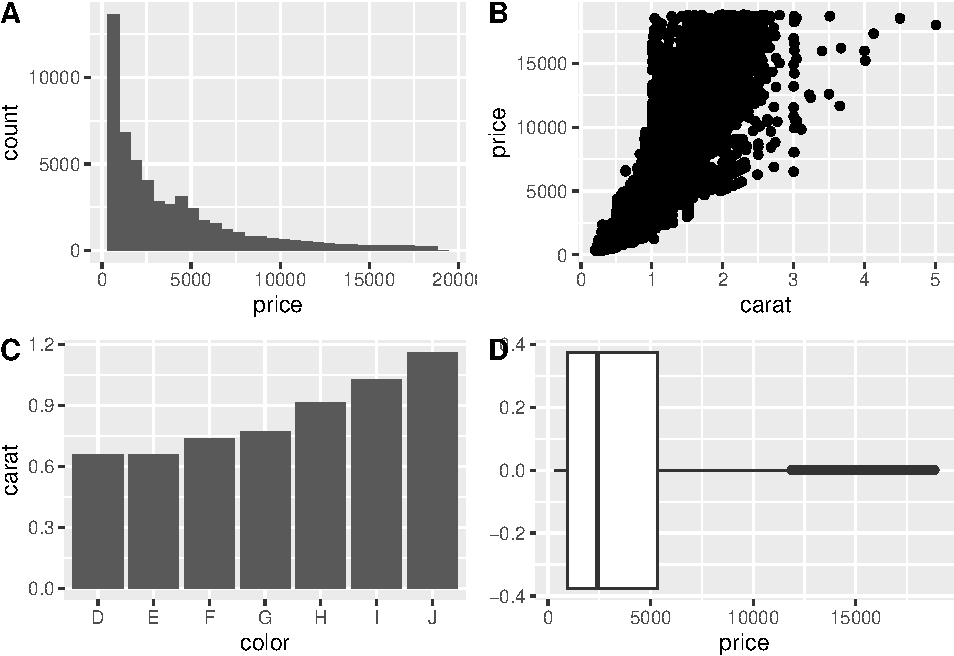
\includegraphics{CFH_R_bookdown_files/figure-latex/unnamed-chunk-186-1.pdf}

Wir können auch steuern, wie das Gitter der Graphen zusammengesetzt sein soll, zum Beispiel untereinander\ldots{}

\begin{Shaded}
\begin{Highlighting}[]
\FunctionTok{ggarrange}\NormalTok{(a, b, }\AttributeTok{nrow =} \DecValTok{2}\NormalTok{)}
\end{Highlighting}
\end{Shaded}

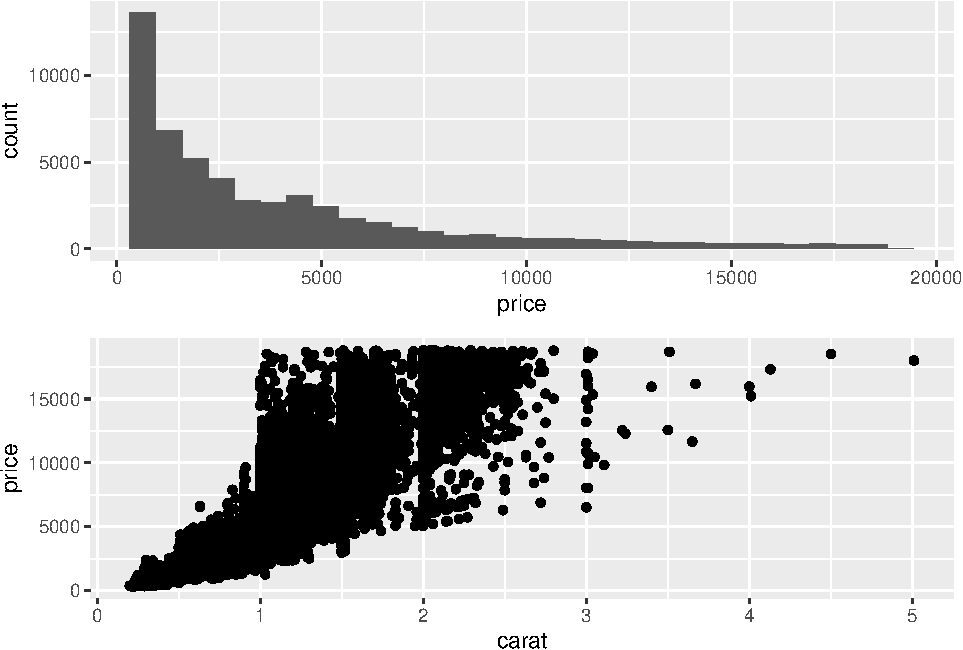
\includegraphics{CFH_R_bookdown_files/figure-latex/unnamed-chunk-187-1.pdf}

\ldots{} oder nebeneinander:

\begin{Shaded}
\begin{Highlighting}[]
\FunctionTok{ggarrange}\NormalTok{(a, b, }\AttributeTok{ncol =} \DecValTok{2}\NormalTok{)}
\end{Highlighting}
\end{Shaded}

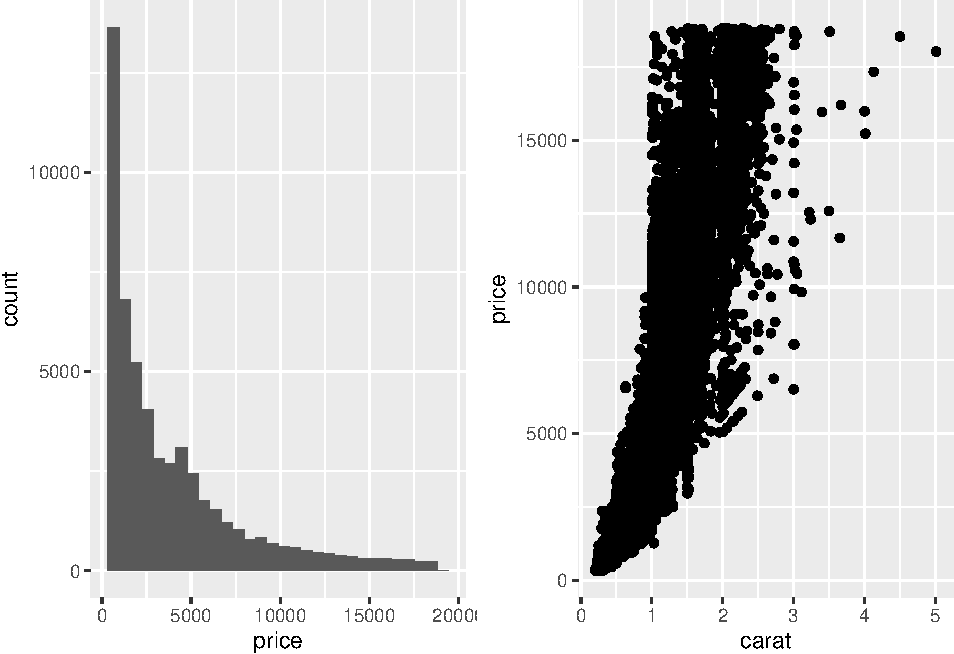
\includegraphics{CFH_R_bookdown_files/figure-latex/unnamed-chunk-188-1.pdf}

\hypertarget{abbildungen-exportieren}{%
\section{Abbildungen exportieren}\label{abbildungen-exportieren}}

Der Export der Graphen meint im Prinzip folgendes: Speichere mir den Graphen in mein Arbeitsverzeichnis und das in einem gängigen Bildformat (.pdf, .png, .jpg, .tif\ldots).

Das Vorgehen funktioniert für alle Formate gleich:

\begin{enumerate}
\def\labelenumi{\arabic{enumi}.}
\item
  Wenn noch nicht geschehen, mit \texttt{setwd()} das gewünschte Arbeitsverzeichnnis setzen
\item
  Mittels Befehl angeben, welche Art von Export gewünscht ist, z.B. \texttt{png()}
\item
  Den Code für den \texttt{ggplot()} Graphen ausführen
\item
  Mit dem Befehl \texttt{dev.off()} anzeigen, dass der Code für den Graphen fertig ist, die Datei also geschrieben werden soll.
\end{enumerate}

Größe (in cm) und Auflösung (in dpi) lassen sich direkt innerhalb des Befehls steuern.

Ein Beispiel:

\begin{Shaded}
\begin{Highlighting}[]
\FunctionTok{png}\NormalTok{(}\AttributeTok{file =} \StringTok{"Figure1.png"}\NormalTok{, }\AttributeTok{width =} \DecValTok{5}\NormalTok{, }\AttributeTok{height =} \DecValTok{5}\NormalTok{, }\AttributeTok{units =} \StringTok{"in"}\NormalTok{, }\AttributeTok{res =} \DecValTok{300}\NormalTok{)}

\FunctionTok{ggplot}\NormalTok{(}\AttributeTok{data =}\NormalTok{ diamonds, }\FunctionTok{aes}\NormalTok{(}\AttributeTok{x =}\NormalTok{ price, }\AttributeTok{colour =}\NormalTok{ cut)) }\SpecialCharTok{+}
  \FunctionTok{geom\_histogram}\NormalTok{(}\AttributeTok{binwidth =} \DecValTok{39}\NormalTok{)}

\FunctionTok{dev.off}\NormalTok{()}
\end{Highlighting}
\end{Shaded}

\begin{verbatim}
## pdf 
##   2
\end{verbatim}

Das Argument \texttt{file} gibt den Zielnamen der .png Datei an. Die Argumente \texttt{width} und \texttt{height} die Dimensionen (hier quadratisch \(\rightarrow\) für rechteckig einfach eine der beiden vergrößern/verkleinern). Die Auflösung von 300 dpi ist sehr gebräuchlich und muss nur selten verändert werden.

Ausführen des Befehls speichert Ihnen die Datei Figure1.png in das Arbeitsverzeichnnis. Schauen Sie gleich einmal nach!

\hypertarget{tabellen}{%
\chapter{Tabellen}\label{tabellen}}

Das automatische Erstellen von Tabellen in R bietet eine Reihe von praktischen Vorteilen:

\textbf{1. Effizienz:} Es spart Zeit und reduziert potenzielle Fehlerquellen. Anstatt Tabellen manuell zu erstellen und Daten händisch einzugeben, können Tabellen in R mithilfe von Funktionen und Skripten automatisch generiert werden.

\textbf{2. Transparenz:} Es ermöglicht eine hohe Reproduzierbarkeit. Durch die Verwendung von Skripten kann die Tabellenerstellung dokumentiert und leicht wiederholt werden, was die Transparenz und Nachvollziehbarkeit der Datenanalyse verbessert.

\textbf{3. Dynamische Veränderbarkeit:} Automatisch erstellte Tabellen können einfach aktualisiert werden, wenn neue Daten verfügbar sind, was die Aktualität der Ergebnisse gewährleistet.

Unser Ziel ist es, einen in R verfügbaren Inhalt (z.B. einen \texttt{data.frame}) in eine publikationsfertige Tabelle zu transformieren. Die Tabelle können wir dann z.B. in Word oder Powerpoint Dokumenten weiterverwenden, oder in einem RMarkdown-Skript nutzen, welches uns das Paper automatisch formatiert.

\hypertarget{data.frames}{%
\section{data.frames}\label{data.frames}}

Der einfachste Fall ist es, wenn die zu formatierende Tabelle bereits als \texttt{data.frame} vorliegt. Dieser hat bereits die Struktur einer Tabelle mit Zeilen und Spalten. Das ``Verwandeln'' eines \texttt{data.frame} in eine Tabelle ist z.B. mit dem Paket \texttt{flextable} möglich.

\begin{Shaded}
\begin{Highlighting}[]
\NormalTok{df }\OtherTok{=} \FunctionTok{data.frame}\NormalTok{(}\AttributeTok{Geschlecht =} \FunctionTok{c}\NormalTok{(}\StringTok{"männlich"}\NormalTok{, }\StringTok{"männlich"}\NormalTok{, }\StringTok{"weiblich"}\NormalTok{, }\StringTok{"weiblich"}\NormalTok{),}
                \AttributeTok{Konzentration =} \FunctionTok{c}\NormalTok{(}\DecValTok{3}\NormalTok{, }\DecValTok{7}\NormalTok{, }\DecValTok{4}\NormalTok{, }\DecValTok{7}\NormalTok{),}
                \AttributeTok{Schlafdauer =} \FunctionTok{c}\NormalTok{(}\DecValTok{6}\NormalTok{, }\DecValTok{14}\NormalTok{, }\DecValTok{7}\NormalTok{, }\DecValTok{12}\NormalTok{),}
\NormalTok{                Schlafqualität }\OtherTok{=} \FunctionTok{c}\NormalTok{(}\DecValTok{5}\NormalTok{, }\DecValTok{8}\NormalTok{, }\DecValTok{2}\NormalTok{, }\DecValTok{1}\NormalTok{))}

\NormalTok{df}
\end{Highlighting}
\end{Shaded}

\begin{verbatim}
##   Geschlecht Konzentration Schlafdauer Schlafqualität
## 1   männlich             3           6              5
## 2   männlich             7          14              8
## 3   weiblich             4           7              2
## 4   weiblich             7          12              1
\end{verbatim}

Um den \texttt{data.frame} in eine Tabelle umzubauen, nutzen wir den \texttt{flextable()} Befehl:

\begin{figure}
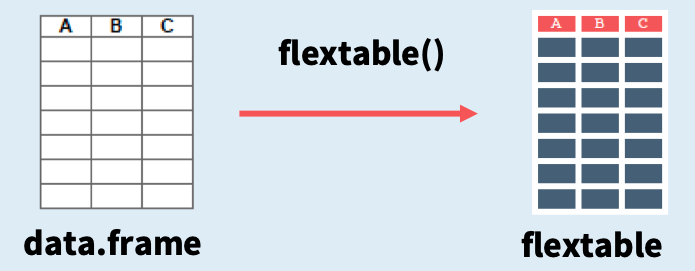
\includegraphics[width=9.65in]{images/flextab} \caption{Von data.frame zur Tabelle}\label{fig:unnamed-chunk-191}
\end{figure}

\begin{Shaded}
\begin{Highlighting}[]
\FunctionTok{library}\NormalTok{(flextable)}
\end{Highlighting}
\end{Shaded}

\begin{verbatim}
## 
## Attaching package: 'flextable'
\end{verbatim}

\begin{verbatim}
## The following objects are masked from 'package:ggpubr':
## 
##     border, font, rotate
\end{verbatim}

\begin{verbatim}
## The following object is masked from 'package:purrr':
## 
##     compose
\end{verbatim}

\begin{Shaded}
\begin{Highlighting}[]
\FunctionTok{flextable}\NormalTok{(df)}
\end{Highlighting}
\end{Shaded}

\providecommand{\docline}[3]{\noalign{\global\setlength{\arrayrulewidth}{#1}}\arrayrulecolor[HTML]{#2}\cline{#3}}

\setlength{\tabcolsep}{2pt}

\renewcommand*{\arraystretch}{1.5}

\begin{longtable}[c]{|p{0.75in}|p{0.75in}|p{0.75in}|p{0.75in}}



\hhline{>{\arrayrulecolor[HTML]{666666}\global\arrayrulewidth=2pt}->{\arrayrulecolor[HTML]{666666}\global\arrayrulewidth=2pt}->{\arrayrulecolor[HTML]{666666}\global\arrayrulewidth=2pt}->{\arrayrulecolor[HTML]{666666}\global\arrayrulewidth=2pt}-}

\multicolumn{1}{!{\color[HTML]{000000}\vrule width 0pt}>{\raggedright}p{\dimexpr 0.75in+0\tabcolsep+0\arrayrulewidth}}{\fontsize{11}{11}\selectfont{\textcolor[HTML]{000000}{\global\setmainfont{Helvetica}{Geschlecht}}}} & \multicolumn{1}{!{\color[HTML]{000000}\vrule width 0pt}>{\raggedleft}p{\dimexpr 0.75in+0\tabcolsep+0\arrayrulewidth}}{\fontsize{11}{11}\selectfont{\textcolor[HTML]{000000}{\global\setmainfont{Helvetica}{Konzentration}}}} & \multicolumn{1}{!{\color[HTML]{000000}\vrule width 0pt}>{\raggedleft}p{\dimexpr 0.75in+0\tabcolsep+0\arrayrulewidth}}{\fontsize{11}{11}\selectfont{\textcolor[HTML]{000000}{\global\setmainfont{Helvetica}{Schlafdauer}}}} & \multicolumn{1}{!{\color[HTML]{000000}\vrule width 0pt}>{\raggedleft}p{\dimexpr 0.75in+0\tabcolsep+0\arrayrulewidth}!{\color[HTML]{000000}\vrule width 0pt}}{\fontsize{11}{11}\selectfont{\textcolor[HTML]{000000}{\global\setmainfont{Helvetica}{Schlafqualität}}}} \\

\hhline{>{\arrayrulecolor[HTML]{666666}\global\arrayrulewidth=2pt}->{\arrayrulecolor[HTML]{666666}\global\arrayrulewidth=2pt}->{\arrayrulecolor[HTML]{666666}\global\arrayrulewidth=2pt}->{\arrayrulecolor[HTML]{666666}\global\arrayrulewidth=2pt}-}

\endfirsthead

\hhline{>{\arrayrulecolor[HTML]{666666}\global\arrayrulewidth=2pt}->{\arrayrulecolor[HTML]{666666}\global\arrayrulewidth=2pt}->{\arrayrulecolor[HTML]{666666}\global\arrayrulewidth=2pt}->{\arrayrulecolor[HTML]{666666}\global\arrayrulewidth=2pt}-}

\multicolumn{1}{!{\color[HTML]{000000}\vrule width 0pt}>{\raggedright}p{\dimexpr 0.75in+0\tabcolsep+0\arrayrulewidth}}{\fontsize{11}{11}\selectfont{\textcolor[HTML]{000000}{\global\setmainfont{Helvetica}{Geschlecht}}}} & \multicolumn{1}{!{\color[HTML]{000000}\vrule width 0pt}>{\raggedleft}p{\dimexpr 0.75in+0\tabcolsep+0\arrayrulewidth}}{\fontsize{11}{11}\selectfont{\textcolor[HTML]{000000}{\global\setmainfont{Helvetica}{Konzentration}}}} & \multicolumn{1}{!{\color[HTML]{000000}\vrule width 0pt}>{\raggedleft}p{\dimexpr 0.75in+0\tabcolsep+0\arrayrulewidth}}{\fontsize{11}{11}\selectfont{\textcolor[HTML]{000000}{\global\setmainfont{Helvetica}{Schlafdauer}}}} & \multicolumn{1}{!{\color[HTML]{000000}\vrule width 0pt}>{\raggedleft}p{\dimexpr 0.75in+0\tabcolsep+0\arrayrulewidth}!{\color[HTML]{000000}\vrule width 0pt}}{\fontsize{11}{11}\selectfont{\textcolor[HTML]{000000}{\global\setmainfont{Helvetica}{Schlafqualität}}}} \\

\hhline{>{\arrayrulecolor[HTML]{666666}\global\arrayrulewidth=2pt}->{\arrayrulecolor[HTML]{666666}\global\arrayrulewidth=2pt}->{\arrayrulecolor[HTML]{666666}\global\arrayrulewidth=2pt}->{\arrayrulecolor[HTML]{666666}\global\arrayrulewidth=2pt}-}\endhead



\multicolumn{1}{!{\color[HTML]{000000}\vrule width 0pt}>{\raggedright}p{\dimexpr 0.75in+0\tabcolsep+0\arrayrulewidth}}{\fontsize{11}{11}\selectfont{\textcolor[HTML]{000000}{\global\setmainfont{Helvetica}{männlich}}}} & \multicolumn{1}{!{\color[HTML]{000000}\vrule width 0pt}>{\raggedleft}p{\dimexpr 0.75in+0\tabcolsep+0\arrayrulewidth}}{\fontsize{11}{11}\selectfont{\textcolor[HTML]{000000}{\global\setmainfont{Helvetica}{3}}}} & \multicolumn{1}{!{\color[HTML]{000000}\vrule width 0pt}>{\raggedleft}p{\dimexpr 0.75in+0\tabcolsep+0\arrayrulewidth}}{\fontsize{11}{11}\selectfont{\textcolor[HTML]{000000}{\global\setmainfont{Helvetica}{6}}}} & \multicolumn{1}{!{\color[HTML]{000000}\vrule width 0pt}>{\raggedleft}p{\dimexpr 0.75in+0\tabcolsep+0\arrayrulewidth}!{\color[HTML]{000000}\vrule width 0pt}}{\fontsize{11}{11}\selectfont{\textcolor[HTML]{000000}{\global\setmainfont{Helvetica}{5}}}} \\





\multicolumn{1}{!{\color[HTML]{000000}\vrule width 0pt}>{\raggedright}p{\dimexpr 0.75in+0\tabcolsep+0\arrayrulewidth}}{\fontsize{11}{11}\selectfont{\textcolor[HTML]{000000}{\global\setmainfont{Helvetica}{männlich}}}} & \multicolumn{1}{!{\color[HTML]{000000}\vrule width 0pt}>{\raggedleft}p{\dimexpr 0.75in+0\tabcolsep+0\arrayrulewidth}}{\fontsize{11}{11}\selectfont{\textcolor[HTML]{000000}{\global\setmainfont{Helvetica}{7}}}} & \multicolumn{1}{!{\color[HTML]{000000}\vrule width 0pt}>{\raggedleft}p{\dimexpr 0.75in+0\tabcolsep+0\arrayrulewidth}}{\fontsize{11}{11}\selectfont{\textcolor[HTML]{000000}{\global\setmainfont{Helvetica}{14}}}} & \multicolumn{1}{!{\color[HTML]{000000}\vrule width 0pt}>{\raggedleft}p{\dimexpr 0.75in+0\tabcolsep+0\arrayrulewidth}!{\color[HTML]{000000}\vrule width 0pt}}{\fontsize{11}{11}\selectfont{\textcolor[HTML]{000000}{\global\setmainfont{Helvetica}{8}}}} \\





\multicolumn{1}{!{\color[HTML]{000000}\vrule width 0pt}>{\raggedright}p{\dimexpr 0.75in+0\tabcolsep+0\arrayrulewidth}}{\fontsize{11}{11}\selectfont{\textcolor[HTML]{000000}{\global\setmainfont{Helvetica}{weiblich}}}} & \multicolumn{1}{!{\color[HTML]{000000}\vrule width 0pt}>{\raggedleft}p{\dimexpr 0.75in+0\tabcolsep+0\arrayrulewidth}}{\fontsize{11}{11}\selectfont{\textcolor[HTML]{000000}{\global\setmainfont{Helvetica}{4}}}} & \multicolumn{1}{!{\color[HTML]{000000}\vrule width 0pt}>{\raggedleft}p{\dimexpr 0.75in+0\tabcolsep+0\arrayrulewidth}}{\fontsize{11}{11}\selectfont{\textcolor[HTML]{000000}{\global\setmainfont{Helvetica}{7}}}} & \multicolumn{1}{!{\color[HTML]{000000}\vrule width 0pt}>{\raggedleft}p{\dimexpr 0.75in+0\tabcolsep+0\arrayrulewidth}!{\color[HTML]{000000}\vrule width 0pt}}{\fontsize{11}{11}\selectfont{\textcolor[HTML]{000000}{\global\setmainfont{Helvetica}{2}}}} \\





\multicolumn{1}{!{\color[HTML]{000000}\vrule width 0pt}>{\raggedright}p{\dimexpr 0.75in+0\tabcolsep+0\arrayrulewidth}}{\fontsize{11}{11}\selectfont{\textcolor[HTML]{000000}{\global\setmainfont{Helvetica}{weiblich}}}} & \multicolumn{1}{!{\color[HTML]{000000}\vrule width 0pt}>{\raggedleft}p{\dimexpr 0.75in+0\tabcolsep+0\arrayrulewidth}}{\fontsize{11}{11}\selectfont{\textcolor[HTML]{000000}{\global\setmainfont{Helvetica}{7}}}} & \multicolumn{1}{!{\color[HTML]{000000}\vrule width 0pt}>{\raggedleft}p{\dimexpr 0.75in+0\tabcolsep+0\arrayrulewidth}}{\fontsize{11}{11}\selectfont{\textcolor[HTML]{000000}{\global\setmainfont{Helvetica}{12}}}} & \multicolumn{1}{!{\color[HTML]{000000}\vrule width 0pt}>{\raggedleft}p{\dimexpr 0.75in+0\tabcolsep+0\arrayrulewidth}!{\color[HTML]{000000}\vrule width 0pt}}{\fontsize{11}{11}\selectfont{\textcolor[HTML]{000000}{\global\setmainfont{Helvetica}{1}}}} \\

\hhline{>{\arrayrulecolor[HTML]{666666}\global\arrayrulewidth=2pt}->{\arrayrulecolor[HTML]{666666}\global\arrayrulewidth=2pt}->{\arrayrulecolor[HTML]{666666}\global\arrayrulewidth=2pt}->{\arrayrulecolor[HTML]{666666}\global\arrayrulewidth=2pt}-}



\end{longtable}

Die Bestandteile der Tabelle sind wie folgt:

\begin{figure}
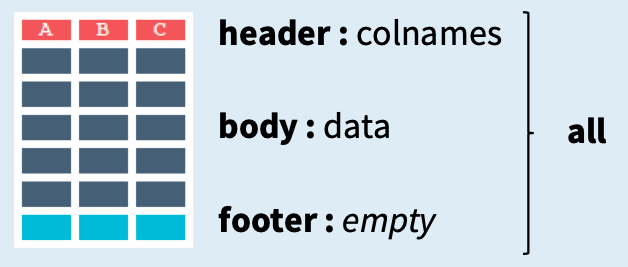
\includegraphics[width=8.72in]{images/flextab2} \caption{Bestandteile der Tabelle}\label{fig:unnamed-chunk-193}
\end{figure}

Der allgemeine Aufbau einer \texttt{flextable} Funktion lautet:

\texttt{function(x,\ i,\ j,\ part,\ args)}

\begin{itemize}
\tightlist
\item
  x = flextable Objekt (Ergebnis von \texttt{flextable()})
\item
  i = Zeilenindex
\item
  j = Spaltenindex,
\item
  part = Tabellenteil (header, body, footer)
\item
  args = spezielle weitere Anpassungen
\end{itemize}

\hypertarget{format}{%
\section{Format}\label{format}}

Es können diverse Aspekte der Tabelle angepasst werden.

\hypertarget{text}{%
\subsection{Text}\label{text}}

\hypertarget{fett-schreiben}{%
\subsubsection{Fett schreiben}\label{fett-schreiben}}

Zum Verwenden einer fetten Schriftart nutzen wir die \texttt{bold()} Funktion:

\begin{Shaded}
\begin{Highlighting}[]
\FunctionTok{bold}\NormalTok{(}\FunctionTok{flextable}\NormalTok{(df), }\AttributeTok{j =} \DecValTok{1}\NormalTok{, }\AttributeTok{bold =}\NormalTok{ T)}
\end{Highlighting}
\end{Shaded}

\providecommand{\docline}[3]{\noalign{\global\setlength{\arrayrulewidth}{#1}}\arrayrulecolor[HTML]{#2}\cline{#3}}

\setlength{\tabcolsep}{2pt}

\renewcommand*{\arraystretch}{1.5}

\begin{longtable}[c]{|p{0.75in}|p{0.75in}|p{0.75in}|p{0.75in}}



\hhline{>{\arrayrulecolor[HTML]{666666}\global\arrayrulewidth=2pt}->{\arrayrulecolor[HTML]{666666}\global\arrayrulewidth=2pt}->{\arrayrulecolor[HTML]{666666}\global\arrayrulewidth=2pt}->{\arrayrulecolor[HTML]{666666}\global\arrayrulewidth=2pt}-}

\multicolumn{1}{!{\color[HTML]{000000}\vrule width 0pt}>{\raggedright}p{\dimexpr 0.75in+0\tabcolsep+0\arrayrulewidth}}{\fontsize{11}{11}\selectfont{\textcolor[HTML]{000000}{\global\setmainfont{Helvetica}{Geschlecht}}}} & \multicolumn{1}{!{\color[HTML]{000000}\vrule width 0pt}>{\raggedleft}p{\dimexpr 0.75in+0\tabcolsep+0\arrayrulewidth}}{\fontsize{11}{11}\selectfont{\textcolor[HTML]{000000}{\global\setmainfont{Helvetica}{Konzentration}}}} & \multicolumn{1}{!{\color[HTML]{000000}\vrule width 0pt}>{\raggedleft}p{\dimexpr 0.75in+0\tabcolsep+0\arrayrulewidth}}{\fontsize{11}{11}\selectfont{\textcolor[HTML]{000000}{\global\setmainfont{Helvetica}{Schlafdauer}}}} & \multicolumn{1}{!{\color[HTML]{000000}\vrule width 0pt}>{\raggedleft}p{\dimexpr 0.75in+0\tabcolsep+0\arrayrulewidth}!{\color[HTML]{000000}\vrule width 0pt}}{\fontsize{11}{11}\selectfont{\textcolor[HTML]{000000}{\global\setmainfont{Helvetica}{Schlafqualität}}}} \\

\hhline{>{\arrayrulecolor[HTML]{666666}\global\arrayrulewidth=2pt}->{\arrayrulecolor[HTML]{666666}\global\arrayrulewidth=2pt}->{\arrayrulecolor[HTML]{666666}\global\arrayrulewidth=2pt}->{\arrayrulecolor[HTML]{666666}\global\arrayrulewidth=2pt}-}

\endfirsthead

\hhline{>{\arrayrulecolor[HTML]{666666}\global\arrayrulewidth=2pt}->{\arrayrulecolor[HTML]{666666}\global\arrayrulewidth=2pt}->{\arrayrulecolor[HTML]{666666}\global\arrayrulewidth=2pt}->{\arrayrulecolor[HTML]{666666}\global\arrayrulewidth=2pt}-}

\multicolumn{1}{!{\color[HTML]{000000}\vrule width 0pt}>{\raggedright}p{\dimexpr 0.75in+0\tabcolsep+0\arrayrulewidth}}{\fontsize{11}{11}\selectfont{\textcolor[HTML]{000000}{\global\setmainfont{Helvetica}{Geschlecht}}}} & \multicolumn{1}{!{\color[HTML]{000000}\vrule width 0pt}>{\raggedleft}p{\dimexpr 0.75in+0\tabcolsep+0\arrayrulewidth}}{\fontsize{11}{11}\selectfont{\textcolor[HTML]{000000}{\global\setmainfont{Helvetica}{Konzentration}}}} & \multicolumn{1}{!{\color[HTML]{000000}\vrule width 0pt}>{\raggedleft}p{\dimexpr 0.75in+0\tabcolsep+0\arrayrulewidth}}{\fontsize{11}{11}\selectfont{\textcolor[HTML]{000000}{\global\setmainfont{Helvetica}{Schlafdauer}}}} & \multicolumn{1}{!{\color[HTML]{000000}\vrule width 0pt}>{\raggedleft}p{\dimexpr 0.75in+0\tabcolsep+0\arrayrulewidth}!{\color[HTML]{000000}\vrule width 0pt}}{\fontsize{11}{11}\selectfont{\textcolor[HTML]{000000}{\global\setmainfont{Helvetica}{Schlafqualität}}}} \\

\hhline{>{\arrayrulecolor[HTML]{666666}\global\arrayrulewidth=2pt}->{\arrayrulecolor[HTML]{666666}\global\arrayrulewidth=2pt}->{\arrayrulecolor[HTML]{666666}\global\arrayrulewidth=2pt}->{\arrayrulecolor[HTML]{666666}\global\arrayrulewidth=2pt}-}\endhead



\multicolumn{1}{!{\color[HTML]{000000}\vrule width 0pt}>{\raggedright}p{\dimexpr 0.75in+0\tabcolsep+0\arrayrulewidth}}{\fontsize{11}{11}\selectfont{\textcolor[HTML]{000000}{\global\setmainfont{Helvetica}{\textbf{männlich}}}}} & \multicolumn{1}{!{\color[HTML]{000000}\vrule width 0pt}>{\raggedleft}p{\dimexpr 0.75in+0\tabcolsep+0\arrayrulewidth}}{\fontsize{11}{11}\selectfont{\textcolor[HTML]{000000}{\global\setmainfont{Helvetica}{3}}}} & \multicolumn{1}{!{\color[HTML]{000000}\vrule width 0pt}>{\raggedleft}p{\dimexpr 0.75in+0\tabcolsep+0\arrayrulewidth}}{\fontsize{11}{11}\selectfont{\textcolor[HTML]{000000}{\global\setmainfont{Helvetica}{6}}}} & \multicolumn{1}{!{\color[HTML]{000000}\vrule width 0pt}>{\raggedleft}p{\dimexpr 0.75in+0\tabcolsep+0\arrayrulewidth}!{\color[HTML]{000000}\vrule width 0pt}}{\fontsize{11}{11}\selectfont{\textcolor[HTML]{000000}{\global\setmainfont{Helvetica}{5}}}} \\





\multicolumn{1}{!{\color[HTML]{000000}\vrule width 0pt}>{\raggedright}p{\dimexpr 0.75in+0\tabcolsep+0\arrayrulewidth}}{\fontsize{11}{11}\selectfont{\textcolor[HTML]{000000}{\global\setmainfont{Helvetica}{\textbf{männlich}}}}} & \multicolumn{1}{!{\color[HTML]{000000}\vrule width 0pt}>{\raggedleft}p{\dimexpr 0.75in+0\tabcolsep+0\arrayrulewidth}}{\fontsize{11}{11}\selectfont{\textcolor[HTML]{000000}{\global\setmainfont{Helvetica}{7}}}} & \multicolumn{1}{!{\color[HTML]{000000}\vrule width 0pt}>{\raggedleft}p{\dimexpr 0.75in+0\tabcolsep+0\arrayrulewidth}}{\fontsize{11}{11}\selectfont{\textcolor[HTML]{000000}{\global\setmainfont{Helvetica}{14}}}} & \multicolumn{1}{!{\color[HTML]{000000}\vrule width 0pt}>{\raggedleft}p{\dimexpr 0.75in+0\tabcolsep+0\arrayrulewidth}!{\color[HTML]{000000}\vrule width 0pt}}{\fontsize{11}{11}\selectfont{\textcolor[HTML]{000000}{\global\setmainfont{Helvetica}{8}}}} \\





\multicolumn{1}{!{\color[HTML]{000000}\vrule width 0pt}>{\raggedright}p{\dimexpr 0.75in+0\tabcolsep+0\arrayrulewidth}}{\fontsize{11}{11}\selectfont{\textcolor[HTML]{000000}{\global\setmainfont{Helvetica}{\textbf{weiblich}}}}} & \multicolumn{1}{!{\color[HTML]{000000}\vrule width 0pt}>{\raggedleft}p{\dimexpr 0.75in+0\tabcolsep+0\arrayrulewidth}}{\fontsize{11}{11}\selectfont{\textcolor[HTML]{000000}{\global\setmainfont{Helvetica}{4}}}} & \multicolumn{1}{!{\color[HTML]{000000}\vrule width 0pt}>{\raggedleft}p{\dimexpr 0.75in+0\tabcolsep+0\arrayrulewidth}}{\fontsize{11}{11}\selectfont{\textcolor[HTML]{000000}{\global\setmainfont{Helvetica}{7}}}} & \multicolumn{1}{!{\color[HTML]{000000}\vrule width 0pt}>{\raggedleft}p{\dimexpr 0.75in+0\tabcolsep+0\arrayrulewidth}!{\color[HTML]{000000}\vrule width 0pt}}{\fontsize{11}{11}\selectfont{\textcolor[HTML]{000000}{\global\setmainfont{Helvetica}{2}}}} \\





\multicolumn{1}{!{\color[HTML]{000000}\vrule width 0pt}>{\raggedright}p{\dimexpr 0.75in+0\tabcolsep+0\arrayrulewidth}}{\fontsize{11}{11}\selectfont{\textcolor[HTML]{000000}{\global\setmainfont{Helvetica}{\textbf{weiblich}}}}} & \multicolumn{1}{!{\color[HTML]{000000}\vrule width 0pt}>{\raggedleft}p{\dimexpr 0.75in+0\tabcolsep+0\arrayrulewidth}}{\fontsize{11}{11}\selectfont{\textcolor[HTML]{000000}{\global\setmainfont{Helvetica}{7}}}} & \multicolumn{1}{!{\color[HTML]{000000}\vrule width 0pt}>{\raggedleft}p{\dimexpr 0.75in+0\tabcolsep+0\arrayrulewidth}}{\fontsize{11}{11}\selectfont{\textcolor[HTML]{000000}{\global\setmainfont{Helvetica}{12}}}} & \multicolumn{1}{!{\color[HTML]{000000}\vrule width 0pt}>{\raggedleft}p{\dimexpr 0.75in+0\tabcolsep+0\arrayrulewidth}!{\color[HTML]{000000}\vrule width 0pt}}{\fontsize{11}{11}\selectfont{\textcolor[HTML]{000000}{\global\setmainfont{Helvetica}{1}}}} \\

\hhline{>{\arrayrulecolor[HTML]{666666}\global\arrayrulewidth=2pt}->{\arrayrulecolor[HTML]{666666}\global\arrayrulewidth=2pt}->{\arrayrulecolor[HTML]{666666}\global\arrayrulewidth=2pt}->{\arrayrulecolor[HTML]{666666}\global\arrayrulewidth=2pt}-}



\end{longtable}

\hypertarget{kursiv-schreiben}{%
\subsubsection{Kursiv schreiben}\label{kursiv-schreiben}}

Zum Verwenden einer kursiven Schriftart nutzen wir die \texttt{italic()} Funktion:

\begin{Shaded}
\begin{Highlighting}[]
\FunctionTok{italic}\NormalTok{(}\FunctionTok{flextable}\NormalTok{(df), }\AttributeTok{j =} \DecValTok{1}\NormalTok{, }\AttributeTok{italic =}\NormalTok{ T)}
\end{Highlighting}
\end{Shaded}

\providecommand{\docline}[3]{\noalign{\global\setlength{\arrayrulewidth}{#1}}\arrayrulecolor[HTML]{#2}\cline{#3}}

\setlength{\tabcolsep}{2pt}

\renewcommand*{\arraystretch}{1.5}

\begin{longtable}[c]{|p{0.75in}|p{0.75in}|p{0.75in}|p{0.75in}}



\hhline{>{\arrayrulecolor[HTML]{666666}\global\arrayrulewidth=2pt}->{\arrayrulecolor[HTML]{666666}\global\arrayrulewidth=2pt}->{\arrayrulecolor[HTML]{666666}\global\arrayrulewidth=2pt}->{\arrayrulecolor[HTML]{666666}\global\arrayrulewidth=2pt}-}

\multicolumn{1}{!{\color[HTML]{000000}\vrule width 0pt}>{\raggedright}p{\dimexpr 0.75in+0\tabcolsep+0\arrayrulewidth}}{\fontsize{11}{11}\selectfont{\textcolor[HTML]{000000}{\global\setmainfont{Helvetica}{Geschlecht}}}} & \multicolumn{1}{!{\color[HTML]{000000}\vrule width 0pt}>{\raggedleft}p{\dimexpr 0.75in+0\tabcolsep+0\arrayrulewidth}}{\fontsize{11}{11}\selectfont{\textcolor[HTML]{000000}{\global\setmainfont{Helvetica}{Konzentration}}}} & \multicolumn{1}{!{\color[HTML]{000000}\vrule width 0pt}>{\raggedleft}p{\dimexpr 0.75in+0\tabcolsep+0\arrayrulewidth}}{\fontsize{11}{11}\selectfont{\textcolor[HTML]{000000}{\global\setmainfont{Helvetica}{Schlafdauer}}}} & \multicolumn{1}{!{\color[HTML]{000000}\vrule width 0pt}>{\raggedleft}p{\dimexpr 0.75in+0\tabcolsep+0\arrayrulewidth}!{\color[HTML]{000000}\vrule width 0pt}}{\fontsize{11}{11}\selectfont{\textcolor[HTML]{000000}{\global\setmainfont{Helvetica}{Schlafqualität}}}} \\

\hhline{>{\arrayrulecolor[HTML]{666666}\global\arrayrulewidth=2pt}->{\arrayrulecolor[HTML]{666666}\global\arrayrulewidth=2pt}->{\arrayrulecolor[HTML]{666666}\global\arrayrulewidth=2pt}->{\arrayrulecolor[HTML]{666666}\global\arrayrulewidth=2pt}-}

\endfirsthead

\hhline{>{\arrayrulecolor[HTML]{666666}\global\arrayrulewidth=2pt}->{\arrayrulecolor[HTML]{666666}\global\arrayrulewidth=2pt}->{\arrayrulecolor[HTML]{666666}\global\arrayrulewidth=2pt}->{\arrayrulecolor[HTML]{666666}\global\arrayrulewidth=2pt}-}

\multicolumn{1}{!{\color[HTML]{000000}\vrule width 0pt}>{\raggedright}p{\dimexpr 0.75in+0\tabcolsep+0\arrayrulewidth}}{\fontsize{11}{11}\selectfont{\textcolor[HTML]{000000}{\global\setmainfont{Helvetica}{Geschlecht}}}} & \multicolumn{1}{!{\color[HTML]{000000}\vrule width 0pt}>{\raggedleft}p{\dimexpr 0.75in+0\tabcolsep+0\arrayrulewidth}}{\fontsize{11}{11}\selectfont{\textcolor[HTML]{000000}{\global\setmainfont{Helvetica}{Konzentration}}}} & \multicolumn{1}{!{\color[HTML]{000000}\vrule width 0pt}>{\raggedleft}p{\dimexpr 0.75in+0\tabcolsep+0\arrayrulewidth}}{\fontsize{11}{11}\selectfont{\textcolor[HTML]{000000}{\global\setmainfont{Helvetica}{Schlafdauer}}}} & \multicolumn{1}{!{\color[HTML]{000000}\vrule width 0pt}>{\raggedleft}p{\dimexpr 0.75in+0\tabcolsep+0\arrayrulewidth}!{\color[HTML]{000000}\vrule width 0pt}}{\fontsize{11}{11}\selectfont{\textcolor[HTML]{000000}{\global\setmainfont{Helvetica}{Schlafqualität}}}} \\

\hhline{>{\arrayrulecolor[HTML]{666666}\global\arrayrulewidth=2pt}->{\arrayrulecolor[HTML]{666666}\global\arrayrulewidth=2pt}->{\arrayrulecolor[HTML]{666666}\global\arrayrulewidth=2pt}->{\arrayrulecolor[HTML]{666666}\global\arrayrulewidth=2pt}-}\endhead



\multicolumn{1}{!{\color[HTML]{000000}\vrule width 0pt}>{\raggedright}p{\dimexpr 0.75in+0\tabcolsep+0\arrayrulewidth}}{\fontsize{11}{11}\selectfont{\textcolor[HTML]{000000}{\global\setmainfont{Helvetica}{\textit{männlich}}}}} & \multicolumn{1}{!{\color[HTML]{000000}\vrule width 0pt}>{\raggedleft}p{\dimexpr 0.75in+0\tabcolsep+0\arrayrulewidth}}{\fontsize{11}{11}\selectfont{\textcolor[HTML]{000000}{\global\setmainfont{Helvetica}{3}}}} & \multicolumn{1}{!{\color[HTML]{000000}\vrule width 0pt}>{\raggedleft}p{\dimexpr 0.75in+0\tabcolsep+0\arrayrulewidth}}{\fontsize{11}{11}\selectfont{\textcolor[HTML]{000000}{\global\setmainfont{Helvetica}{6}}}} & \multicolumn{1}{!{\color[HTML]{000000}\vrule width 0pt}>{\raggedleft}p{\dimexpr 0.75in+0\tabcolsep+0\arrayrulewidth}!{\color[HTML]{000000}\vrule width 0pt}}{\fontsize{11}{11}\selectfont{\textcolor[HTML]{000000}{\global\setmainfont{Helvetica}{5}}}} \\





\multicolumn{1}{!{\color[HTML]{000000}\vrule width 0pt}>{\raggedright}p{\dimexpr 0.75in+0\tabcolsep+0\arrayrulewidth}}{\fontsize{11}{11}\selectfont{\textcolor[HTML]{000000}{\global\setmainfont{Helvetica}{\textit{männlich}}}}} & \multicolumn{1}{!{\color[HTML]{000000}\vrule width 0pt}>{\raggedleft}p{\dimexpr 0.75in+0\tabcolsep+0\arrayrulewidth}}{\fontsize{11}{11}\selectfont{\textcolor[HTML]{000000}{\global\setmainfont{Helvetica}{7}}}} & \multicolumn{1}{!{\color[HTML]{000000}\vrule width 0pt}>{\raggedleft}p{\dimexpr 0.75in+0\tabcolsep+0\arrayrulewidth}}{\fontsize{11}{11}\selectfont{\textcolor[HTML]{000000}{\global\setmainfont{Helvetica}{14}}}} & \multicolumn{1}{!{\color[HTML]{000000}\vrule width 0pt}>{\raggedleft}p{\dimexpr 0.75in+0\tabcolsep+0\arrayrulewidth}!{\color[HTML]{000000}\vrule width 0pt}}{\fontsize{11}{11}\selectfont{\textcolor[HTML]{000000}{\global\setmainfont{Helvetica}{8}}}} \\





\multicolumn{1}{!{\color[HTML]{000000}\vrule width 0pt}>{\raggedright}p{\dimexpr 0.75in+0\tabcolsep+0\arrayrulewidth}}{\fontsize{11}{11}\selectfont{\textcolor[HTML]{000000}{\global\setmainfont{Helvetica}{\textit{weiblich}}}}} & \multicolumn{1}{!{\color[HTML]{000000}\vrule width 0pt}>{\raggedleft}p{\dimexpr 0.75in+0\tabcolsep+0\arrayrulewidth}}{\fontsize{11}{11}\selectfont{\textcolor[HTML]{000000}{\global\setmainfont{Helvetica}{4}}}} & \multicolumn{1}{!{\color[HTML]{000000}\vrule width 0pt}>{\raggedleft}p{\dimexpr 0.75in+0\tabcolsep+0\arrayrulewidth}}{\fontsize{11}{11}\selectfont{\textcolor[HTML]{000000}{\global\setmainfont{Helvetica}{7}}}} & \multicolumn{1}{!{\color[HTML]{000000}\vrule width 0pt}>{\raggedleft}p{\dimexpr 0.75in+0\tabcolsep+0\arrayrulewidth}!{\color[HTML]{000000}\vrule width 0pt}}{\fontsize{11}{11}\selectfont{\textcolor[HTML]{000000}{\global\setmainfont{Helvetica}{2}}}} \\





\multicolumn{1}{!{\color[HTML]{000000}\vrule width 0pt}>{\raggedright}p{\dimexpr 0.75in+0\tabcolsep+0\arrayrulewidth}}{\fontsize{11}{11}\selectfont{\textcolor[HTML]{000000}{\global\setmainfont{Helvetica}{\textit{weiblich}}}}} & \multicolumn{1}{!{\color[HTML]{000000}\vrule width 0pt}>{\raggedleft}p{\dimexpr 0.75in+0\tabcolsep+0\arrayrulewidth}}{\fontsize{11}{11}\selectfont{\textcolor[HTML]{000000}{\global\setmainfont{Helvetica}{7}}}} & \multicolumn{1}{!{\color[HTML]{000000}\vrule width 0pt}>{\raggedleft}p{\dimexpr 0.75in+0\tabcolsep+0\arrayrulewidth}}{\fontsize{11}{11}\selectfont{\textcolor[HTML]{000000}{\global\setmainfont{Helvetica}{12}}}} & \multicolumn{1}{!{\color[HTML]{000000}\vrule width 0pt}>{\raggedleft}p{\dimexpr 0.75in+0\tabcolsep+0\arrayrulewidth}!{\color[HTML]{000000}\vrule width 0pt}}{\fontsize{11}{11}\selectfont{\textcolor[HTML]{000000}{\global\setmainfont{Helvetica}{1}}}} \\

\hhline{>{\arrayrulecolor[HTML]{666666}\global\arrayrulewidth=2pt}->{\arrayrulecolor[HTML]{666666}\global\arrayrulewidth=2pt}->{\arrayrulecolor[HTML]{666666}\global\arrayrulewidth=2pt}->{\arrayrulecolor[HTML]{666666}\global\arrayrulewidth=2pt}-}



\end{longtable}

\hypertarget{textgruxf6uxdfe-anpassen}{%
\subsubsection{Textgröße anpassen}\label{textgruxf6uxdfe-anpassen}}

Zur Veränderung der Textgröße nutzen wir die \texttt{fontsize()} Funktion:

\begin{Shaded}
\begin{Highlighting}[]
\FunctionTok{fontsize}\NormalTok{(}\FunctionTok{flextable}\NormalTok{(df), }\AttributeTok{j =} \DecValTok{1}\NormalTok{, }\AttributeTok{size =} \DecValTok{6}\NormalTok{)}
\end{Highlighting}
\end{Shaded}

\providecommand{\docline}[3]{\noalign{\global\setlength{\arrayrulewidth}{#1}}\arrayrulecolor[HTML]{#2}\cline{#3}}

\setlength{\tabcolsep}{2pt}

\renewcommand*{\arraystretch}{1.5}

\begin{longtable}[c]{|p{0.75in}|p{0.75in}|p{0.75in}|p{0.75in}}



\hhline{>{\arrayrulecolor[HTML]{666666}\global\arrayrulewidth=2pt}->{\arrayrulecolor[HTML]{666666}\global\arrayrulewidth=2pt}->{\arrayrulecolor[HTML]{666666}\global\arrayrulewidth=2pt}->{\arrayrulecolor[HTML]{666666}\global\arrayrulewidth=2pt}-}

\multicolumn{1}{!{\color[HTML]{000000}\vrule width 0pt}>{\raggedright}p{\dimexpr 0.75in+0\tabcolsep+0\arrayrulewidth}}{\fontsize{11}{11}\selectfont{\textcolor[HTML]{000000}{\global\setmainfont{Helvetica}{Geschlecht}}}} & \multicolumn{1}{!{\color[HTML]{000000}\vrule width 0pt}>{\raggedleft}p{\dimexpr 0.75in+0\tabcolsep+0\arrayrulewidth}}{\fontsize{11}{11}\selectfont{\textcolor[HTML]{000000}{\global\setmainfont{Helvetica}{Konzentration}}}} & \multicolumn{1}{!{\color[HTML]{000000}\vrule width 0pt}>{\raggedleft}p{\dimexpr 0.75in+0\tabcolsep+0\arrayrulewidth}}{\fontsize{11}{11}\selectfont{\textcolor[HTML]{000000}{\global\setmainfont{Helvetica}{Schlafdauer}}}} & \multicolumn{1}{!{\color[HTML]{000000}\vrule width 0pt}>{\raggedleft}p{\dimexpr 0.75in+0\tabcolsep+0\arrayrulewidth}!{\color[HTML]{000000}\vrule width 0pt}}{\fontsize{11}{11}\selectfont{\textcolor[HTML]{000000}{\global\setmainfont{Helvetica}{Schlafqualität}}}} \\

\hhline{>{\arrayrulecolor[HTML]{666666}\global\arrayrulewidth=2pt}->{\arrayrulecolor[HTML]{666666}\global\arrayrulewidth=2pt}->{\arrayrulecolor[HTML]{666666}\global\arrayrulewidth=2pt}->{\arrayrulecolor[HTML]{666666}\global\arrayrulewidth=2pt}-}

\endfirsthead

\hhline{>{\arrayrulecolor[HTML]{666666}\global\arrayrulewidth=2pt}->{\arrayrulecolor[HTML]{666666}\global\arrayrulewidth=2pt}->{\arrayrulecolor[HTML]{666666}\global\arrayrulewidth=2pt}->{\arrayrulecolor[HTML]{666666}\global\arrayrulewidth=2pt}-}

\multicolumn{1}{!{\color[HTML]{000000}\vrule width 0pt}>{\raggedright}p{\dimexpr 0.75in+0\tabcolsep+0\arrayrulewidth}}{\fontsize{11}{11}\selectfont{\textcolor[HTML]{000000}{\global\setmainfont{Helvetica}{Geschlecht}}}} & \multicolumn{1}{!{\color[HTML]{000000}\vrule width 0pt}>{\raggedleft}p{\dimexpr 0.75in+0\tabcolsep+0\arrayrulewidth}}{\fontsize{11}{11}\selectfont{\textcolor[HTML]{000000}{\global\setmainfont{Helvetica}{Konzentration}}}} & \multicolumn{1}{!{\color[HTML]{000000}\vrule width 0pt}>{\raggedleft}p{\dimexpr 0.75in+0\tabcolsep+0\arrayrulewidth}}{\fontsize{11}{11}\selectfont{\textcolor[HTML]{000000}{\global\setmainfont{Helvetica}{Schlafdauer}}}} & \multicolumn{1}{!{\color[HTML]{000000}\vrule width 0pt}>{\raggedleft}p{\dimexpr 0.75in+0\tabcolsep+0\arrayrulewidth}!{\color[HTML]{000000}\vrule width 0pt}}{\fontsize{11}{11}\selectfont{\textcolor[HTML]{000000}{\global\setmainfont{Helvetica}{Schlafqualität}}}} \\

\hhline{>{\arrayrulecolor[HTML]{666666}\global\arrayrulewidth=2pt}->{\arrayrulecolor[HTML]{666666}\global\arrayrulewidth=2pt}->{\arrayrulecolor[HTML]{666666}\global\arrayrulewidth=2pt}->{\arrayrulecolor[HTML]{666666}\global\arrayrulewidth=2pt}-}\endhead



\multicolumn{1}{!{\color[HTML]{000000}\vrule width 0pt}>{\raggedright}p{\dimexpr 0.75in+0\tabcolsep+0\arrayrulewidth}}{\fontsize{6}{6}\selectfont{\textcolor[HTML]{000000}{\global\setmainfont{Helvetica}{männlich}}}} & \multicolumn{1}{!{\color[HTML]{000000}\vrule width 0pt}>{\raggedleft}p{\dimexpr 0.75in+0\tabcolsep+0\arrayrulewidth}}{\fontsize{11}{11}\selectfont{\textcolor[HTML]{000000}{\global\setmainfont{Helvetica}{3}}}} & \multicolumn{1}{!{\color[HTML]{000000}\vrule width 0pt}>{\raggedleft}p{\dimexpr 0.75in+0\tabcolsep+0\arrayrulewidth}}{\fontsize{11}{11}\selectfont{\textcolor[HTML]{000000}{\global\setmainfont{Helvetica}{6}}}} & \multicolumn{1}{!{\color[HTML]{000000}\vrule width 0pt}>{\raggedleft}p{\dimexpr 0.75in+0\tabcolsep+0\arrayrulewidth}!{\color[HTML]{000000}\vrule width 0pt}}{\fontsize{11}{11}\selectfont{\textcolor[HTML]{000000}{\global\setmainfont{Helvetica}{5}}}} \\





\multicolumn{1}{!{\color[HTML]{000000}\vrule width 0pt}>{\raggedright}p{\dimexpr 0.75in+0\tabcolsep+0\arrayrulewidth}}{\fontsize{6}{6}\selectfont{\textcolor[HTML]{000000}{\global\setmainfont{Helvetica}{männlich}}}} & \multicolumn{1}{!{\color[HTML]{000000}\vrule width 0pt}>{\raggedleft}p{\dimexpr 0.75in+0\tabcolsep+0\arrayrulewidth}}{\fontsize{11}{11}\selectfont{\textcolor[HTML]{000000}{\global\setmainfont{Helvetica}{7}}}} & \multicolumn{1}{!{\color[HTML]{000000}\vrule width 0pt}>{\raggedleft}p{\dimexpr 0.75in+0\tabcolsep+0\arrayrulewidth}}{\fontsize{11}{11}\selectfont{\textcolor[HTML]{000000}{\global\setmainfont{Helvetica}{14}}}} & \multicolumn{1}{!{\color[HTML]{000000}\vrule width 0pt}>{\raggedleft}p{\dimexpr 0.75in+0\tabcolsep+0\arrayrulewidth}!{\color[HTML]{000000}\vrule width 0pt}}{\fontsize{11}{11}\selectfont{\textcolor[HTML]{000000}{\global\setmainfont{Helvetica}{8}}}} \\





\multicolumn{1}{!{\color[HTML]{000000}\vrule width 0pt}>{\raggedright}p{\dimexpr 0.75in+0\tabcolsep+0\arrayrulewidth}}{\fontsize{6}{6}\selectfont{\textcolor[HTML]{000000}{\global\setmainfont{Helvetica}{weiblich}}}} & \multicolumn{1}{!{\color[HTML]{000000}\vrule width 0pt}>{\raggedleft}p{\dimexpr 0.75in+0\tabcolsep+0\arrayrulewidth}}{\fontsize{11}{11}\selectfont{\textcolor[HTML]{000000}{\global\setmainfont{Helvetica}{4}}}} & \multicolumn{1}{!{\color[HTML]{000000}\vrule width 0pt}>{\raggedleft}p{\dimexpr 0.75in+0\tabcolsep+0\arrayrulewidth}}{\fontsize{11}{11}\selectfont{\textcolor[HTML]{000000}{\global\setmainfont{Helvetica}{7}}}} & \multicolumn{1}{!{\color[HTML]{000000}\vrule width 0pt}>{\raggedleft}p{\dimexpr 0.75in+0\tabcolsep+0\arrayrulewidth}!{\color[HTML]{000000}\vrule width 0pt}}{\fontsize{11}{11}\selectfont{\textcolor[HTML]{000000}{\global\setmainfont{Helvetica}{2}}}} \\





\multicolumn{1}{!{\color[HTML]{000000}\vrule width 0pt}>{\raggedright}p{\dimexpr 0.75in+0\tabcolsep+0\arrayrulewidth}}{\fontsize{6}{6}\selectfont{\textcolor[HTML]{000000}{\global\setmainfont{Helvetica}{weiblich}}}} & \multicolumn{1}{!{\color[HTML]{000000}\vrule width 0pt}>{\raggedleft}p{\dimexpr 0.75in+0\tabcolsep+0\arrayrulewidth}}{\fontsize{11}{11}\selectfont{\textcolor[HTML]{000000}{\global\setmainfont{Helvetica}{7}}}} & \multicolumn{1}{!{\color[HTML]{000000}\vrule width 0pt}>{\raggedleft}p{\dimexpr 0.75in+0\tabcolsep+0\arrayrulewidth}}{\fontsize{11}{11}\selectfont{\textcolor[HTML]{000000}{\global\setmainfont{Helvetica}{12}}}} & \multicolumn{1}{!{\color[HTML]{000000}\vrule width 0pt}>{\raggedleft}p{\dimexpr 0.75in+0\tabcolsep+0\arrayrulewidth}!{\color[HTML]{000000}\vrule width 0pt}}{\fontsize{11}{11}\selectfont{\textcolor[HTML]{000000}{\global\setmainfont{Helvetica}{1}}}} \\

\hhline{>{\arrayrulecolor[HTML]{666666}\global\arrayrulewidth=2pt}->{\arrayrulecolor[HTML]{666666}\global\arrayrulewidth=2pt}->{\arrayrulecolor[HTML]{666666}\global\arrayrulewidth=2pt}->{\arrayrulecolor[HTML]{666666}\global\arrayrulewidth=2pt}-}



\end{longtable}

\hypertarget{textfarbe-anpassen}{%
\subsubsection{Textfarbe anpassen}\label{textfarbe-anpassen}}

Zur Veränderung der Textfarbe nutzen wir die \texttt{color()} Funktion:

\begin{Shaded}
\begin{Highlighting}[]
\FunctionTok{color}\NormalTok{(}\FunctionTok{flextable}\NormalTok{(df), }\AttributeTok{j =} \DecValTok{1}\NormalTok{, }\AttributeTok{color =} \StringTok{"red"}\NormalTok{)}
\end{Highlighting}
\end{Shaded}

\providecommand{\docline}[3]{\noalign{\global\setlength{\arrayrulewidth}{#1}}\arrayrulecolor[HTML]{#2}\cline{#3}}

\setlength{\tabcolsep}{2pt}

\renewcommand*{\arraystretch}{1.5}

\begin{longtable}[c]{|p{0.75in}|p{0.75in}|p{0.75in}|p{0.75in}}



\hhline{>{\arrayrulecolor[HTML]{666666}\global\arrayrulewidth=2pt}->{\arrayrulecolor[HTML]{666666}\global\arrayrulewidth=2pt}->{\arrayrulecolor[HTML]{666666}\global\arrayrulewidth=2pt}->{\arrayrulecolor[HTML]{666666}\global\arrayrulewidth=2pt}-}

\multicolumn{1}{!{\color[HTML]{000000}\vrule width 0pt}>{\raggedright}p{\dimexpr 0.75in+0\tabcolsep+0\arrayrulewidth}}{\fontsize{11}{11}\selectfont{\textcolor[HTML]{000000}{\global\setmainfont{Helvetica}{Geschlecht}}}} & \multicolumn{1}{!{\color[HTML]{000000}\vrule width 0pt}>{\raggedleft}p{\dimexpr 0.75in+0\tabcolsep+0\arrayrulewidth}}{\fontsize{11}{11}\selectfont{\textcolor[HTML]{000000}{\global\setmainfont{Helvetica}{Konzentration}}}} & \multicolumn{1}{!{\color[HTML]{000000}\vrule width 0pt}>{\raggedleft}p{\dimexpr 0.75in+0\tabcolsep+0\arrayrulewidth}}{\fontsize{11}{11}\selectfont{\textcolor[HTML]{000000}{\global\setmainfont{Helvetica}{Schlafdauer}}}} & \multicolumn{1}{!{\color[HTML]{000000}\vrule width 0pt}>{\raggedleft}p{\dimexpr 0.75in+0\tabcolsep+0\arrayrulewidth}!{\color[HTML]{000000}\vrule width 0pt}}{\fontsize{11}{11}\selectfont{\textcolor[HTML]{000000}{\global\setmainfont{Helvetica}{Schlafqualität}}}} \\

\hhline{>{\arrayrulecolor[HTML]{666666}\global\arrayrulewidth=2pt}->{\arrayrulecolor[HTML]{666666}\global\arrayrulewidth=2pt}->{\arrayrulecolor[HTML]{666666}\global\arrayrulewidth=2pt}->{\arrayrulecolor[HTML]{666666}\global\arrayrulewidth=2pt}-}

\endfirsthead

\hhline{>{\arrayrulecolor[HTML]{666666}\global\arrayrulewidth=2pt}->{\arrayrulecolor[HTML]{666666}\global\arrayrulewidth=2pt}->{\arrayrulecolor[HTML]{666666}\global\arrayrulewidth=2pt}->{\arrayrulecolor[HTML]{666666}\global\arrayrulewidth=2pt}-}

\multicolumn{1}{!{\color[HTML]{000000}\vrule width 0pt}>{\raggedright}p{\dimexpr 0.75in+0\tabcolsep+0\arrayrulewidth}}{\fontsize{11}{11}\selectfont{\textcolor[HTML]{000000}{\global\setmainfont{Helvetica}{Geschlecht}}}} & \multicolumn{1}{!{\color[HTML]{000000}\vrule width 0pt}>{\raggedleft}p{\dimexpr 0.75in+0\tabcolsep+0\arrayrulewidth}}{\fontsize{11}{11}\selectfont{\textcolor[HTML]{000000}{\global\setmainfont{Helvetica}{Konzentration}}}} & \multicolumn{1}{!{\color[HTML]{000000}\vrule width 0pt}>{\raggedleft}p{\dimexpr 0.75in+0\tabcolsep+0\arrayrulewidth}}{\fontsize{11}{11}\selectfont{\textcolor[HTML]{000000}{\global\setmainfont{Helvetica}{Schlafdauer}}}} & \multicolumn{1}{!{\color[HTML]{000000}\vrule width 0pt}>{\raggedleft}p{\dimexpr 0.75in+0\tabcolsep+0\arrayrulewidth}!{\color[HTML]{000000}\vrule width 0pt}}{\fontsize{11}{11}\selectfont{\textcolor[HTML]{000000}{\global\setmainfont{Helvetica}{Schlafqualität}}}} \\

\hhline{>{\arrayrulecolor[HTML]{666666}\global\arrayrulewidth=2pt}->{\arrayrulecolor[HTML]{666666}\global\arrayrulewidth=2pt}->{\arrayrulecolor[HTML]{666666}\global\arrayrulewidth=2pt}->{\arrayrulecolor[HTML]{666666}\global\arrayrulewidth=2pt}-}\endhead



\multicolumn{1}{!{\color[HTML]{000000}\vrule width 0pt}>{\raggedright}p{\dimexpr 0.75in+0\tabcolsep+0\arrayrulewidth}}{\fontsize{11}{11}\selectfont{\textcolor[HTML]{FF0000}{\global\setmainfont{Helvetica}{männlich}}}} & \multicolumn{1}{!{\color[HTML]{000000}\vrule width 0pt}>{\raggedleft}p{\dimexpr 0.75in+0\tabcolsep+0\arrayrulewidth}}{\fontsize{11}{11}\selectfont{\textcolor[HTML]{000000}{\global\setmainfont{Helvetica}{3}}}} & \multicolumn{1}{!{\color[HTML]{000000}\vrule width 0pt}>{\raggedleft}p{\dimexpr 0.75in+0\tabcolsep+0\arrayrulewidth}}{\fontsize{11}{11}\selectfont{\textcolor[HTML]{000000}{\global\setmainfont{Helvetica}{6}}}} & \multicolumn{1}{!{\color[HTML]{000000}\vrule width 0pt}>{\raggedleft}p{\dimexpr 0.75in+0\tabcolsep+0\arrayrulewidth}!{\color[HTML]{000000}\vrule width 0pt}}{\fontsize{11}{11}\selectfont{\textcolor[HTML]{000000}{\global\setmainfont{Helvetica}{5}}}} \\





\multicolumn{1}{!{\color[HTML]{000000}\vrule width 0pt}>{\raggedright}p{\dimexpr 0.75in+0\tabcolsep+0\arrayrulewidth}}{\fontsize{11}{11}\selectfont{\textcolor[HTML]{FF0000}{\global\setmainfont{Helvetica}{männlich}}}} & \multicolumn{1}{!{\color[HTML]{000000}\vrule width 0pt}>{\raggedleft}p{\dimexpr 0.75in+0\tabcolsep+0\arrayrulewidth}}{\fontsize{11}{11}\selectfont{\textcolor[HTML]{000000}{\global\setmainfont{Helvetica}{7}}}} & \multicolumn{1}{!{\color[HTML]{000000}\vrule width 0pt}>{\raggedleft}p{\dimexpr 0.75in+0\tabcolsep+0\arrayrulewidth}}{\fontsize{11}{11}\selectfont{\textcolor[HTML]{000000}{\global\setmainfont{Helvetica}{14}}}} & \multicolumn{1}{!{\color[HTML]{000000}\vrule width 0pt}>{\raggedleft}p{\dimexpr 0.75in+0\tabcolsep+0\arrayrulewidth}!{\color[HTML]{000000}\vrule width 0pt}}{\fontsize{11}{11}\selectfont{\textcolor[HTML]{000000}{\global\setmainfont{Helvetica}{8}}}} \\





\multicolumn{1}{!{\color[HTML]{000000}\vrule width 0pt}>{\raggedright}p{\dimexpr 0.75in+0\tabcolsep+0\arrayrulewidth}}{\fontsize{11}{11}\selectfont{\textcolor[HTML]{FF0000}{\global\setmainfont{Helvetica}{weiblich}}}} & \multicolumn{1}{!{\color[HTML]{000000}\vrule width 0pt}>{\raggedleft}p{\dimexpr 0.75in+0\tabcolsep+0\arrayrulewidth}}{\fontsize{11}{11}\selectfont{\textcolor[HTML]{000000}{\global\setmainfont{Helvetica}{4}}}} & \multicolumn{1}{!{\color[HTML]{000000}\vrule width 0pt}>{\raggedleft}p{\dimexpr 0.75in+0\tabcolsep+0\arrayrulewidth}}{\fontsize{11}{11}\selectfont{\textcolor[HTML]{000000}{\global\setmainfont{Helvetica}{7}}}} & \multicolumn{1}{!{\color[HTML]{000000}\vrule width 0pt}>{\raggedleft}p{\dimexpr 0.75in+0\tabcolsep+0\arrayrulewidth}!{\color[HTML]{000000}\vrule width 0pt}}{\fontsize{11}{11}\selectfont{\textcolor[HTML]{000000}{\global\setmainfont{Helvetica}{2}}}} \\





\multicolumn{1}{!{\color[HTML]{000000}\vrule width 0pt}>{\raggedright}p{\dimexpr 0.75in+0\tabcolsep+0\arrayrulewidth}}{\fontsize{11}{11}\selectfont{\textcolor[HTML]{FF0000}{\global\setmainfont{Helvetica}{weiblich}}}} & \multicolumn{1}{!{\color[HTML]{000000}\vrule width 0pt}>{\raggedleft}p{\dimexpr 0.75in+0\tabcolsep+0\arrayrulewidth}}{\fontsize{11}{11}\selectfont{\textcolor[HTML]{000000}{\global\setmainfont{Helvetica}{7}}}} & \multicolumn{1}{!{\color[HTML]{000000}\vrule width 0pt}>{\raggedleft}p{\dimexpr 0.75in+0\tabcolsep+0\arrayrulewidth}}{\fontsize{11}{11}\selectfont{\textcolor[HTML]{000000}{\global\setmainfont{Helvetica}{12}}}} & \multicolumn{1}{!{\color[HTML]{000000}\vrule width 0pt}>{\raggedleft}p{\dimexpr 0.75in+0\tabcolsep+0\arrayrulewidth}!{\color[HTML]{000000}\vrule width 0pt}}{\fontsize{11}{11}\selectfont{\textcolor[HTML]{000000}{\global\setmainfont{Helvetica}{1}}}} \\

\hhline{>{\arrayrulecolor[HTML]{666666}\global\arrayrulewidth=2pt}->{\arrayrulecolor[HTML]{666666}\global\arrayrulewidth=2pt}->{\arrayrulecolor[HTML]{666666}\global\arrayrulewidth=2pt}->{\arrayrulecolor[HTML]{666666}\global\arrayrulewidth=2pt}-}



\end{longtable}

\hypertarget{text-hervorheben}{%
\subsubsection{Text hervorheben}\label{text-hervorheben}}

Zum Hervorheben von Text nutzen wir die \texttt{highlight()} Funktion:

\begin{Shaded}
\begin{Highlighting}[]
\FunctionTok{highlight}\NormalTok{(}\FunctionTok{flextable}\NormalTok{(df), }\AttributeTok{j =} \DecValTok{1}\NormalTok{, }\AttributeTok{color =} \StringTok{"yellow"}\NormalTok{)}
\end{Highlighting}
\end{Shaded}

\providecommand{\docline}[3]{\noalign{\global\setlength{\arrayrulewidth}{#1}}\arrayrulecolor[HTML]{#2}\cline{#3}}

\setlength{\tabcolsep}{2pt}

\renewcommand*{\arraystretch}{1.5}

\begin{longtable}[c]{|p{0.75in}|p{0.75in}|p{0.75in}|p{0.75in}}



\hhline{>{\arrayrulecolor[HTML]{666666}\global\arrayrulewidth=2pt}->{\arrayrulecolor[HTML]{666666}\global\arrayrulewidth=2pt}->{\arrayrulecolor[HTML]{666666}\global\arrayrulewidth=2pt}->{\arrayrulecolor[HTML]{666666}\global\arrayrulewidth=2pt}-}

\multicolumn{1}{!{\color[HTML]{000000}\vrule width 0pt}>{\raggedright}p{\dimexpr 0.75in+0\tabcolsep+0\arrayrulewidth}}{\fontsize{11}{11}\selectfont{\textcolor[HTML]{000000}{\global\setmainfont{Helvetica}{Geschlecht}}}} & \multicolumn{1}{!{\color[HTML]{000000}\vrule width 0pt}>{\raggedleft}p{\dimexpr 0.75in+0\tabcolsep+0\arrayrulewidth}}{\fontsize{11}{11}\selectfont{\textcolor[HTML]{000000}{\global\setmainfont{Helvetica}{Konzentration}}}} & \multicolumn{1}{!{\color[HTML]{000000}\vrule width 0pt}>{\raggedleft}p{\dimexpr 0.75in+0\tabcolsep+0\arrayrulewidth}}{\fontsize{11}{11}\selectfont{\textcolor[HTML]{000000}{\global\setmainfont{Helvetica}{Schlafdauer}}}} & \multicolumn{1}{!{\color[HTML]{000000}\vrule width 0pt}>{\raggedleft}p{\dimexpr 0.75in+0\tabcolsep+0\arrayrulewidth}!{\color[HTML]{000000}\vrule width 0pt}}{\fontsize{11}{11}\selectfont{\textcolor[HTML]{000000}{\global\setmainfont{Helvetica}{Schlafqualität}}}} \\

\hhline{>{\arrayrulecolor[HTML]{666666}\global\arrayrulewidth=2pt}->{\arrayrulecolor[HTML]{666666}\global\arrayrulewidth=2pt}->{\arrayrulecolor[HTML]{666666}\global\arrayrulewidth=2pt}->{\arrayrulecolor[HTML]{666666}\global\arrayrulewidth=2pt}-}

\endfirsthead

\hhline{>{\arrayrulecolor[HTML]{666666}\global\arrayrulewidth=2pt}->{\arrayrulecolor[HTML]{666666}\global\arrayrulewidth=2pt}->{\arrayrulecolor[HTML]{666666}\global\arrayrulewidth=2pt}->{\arrayrulecolor[HTML]{666666}\global\arrayrulewidth=2pt}-}

\multicolumn{1}{!{\color[HTML]{000000}\vrule width 0pt}>{\raggedright}p{\dimexpr 0.75in+0\tabcolsep+0\arrayrulewidth}}{\fontsize{11}{11}\selectfont{\textcolor[HTML]{000000}{\global\setmainfont{Helvetica}{Geschlecht}}}} & \multicolumn{1}{!{\color[HTML]{000000}\vrule width 0pt}>{\raggedleft}p{\dimexpr 0.75in+0\tabcolsep+0\arrayrulewidth}}{\fontsize{11}{11}\selectfont{\textcolor[HTML]{000000}{\global\setmainfont{Helvetica}{Konzentration}}}} & \multicolumn{1}{!{\color[HTML]{000000}\vrule width 0pt}>{\raggedleft}p{\dimexpr 0.75in+0\tabcolsep+0\arrayrulewidth}}{\fontsize{11}{11}\selectfont{\textcolor[HTML]{000000}{\global\setmainfont{Helvetica}{Schlafdauer}}}} & \multicolumn{1}{!{\color[HTML]{000000}\vrule width 0pt}>{\raggedleft}p{\dimexpr 0.75in+0\tabcolsep+0\arrayrulewidth}!{\color[HTML]{000000}\vrule width 0pt}}{\fontsize{11}{11}\selectfont{\textcolor[HTML]{000000}{\global\setmainfont{Helvetica}{Schlafqualität}}}} \\

\hhline{>{\arrayrulecolor[HTML]{666666}\global\arrayrulewidth=2pt}->{\arrayrulecolor[HTML]{666666}\global\arrayrulewidth=2pt}->{\arrayrulecolor[HTML]{666666}\global\arrayrulewidth=2pt}->{\arrayrulecolor[HTML]{666666}\global\arrayrulewidth=2pt}-}\endhead



\multicolumn{1}{!{\color[HTML]{000000}\vrule width 0pt}>{\raggedright}p{\dimexpr 0.75in+0\tabcolsep+0\arrayrulewidth}}{\fontsize{11}{11}\selectfont{\textcolor[HTML]{000000}{\colorbox[HTML]{FFFF00}{\global\setmainfont{Helvetica}{männlich}}}}} & \multicolumn{1}{!{\color[HTML]{000000}\vrule width 0pt}>{\raggedleft}p{\dimexpr 0.75in+0\tabcolsep+0\arrayrulewidth}}{\fontsize{11}{11}\selectfont{\textcolor[HTML]{000000}{\global\setmainfont{Helvetica}{3}}}} & \multicolumn{1}{!{\color[HTML]{000000}\vrule width 0pt}>{\raggedleft}p{\dimexpr 0.75in+0\tabcolsep+0\arrayrulewidth}}{\fontsize{11}{11}\selectfont{\textcolor[HTML]{000000}{\global\setmainfont{Helvetica}{6}}}} & \multicolumn{1}{!{\color[HTML]{000000}\vrule width 0pt}>{\raggedleft}p{\dimexpr 0.75in+0\tabcolsep+0\arrayrulewidth}!{\color[HTML]{000000}\vrule width 0pt}}{\fontsize{11}{11}\selectfont{\textcolor[HTML]{000000}{\global\setmainfont{Helvetica}{5}}}} \\





\multicolumn{1}{!{\color[HTML]{000000}\vrule width 0pt}>{\raggedright}p{\dimexpr 0.75in+0\tabcolsep+0\arrayrulewidth}}{\fontsize{11}{11}\selectfont{\textcolor[HTML]{000000}{\colorbox[HTML]{FFFF00}{\global\setmainfont{Helvetica}{männlich}}}}} & \multicolumn{1}{!{\color[HTML]{000000}\vrule width 0pt}>{\raggedleft}p{\dimexpr 0.75in+0\tabcolsep+0\arrayrulewidth}}{\fontsize{11}{11}\selectfont{\textcolor[HTML]{000000}{\global\setmainfont{Helvetica}{7}}}} & \multicolumn{1}{!{\color[HTML]{000000}\vrule width 0pt}>{\raggedleft}p{\dimexpr 0.75in+0\tabcolsep+0\arrayrulewidth}}{\fontsize{11}{11}\selectfont{\textcolor[HTML]{000000}{\global\setmainfont{Helvetica}{14}}}} & \multicolumn{1}{!{\color[HTML]{000000}\vrule width 0pt}>{\raggedleft}p{\dimexpr 0.75in+0\tabcolsep+0\arrayrulewidth}!{\color[HTML]{000000}\vrule width 0pt}}{\fontsize{11}{11}\selectfont{\textcolor[HTML]{000000}{\global\setmainfont{Helvetica}{8}}}} \\





\multicolumn{1}{!{\color[HTML]{000000}\vrule width 0pt}>{\raggedright}p{\dimexpr 0.75in+0\tabcolsep+0\arrayrulewidth}}{\fontsize{11}{11}\selectfont{\textcolor[HTML]{000000}{\colorbox[HTML]{FFFF00}{\global\setmainfont{Helvetica}{weiblich}}}}} & \multicolumn{1}{!{\color[HTML]{000000}\vrule width 0pt}>{\raggedleft}p{\dimexpr 0.75in+0\tabcolsep+0\arrayrulewidth}}{\fontsize{11}{11}\selectfont{\textcolor[HTML]{000000}{\global\setmainfont{Helvetica}{4}}}} & \multicolumn{1}{!{\color[HTML]{000000}\vrule width 0pt}>{\raggedleft}p{\dimexpr 0.75in+0\tabcolsep+0\arrayrulewidth}}{\fontsize{11}{11}\selectfont{\textcolor[HTML]{000000}{\global\setmainfont{Helvetica}{7}}}} & \multicolumn{1}{!{\color[HTML]{000000}\vrule width 0pt}>{\raggedleft}p{\dimexpr 0.75in+0\tabcolsep+0\arrayrulewidth}!{\color[HTML]{000000}\vrule width 0pt}}{\fontsize{11}{11}\selectfont{\textcolor[HTML]{000000}{\global\setmainfont{Helvetica}{2}}}} \\





\multicolumn{1}{!{\color[HTML]{000000}\vrule width 0pt}>{\raggedright}p{\dimexpr 0.75in+0\tabcolsep+0\arrayrulewidth}}{\fontsize{11}{11}\selectfont{\textcolor[HTML]{000000}{\colorbox[HTML]{FFFF00}{\global\setmainfont{Helvetica}{weiblich}}}}} & \multicolumn{1}{!{\color[HTML]{000000}\vrule width 0pt}>{\raggedleft}p{\dimexpr 0.75in+0\tabcolsep+0\arrayrulewidth}}{\fontsize{11}{11}\selectfont{\textcolor[HTML]{000000}{\global\setmainfont{Helvetica}{7}}}} & \multicolumn{1}{!{\color[HTML]{000000}\vrule width 0pt}>{\raggedleft}p{\dimexpr 0.75in+0\tabcolsep+0\arrayrulewidth}}{\fontsize{11}{11}\selectfont{\textcolor[HTML]{000000}{\global\setmainfont{Helvetica}{12}}}} & \multicolumn{1}{!{\color[HTML]{000000}\vrule width 0pt}>{\raggedleft}p{\dimexpr 0.75in+0\tabcolsep+0\arrayrulewidth}!{\color[HTML]{000000}\vrule width 0pt}}{\fontsize{11}{11}\selectfont{\textcolor[HTML]{000000}{\global\setmainfont{Helvetica}{1}}}} \\

\hhline{>{\arrayrulecolor[HTML]{666666}\global\arrayrulewidth=2pt}->{\arrayrulecolor[HTML]{666666}\global\arrayrulewidth=2pt}->{\arrayrulecolor[HTML]{666666}\global\arrayrulewidth=2pt}->{\arrayrulecolor[HTML]{666666}\global\arrayrulewidth=2pt}-}



\end{longtable}

\hypertarget{text-rotieren}{%
\subsubsection{Text rotieren}\label{text-rotieren}}

Zum Totieren von Text nutzen wir die \texttt{rotate()} Funktion:

\begin{Shaded}
\begin{Highlighting}[]
\FunctionTok{rotate}\NormalTok{(}\FunctionTok{flextable}\NormalTok{(df), }\AttributeTok{j =} \DecValTok{2}\NormalTok{, }\AttributeTok{rotation =} \StringTok{"tbrl"}\NormalTok{)}
\end{Highlighting}
\end{Shaded}

\providecommand{\docline}[3]{\noalign{\global\setlength{\arrayrulewidth}{#1}}\arrayrulecolor[HTML]{#2}\cline{#3}}

\setlength{\tabcolsep}{2pt}

\renewcommand*{\arraystretch}{1.5}

\begin{longtable}[c]{|p{0.75in}|p{0.75in}|p{0.75in}|p{0.75in}}



\hhline{>{\arrayrulecolor[HTML]{666666}\global\arrayrulewidth=2pt}->{\arrayrulecolor[HTML]{666666}\global\arrayrulewidth=2pt}->{\arrayrulecolor[HTML]{666666}\global\arrayrulewidth=2pt}->{\arrayrulecolor[HTML]{666666}\global\arrayrulewidth=2pt}-}

\multicolumn{1}{!{\color[HTML]{000000}\vrule width 0pt}>{\raggedright}p{\dimexpr 0.75in+0\tabcolsep+0\arrayrulewidth}}{\fontsize{11}{11}\selectfont{\textcolor[HTML]{000000}{\global\setmainfont{Helvetica}{Geschlecht}}}} & \multicolumn{1}{!{\color[HTML]{000000}\vrule width 0pt}>{\raggedleft}p{\dimexpr 0.75in+0\tabcolsep+0\arrayrulewidth}}{\fontsize{11}{11}\selectfont{\textcolor[HTML]{000000}{\global\setmainfont{Helvetica}{Konzentration}}}} & \multicolumn{1}{!{\color[HTML]{000000}\vrule width 0pt}>{\raggedleft}p{\dimexpr 0.75in+0\tabcolsep+0\arrayrulewidth}}{\fontsize{11}{11}\selectfont{\textcolor[HTML]{000000}{\global\setmainfont{Helvetica}{Schlafdauer}}}} & \multicolumn{1}{!{\color[HTML]{000000}\vrule width 0pt}>{\raggedleft}p{\dimexpr 0.75in+0\tabcolsep+0\arrayrulewidth}!{\color[HTML]{000000}\vrule width 0pt}}{\fontsize{11}{11}\selectfont{\textcolor[HTML]{000000}{\global\setmainfont{Helvetica}{Schlafqualität}}}} \\

\hhline{>{\arrayrulecolor[HTML]{666666}\global\arrayrulewidth=2pt}->{\arrayrulecolor[HTML]{666666}\global\arrayrulewidth=2pt}->{\arrayrulecolor[HTML]{666666}\global\arrayrulewidth=2pt}->{\arrayrulecolor[HTML]{666666}\global\arrayrulewidth=2pt}-}

\endfirsthead

\hhline{>{\arrayrulecolor[HTML]{666666}\global\arrayrulewidth=2pt}->{\arrayrulecolor[HTML]{666666}\global\arrayrulewidth=2pt}->{\arrayrulecolor[HTML]{666666}\global\arrayrulewidth=2pt}->{\arrayrulecolor[HTML]{666666}\global\arrayrulewidth=2pt}-}

\multicolumn{1}{!{\color[HTML]{000000}\vrule width 0pt}>{\raggedright}p{\dimexpr 0.75in+0\tabcolsep+0\arrayrulewidth}}{\fontsize{11}{11}\selectfont{\textcolor[HTML]{000000}{\global\setmainfont{Helvetica}{Geschlecht}}}} & \multicolumn{1}{!{\color[HTML]{000000}\vrule width 0pt}>{\raggedleft}p{\dimexpr 0.75in+0\tabcolsep+0\arrayrulewidth}}{\fontsize{11}{11}\selectfont{\textcolor[HTML]{000000}{\global\setmainfont{Helvetica}{Konzentration}}}} & \multicolumn{1}{!{\color[HTML]{000000}\vrule width 0pt}>{\raggedleft}p{\dimexpr 0.75in+0\tabcolsep+0\arrayrulewidth}}{\fontsize{11}{11}\selectfont{\textcolor[HTML]{000000}{\global\setmainfont{Helvetica}{Schlafdauer}}}} & \multicolumn{1}{!{\color[HTML]{000000}\vrule width 0pt}>{\raggedleft}p{\dimexpr 0.75in+0\tabcolsep+0\arrayrulewidth}!{\color[HTML]{000000}\vrule width 0pt}}{\fontsize{11}{11}\selectfont{\textcolor[HTML]{000000}{\global\setmainfont{Helvetica}{Schlafqualität}}}} \\

\hhline{>{\arrayrulecolor[HTML]{666666}\global\arrayrulewidth=2pt}->{\arrayrulecolor[HTML]{666666}\global\arrayrulewidth=2pt}->{\arrayrulecolor[HTML]{666666}\global\arrayrulewidth=2pt}->{\arrayrulecolor[HTML]{666666}\global\arrayrulewidth=2pt}-}\endhead



\multicolumn{1}{!{\color[HTML]{000000}\vrule width 0pt}>{\raggedright}p{\dimexpr 0.75in+0\tabcolsep+0\arrayrulewidth}}{\fontsize{11}{11}\selectfont{\textcolor[HTML]{000000}{\global\setmainfont{Helvetica}{männlich}}}} & \multicolumn{1}{!{\color[HTML]{000000}\vrule width 0pt}>{\raggedleft}p{\dimexpr 0.75in+0\tabcolsep+0\arrayrulewidth}}{\rotatebox[origin=c]{270}{\fontsize{11}{11}\selectfont{\textcolor[HTML]{000000}{\global\setmainfont{Helvetica}{3}}}}} & \multicolumn{1}{!{\color[HTML]{000000}\vrule width 0pt}>{\raggedleft}p{\dimexpr 0.75in+0\tabcolsep+0\arrayrulewidth}}{\fontsize{11}{11}\selectfont{\textcolor[HTML]{000000}{\global\setmainfont{Helvetica}{6}}}} & \multicolumn{1}{!{\color[HTML]{000000}\vrule width 0pt}>{\raggedleft}p{\dimexpr 0.75in+0\tabcolsep+0\arrayrulewidth}!{\color[HTML]{000000}\vrule width 0pt}}{\fontsize{11}{11}\selectfont{\textcolor[HTML]{000000}{\global\setmainfont{Helvetica}{5}}}} \\





\multicolumn{1}{!{\color[HTML]{000000}\vrule width 0pt}>{\raggedright}p{\dimexpr 0.75in+0\tabcolsep+0\arrayrulewidth}}{\fontsize{11}{11}\selectfont{\textcolor[HTML]{000000}{\global\setmainfont{Helvetica}{männlich}}}} & \multicolumn{1}{!{\color[HTML]{000000}\vrule width 0pt}>{\raggedleft}p{\dimexpr 0.75in+0\tabcolsep+0\arrayrulewidth}}{\rotatebox[origin=c]{270}{\fontsize{11}{11}\selectfont{\textcolor[HTML]{000000}{\global\setmainfont{Helvetica}{7}}}}} & \multicolumn{1}{!{\color[HTML]{000000}\vrule width 0pt}>{\raggedleft}p{\dimexpr 0.75in+0\tabcolsep+0\arrayrulewidth}}{\fontsize{11}{11}\selectfont{\textcolor[HTML]{000000}{\global\setmainfont{Helvetica}{14}}}} & \multicolumn{1}{!{\color[HTML]{000000}\vrule width 0pt}>{\raggedleft}p{\dimexpr 0.75in+0\tabcolsep+0\arrayrulewidth}!{\color[HTML]{000000}\vrule width 0pt}}{\fontsize{11}{11}\selectfont{\textcolor[HTML]{000000}{\global\setmainfont{Helvetica}{8}}}} \\





\multicolumn{1}{!{\color[HTML]{000000}\vrule width 0pt}>{\raggedright}p{\dimexpr 0.75in+0\tabcolsep+0\arrayrulewidth}}{\fontsize{11}{11}\selectfont{\textcolor[HTML]{000000}{\global\setmainfont{Helvetica}{weiblich}}}} & \multicolumn{1}{!{\color[HTML]{000000}\vrule width 0pt}>{\raggedleft}p{\dimexpr 0.75in+0\tabcolsep+0\arrayrulewidth}}{\rotatebox[origin=c]{270}{\fontsize{11}{11}\selectfont{\textcolor[HTML]{000000}{\global\setmainfont{Helvetica}{4}}}}} & \multicolumn{1}{!{\color[HTML]{000000}\vrule width 0pt}>{\raggedleft}p{\dimexpr 0.75in+0\tabcolsep+0\arrayrulewidth}}{\fontsize{11}{11}\selectfont{\textcolor[HTML]{000000}{\global\setmainfont{Helvetica}{7}}}} & \multicolumn{1}{!{\color[HTML]{000000}\vrule width 0pt}>{\raggedleft}p{\dimexpr 0.75in+0\tabcolsep+0\arrayrulewidth}!{\color[HTML]{000000}\vrule width 0pt}}{\fontsize{11}{11}\selectfont{\textcolor[HTML]{000000}{\global\setmainfont{Helvetica}{2}}}} \\





\multicolumn{1}{!{\color[HTML]{000000}\vrule width 0pt}>{\raggedright}p{\dimexpr 0.75in+0\tabcolsep+0\arrayrulewidth}}{\fontsize{11}{11}\selectfont{\textcolor[HTML]{000000}{\global\setmainfont{Helvetica}{weiblich}}}} & \multicolumn{1}{!{\color[HTML]{000000}\vrule width 0pt}>{\raggedleft}p{\dimexpr 0.75in+0\tabcolsep+0\arrayrulewidth}}{\rotatebox[origin=c]{270}{\fontsize{11}{11}\selectfont{\textcolor[HTML]{000000}{\global\setmainfont{Helvetica}{7}}}}} & \multicolumn{1}{!{\color[HTML]{000000}\vrule width 0pt}>{\raggedleft}p{\dimexpr 0.75in+0\tabcolsep+0\arrayrulewidth}}{\fontsize{11}{11}\selectfont{\textcolor[HTML]{000000}{\global\setmainfont{Helvetica}{12}}}} & \multicolumn{1}{!{\color[HTML]{000000}\vrule width 0pt}>{\raggedleft}p{\dimexpr 0.75in+0\tabcolsep+0\arrayrulewidth}!{\color[HTML]{000000}\vrule width 0pt}}{\fontsize{11}{11}\selectfont{\textcolor[HTML]{000000}{\global\setmainfont{Helvetica}{1}}}} \\

\hhline{>{\arrayrulecolor[HTML]{666666}\global\arrayrulewidth=2pt}->{\arrayrulecolor[HTML]{666666}\global\arrayrulewidth=2pt}->{\arrayrulecolor[HTML]{666666}\global\arrayrulewidth=2pt}->{\arrayrulecolor[HTML]{666666}\global\arrayrulewidth=2pt}-}



\end{longtable}

\hypertarget{zellen}{%
\subsection{Zellen}\label{zellen}}

\hypertarget{alignment}{%
\subsubsection{Alignment}\label{alignment}}

Um den Text in der Zelle auszurichten nutzen wir die \texttt{align()} Funktion. Die Argumente sind ``left'', ``right'' und ``center''.

\begin{Shaded}
\begin{Highlighting}[]
\FunctionTok{align}\NormalTok{(}\FunctionTok{flextable}\NormalTok{(df), }\AttributeTok{j =} \DecValTok{2}\NormalTok{, }\AttributeTok{align =} \StringTok{"left"}\NormalTok{)}
\end{Highlighting}
\end{Shaded}

\providecommand{\docline}[3]{\noalign{\global\setlength{\arrayrulewidth}{#1}}\arrayrulecolor[HTML]{#2}\cline{#3}}

\setlength{\tabcolsep}{2pt}

\renewcommand*{\arraystretch}{1.5}

\begin{longtable}[c]{|p{0.75in}|p{0.75in}|p{0.75in}|p{0.75in}}



\hhline{>{\arrayrulecolor[HTML]{666666}\global\arrayrulewidth=2pt}->{\arrayrulecolor[HTML]{666666}\global\arrayrulewidth=2pt}->{\arrayrulecolor[HTML]{666666}\global\arrayrulewidth=2pt}->{\arrayrulecolor[HTML]{666666}\global\arrayrulewidth=2pt}-}

\multicolumn{1}{!{\color[HTML]{000000}\vrule width 0pt}>{\raggedright}p{\dimexpr 0.75in+0\tabcolsep+0\arrayrulewidth}}{\fontsize{11}{11}\selectfont{\textcolor[HTML]{000000}{\global\setmainfont{Helvetica}{Geschlecht}}}} & \multicolumn{1}{!{\color[HTML]{000000}\vrule width 0pt}>{\raggedleft}p{\dimexpr 0.75in+0\tabcolsep+0\arrayrulewidth}}{\fontsize{11}{11}\selectfont{\textcolor[HTML]{000000}{\global\setmainfont{Helvetica}{Konzentration}}}} & \multicolumn{1}{!{\color[HTML]{000000}\vrule width 0pt}>{\raggedleft}p{\dimexpr 0.75in+0\tabcolsep+0\arrayrulewidth}}{\fontsize{11}{11}\selectfont{\textcolor[HTML]{000000}{\global\setmainfont{Helvetica}{Schlafdauer}}}} & \multicolumn{1}{!{\color[HTML]{000000}\vrule width 0pt}>{\raggedleft}p{\dimexpr 0.75in+0\tabcolsep+0\arrayrulewidth}!{\color[HTML]{000000}\vrule width 0pt}}{\fontsize{11}{11}\selectfont{\textcolor[HTML]{000000}{\global\setmainfont{Helvetica}{Schlafqualität}}}} \\

\hhline{>{\arrayrulecolor[HTML]{666666}\global\arrayrulewidth=2pt}->{\arrayrulecolor[HTML]{666666}\global\arrayrulewidth=2pt}->{\arrayrulecolor[HTML]{666666}\global\arrayrulewidth=2pt}->{\arrayrulecolor[HTML]{666666}\global\arrayrulewidth=2pt}-}

\endfirsthead

\hhline{>{\arrayrulecolor[HTML]{666666}\global\arrayrulewidth=2pt}->{\arrayrulecolor[HTML]{666666}\global\arrayrulewidth=2pt}->{\arrayrulecolor[HTML]{666666}\global\arrayrulewidth=2pt}->{\arrayrulecolor[HTML]{666666}\global\arrayrulewidth=2pt}-}

\multicolumn{1}{!{\color[HTML]{000000}\vrule width 0pt}>{\raggedright}p{\dimexpr 0.75in+0\tabcolsep+0\arrayrulewidth}}{\fontsize{11}{11}\selectfont{\textcolor[HTML]{000000}{\global\setmainfont{Helvetica}{Geschlecht}}}} & \multicolumn{1}{!{\color[HTML]{000000}\vrule width 0pt}>{\raggedleft}p{\dimexpr 0.75in+0\tabcolsep+0\arrayrulewidth}}{\fontsize{11}{11}\selectfont{\textcolor[HTML]{000000}{\global\setmainfont{Helvetica}{Konzentration}}}} & \multicolumn{1}{!{\color[HTML]{000000}\vrule width 0pt}>{\raggedleft}p{\dimexpr 0.75in+0\tabcolsep+0\arrayrulewidth}}{\fontsize{11}{11}\selectfont{\textcolor[HTML]{000000}{\global\setmainfont{Helvetica}{Schlafdauer}}}} & \multicolumn{1}{!{\color[HTML]{000000}\vrule width 0pt}>{\raggedleft}p{\dimexpr 0.75in+0\tabcolsep+0\arrayrulewidth}!{\color[HTML]{000000}\vrule width 0pt}}{\fontsize{11}{11}\selectfont{\textcolor[HTML]{000000}{\global\setmainfont{Helvetica}{Schlafqualität}}}} \\

\hhline{>{\arrayrulecolor[HTML]{666666}\global\arrayrulewidth=2pt}->{\arrayrulecolor[HTML]{666666}\global\arrayrulewidth=2pt}->{\arrayrulecolor[HTML]{666666}\global\arrayrulewidth=2pt}->{\arrayrulecolor[HTML]{666666}\global\arrayrulewidth=2pt}-}\endhead



\multicolumn{1}{!{\color[HTML]{000000}\vrule width 0pt}>{\raggedright}p{\dimexpr 0.75in+0\tabcolsep+0\arrayrulewidth}}{\fontsize{11}{11}\selectfont{\textcolor[HTML]{000000}{\global\setmainfont{Helvetica}{männlich}}}} & \multicolumn{1}{!{\color[HTML]{000000}\vrule width 0pt}>{\raggedright}p{\dimexpr 0.75in+0\tabcolsep+0\arrayrulewidth}}{\fontsize{11}{11}\selectfont{\textcolor[HTML]{000000}{\global\setmainfont{Helvetica}{3}}}} & \multicolumn{1}{!{\color[HTML]{000000}\vrule width 0pt}>{\raggedleft}p{\dimexpr 0.75in+0\tabcolsep+0\arrayrulewidth}}{\fontsize{11}{11}\selectfont{\textcolor[HTML]{000000}{\global\setmainfont{Helvetica}{6}}}} & \multicolumn{1}{!{\color[HTML]{000000}\vrule width 0pt}>{\raggedleft}p{\dimexpr 0.75in+0\tabcolsep+0\arrayrulewidth}!{\color[HTML]{000000}\vrule width 0pt}}{\fontsize{11}{11}\selectfont{\textcolor[HTML]{000000}{\global\setmainfont{Helvetica}{5}}}} \\





\multicolumn{1}{!{\color[HTML]{000000}\vrule width 0pt}>{\raggedright}p{\dimexpr 0.75in+0\tabcolsep+0\arrayrulewidth}}{\fontsize{11}{11}\selectfont{\textcolor[HTML]{000000}{\global\setmainfont{Helvetica}{männlich}}}} & \multicolumn{1}{!{\color[HTML]{000000}\vrule width 0pt}>{\raggedright}p{\dimexpr 0.75in+0\tabcolsep+0\arrayrulewidth}}{\fontsize{11}{11}\selectfont{\textcolor[HTML]{000000}{\global\setmainfont{Helvetica}{7}}}} & \multicolumn{1}{!{\color[HTML]{000000}\vrule width 0pt}>{\raggedleft}p{\dimexpr 0.75in+0\tabcolsep+0\arrayrulewidth}}{\fontsize{11}{11}\selectfont{\textcolor[HTML]{000000}{\global\setmainfont{Helvetica}{14}}}} & \multicolumn{1}{!{\color[HTML]{000000}\vrule width 0pt}>{\raggedleft}p{\dimexpr 0.75in+0\tabcolsep+0\arrayrulewidth}!{\color[HTML]{000000}\vrule width 0pt}}{\fontsize{11}{11}\selectfont{\textcolor[HTML]{000000}{\global\setmainfont{Helvetica}{8}}}} \\





\multicolumn{1}{!{\color[HTML]{000000}\vrule width 0pt}>{\raggedright}p{\dimexpr 0.75in+0\tabcolsep+0\arrayrulewidth}}{\fontsize{11}{11}\selectfont{\textcolor[HTML]{000000}{\global\setmainfont{Helvetica}{weiblich}}}} & \multicolumn{1}{!{\color[HTML]{000000}\vrule width 0pt}>{\raggedright}p{\dimexpr 0.75in+0\tabcolsep+0\arrayrulewidth}}{\fontsize{11}{11}\selectfont{\textcolor[HTML]{000000}{\global\setmainfont{Helvetica}{4}}}} & \multicolumn{1}{!{\color[HTML]{000000}\vrule width 0pt}>{\raggedleft}p{\dimexpr 0.75in+0\tabcolsep+0\arrayrulewidth}}{\fontsize{11}{11}\selectfont{\textcolor[HTML]{000000}{\global\setmainfont{Helvetica}{7}}}} & \multicolumn{1}{!{\color[HTML]{000000}\vrule width 0pt}>{\raggedleft}p{\dimexpr 0.75in+0\tabcolsep+0\arrayrulewidth}!{\color[HTML]{000000}\vrule width 0pt}}{\fontsize{11}{11}\selectfont{\textcolor[HTML]{000000}{\global\setmainfont{Helvetica}{2}}}} \\





\multicolumn{1}{!{\color[HTML]{000000}\vrule width 0pt}>{\raggedright}p{\dimexpr 0.75in+0\tabcolsep+0\arrayrulewidth}}{\fontsize{11}{11}\selectfont{\textcolor[HTML]{000000}{\global\setmainfont{Helvetica}{weiblich}}}} & \multicolumn{1}{!{\color[HTML]{000000}\vrule width 0pt}>{\raggedright}p{\dimexpr 0.75in+0\tabcolsep+0\arrayrulewidth}}{\fontsize{11}{11}\selectfont{\textcolor[HTML]{000000}{\global\setmainfont{Helvetica}{7}}}} & \multicolumn{1}{!{\color[HTML]{000000}\vrule width 0pt}>{\raggedleft}p{\dimexpr 0.75in+0\tabcolsep+0\arrayrulewidth}}{\fontsize{11}{11}\selectfont{\textcolor[HTML]{000000}{\global\setmainfont{Helvetica}{12}}}} & \multicolumn{1}{!{\color[HTML]{000000}\vrule width 0pt}>{\raggedleft}p{\dimexpr 0.75in+0\tabcolsep+0\arrayrulewidth}!{\color[HTML]{000000}\vrule width 0pt}}{\fontsize{11}{11}\selectfont{\textcolor[HTML]{000000}{\global\setmainfont{Helvetica}{1}}}} \\

\hhline{>{\arrayrulecolor[HTML]{666666}\global\arrayrulewidth=2pt}->{\arrayrulecolor[HTML]{666666}\global\arrayrulewidth=2pt}->{\arrayrulecolor[HTML]{666666}\global\arrayrulewidth=2pt}->{\arrayrulecolor[HTML]{666666}\global\arrayrulewidth=2pt}-}



\end{longtable}

Um den Text in der Zelle vertikal auszurichten nutzen wir die \texttt{valign()} Funktion. Die Argumente sind ``top'' und ``bottom''.

\begin{Shaded}
\begin{Highlighting}[]
\FunctionTok{valign}\NormalTok{(}\FunctionTok{flextable}\NormalTok{(df), }\AttributeTok{j =} \DecValTok{2}\NormalTok{, }\AttributeTok{valign =} \StringTok{"top"}\NormalTok{)}
\end{Highlighting}
\end{Shaded}

\providecommand{\docline}[3]{\noalign{\global\setlength{\arrayrulewidth}{#1}}\arrayrulecolor[HTML]{#2}\cline{#3}}

\setlength{\tabcolsep}{2pt}

\renewcommand*{\arraystretch}{1.5}

\begin{longtable}[c]{|p{0.75in}|p{0.75in}|p{0.75in}|p{0.75in}}



\hhline{>{\arrayrulecolor[HTML]{666666}\global\arrayrulewidth=2pt}->{\arrayrulecolor[HTML]{666666}\global\arrayrulewidth=2pt}->{\arrayrulecolor[HTML]{666666}\global\arrayrulewidth=2pt}->{\arrayrulecolor[HTML]{666666}\global\arrayrulewidth=2pt}-}

\multicolumn{1}{!{\color[HTML]{000000}\vrule width 0pt}>{\raggedright}p{\dimexpr 0.75in+0\tabcolsep+0\arrayrulewidth}}{\fontsize{11}{11}\selectfont{\textcolor[HTML]{000000}{\global\setmainfont{Helvetica}{Geschlecht}}}} & \multicolumn{1}{!{\color[HTML]{000000}\vrule width 0pt}>{\raggedleft}p{\dimexpr 0.75in+0\tabcolsep+0\arrayrulewidth}}{\fontsize{11}{11}\selectfont{\textcolor[HTML]{000000}{\global\setmainfont{Helvetica}{Konzentration}}}} & \multicolumn{1}{!{\color[HTML]{000000}\vrule width 0pt}>{\raggedleft}p{\dimexpr 0.75in+0\tabcolsep+0\arrayrulewidth}}{\fontsize{11}{11}\selectfont{\textcolor[HTML]{000000}{\global\setmainfont{Helvetica}{Schlafdauer}}}} & \multicolumn{1}{!{\color[HTML]{000000}\vrule width 0pt}>{\raggedleft}p{\dimexpr 0.75in+0\tabcolsep+0\arrayrulewidth}!{\color[HTML]{000000}\vrule width 0pt}}{\fontsize{11}{11}\selectfont{\textcolor[HTML]{000000}{\global\setmainfont{Helvetica}{Schlafqualität}}}} \\

\hhline{>{\arrayrulecolor[HTML]{666666}\global\arrayrulewidth=2pt}->{\arrayrulecolor[HTML]{666666}\global\arrayrulewidth=2pt}->{\arrayrulecolor[HTML]{666666}\global\arrayrulewidth=2pt}->{\arrayrulecolor[HTML]{666666}\global\arrayrulewidth=2pt}-}

\endfirsthead

\hhline{>{\arrayrulecolor[HTML]{666666}\global\arrayrulewidth=2pt}->{\arrayrulecolor[HTML]{666666}\global\arrayrulewidth=2pt}->{\arrayrulecolor[HTML]{666666}\global\arrayrulewidth=2pt}->{\arrayrulecolor[HTML]{666666}\global\arrayrulewidth=2pt}-}

\multicolumn{1}{!{\color[HTML]{000000}\vrule width 0pt}>{\raggedright}p{\dimexpr 0.75in+0\tabcolsep+0\arrayrulewidth}}{\fontsize{11}{11}\selectfont{\textcolor[HTML]{000000}{\global\setmainfont{Helvetica}{Geschlecht}}}} & \multicolumn{1}{!{\color[HTML]{000000}\vrule width 0pt}>{\raggedleft}p{\dimexpr 0.75in+0\tabcolsep+0\arrayrulewidth}}{\fontsize{11}{11}\selectfont{\textcolor[HTML]{000000}{\global\setmainfont{Helvetica}{Konzentration}}}} & \multicolumn{1}{!{\color[HTML]{000000}\vrule width 0pt}>{\raggedleft}p{\dimexpr 0.75in+0\tabcolsep+0\arrayrulewidth}}{\fontsize{11}{11}\selectfont{\textcolor[HTML]{000000}{\global\setmainfont{Helvetica}{Schlafdauer}}}} & \multicolumn{1}{!{\color[HTML]{000000}\vrule width 0pt}>{\raggedleft}p{\dimexpr 0.75in+0\tabcolsep+0\arrayrulewidth}!{\color[HTML]{000000}\vrule width 0pt}}{\fontsize{11}{11}\selectfont{\textcolor[HTML]{000000}{\global\setmainfont{Helvetica}{Schlafqualität}}}} \\

\hhline{>{\arrayrulecolor[HTML]{666666}\global\arrayrulewidth=2pt}->{\arrayrulecolor[HTML]{666666}\global\arrayrulewidth=2pt}->{\arrayrulecolor[HTML]{666666}\global\arrayrulewidth=2pt}->{\arrayrulecolor[HTML]{666666}\global\arrayrulewidth=2pt}-}\endhead



\multicolumn{1}{!{\color[HTML]{000000}\vrule width 0pt}>{\raggedright}p{\dimexpr 0.75in+0\tabcolsep+0\arrayrulewidth}}{\fontsize{11}{11}\selectfont{\textcolor[HTML]{000000}{\global\setmainfont{Helvetica}{männlich}}}} & \multicolumn{1}{!{\color[HTML]{000000}\vrule width 0pt}>{\raggedleft}p{\dimexpr 0.75in+0\tabcolsep+0\arrayrulewidth}}{\fontsize{11}{11}\selectfont{\textcolor[HTML]{000000}{\global\setmainfont{Helvetica}{3}}}} & \multicolumn{1}{!{\color[HTML]{000000}\vrule width 0pt}>{\raggedleft}p{\dimexpr 0.75in+0\tabcolsep+0\arrayrulewidth}}{\fontsize{11}{11}\selectfont{\textcolor[HTML]{000000}{\global\setmainfont{Helvetica}{6}}}} & \multicolumn{1}{!{\color[HTML]{000000}\vrule width 0pt}>{\raggedleft}p{\dimexpr 0.75in+0\tabcolsep+0\arrayrulewidth}!{\color[HTML]{000000}\vrule width 0pt}}{\fontsize{11}{11}\selectfont{\textcolor[HTML]{000000}{\global\setmainfont{Helvetica}{5}}}} \\





\multicolumn{1}{!{\color[HTML]{000000}\vrule width 0pt}>{\raggedright}p{\dimexpr 0.75in+0\tabcolsep+0\arrayrulewidth}}{\fontsize{11}{11}\selectfont{\textcolor[HTML]{000000}{\global\setmainfont{Helvetica}{männlich}}}} & \multicolumn{1}{!{\color[HTML]{000000}\vrule width 0pt}>{\raggedleft}p{\dimexpr 0.75in+0\tabcolsep+0\arrayrulewidth}}{\fontsize{11}{11}\selectfont{\textcolor[HTML]{000000}{\global\setmainfont{Helvetica}{7}}}} & \multicolumn{1}{!{\color[HTML]{000000}\vrule width 0pt}>{\raggedleft}p{\dimexpr 0.75in+0\tabcolsep+0\arrayrulewidth}}{\fontsize{11}{11}\selectfont{\textcolor[HTML]{000000}{\global\setmainfont{Helvetica}{14}}}} & \multicolumn{1}{!{\color[HTML]{000000}\vrule width 0pt}>{\raggedleft}p{\dimexpr 0.75in+0\tabcolsep+0\arrayrulewidth}!{\color[HTML]{000000}\vrule width 0pt}}{\fontsize{11}{11}\selectfont{\textcolor[HTML]{000000}{\global\setmainfont{Helvetica}{8}}}} \\





\multicolumn{1}{!{\color[HTML]{000000}\vrule width 0pt}>{\raggedright}p{\dimexpr 0.75in+0\tabcolsep+0\arrayrulewidth}}{\fontsize{11}{11}\selectfont{\textcolor[HTML]{000000}{\global\setmainfont{Helvetica}{weiblich}}}} & \multicolumn{1}{!{\color[HTML]{000000}\vrule width 0pt}>{\raggedleft}p{\dimexpr 0.75in+0\tabcolsep+0\arrayrulewidth}}{\fontsize{11}{11}\selectfont{\textcolor[HTML]{000000}{\global\setmainfont{Helvetica}{4}}}} & \multicolumn{1}{!{\color[HTML]{000000}\vrule width 0pt}>{\raggedleft}p{\dimexpr 0.75in+0\tabcolsep+0\arrayrulewidth}}{\fontsize{11}{11}\selectfont{\textcolor[HTML]{000000}{\global\setmainfont{Helvetica}{7}}}} & \multicolumn{1}{!{\color[HTML]{000000}\vrule width 0pt}>{\raggedleft}p{\dimexpr 0.75in+0\tabcolsep+0\arrayrulewidth}!{\color[HTML]{000000}\vrule width 0pt}}{\fontsize{11}{11}\selectfont{\textcolor[HTML]{000000}{\global\setmainfont{Helvetica}{2}}}} \\





\multicolumn{1}{!{\color[HTML]{000000}\vrule width 0pt}>{\raggedright}p{\dimexpr 0.75in+0\tabcolsep+0\arrayrulewidth}}{\fontsize{11}{11}\selectfont{\textcolor[HTML]{000000}{\global\setmainfont{Helvetica}{weiblich}}}} & \multicolumn{1}{!{\color[HTML]{000000}\vrule width 0pt}>{\raggedleft}p{\dimexpr 0.75in+0\tabcolsep+0\arrayrulewidth}}{\fontsize{11}{11}\selectfont{\textcolor[HTML]{000000}{\global\setmainfont{Helvetica}{7}}}} & \multicolumn{1}{!{\color[HTML]{000000}\vrule width 0pt}>{\raggedleft}p{\dimexpr 0.75in+0\tabcolsep+0\arrayrulewidth}}{\fontsize{11}{11}\selectfont{\textcolor[HTML]{000000}{\global\setmainfont{Helvetica}{12}}}} & \multicolumn{1}{!{\color[HTML]{000000}\vrule width 0pt}>{\raggedleft}p{\dimexpr 0.75in+0\tabcolsep+0\arrayrulewidth}!{\color[HTML]{000000}\vrule width 0pt}}{\fontsize{11}{11}\selectfont{\textcolor[HTML]{000000}{\global\setmainfont{Helvetica}{1}}}} \\

\hhline{>{\arrayrulecolor[HTML]{666666}\global\arrayrulewidth=2pt}->{\arrayrulecolor[HTML]{666666}\global\arrayrulewidth=2pt}->{\arrayrulecolor[HTML]{666666}\global\arrayrulewidth=2pt}->{\arrayrulecolor[HTML]{666666}\global\arrayrulewidth=2pt}-}



\end{longtable}

\hypertarget{abstuxe4nde}{%
\subsubsection{Abstände}\label{abstuxe4nde}}

\begin{Shaded}
\begin{Highlighting}[]
\FunctionTok{padding}\NormalTok{(}\FunctionTok{flextable}\NormalTok{(df), }\AttributeTok{i =} \DecValTok{1}\NormalTok{, }\AttributeTok{padding =} \DecValTok{15}\NormalTok{)}
\end{Highlighting}
\end{Shaded}

\providecommand{\docline}[3]{\noalign{\global\setlength{\arrayrulewidth}{#1}}\arrayrulecolor[HTML]{#2}\cline{#3}}

\setlength{\tabcolsep}{2pt}

\renewcommand*{\arraystretch}{1.5}

\begin{longtable}[c]{|p{0.75in}|p{0.75in}|p{0.75in}|p{0.75in}}



\hhline{>{\arrayrulecolor[HTML]{666666}\global\arrayrulewidth=2pt}->{\arrayrulecolor[HTML]{666666}\global\arrayrulewidth=2pt}->{\arrayrulecolor[HTML]{666666}\global\arrayrulewidth=2pt}->{\arrayrulecolor[HTML]{666666}\global\arrayrulewidth=2pt}-}

\multicolumn{1}{!{\color[HTML]{000000}\vrule width 0pt}>{\raggedright}p{\dimexpr 0.75in+0\tabcolsep+0\arrayrulewidth}}{\fontsize{11}{11}\selectfont{\textcolor[HTML]{000000}{\global\setmainfont{Helvetica}{Geschlecht}}}} & \multicolumn{1}{!{\color[HTML]{000000}\vrule width 0pt}>{\raggedleft}p{\dimexpr 0.75in+0\tabcolsep+0\arrayrulewidth}}{\fontsize{11}{11}\selectfont{\textcolor[HTML]{000000}{\global\setmainfont{Helvetica}{Konzentration}}}} & \multicolumn{1}{!{\color[HTML]{000000}\vrule width 0pt}>{\raggedleft}p{\dimexpr 0.75in+0\tabcolsep+0\arrayrulewidth}}{\fontsize{11}{11}\selectfont{\textcolor[HTML]{000000}{\global\setmainfont{Helvetica}{Schlafdauer}}}} & \multicolumn{1}{!{\color[HTML]{000000}\vrule width 0pt}>{\raggedleft}p{\dimexpr 0.75in+0\tabcolsep+0\arrayrulewidth}!{\color[HTML]{000000}\vrule width 0pt}}{\fontsize{11}{11}\selectfont{\textcolor[HTML]{000000}{\global\setmainfont{Helvetica}{Schlafqualität}}}} \\

\hhline{>{\arrayrulecolor[HTML]{666666}\global\arrayrulewidth=2pt}->{\arrayrulecolor[HTML]{666666}\global\arrayrulewidth=2pt}->{\arrayrulecolor[HTML]{666666}\global\arrayrulewidth=2pt}->{\arrayrulecolor[HTML]{666666}\global\arrayrulewidth=2pt}-}

\endfirsthead

\hhline{>{\arrayrulecolor[HTML]{666666}\global\arrayrulewidth=2pt}->{\arrayrulecolor[HTML]{666666}\global\arrayrulewidth=2pt}->{\arrayrulecolor[HTML]{666666}\global\arrayrulewidth=2pt}->{\arrayrulecolor[HTML]{666666}\global\arrayrulewidth=2pt}-}

\multicolumn{1}{!{\color[HTML]{000000}\vrule width 0pt}>{\raggedright}p{\dimexpr 0.75in+0\tabcolsep+0\arrayrulewidth}}{\fontsize{11}{11}\selectfont{\textcolor[HTML]{000000}{\global\setmainfont{Helvetica}{Geschlecht}}}} & \multicolumn{1}{!{\color[HTML]{000000}\vrule width 0pt}>{\raggedleft}p{\dimexpr 0.75in+0\tabcolsep+0\arrayrulewidth}}{\fontsize{11}{11}\selectfont{\textcolor[HTML]{000000}{\global\setmainfont{Helvetica}{Konzentration}}}} & \multicolumn{1}{!{\color[HTML]{000000}\vrule width 0pt}>{\raggedleft}p{\dimexpr 0.75in+0\tabcolsep+0\arrayrulewidth}}{\fontsize{11}{11}\selectfont{\textcolor[HTML]{000000}{\global\setmainfont{Helvetica}{Schlafdauer}}}} & \multicolumn{1}{!{\color[HTML]{000000}\vrule width 0pt}>{\raggedleft}p{\dimexpr 0.75in+0\tabcolsep+0\arrayrulewidth}!{\color[HTML]{000000}\vrule width 0pt}}{\fontsize{11}{11}\selectfont{\textcolor[HTML]{000000}{\global\setmainfont{Helvetica}{Schlafqualität}}}} \\

\hhline{>{\arrayrulecolor[HTML]{666666}\global\arrayrulewidth=2pt}->{\arrayrulecolor[HTML]{666666}\global\arrayrulewidth=2pt}->{\arrayrulecolor[HTML]{666666}\global\arrayrulewidth=2pt}->{\arrayrulecolor[HTML]{666666}\global\arrayrulewidth=2pt}-}\endhead



\multicolumn{1}{!{\color[HTML]{000000}\vrule width 0pt}>{\raggedright}p{\dimexpr 0.75in+0\tabcolsep+0\arrayrulewidth}}{\fontsize{11}{11}\selectfont{\textcolor[HTML]{000000}{\global\setmainfont{Helvetica}{männlich}}}} & \multicolumn{1}{!{\color[HTML]{000000}\vrule width 0pt}>{\raggedleft}p{\dimexpr 0.75in+0\tabcolsep+0\arrayrulewidth}}{\fontsize{11}{11}\selectfont{\textcolor[HTML]{000000}{\global\setmainfont{Helvetica}{3}}}} & \multicolumn{1}{!{\color[HTML]{000000}\vrule width 0pt}>{\raggedleft}p{\dimexpr 0.75in+0\tabcolsep+0\arrayrulewidth}}{\fontsize{11}{11}\selectfont{\textcolor[HTML]{000000}{\global\setmainfont{Helvetica}{6}}}} & \multicolumn{1}{!{\color[HTML]{000000}\vrule width 0pt}>{\raggedleft}p{\dimexpr 0.75in+0\tabcolsep+0\arrayrulewidth}!{\color[HTML]{000000}\vrule width 0pt}}{\fontsize{11}{11}\selectfont{\textcolor[HTML]{000000}{\global\setmainfont{Helvetica}{5}}}} \\





\multicolumn{1}{!{\color[HTML]{000000}\vrule width 0pt}>{\raggedright}p{\dimexpr 0.75in+0\tabcolsep+0\arrayrulewidth}}{\fontsize{11}{11}\selectfont{\textcolor[HTML]{000000}{\global\setmainfont{Helvetica}{männlich}}}} & \multicolumn{1}{!{\color[HTML]{000000}\vrule width 0pt}>{\raggedleft}p{\dimexpr 0.75in+0\tabcolsep+0\arrayrulewidth}}{\fontsize{11}{11}\selectfont{\textcolor[HTML]{000000}{\global\setmainfont{Helvetica}{7}}}} & \multicolumn{1}{!{\color[HTML]{000000}\vrule width 0pt}>{\raggedleft}p{\dimexpr 0.75in+0\tabcolsep+0\arrayrulewidth}}{\fontsize{11}{11}\selectfont{\textcolor[HTML]{000000}{\global\setmainfont{Helvetica}{14}}}} & \multicolumn{1}{!{\color[HTML]{000000}\vrule width 0pt}>{\raggedleft}p{\dimexpr 0.75in+0\tabcolsep+0\arrayrulewidth}!{\color[HTML]{000000}\vrule width 0pt}}{\fontsize{11}{11}\selectfont{\textcolor[HTML]{000000}{\global\setmainfont{Helvetica}{8}}}} \\





\multicolumn{1}{!{\color[HTML]{000000}\vrule width 0pt}>{\raggedright}p{\dimexpr 0.75in+0\tabcolsep+0\arrayrulewidth}}{\fontsize{11}{11}\selectfont{\textcolor[HTML]{000000}{\global\setmainfont{Helvetica}{weiblich}}}} & \multicolumn{1}{!{\color[HTML]{000000}\vrule width 0pt}>{\raggedleft}p{\dimexpr 0.75in+0\tabcolsep+0\arrayrulewidth}}{\fontsize{11}{11}\selectfont{\textcolor[HTML]{000000}{\global\setmainfont{Helvetica}{4}}}} & \multicolumn{1}{!{\color[HTML]{000000}\vrule width 0pt}>{\raggedleft}p{\dimexpr 0.75in+0\tabcolsep+0\arrayrulewidth}}{\fontsize{11}{11}\selectfont{\textcolor[HTML]{000000}{\global\setmainfont{Helvetica}{7}}}} & \multicolumn{1}{!{\color[HTML]{000000}\vrule width 0pt}>{\raggedleft}p{\dimexpr 0.75in+0\tabcolsep+0\arrayrulewidth}!{\color[HTML]{000000}\vrule width 0pt}}{\fontsize{11}{11}\selectfont{\textcolor[HTML]{000000}{\global\setmainfont{Helvetica}{2}}}} \\





\multicolumn{1}{!{\color[HTML]{000000}\vrule width 0pt}>{\raggedright}p{\dimexpr 0.75in+0\tabcolsep+0\arrayrulewidth}}{\fontsize{11}{11}\selectfont{\textcolor[HTML]{000000}{\global\setmainfont{Helvetica}{weiblich}}}} & \multicolumn{1}{!{\color[HTML]{000000}\vrule width 0pt}>{\raggedleft}p{\dimexpr 0.75in+0\tabcolsep+0\arrayrulewidth}}{\fontsize{11}{11}\selectfont{\textcolor[HTML]{000000}{\global\setmainfont{Helvetica}{7}}}} & \multicolumn{1}{!{\color[HTML]{000000}\vrule width 0pt}>{\raggedleft}p{\dimexpr 0.75in+0\tabcolsep+0\arrayrulewidth}}{\fontsize{11}{11}\selectfont{\textcolor[HTML]{000000}{\global\setmainfont{Helvetica}{12}}}} & \multicolumn{1}{!{\color[HTML]{000000}\vrule width 0pt}>{\raggedleft}p{\dimexpr 0.75in+0\tabcolsep+0\arrayrulewidth}!{\color[HTML]{000000}\vrule width 0pt}}{\fontsize{11}{11}\selectfont{\textcolor[HTML]{000000}{\global\setmainfont{Helvetica}{1}}}} \\

\hhline{>{\arrayrulecolor[HTML]{666666}\global\arrayrulewidth=2pt}->{\arrayrulecolor[HTML]{666666}\global\arrayrulewidth=2pt}->{\arrayrulecolor[HTML]{666666}\global\arrayrulewidth=2pt}->{\arrayrulecolor[HTML]{666666}\global\arrayrulewidth=2pt}-}



\end{longtable}

\hypertarget{hintergrundfarbe}{%
\subsubsection{Hintergrundfarbe}\label{hintergrundfarbe}}

\begin{Shaded}
\begin{Highlighting}[]
\FunctionTok{bg}\NormalTok{(}\FunctionTok{flextable}\NormalTok{(df), }\AttributeTok{i =} \DecValTok{1}\NormalTok{, }\AttributeTok{bg =} \StringTok{"grey"}\NormalTok{)}
\end{Highlighting}
\end{Shaded}

\providecommand{\docline}[3]{\noalign{\global\setlength{\arrayrulewidth}{#1}}\arrayrulecolor[HTML]{#2}\cline{#3}}

\setlength{\tabcolsep}{2pt}

\renewcommand*{\arraystretch}{1.5}

\begin{longtable}[c]{|p{0.75in}|p{0.75in}|p{0.75in}|p{0.75in}}



\hhline{>{\arrayrulecolor[HTML]{666666}\global\arrayrulewidth=2pt}->{\arrayrulecolor[HTML]{666666}\global\arrayrulewidth=2pt}->{\arrayrulecolor[HTML]{666666}\global\arrayrulewidth=2pt}->{\arrayrulecolor[HTML]{666666}\global\arrayrulewidth=2pt}-}

\multicolumn{1}{!{\color[HTML]{000000}\vrule width 0pt}>{\raggedright}p{\dimexpr 0.75in+0\tabcolsep+0\arrayrulewidth}}{\fontsize{11}{11}\selectfont{\textcolor[HTML]{000000}{\global\setmainfont{Helvetica}{Geschlecht}}}} & \multicolumn{1}{!{\color[HTML]{000000}\vrule width 0pt}>{\raggedleft}p{\dimexpr 0.75in+0\tabcolsep+0\arrayrulewidth}}{\fontsize{11}{11}\selectfont{\textcolor[HTML]{000000}{\global\setmainfont{Helvetica}{Konzentration}}}} & \multicolumn{1}{!{\color[HTML]{000000}\vrule width 0pt}>{\raggedleft}p{\dimexpr 0.75in+0\tabcolsep+0\arrayrulewidth}}{\fontsize{11}{11}\selectfont{\textcolor[HTML]{000000}{\global\setmainfont{Helvetica}{Schlafdauer}}}} & \multicolumn{1}{!{\color[HTML]{000000}\vrule width 0pt}>{\raggedleft}p{\dimexpr 0.75in+0\tabcolsep+0\arrayrulewidth}!{\color[HTML]{000000}\vrule width 0pt}}{\fontsize{11}{11}\selectfont{\textcolor[HTML]{000000}{\global\setmainfont{Helvetica}{Schlafqualität}}}} \\

\hhline{>{\arrayrulecolor[HTML]{666666}\global\arrayrulewidth=2pt}->{\arrayrulecolor[HTML]{666666}\global\arrayrulewidth=2pt}->{\arrayrulecolor[HTML]{666666}\global\arrayrulewidth=2pt}->{\arrayrulecolor[HTML]{666666}\global\arrayrulewidth=2pt}-}

\endfirsthead

\hhline{>{\arrayrulecolor[HTML]{666666}\global\arrayrulewidth=2pt}->{\arrayrulecolor[HTML]{666666}\global\arrayrulewidth=2pt}->{\arrayrulecolor[HTML]{666666}\global\arrayrulewidth=2pt}->{\arrayrulecolor[HTML]{666666}\global\arrayrulewidth=2pt}-}

\multicolumn{1}{!{\color[HTML]{000000}\vrule width 0pt}>{\raggedright}p{\dimexpr 0.75in+0\tabcolsep+0\arrayrulewidth}}{\fontsize{11}{11}\selectfont{\textcolor[HTML]{000000}{\global\setmainfont{Helvetica}{Geschlecht}}}} & \multicolumn{1}{!{\color[HTML]{000000}\vrule width 0pt}>{\raggedleft}p{\dimexpr 0.75in+0\tabcolsep+0\arrayrulewidth}}{\fontsize{11}{11}\selectfont{\textcolor[HTML]{000000}{\global\setmainfont{Helvetica}{Konzentration}}}} & \multicolumn{1}{!{\color[HTML]{000000}\vrule width 0pt}>{\raggedleft}p{\dimexpr 0.75in+0\tabcolsep+0\arrayrulewidth}}{\fontsize{11}{11}\selectfont{\textcolor[HTML]{000000}{\global\setmainfont{Helvetica}{Schlafdauer}}}} & \multicolumn{1}{!{\color[HTML]{000000}\vrule width 0pt}>{\raggedleft}p{\dimexpr 0.75in+0\tabcolsep+0\arrayrulewidth}!{\color[HTML]{000000}\vrule width 0pt}}{\fontsize{11}{11}\selectfont{\textcolor[HTML]{000000}{\global\setmainfont{Helvetica}{Schlafqualität}}}} \\

\hhline{>{\arrayrulecolor[HTML]{666666}\global\arrayrulewidth=2pt}->{\arrayrulecolor[HTML]{666666}\global\arrayrulewidth=2pt}->{\arrayrulecolor[HTML]{666666}\global\arrayrulewidth=2pt}->{\arrayrulecolor[HTML]{666666}\global\arrayrulewidth=2pt}-}\endhead



\multicolumn{1}{!{\color[HTML]{000000}\vrule width 0pt}>{\cellcolor[HTML]{BEBEBE}\raggedright}p{\dimexpr 0.75in+0\tabcolsep+0\arrayrulewidth}}{\fontsize{11}{11}\selectfont{\textcolor[HTML]{000000}{\global\setmainfont{Helvetica}{männlich}}}} & \multicolumn{1}{!{\color[HTML]{000000}\vrule width 0pt}>{\cellcolor[HTML]{BEBEBE}\raggedleft}p{\dimexpr 0.75in+0\tabcolsep+0\arrayrulewidth}}{\fontsize{11}{11}\selectfont{\textcolor[HTML]{000000}{\global\setmainfont{Helvetica}{3}}}} & \multicolumn{1}{!{\color[HTML]{000000}\vrule width 0pt}>{\cellcolor[HTML]{BEBEBE}\raggedleft}p{\dimexpr 0.75in+0\tabcolsep+0\arrayrulewidth}}{\fontsize{11}{11}\selectfont{\textcolor[HTML]{000000}{\global\setmainfont{Helvetica}{6}}}} & \multicolumn{1}{!{\color[HTML]{000000}\vrule width 0pt}>{\cellcolor[HTML]{BEBEBE}\raggedleft}p{\dimexpr 0.75in+0\tabcolsep+0\arrayrulewidth}!{\color[HTML]{000000}\vrule width 0pt}}{\fontsize{11}{11}\selectfont{\textcolor[HTML]{000000}{\global\setmainfont{Helvetica}{5}}}} \\





\multicolumn{1}{!{\color[HTML]{000000}\vrule width 0pt}>{\raggedright}p{\dimexpr 0.75in+0\tabcolsep+0\arrayrulewidth}}{\fontsize{11}{11}\selectfont{\textcolor[HTML]{000000}{\global\setmainfont{Helvetica}{männlich}}}} & \multicolumn{1}{!{\color[HTML]{000000}\vrule width 0pt}>{\raggedleft}p{\dimexpr 0.75in+0\tabcolsep+0\arrayrulewidth}}{\fontsize{11}{11}\selectfont{\textcolor[HTML]{000000}{\global\setmainfont{Helvetica}{7}}}} & \multicolumn{1}{!{\color[HTML]{000000}\vrule width 0pt}>{\raggedleft}p{\dimexpr 0.75in+0\tabcolsep+0\arrayrulewidth}}{\fontsize{11}{11}\selectfont{\textcolor[HTML]{000000}{\global\setmainfont{Helvetica}{14}}}} & \multicolumn{1}{!{\color[HTML]{000000}\vrule width 0pt}>{\raggedleft}p{\dimexpr 0.75in+0\tabcolsep+0\arrayrulewidth}!{\color[HTML]{000000}\vrule width 0pt}}{\fontsize{11}{11}\selectfont{\textcolor[HTML]{000000}{\global\setmainfont{Helvetica}{8}}}} \\





\multicolumn{1}{!{\color[HTML]{000000}\vrule width 0pt}>{\raggedright}p{\dimexpr 0.75in+0\tabcolsep+0\arrayrulewidth}}{\fontsize{11}{11}\selectfont{\textcolor[HTML]{000000}{\global\setmainfont{Helvetica}{weiblich}}}} & \multicolumn{1}{!{\color[HTML]{000000}\vrule width 0pt}>{\raggedleft}p{\dimexpr 0.75in+0\tabcolsep+0\arrayrulewidth}}{\fontsize{11}{11}\selectfont{\textcolor[HTML]{000000}{\global\setmainfont{Helvetica}{4}}}} & \multicolumn{1}{!{\color[HTML]{000000}\vrule width 0pt}>{\raggedleft}p{\dimexpr 0.75in+0\tabcolsep+0\arrayrulewidth}}{\fontsize{11}{11}\selectfont{\textcolor[HTML]{000000}{\global\setmainfont{Helvetica}{7}}}} & \multicolumn{1}{!{\color[HTML]{000000}\vrule width 0pt}>{\raggedleft}p{\dimexpr 0.75in+0\tabcolsep+0\arrayrulewidth}!{\color[HTML]{000000}\vrule width 0pt}}{\fontsize{11}{11}\selectfont{\textcolor[HTML]{000000}{\global\setmainfont{Helvetica}{2}}}} \\





\multicolumn{1}{!{\color[HTML]{000000}\vrule width 0pt}>{\raggedright}p{\dimexpr 0.75in+0\tabcolsep+0\arrayrulewidth}}{\fontsize{11}{11}\selectfont{\textcolor[HTML]{000000}{\global\setmainfont{Helvetica}{weiblich}}}} & \multicolumn{1}{!{\color[HTML]{000000}\vrule width 0pt}>{\raggedleft}p{\dimexpr 0.75in+0\tabcolsep+0\arrayrulewidth}}{\fontsize{11}{11}\selectfont{\textcolor[HTML]{000000}{\global\setmainfont{Helvetica}{7}}}} & \multicolumn{1}{!{\color[HTML]{000000}\vrule width 0pt}>{\raggedleft}p{\dimexpr 0.75in+0\tabcolsep+0\arrayrulewidth}}{\fontsize{11}{11}\selectfont{\textcolor[HTML]{000000}{\global\setmainfont{Helvetica}{12}}}} & \multicolumn{1}{!{\color[HTML]{000000}\vrule width 0pt}>{\raggedleft}p{\dimexpr 0.75in+0\tabcolsep+0\arrayrulewidth}!{\color[HTML]{000000}\vrule width 0pt}}{\fontsize{11}{11}\selectfont{\textcolor[HTML]{000000}{\global\setmainfont{Helvetica}{1}}}} \\

\hhline{>{\arrayrulecolor[HTML]{666666}\global\arrayrulewidth=2pt}->{\arrayrulecolor[HTML]{666666}\global\arrayrulewidth=2pt}->{\arrayrulecolor[HTML]{666666}\global\arrayrulewidth=2pt}->{\arrayrulecolor[HTML]{666666}\global\arrayrulewidth=2pt}-}



\end{longtable}

\hypertarget{layout}{%
\section{Layout}\label{layout}}

\hypertarget{titelzeilen-einfuxfcgen}{%
\subsection{Titelzeilen einfügen}\label{titelzeilen-einfuxfcgen}}

\hypertarget{tabelle-speichern}{%
\section{Tabelle speichern}\label{tabelle-speichern}}

Ein Export der Tabelle in ein weiterverwendbares Format ist für folgende Dateitypen möglich:

\begin{itemize}
\tightlist
\item
  .html (Web)
\item
  .docx (Word)
\item
  .pptx (Powerpoint)
\item
  .png (Bild)
\end{itemize}

\begin{Shaded}
\begin{Highlighting}[]
\CommentTok{\# save\_as\_html(df, "meine\_tabelle.html") }
\CommentTok{\# save\_as\_docx(df, "meine\_tabelle.docx") }
\CommentTok{\# save\_as\_pptx(df, "meine\_tabelle.pptx") }
\CommentTok{\# save\_as\_image(df, "meine\_tabelle.png")}
\end{Highlighting}
\end{Shaded}

\hypertarget{korrelation}{%
\chapter{Korrelation}\label{korrelation}}

Als möglichen Hypothesentest schauen wir uns die Korrelationen an:

Bei einem Korrelationstest wird die Beziehung zwischen zwei Variablen auf einer Verhältnis- oder Intervallskala untersucht: z. B. Größe und Gewicht oder Einkommen und Selbstvertrauen

Die Teststatistik bei einem Korrelationstest wird als Korrelationskoeffizient bezeichnet und durch den Buchstaben \(r\) dargestellt.

Der Koeffizient kann zwischen -1 und +1 liegen, wobei -1 für eine starke negative Beziehung und +1 für eine starke positive Beziehung steht.

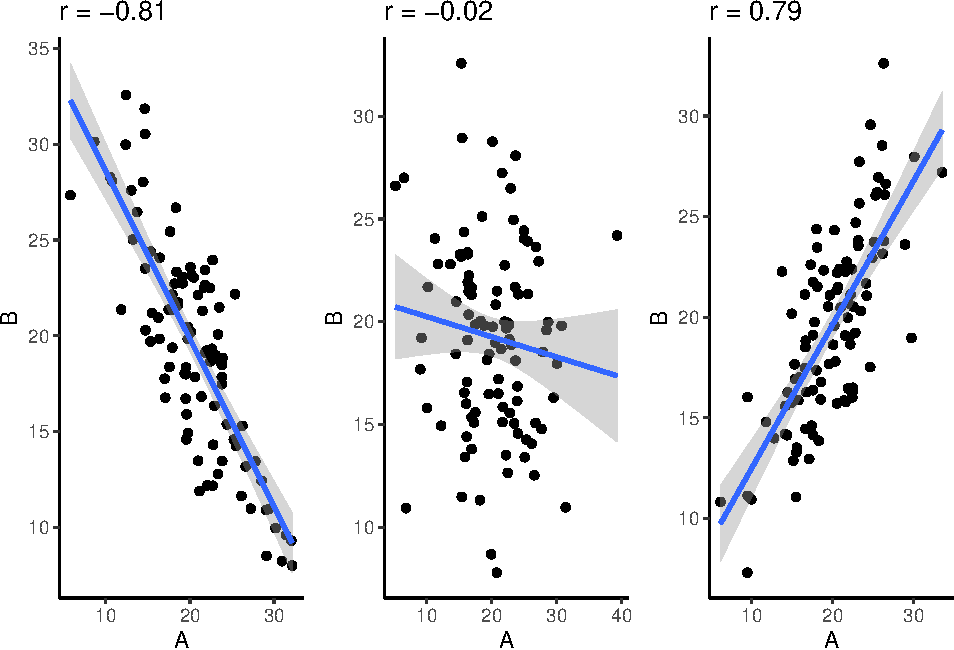
\includegraphics{CFH_R_bookdown_files/figure-latex/unnamed-chunk-206-1.pdf}

\hypertarget{hypothesen}{%
\section{Hypothesen}\label{hypothesen}}

\begin{Shaded}
\begin{Highlighting}[]
\NormalTok{data }\OtherTok{\textless{}{-}} \FunctionTok{rnorm\_multi}\NormalTok{(}\AttributeTok{n =} \DecValTok{100}\NormalTok{, }
                  \AttributeTok{mu =} \FunctionTok{c}\NormalTok{(}\DecValTok{100}\NormalTok{, }\DecValTok{8}\NormalTok{),}
                  \AttributeTok{sd =} \FunctionTok{c}\NormalTok{(}\DecValTok{25}\NormalTok{, }\DecValTok{2}\NormalTok{),}
                  \AttributeTok{r =} \FunctionTok{c}\NormalTok{(}\FloatTok{0.69}\NormalTok{), }
                  \AttributeTok{varnames =} \FunctionTok{c}\NormalTok{(}\StringTok{"Konzentration"}\NormalTok{, }\StringTok{"Schlaf"}\NormalTok{),}
                  \AttributeTok{empirical =} \ConstantTok{FALSE}\NormalTok{)}
\end{Highlighting}
\end{Shaded}

Die Korrelation prüft als Signifikanztest, ob ein Zusammenhang zwischen 2 Variablen besteht.

Da Korrelationskoeffizient von 0 bedeutet, dass kein Zusammenhang zwischen den Variablen besteht, wird im Signifikanztest i.d.R. \(r\) gegen 0 getestet (daher Nullhypothese).

Folgende Hypothesen sind denkbar:

Test auf Zusammenhang zwischen den beiden Variablen (ungerichtet):

\begin{itemize}
\tightlist
\item
  \(H_0\): \(r = 0\)
\item
  \(H_1\): \(r \neq 0\)
\end{itemize}

Test auf positiven/negativen Zusammenhang zwischen den beiden Variablen (gerichtet):

\begin{itemize}
\tightlist
\item
  \(H_0\): \(r \leq 0\)
\item
  \(H_1\): \(r > 0\)
\end{itemize}

beziehungsweise\ldots{}

\begin{itemize}
\tightlist
\item
  \(H_0\): \(r \geq 0\)
\item
  \(H_1\): \(r < 0\)
\end{itemize}

Eine typische psychologische Fragestellung für eine Zusammenhangshypothese könnte sein, ob die Anzahl der in der Nacht geschlafenen Stunden (\texttt{Schlaf}) mit der Leistung in einem Konzentrationstest zusammenhängt (\texttt{Konzentration}).

Ein entsprechender Datensatz könnte wie folgt aussehen (die ersten 6 Zeilen von \(N=100)\):

\begin{Shaded}
\begin{Highlighting}[]
\FunctionTok{head}\NormalTok{(data)}
\end{Highlighting}
\end{Shaded}

\begin{verbatim}
##   Konzentration    Schlaf
## 1     112.23087  8.450584
## 2     105.20617  8.330932
## 3     108.94331  8.488257
## 4     104.33156 10.805483
## 5      80.73751  5.933128
## 6      91.49791  7.269685
\end{verbatim}

Um einen ersten Eindruck vom Zusammenhang zu gewinnen, können wir uns die Daten in einem Streudiagramm darstellen:

\begin{Shaded}
\begin{Highlighting}[]
\FunctionTok{ggplot}\NormalTok{(}\AttributeTok{data =}\NormalTok{ data, }\FunctionTok{aes}\NormalTok{(}\AttributeTok{x =}\NormalTok{ Schlaf, }\AttributeTok{y =}\NormalTok{ Konzentration)) }\SpecialCharTok{+}
  \FunctionTok{geom\_point}\NormalTok{() }\SpecialCharTok{+}
  \FunctionTok{geom\_smooth}\NormalTok{(}\AttributeTok{method =} \StringTok{"lm"}\NormalTok{)}
\end{Highlighting}
\end{Shaded}

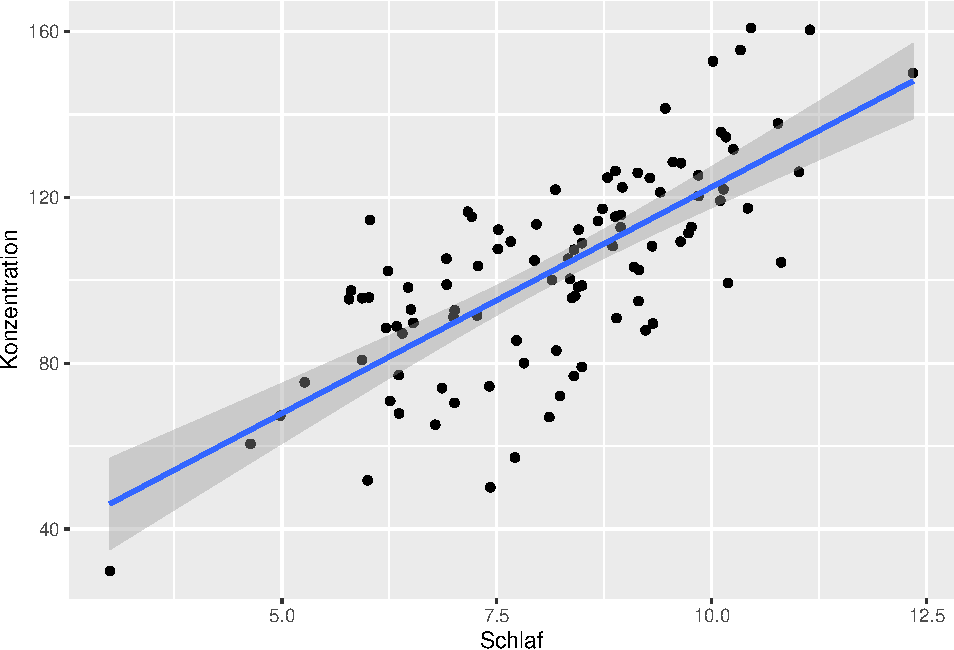
\includegraphics{CFH_R_bookdown_files/figure-latex/unnamed-chunk-209-1.pdf}

\hypertarget{berechnung-der-korrelation}{%
\section{Berechnung der Korrelation}\label{berechnung-der-korrelation}}

Der Korrelationskoeffizient lässt sich mit der R-Basisfunktion \texttt{cor()} berechnen.

Dafür schreiben wir ganz einfach die beiden zu korrelierenden Variablen nebeneinander in die Funktion:

\begin{Shaded}
\begin{Highlighting}[]
\FunctionTok{cor}\NormalTok{(data}\SpecialCharTok{$}\NormalTok{Konzentration, data}\SpecialCharTok{$}\NormalTok{Schlaf)}
\end{Highlighting}
\end{Shaded}

\begin{verbatim}
## [1] 0.732401
\end{verbatim}

Wie Sie sehen, erhalten wir einen Korrelationskoeffizienten von \(r=0.73\). Also einen positiven Zusammenhang.

\hypertarget{unterschiedliche-korrelationsmethoden}{%
\section{Unterschiedliche Korrelationsmethoden}\label{unterschiedliche-korrelationsmethoden}}

\hypertarget{pearson-korrelation}{%
\subsection{Pearson-Korrelation}\label{pearson-korrelation}}

Nutzen wir die \texttt{cor()} Funktion ohne weitere Spezifikationen, wird der sogenannte \textbf{Pearson} Korrelationskoeffizient berechnet.

Dieser stellt jedoch gewisse Voraussetzungen an die Daten:

\begin{itemize}
\tightlist
\item
  Intervallskalenniveau
\item
  keine Ausreißer
\item
  Normalverteilung der Variablen
\end{itemize}

Sollte eine (oder mehrere) der Voraussetzungen nicht erfüllt sein, berechnen wir einen der folgenden alternativen Korrelationskoeffizienten

\hypertarget{spearman-korrelation-aka-rangkorrelation}{%
\subsection{Spearman-Korrelation (aka Rangkorrelation)}\label{spearman-korrelation-aka-rangkorrelation}}

Der \textbf{Spearman} Korrelationskoeffizient funktioniert im Wesentlichen wie der Pearson Korrelationskoeffizient, jedoch wird er auf Ordinalskalenniveau berechnet.

Das macht ihn unempfindlicher gegenüber Verteilungsverletzungen und Ausreißern.

Die Berechnung des \textbf{Spearman} Korrelationskoeffizienten erfolgt nach derselben Methode, mit einer kleinen Spezifikation:

\begin{Shaded}
\begin{Highlighting}[]
\FunctionTok{cor}\NormalTok{(data}\SpecialCharTok{$}\NormalTok{Konzentration, data}\SpecialCharTok{$}\NormalTok{Schlaf, }\AttributeTok{method =} \StringTok{"spearman"}\NormalTok{)}
\end{Highlighting}
\end{Shaded}

\begin{verbatim}
## [1] 0.7183798
\end{verbatim}

In der Regel ist die Abweichung der beiden Korrelationskoeffizienten voneinander nicht allzu hoch.

\hypertarget{kendall-korrelation}{%
\subsection{Kendall-Korrelation}\label{kendall-korrelation}}

Die Rangkorrelationskoeffizienten von Spearman und Kendall sind beide Koeffizienten, die den Zusammenhang ordinalskalierter Merkmale beschreiben können.

Der Vorteil des Kendall \(τ\) liegt darin, dass seine Verteilung bei kleineren Stichprobenumfängen bessere statistische Eigenschaften bietet und er weniger empfindlich gegen Ausreißer-Rangpaare ist.

\begin{Shaded}
\begin{Highlighting}[]
\FunctionTok{cor}\NormalTok{(data}\SpecialCharTok{$}\NormalTok{Konzentration, data}\SpecialCharTok{$}\NormalTok{Schlaf, }\AttributeTok{method =} \StringTok{"kendall"}\NormalTok{)}
\end{Highlighting}
\end{Shaded}

\begin{verbatim}
## [1] 0.5292929
\end{verbatim}

\hypertarget{korrelation-als-hypothesentest}{%
\section{Korrelation als Hypothesentest}\label{korrelation-als-hypothesentest}}

Wie Sie bereits bemerkt haben werden, liefert Ihnen die \texttt{cor()} Funktion lediglich den Korrelationskoeffizienten, jedoch keine Informationen über statistische Signifikanz.

Ein Signifikanztest für den Korrelationskoeffizienten lässt sich jedoch einfach mit der Funktion \texttt{cor.test()} rechnen. Die Argumente der Funktion sind in der folgenden Tabelle zusammengefasst:

\begin{longtable}[]{@{}
  >{\raggedright\arraybackslash}p{(\columnwidth - 2\tabcolsep) * \real{0.2063}}
  >{\raggedright\arraybackslash}p{(\columnwidth - 2\tabcolsep) * \real{0.7937}}@{}}
\toprule()
\begin{minipage}[b]{\linewidth}\raggedright
Argument
\end{minipage} & \begin{minipage}[b]{\linewidth}\raggedright
Description
\end{minipage} \\
\midrule()
\endhead
\texttt{formula} & Argument in Formelformat \texttt{\textasciitilde{}\ x\ +\ y}, x und y sind die Namen der Variablen deren bivariater Zusammenhang getestet werden soll. Diese Variablen sollten in getrennten Spalten eines dataframes stehen. \\
\texttt{data} & Der data.frame, der x und y enthält \\
\texttt{alternative} & Hier kann die Richtung der Alternativhypothese angegeben werden. Wählen Sie \texttt{"two.sided"} für eine ungerichtete Hypothese, oder \texttt{"greater"} bzw. ``\texttt{less"} für eine gerichtete Hypothese. \\
\texttt{method} & Gibt die Art des zu berechnenden Korrelationskoeffizienten an. \texttt{"pearson"} (default) steht für die Produkt-Moment Korrelation, \texttt{"kendall"} und \texttt{"spearman"} stehen für die Rangkorrelatioinen nach Kendall und Spearman. \\
\texttt{subset} & Hier kann direkt ein Teildatensatz ausgewählt werden. Z.B.; \texttt{subset\ =\ sex\ ==\ "female"} \\
\bottomrule()
\end{longtable}

Wenn wir zum Beispiel testen wollten, ob ein signifikanter negativer Zusammenhang zwischen Konzentration und Schlaf besteht, könnten wir das mit folgendem Signifikanztest prüfen:

\begin{Shaded}
\begin{Highlighting}[]
\FunctionTok{cor.test}\NormalTok{(data}\SpecialCharTok{$}\NormalTok{Konzentration, data}\SpecialCharTok{$}\NormalTok{Schlaf, }\AttributeTok{method =} \StringTok{"pearson"}\NormalTok{, }\AttributeTok{alternative =} \StringTok{"less"}\NormalTok{)}
\end{Highlighting}
\end{Shaded}

\begin{verbatim}
## 
##  Pearson's product-moment correlation
## 
## data:  data$Konzentration and data$Schlaf
## t = 10.649, df = 98, p-value = 1
## alternative hypothesis: true correlation is less than 0
## 95 percent confidence interval:
##  -1.0000000  0.8008208
## sample estimates:
##      cor 
## 0.732401
\end{verbatim}

\hypertarget{tests-fuxfcr-einfache-gruppenvergleiche}{%
\chapter{Tests für einfache Gruppenvergleiche}\label{tests-fuxfcr-einfache-gruppenvergleiche}}

\hypertarget{ein-stichproben-t-test}{%
\section{Ein-Stichproben t-Test}\label{ein-stichproben-t-test}}

\begin{Shaded}
\begin{Highlighting}[]
\NormalTok{data }\OtherTok{=} \FunctionTok{read.csv}\NormalTok{(}\StringTok{"data/One sample t{-}test.csv"}\NormalTok{)}
\FunctionTok{names}\NormalTok{(data) }\OtherTok{=} \FunctionTok{c}\NormalTok{(}\StringTok{"gewicht"}\NormalTok{, }\StringTok{"groesse"}\NormalTok{)}
\end{Highlighting}
\end{Shaded}

\hypertarget{hypothesen-1}{%
\subsection{Hypothesen}\label{hypothesen-1}}

Mit einem Ein-Stichproben t-Test vergleichen wir den Mittelwert einer Gruppe mit einem hypothetischen Mittelwert.

Der Test prüft also anhand des Mittelwerts einer Stichprobe, ob der Erwartungswert in der entsprechenden Population gleich einem vorgegebenen Wert ist (dem unter \(H_{0}\) erwarteten \(μ_{0}\)).

Es sind folgende Hypothesen denkbar:

Test auf Unterschiedlichkeit von dem Referenzwert (ungerichtet):

\begin{itemize}
\tightlist
\item
  \(H_0\): \(μ=μ_{0}\)
\item
  \(H_1\): \(μ\neqμ_0\)
\end{itemize}

Test, ob Mittelwert größer/kleiner als Referenzwert ist (gerichtet):

\begin{itemize}
\tightlist
\item
  \(H_0\): \(μ≤μ_{0}\); \(H_1\): \(μ>μ_{0}\)
\item
  \(H_0\): \(μ≥μ_{0}\); \(H_1\): \(μ<μ_{0}\)
\end{itemize}

Zum Beispiel könnten wir eine Stichprobe von Menschen aus Deutschland erhoben haben und uns dafür interessieren, ob diese signifikant größer, bzw. kleiner als der Durchschnitt in Deutschland sind.

Die ersten Zeilen des Stichprobendatensatzes könnten so aussehen:

\begin{verbatim}
##   gewicht groesse
## 1      77     182
## 2      68     177
## 3      76     170
## 4      76     167
## 5      69     186
## 6      71     178
\end{verbatim}

Zunächst brauchen wir einen hypothetischen Vergleichswert. Sucht man die geschlechterübergreifende Durchschnittsgröße in Deutschland im Internet findet man einen Wert von ca. 173 cm.

\hypertarget{deskriptive-einordnung}{%
\subsection{Deskriptive Einordnung}\label{deskriptive-einordnung}}

Die Berechnung unseres Mittelwerts ist einfache Deskriptivstatistik:

\begin{Shaded}
\begin{Highlighting}[]
\FunctionTok{mean}\NormalTok{(data}\SpecialCharTok{$}\NormalTok{groesse)}
\end{Highlighting}
\end{Shaded}

\begin{verbatim}
## [1] 177.6087
\end{verbatim}

Der Sachverhalt lässt sich auch graphisch darstellen:

\begin{Shaded}
\begin{Highlighting}[]
\FunctionTok{ggplot}\NormalTok{(}\AttributeTok{data =}\NormalTok{ data, }\FunctionTok{aes}\NormalTok{(}\AttributeTok{x =}\NormalTok{ groesse)) }\SpecialCharTok{+}
  \FunctionTok{geom\_histogram}\NormalTok{(}\AttributeTok{bins =} \DecValTok{40}\NormalTok{, }\AttributeTok{fill =} \StringTok{"black"}\NormalTok{) }\SpecialCharTok{+}
  \FunctionTok{labs}\NormalTok{(}\AttributeTok{x =} \StringTok{"Größe"}\NormalTok{, }\AttributeTok{y =} \StringTok{"N"}\NormalTok{) }\SpecialCharTok{+}
  \FunctionTok{geom\_vline}\NormalTok{(}\AttributeTok{xintercept =} \DecValTok{173}\NormalTok{, }\AttributeTok{linetype =} \StringTok{"dashed"}\NormalTok{, }\AttributeTok{colour =} \StringTok{"red"}\NormalTok{) }\SpecialCharTok{+}
  \FunctionTok{geom\_vline}\NormalTok{(}\AttributeTok{xintercept =} \FunctionTok{mean}\NormalTok{(data}\SpecialCharTok{$}\NormalTok{groesse), }\AttributeTok{linetype =} \StringTok{"dashed"}\NormalTok{, }\AttributeTok{colour =} \StringTok{"green"}\NormalTok{) }\SpecialCharTok{+}
  \FunctionTok{theme\_classic}\NormalTok{() }
\end{Highlighting}
\end{Shaded}

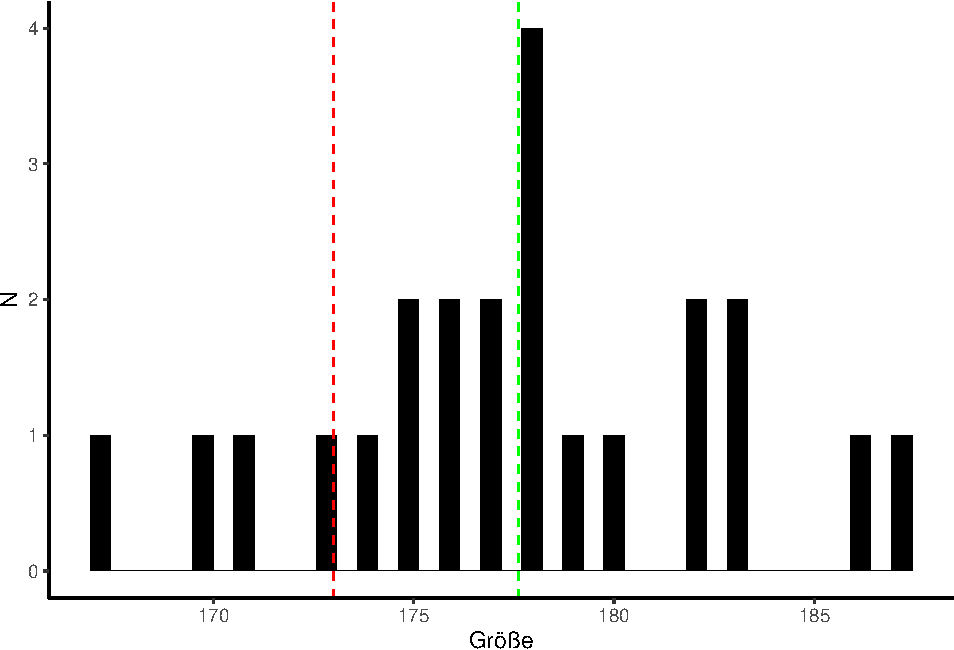
\includegraphics{CFH_R_bookdown_files/figure-latex/unnamed-chunk-218-1.pdf}

Die grüne Linie im Zentrum des Histogramms stellt unseren Stichprobenmittelwert dar. Die rote Linie ist der angenommene Mittelwert in der Population von 173 cm.

\hypertarget{test-durchfuxfchren}{%
\subsection{Test durchführen}\label{test-durchfuxfchren}}

Zur Durchführung des Tests nutzen wir die in der Grundform von R vorinstallierte \texttt{t.test()} Funktion.

\begin{Shaded}
\begin{Highlighting}[]
\FunctionTok{t.test}\NormalTok{(data}\SpecialCharTok{$}\NormalTok{groesse, }\AttributeTok{mu =} \DecValTok{173}\NormalTok{, }\AttributeTok{alternative =} \StringTok{"two.sided"}\NormalTok{, }\AttributeTok{conf.level =} \FloatTok{0.95}\NormalTok{)}
\end{Highlighting}
\end{Shaded}

\begin{verbatim}
## 
##  One Sample t-test
## 
## data:  data$groesse
## t = 4.4969, df = 22, p-value = 0.0001792
## alternative hypothesis: true mean is not equal to 173
## 95 percent confidence interval:
##  175.4833 179.7341
## sample estimates:
## mean of x 
##  177.6087
\end{verbatim}

Wir wählen die Variable \texttt{groesse} innerhalb unseres Datensatzes mit dem \texttt{\$} Zeichen an. Über das \texttt{mu} Argument geben wir den hypothetischen Vergleichswert an. Unter \texttt{alternative} können wir auswählen, ob der Test gerichtet oder ungerichtet (aka ein- oder zweiseitig) durchgeführt werden soll. Je nach Hypothese wählen wir \texttt{"two.sided"} für einen ungerichteten Test und entweder \texttt{"less"} oder \texttt{"greater"} für einen gerichteten Test. Das \texttt{conf.level} entsprich unserem Signifikanzniveau.

\hypertarget{ergebnis-interpretieren}{%
\subsection{Ergebnis interpretieren}\label{ergebnis-interpretieren}}

Das Ergebnis des Tests lässt sich am P-Wert ablesen (p=0.0001792). Ist der P-wert kleiner als das gewählte Signifikanzniveau (i.d.R \(\alpha=.05\)) unterscheidet sich unser Stichprobenmittelwert (177.61 cm) signifikant von der Durchschnittsgröße in Deutschland (173 cm). Wir verwerfen also die Nullhypothese (H0) zugunsten unserer Alternativhypothese (H1).

\hypertarget{ergebnis-berichten}{%
\subsection{Ergebnis berichten}\label{ergebnis-berichten}}

Die relevanten Parameter zum Berichten eines Ein-Stichproben t-Tests sind

\begin{itemize}
\tightlist
\item
  M (Mittelwert)
\item
  Grenzen des Konfidenzintervalls des Mittelwerts
\item
  t-Wert (Teststatistik)
\item
  df (Freiheitsgerade)
\item
  P-Wert
\end{itemize}

Beim Berichten im Fließtext schreibt man:

Die Größe in der Stichpobe unterschied sich signifikant von der Durchschnittsgröße in Deutschland (173 cm), M = 177.61, 95\% CI (175.48, 179.73), t (22) = 4.5; p \textless{} .001.

Diese Werte lassen sich wie folgt aus dem t-Test Objekt extrahieren:

t-Wert (Teststatistik):

\begin{Shaded}
\begin{Highlighting}[]
\FunctionTok{t.test}\NormalTok{(data}\SpecialCharTok{$}\NormalTok{groesse, }\AttributeTok{mu =} \DecValTok{173}\NormalTok{, }\AttributeTok{alternative =} \StringTok{"two.sided"}\NormalTok{, }\AttributeTok{conf.level =} \FloatTok{0.95}\NormalTok{)}\SpecialCharTok{$}\NormalTok{statistic}
\end{Highlighting}
\end{Shaded}

\begin{verbatim}
##        t 
## 4.496872
\end{verbatim}

df (Freiheitsgerade):

\begin{Shaded}
\begin{Highlighting}[]
\FunctionTok{t.test}\NormalTok{(data}\SpecialCharTok{$}\NormalTok{groesse, }\AttributeTok{mu =} \DecValTok{173}\NormalTok{, }\AttributeTok{alternative =} \StringTok{"two.sided"}\NormalTok{, }\AttributeTok{conf.level =} \FloatTok{0.95}\NormalTok{)}\SpecialCharTok{$}\NormalTok{parameter}
\end{Highlighting}
\end{Shaded}

\begin{verbatim}
## df 
## 22
\end{verbatim}

P-Wert:

\begin{Shaded}
\begin{Highlighting}[]
\FunctionTok{t.test}\NormalTok{(data}\SpecialCharTok{$}\NormalTok{groesse, }\AttributeTok{mu =} \DecValTok{173}\NormalTok{, }\AttributeTok{alternative =} \StringTok{"two.sided"}\NormalTok{, }\AttributeTok{conf.level =} \FloatTok{0.95}\NormalTok{)}\SpecialCharTok{$}\NormalTok{p.value}
\end{Highlighting}
\end{Shaded}

\begin{verbatim}
## [1] 0.0001792355
\end{verbatim}

Grenzen des Konfidenzintervalls (unten \& oben):

\begin{Shaded}
\begin{Highlighting}[]
\FunctionTok{t.test}\NormalTok{(data}\SpecialCharTok{$}\NormalTok{groesse, }\AttributeTok{mu =} \DecValTok{173}\NormalTok{, }\AttributeTok{alternative =} \StringTok{"two.sided"}\NormalTok{, }\AttributeTok{conf.level =} \FloatTok{0.95}\NormalTok{)}\SpecialCharTok{$}\NormalTok{conf.int[}\DecValTok{1}\NormalTok{]}
\end{Highlighting}
\end{Shaded}

\begin{verbatim}
## [1] 175.4833
\end{verbatim}

\begin{Shaded}
\begin{Highlighting}[]
\FunctionTok{t.test}\NormalTok{(data}\SpecialCharTok{$}\NormalTok{groesse, }\AttributeTok{mu =} \DecValTok{173}\NormalTok{, }\AttributeTok{alternative =} \StringTok{"two.sided"}\NormalTok{, }\AttributeTok{conf.level =} \FloatTok{0.95}\NormalTok{)}\SpecialCharTok{$}\NormalTok{conf.int[}\DecValTok{2}\NormalTok{]}
\end{Highlighting}
\end{Shaded}

\begin{verbatim}
## [1] 179.7341
\end{verbatim}

\hypertarget{effektstuxe4rke}{%
\subsection{Effektstärke}\label{effektstuxe4rke}}

\hypertarget{cohens-d}{%
\subsubsection{Cohen's d}\label{cohens-d}}

Die am häufigsten verwendete Effektstärke für den Ein-Stichproben t-Test ist Cohen's d \citet{cohen1988statistical}.
Cohen's d lässt sich mit dem Paket \texttt{effsize} berechnen. Dieses verwendet praktischerweise die gleiche Schreibweise, wie der t-Test:

\begin{Shaded}
\begin{Highlighting}[]
\NormalTok{effsize}\SpecialCharTok{::}\FunctionTok{cohen.d}\NormalTok{(data}\SpecialCharTok{$}\NormalTok{groesse, }\AttributeTok{f =} \ConstantTok{NA}\NormalTok{, }\AttributeTok{mu =} \DecValTok{173}\NormalTok{)}
\end{Highlighting}
\end{Shaded}

\begin{verbatim}
## 
## Cohen's d (single sample)
## 
## d estimate: 0.9376626 (large)
## Reference mu: 173
## 95 percent confidence interval:
##      lower      upper 
## 0.02651145 1.84881385
\end{verbatim}

Auch die Einzelparameter von Cohen's d lassen sich extrahieren:

Cohen's d:

\begin{Shaded}
\begin{Highlighting}[]
\NormalTok{effsize}\SpecialCharTok{::}\FunctionTok{cohen.d}\NormalTok{(}\AttributeTok{d =}\NormalTok{ data}\SpecialCharTok{$}\NormalTok{groesse, }\AttributeTok{f =} \ConstantTok{NA}\NormalTok{, }\AttributeTok{mu =} \DecValTok{173}\NormalTok{)}\SpecialCharTok{$}\NormalTok{estimate}
\end{Highlighting}
\end{Shaded}

\begin{verbatim}
## [1] 0.9376626
\end{verbatim}

Grenzen des Konfidenzintervalls (unten \& oben):

\begin{Shaded}
\begin{Highlighting}[]
\NormalTok{effsize}\SpecialCharTok{::}\FunctionTok{cohen.d}\NormalTok{(}\AttributeTok{d =}\NormalTok{ data}\SpecialCharTok{$}\NormalTok{groesse, }\AttributeTok{f =} \ConstantTok{NA}\NormalTok{, }\AttributeTok{mu =} \DecValTok{173}\NormalTok{)}\SpecialCharTok{$}\NormalTok{conf.int[}\DecValTok{1}\NormalTok{]}
\end{Highlighting}
\end{Shaded}

\begin{verbatim}
##      lower 
## 0.02651145
\end{verbatim}

\begin{Shaded}
\begin{Highlighting}[]
\NormalTok{effsize}\SpecialCharTok{::}\FunctionTok{cohen.d}\NormalTok{(}\AttributeTok{d =}\NormalTok{ data}\SpecialCharTok{$}\NormalTok{groesse, }\AttributeTok{f =} \ConstantTok{NA}\NormalTok{, }\AttributeTok{mu =} \DecValTok{173}\NormalTok{)}\SpecialCharTok{$}\NormalTok{conf.int[}\DecValTok{2}\NormalTok{]}
\end{Highlighting}
\end{Shaded}

\begin{verbatim}
##    upper 
## 1.848814
\end{verbatim}

Die Interpretation von Cohens'd lautet wie folgt \citet{cohen1992quantitative}:

\begin{table}[tbp]

\begin{center}
\begin{threeparttable}

\caption{\label{tab:unnamed-chunk-227}Interpretation von Cohen's d.}

\begin{tabular}{ll}
\toprule
d & \multicolumn{1}{c}{Interpretation}\\
\midrule
|>0.2| & kleiner Effekt\\
|>0.5| & mittlerer Effekt\\
|>0.8| & großer Effekt\\
\bottomrule
\end{tabular}

\end{threeparttable}
\end{center}

\end{table}

\hypertarget{darstellung-in-tabellenform}{%
\subsection{Darstellung in Tabellenform}\label{darstellung-in-tabellenform}}

Zur sauberen Darstellung des Ergebnisses in einer bereits nach APA formatierten Tabelle, lassen sich die Funktionen \texttt{apa\_print} und \texttt{apa\_table} aus dem Paket \texttt{papaja} verwenden.

\begin{Shaded}
\begin{Highlighting}[]
\FunctionTok{library}\NormalTok{(papaja)}
\NormalTok{apa\_test }\OtherTok{\textless{}{-}} \FunctionTok{apa\_print}\NormalTok{(}
  \FunctionTok{t.test}\NormalTok{(data}\SpecialCharTok{$}\NormalTok{groesse, }\AttributeTok{mu =} \DecValTok{173}\NormalTok{, }\AttributeTok{alternative =} \StringTok{"two.sided"}\NormalTok{, }\AttributeTok{conf.level =} \FloatTok{0.95}\NormalTok{)}
\NormalTok{)}
\FunctionTok{apa\_table}\NormalTok{(}
\NormalTok{  apa\_test}\SpecialCharTok{$}\NormalTok{table, }\AttributeTok{caption =} \StringTok{"Tabelle für den Ein{-}Stichproben t{-}Test."}
\NormalTok{)}
\end{Highlighting}
\end{Shaded}

\begin{table}[tbp]

\begin{center}
\begin{threeparttable}

\caption{\label{tab:unnamed-chunk-228}Tabelle für den Ein-Stichproben t-Test.}

\begin{tabular}{lllll}
\toprule
$M$ & \multicolumn{1}{c}{95\% CI} & \multicolumn{1}{c}{$t$} & \multicolumn{1}{c}{$\mathit{df}$} & \multicolumn{1}{c}{$p$}\\
\midrule
177.61 & {}[175.48, 179.73] & 4.50 & 22 & < .001\\
\bottomrule
\end{tabular}

\end{threeparttable}
\end{center}

\end{table}

\hypertarget{t-test-bei-unabhuxe4ngigen-stichproben}{%
\section{t-Test bei unabhängigen Stichproben}\label{t-test-bei-unabhuxe4ngigen-stichproben}}

\hypertarget{hypothesen-2}{%
\subsection{Hypothesen}\label{hypothesen-2}}

Mit einem unabhängigen t-Test vergleichen wir die Mittelwerte von 2 unabhängigen Gruppen. Im Datensatz müssen zwei Variablen vorhanden sein, eine numerische Variable (AV), für die Mittelwerte berechnet werden können und eine dichotome Gruppenvariable (UV).

Es sind folgende Hypothesen denkbar:

Test auf Unterschiedlichkeit der beiden Gruppenmittelwerte (ungerichtet):

\begin{itemize}
\tightlist
\item
  \(H_0\): \(μ_1=μ_2\) bzw. \(μ_1−μ_2=0\) und \(σ_1=σ_2=σ\)
\item
  \(H_1\): \(μ_1\neqμ_2\) bzw. \(μ_1−μ_2\neq0\) und \(σ_1=σ_2=σ\)
\end{itemize}

Test, ob Mittelwert der einen Gruppe größer/kleiner als Mittelwert der anderen Gruppe ist (gerichtet):

\begin{itemize}
\tightlist
\item
  \(H_0\): \(μ_1\leqμ_2\) bzw. \(μ_1−μ_2\leq0\) und \(σ_1=σ_2=σ\)
\item
  \(H_1\): \(μ_1>μ_2\) bzw. \(μ_1−μ_2>0\) und \(σ_1=σ_2=σ\)
\end{itemize}

Zum Beispiel könnten wir eine Stichprobe bestehend aus Männern und Frauen erhoben haben, die eine Diät durchgeführt haben. Eine Fragestellung könnte sein, ob Männer und Frauen (Geschlecht = dichotome UV) unterschiedlich viel abgenommen haben (Gewichtsverlust = numerische AV).

Die ersten Zeilen des Stichprobendatensatzes könnten so aussehen:

\begin{verbatim}
##   Gender Weight.loss
## 1  Males         0.0
## 2  Males         0.0
## 3  Males         3.8
## 4  Males         6.0
## 5  Males         0.7
## 6  Males         2.9
\end{verbatim}

\hypertarget{deskriptive-einordnung-1}{%
\subsection{Deskriptive Einordnung}\label{deskriptive-einordnung-1}}

Zunächst können wir uns die Deskriptivstatistiken innerhalb der beiden Gruppen einmal anschauen:

\begin{Shaded}
\begin{Highlighting}[]
\NormalTok{psych}\SpecialCharTok{::}\FunctionTok{describeBy}\NormalTok{(Weight.loss }\SpecialCharTok{\textasciitilde{}}\NormalTok{ Gender, }\AttributeTok{data =}\NormalTok{ data)}
\end{Highlighting}
\end{Shaded}

\begin{verbatim}
## 
##  Descriptive statistics by group 
## Gender: Females
##             vars  n mean   sd median trimmed  mad min  max range skew kurtosis
## Weight.loss    1 42 6.93 2.24      7     6.9 1.93 1.6 12.2  10.6 0.12     0.38
##               se
## Weight.loss 0.35
## ------------------------------------------------------------ 
## Gender: Males
##             vars  n mean   sd median trimmed  mad  min max range skew kurtosis
## Weight.loss    1 45 3.72 2.59    3.4    3.75 2.82 -2.1 8.5  10.6 0.01    -0.92
##               se
## Weight.loss 0.39
\end{verbatim}

Rein deskriptiv lässt sich bereits feststellen, dass Männer mit 3.72kg etwas weniger abgenommen zu haben scheinen, als Frauen mit 3.72kg.

Ob sich dieser numerische Unterschied auch als signifikant erweist, prüfen wir mit dem t-Test.

\hypertarget{test-durchfuxfchren-1}{%
\subsection{Test durchführen}\label{test-durchfuxfchren-1}}

Zur Durchführung des Tests nutzen wir die in der Grundform von R vorinstallierte \texttt{t.test()} Funktion.

Die Schreibweise in Formelformat nimmt die Form \texttt{AV\ \textasciitilde{}\ UV} an, wobei \texttt{\textasciitilde{}} soviel heißt wie ``wird vorhergesagt durch''.

\begin{Shaded}
\begin{Highlighting}[]
\FunctionTok{t.test}\NormalTok{(Weight.loss }\SpecialCharTok{\textasciitilde{}}\NormalTok{ Gender, }\AttributeTok{data =}\NormalTok{ data)}
\end{Highlighting}
\end{Shaded}

\begin{verbatim}
## 
##  Welch Two Sample t-test
## 
## data:  Weight.loss by Gender
## t = 6.191, df = 84.544, p-value = 0.00000002069
## alternative hypothesis: true difference in means is not equal to 0
## 95 percent confidence interval:
##  2.178046 4.239097
## sample estimates:
## mean in group Females   mean in group Males 
##              6.928571              3.720000
\end{verbatim}

Alternative Schreibweise:

\begin{Shaded}
\begin{Highlighting}[]
\FunctionTok{t.test}\NormalTok{(data}\SpecialCharTok{$}\NormalTok{Weight.loss[data}\SpecialCharTok{$}\NormalTok{Gender }\SpecialCharTok{==} \StringTok{"Males"}\NormalTok{], data}\SpecialCharTok{$}\NormalTok{Weight.loss[data}\SpecialCharTok{$}\NormalTok{Gender }\SpecialCharTok{==} \StringTok{"Females"}\NormalTok{])}
\end{Highlighting}
\end{Shaded}

\begin{verbatim}
## 
##  Welch Two Sample t-test
## 
## data:  data$Weight.loss[data$Gender == "Males"] and data$Weight.loss[data$Gender == "Females"]
## t = -6.191, df = 84.544, p-value = 0.00000002069
## alternative hypothesis: true difference in means is not equal to 0
## 95 percent confidence interval:
##  -4.239097 -2.178046
## sample estimates:
## mean of x mean of y 
##  3.720000  6.928571
\end{verbatim}

Für einen gerichteten Test (z.B. Frauen nehmen mehr ab als Männer)

\begin{Shaded}
\begin{Highlighting}[]
\FunctionTok{t.test}\NormalTok{(Weight.loss }\SpecialCharTok{\textasciitilde{}}\NormalTok{ Gender, }\AttributeTok{data =}\NormalTok{ data, }\AttributeTok{alternative =} \StringTok{"greater"}\NormalTok{)}
\end{Highlighting}
\end{Shaded}

\begin{verbatim}
## 
##  Welch Two Sample t-test
## 
## data:  Weight.loss by Gender
## t = 6.191, df = 84.544, p-value = 0.00000001035
## alternative hypothesis: true difference in means is greater than 0
## 95 percent confidence interval:
##  2.34666     Inf
## sample estimates:
## mean in group Females   mean in group Males 
##              6.928571              3.720000
\end{verbatim}

\hypertarget{relevante-parameter-extrahieren}{%
\subsection{Relevante Parameter extrahieren}\label{relevante-parameter-extrahieren}}

Die relevanten Parameter zum Berichten eines unabhängigen t-Tests sind:

\begin{itemize}
\tightlist
\item
  \(\Delta\)M (Differenz vom Mittelwert zum Referenzwert)
\item
  Grenzen des Konfidenzintervalls der Mittelwertsdifferenz
\item
  t-Wert (Teststatistik)
\item
  df (Freiheitsgerade)
\item
  P-Wert
\end{itemize}

Diese Werte lassen sich wie folgt aus dem t-Test Objekt extrahieren:

t-Wert (Teststatistik):

\begin{Shaded}
\begin{Highlighting}[]
\FunctionTok{t.test}\NormalTok{(Weight.loss }\SpecialCharTok{\textasciitilde{}}\NormalTok{ Gender, }\AttributeTok{data =}\NormalTok{ data)}\SpecialCharTok{$}\NormalTok{statistic}
\end{Highlighting}
\end{Shaded}

\begin{verbatim}
##        t 
## 6.191013
\end{verbatim}

df (Freiheitsgerade):

\begin{Shaded}
\begin{Highlighting}[]
\FunctionTok{t.test}\NormalTok{(Weight.loss }\SpecialCharTok{\textasciitilde{}}\NormalTok{ Gender, }\AttributeTok{data =}\NormalTok{ data)}\SpecialCharTok{$}\NormalTok{parameter}
\end{Highlighting}
\end{Shaded}

\begin{verbatim}
##     df 
## 84.544
\end{verbatim}

P-Wert:

\begin{Shaded}
\begin{Highlighting}[]
\FunctionTok{t.test}\NormalTok{(Weight.loss }\SpecialCharTok{\textasciitilde{}}\NormalTok{ Gender, }\AttributeTok{data =}\NormalTok{ data)}\SpecialCharTok{$}\NormalTok{p.value}
\end{Highlighting}
\end{Shaded}

\begin{verbatim}
## [1] 0.00000002069288
\end{verbatim}

Grenzen des Konfidenzintervalls (unten \& oben):

\begin{Shaded}
\begin{Highlighting}[]
\FunctionTok{t.test}\NormalTok{(Weight.loss }\SpecialCharTok{\textasciitilde{}}\NormalTok{ Gender, }\AttributeTok{data =}\NormalTok{ data)}\SpecialCharTok{$}\NormalTok{conf.int[}\DecValTok{1}\NormalTok{]}
\end{Highlighting}
\end{Shaded}

\begin{verbatim}
## [1] 2.178046
\end{verbatim}

\begin{Shaded}
\begin{Highlighting}[]
\FunctionTok{t.test}\NormalTok{(Weight.loss }\SpecialCharTok{\textasciitilde{}}\NormalTok{ Gender, }\AttributeTok{data =}\NormalTok{ data)}\SpecialCharTok{$}\NormalTok{conf.int[}\DecValTok{2}\NormalTok{]}
\end{Highlighting}
\end{Shaded}

\begin{verbatim}
## [1] 4.239097
\end{verbatim}

\hypertarget{voraussetzungspruxfcfung-und-alternativen}{%
\subsection{Voraussetzungsprüfung und Alternativen}\label{voraussetzungspruxfcfung-und-alternativen}}

Folgende Vorraussetzungen gelten für den unabhängigen t-Test:
* unabhängige Messungen
* Intervallskala
* Normalverteilung in beiden Gruppen
* Homogenität der Varianzen

Sollten die Vorraussetzungen Intervallskalekniveau und Normalverteilung verletzt sein, muss ein robuster Test gerechnet werden (s.u. U-Test).

Die Varianzhomogenität wird mittels Levene's Test (F-Test) geprüft \citet{levene1960robust}. Eine Funktion dafür ist im Patek \texttt{car} enthalten.

\begin{Shaded}
\begin{Highlighting}[]
\NormalTok{car}\SpecialCharTok{::}\FunctionTok{leveneTest}\NormalTok{(Weight.loss }\SpecialCharTok{\textasciitilde{}}\NormalTok{ Gender, }\AttributeTok{data =}\NormalTok{ data)}
\end{Highlighting}
\end{Shaded}

\begin{verbatim}
## Levene's Test for Homogeneity of Variance (center = median)
##       Df F value Pr(>F)
## group  1  2.0175 0.1591
##       85
\end{verbatim}

Ein signifikanter Levene's Test bedeutet, dass sich die Varianzen innerhalb der Gruppen signifikant unterscheiden. Sie sind also nicht ``homogen''.

Zum Berichten eines Levene's Test gibt es nicht viel zu tun. Lediglich die Freiheitsgrade, der F-Wert und die Signifikanz sind zu berichten. Die übliche Form hierfür ist die folgende: F(1,49) = 16,908, p = 0,0001493

Liegt keine Varianzhomogenität vor, berechnet man stattdessen einen \textbf{Welch-Test}.

Um einen \textbf{Welch-Test} zu berechnen, ändern wir nur leicht die Funktion:

\begin{Shaded}
\begin{Highlighting}[]
\FunctionTok{t.test}\NormalTok{(Weight.loss }\SpecialCharTok{\textasciitilde{}}\NormalTok{ Gender, }\AttributeTok{data =}\NormalTok{ data, }\AttributeTok{var.equal =} \ConstantTok{FALSE}\NormalTok{)}
\end{Highlighting}
\end{Shaded}

\begin{verbatim}
## 
##  Welch Two Sample t-test
## 
## data:  Weight.loss by Gender
## t = 6.191, df = 84.544, p-value = 0.00000002069
## alternative hypothesis: true difference in means is not equal to 0
## 95 percent confidence interval:
##  2.178046 4.239097
## sample estimates:
## mean in group Females   mean in group Males 
##              6.928571              3.720000
\end{verbatim}

\hypertarget{effektstuxe4rke-1}{%
\subsection{Effektstärke}\label{effektstuxe4rke-1}}

\hypertarget{cohens-d-1}{%
\subsubsection{Cohen's d}\label{cohens-d-1}}

Die am häufigsten verwendete Effektstärke für den Vergleich zweier unabhängiger Gruppen ist Cohen's d \citet{cohen1988statistical}.
Cohen's d lässt sich mit dem Paket \texttt{effsize} berechnen. Dieses verwendet praktischerweise die gleiche Schreibweise, wie der t-Test:

\begin{Shaded}
\begin{Highlighting}[]
\NormalTok{effsize}\SpecialCharTok{::}\FunctionTok{cohen.d}\NormalTok{(Weight.loss }\SpecialCharTok{\textasciitilde{}}\NormalTok{ Gender, }\AttributeTok{data =}\NormalTok{ data)}
\end{Highlighting}
\end{Shaded}

\begin{verbatim}
## 
## Cohen's d
## 
## d estimate: 1.321689 (large)
## 95 percent confidence interval:
##     lower     upper 
## 0.8508801 1.7924981
\end{verbatim}

Auch die Einzelparameter von Cohen's d lassen sich extrahieren:

Cohen's d:

\begin{Shaded}
\begin{Highlighting}[]
\NormalTok{effsize}\SpecialCharTok{::}\FunctionTok{cohen.d}\NormalTok{(Weight.loss }\SpecialCharTok{\textasciitilde{}}\NormalTok{ Gender, }\AttributeTok{data =}\NormalTok{ data)}\SpecialCharTok{$}\NormalTok{estimate}
\end{Highlighting}
\end{Shaded}

\begin{verbatim}
## [1] 1.321689
\end{verbatim}

Grenzen des Konfidenzintervalls (unten \& oben):

\begin{Shaded}
\begin{Highlighting}[]
\NormalTok{effsize}\SpecialCharTok{::}\FunctionTok{cohen.d}\NormalTok{(Weight.loss }\SpecialCharTok{\textasciitilde{}}\NormalTok{ Gender, }\AttributeTok{data =}\NormalTok{ data)}\SpecialCharTok{$}\NormalTok{conf.int[}\DecValTok{1}\NormalTok{]}
\end{Highlighting}
\end{Shaded}

\begin{verbatim}
##     lower 
## 0.8508801
\end{verbatim}

\begin{Shaded}
\begin{Highlighting}[]
\NormalTok{effsize}\SpecialCharTok{::}\FunctionTok{cohen.d}\NormalTok{(Weight.loss }\SpecialCharTok{\textasciitilde{}}\NormalTok{ Gender, }\AttributeTok{data =}\NormalTok{ data)}\SpecialCharTok{$}\NormalTok{conf.int[}\DecValTok{2}\NormalTok{]}
\end{Highlighting}
\end{Shaded}

\begin{verbatim}
##    upper 
## 1.792498
\end{verbatim}

Die Interpretation von Cohens'd lautet wie folgt \citet{cohen1992quantitative}:

\begin{table}[tbp]

\begin{center}
\begin{threeparttable}

\caption{\label{tab:unnamed-chunk-244}Interpretation von Cohen's d.}

\begin{tabular}{ll}
\toprule
d & \multicolumn{1}{c}{Interpretation}\\
\midrule
|>0.2| & kleiner Effekt\\
|>0.5| & mittlerer Effekt\\
|>0.8| & großer Effekt\\
\bottomrule
\end{tabular}

\end{threeparttable}
\end{center}

\end{table}

\hypertarget{hedges-g}{%
\subsubsection{Hedges' g}\label{hedges-g}}

Eine gelegentlich verwendete Alternative zu Cohen's d ist das Hedges' g. Hedges' g wird weitgehend analog zu Cohen's d verwendet, korrigiert dabei jedoch statistisch für besonders kleine Gruppengößen (N\textless20) \citet{hedges2014statistical}

Es lässt sich mit derselben Funktion berechnen:

\begin{Shaded}
\begin{Highlighting}[]
\NormalTok{effsize}\SpecialCharTok{::}\FunctionTok{cohen.d}\NormalTok{(Weight.loss }\SpecialCharTok{\textasciitilde{}}\NormalTok{ Gender, }\AttributeTok{data =}\NormalTok{ data, }\AttributeTok{hedges.correction =} \ConstantTok{TRUE}\NormalTok{)}
\end{Highlighting}
\end{Shaded}

\begin{verbatim}
## 
## Hedges's g
## 
## g estimate: 1.309993 (large)
## 95 percent confidence interval:
##     lower     upper 
## 0.8440869 1.7758986
\end{verbatim}

Die Interpretation von Hedges' g ist identisch wie die von von Cohens'd:

\begin{table}[tbp]

\begin{center}
\begin{threeparttable}

\caption{\label{tab:unnamed-chunk-246}Interpretation von Hedges' g.}

\begin{tabular}{ll}
\toprule
g & \multicolumn{1}{c}{Interpretation}\\
\midrule
|>0.2| & kleiner Effekt\\
|>0.5| & mittlerer Effekt\\
|>0.8| & großer Effekt\\
\bottomrule
\end{tabular}

\end{threeparttable}
\end{center}

\end{table}

\hypertarget{darstellung-in-tabellenform-1}{%
\subsection{Darstellung in Tabellenform}\label{darstellung-in-tabellenform-1}}

Zur sauberen Darstellung des Ergebnisses in einer bereits nach APA formatierten Tabelle, lassen sich die Funktionen \texttt{apa\_print} und \texttt{apa\_table} aus dem Paket \texttt{papaja} verwenden.

\begin{Shaded}
\begin{Highlighting}[]
\FunctionTok{library}\NormalTok{(papaja)}
\NormalTok{apa\_test }\OtherTok{\textless{}{-}} \FunctionTok{apa\_print}\NormalTok{(}
 \FunctionTok{t.test}\NormalTok{(Weight.loss }\SpecialCharTok{\textasciitilde{}}\NormalTok{ Gender, }\AttributeTok{data =}\NormalTok{ data)}
\NormalTok{)}
\FunctionTok{apa\_table}\NormalTok{(}
\NormalTok{  apa\_test}\SpecialCharTok{$}\NormalTok{table, }\AttributeTok{caption =} \StringTok{"Tabelle für den unabhängigen t{-}Test."}
\NormalTok{)}
\end{Highlighting}
\end{Shaded}

\begin{table}[tbp]

\begin{center}
\begin{threeparttable}

\caption{\label{tab:unnamed-chunk-247}Tabelle für den unabhängigen t-Test.}

\begin{tabular}{lllll}
\toprule
$\Delta M$ & \multicolumn{1}{c}{95\% CI} & \multicolumn{1}{c}{$t$} & \multicolumn{1}{c}{$\mathit{df}$} & \multicolumn{1}{c}{$p$}\\
\midrule
3.21 & {}[2.18, 4.24] & 6.19 & 84.54 & < .001\\
\bottomrule
\end{tabular}

\end{threeparttable}
\end{center}

\end{table}

\hypertarget{t-test-bei-abhuxe4ngigen-stichproben}{%
\section{t-Test bei abhängigen Stichproben}\label{t-test-bei-abhuxe4ngigen-stichproben}}

\hypertarget{hypothesen-3}{%
\subsection{Hypothesen}\label{hypothesen-3}}

Mit einem abhängigen t-Test vergleichen wir die Mittelwerte zweier abhängiger Messungen. Ein klassisches Beispiel dafür ist der Vergleich von zwei Messzeitpunkten derselben Variable in derselben Gruppe von Personen.

Im Datensatz muss eine numerische Variable mit Messungen zu zwei Zeiten vorliegen (AV). Die dichotome UV, so wie wir sie vom unabhängigen t-Test kennen ist der Zeitpunkt (z.B. Prä vs.~Post).

Es sind folgende Hypothesen denkbar:

Test auf Unterschiedlichkeit der Mittelwerte beider Messungen (ungerichtet):

\begin{itemize}
\tightlist
\item
  \(H_0\): \(μ_d = 0\)
\item
  \(H_1\): \(μ_d \neq 0\)
\end{itemize}

Test, ob Mittelwert der einen Messung größer/kleiner als Mittelwert der anderen Messung ist (gerichtet):

\begin{itemize}
\tightlist
\item
  \(H_0\): \(μ_d \leq 0\)
\item
  \(H_1\): \(μ_d > 0\)
\end{itemize}

Zum Beispiel könnten wir eine Stichprobe von Personen erhoben haben, die eine Diät durchgeführt haben. Es gäbe eine Messung des Gewichts vor der Diät (Prä), dann erfolgt die Diät und dann gäbe es eine weitere Messung des Gewichts nach der Diät (Post).

Die ersten Zeilen des Stichprobendatensatzes könnten so aussehen:

\begin{verbatim}
##   gewicht_prä gewicht_post
## 1          60           60
## 2         103          103
## 3          58           54
## 4          60           54
## 5          64           63
## 6          64           61
\end{verbatim}

Die Testung der Hypothesen erfolgt mathematisch hinsichtlich der Differenz der Wertepaare aller Personen:

\begin{Shaded}
\begin{Highlighting}[]
\NormalTok{data}\SpecialCharTok{$}\NormalTok{d }\OtherTok{=}\NormalTok{ data}\SpecialCharTok{$}\NormalTok{gewicht\_prä }\SpecialCharTok{{-}}\NormalTok{ data}\SpecialCharTok{$}\NormalTok{gewicht\_post}

\FunctionTok{head}\NormalTok{(data)}
\end{Highlighting}
\end{Shaded}

\begin{verbatim}
##   gewicht_prä gewicht_post d
## 1          60           60 0
## 2         103          103 0
## 3          58           54 4
## 4          60           54 6
## 5          64           63 1
## 6          64           61 3
\end{verbatim}

\hypertarget{deskriptive-einordnung-2}{%
\subsection{Deskriptive Einordnung}\label{deskriptive-einordnung-2}}

Zunächst können wir uns die Deskriptivstatistiken zu beiden Zeitpunkten einmal anschauen:

\begin{Shaded}
\begin{Highlighting}[]
\NormalTok{psych}\SpecialCharTok{::}\FunctionTok{describe}\NormalTok{(data}\SpecialCharTok{$}\NormalTok{gewicht\_prä)}
\end{Highlighting}
\end{Shaded}

\begin{verbatim}
##    vars  n  mean   sd median trimmed mad min max range skew kurtosis   se
## X1    1 78 72.53 8.72     72    72.2 8.9  58 103    45 0.49     0.39 0.99
\end{verbatim}

\begin{Shaded}
\begin{Highlighting}[]
\NormalTok{psych}\SpecialCharTok{::}\FunctionTok{describe}\NormalTok{(data}\SpecialCharTok{$}\NormalTok{gewicht\_post)}
\end{Highlighting}
\end{Shaded}

\begin{verbatim}
##    vars  n  mean   sd median trimmed   mad min max range skew kurtosis   se
## X1    1 78 68.74 9.01     69   68.45 10.38  53 103    50 0.62        1 1.02
\end{verbatim}

Rein deskriptiv lässt sich bereits feststellen, dass das Gewicht zur 1. Messung mit 72.53kg etwas höher zu sein scheint, als zur 2. Messung mit 68.74kg.

Ob sich dieser numerische Unterschied auch als signifikant erweist, prüfen wir mit dem abhängigen t-Test.

\hypertarget{test-durchfuxfchren-2}{%
\subsection{Test durchführen}\label{test-durchfuxfchren-2}}

Zur Durchführung des Tests nutzen wir die in der Grundform von R vorinstallierte \texttt{t.test()} Funktion.

Die Spezifizierung zur Durchführung eines abhängigen t-Tests erreichen wir mit dem Argument \texttt{paired\ =\ T}.

Für eine ungerichtete Hypothese:

\begin{Shaded}
\begin{Highlighting}[]
\FunctionTok{t.test}\NormalTok{(data}\SpecialCharTok{$}\NormalTok{gewicht\_prä, data}\SpecialCharTok{$}\NormalTok{gewicht\_post, }\AttributeTok{paired =}\NormalTok{ T)}
\end{Highlighting}
\end{Shaded}

\begin{verbatim}
## 
##  Paired t-test
## 
## data:  data$gewicht_prä and data$gewicht_post
## t = 13.039, df = 77, p-value < 0.00000000000000022
## alternative hypothesis: true difference in means is not equal to 0
## 95 percent confidence interval:
##  3.204479 4.359624
## sample estimates:
## mean of the differences 
##                3.782051
\end{verbatim}

Für eine gerichtete Hypothese (z.B. Prä-Gewicht höher als Post-Gewicht):

\begin{Shaded}
\begin{Highlighting}[]
\FunctionTok{t.test}\NormalTok{(data}\SpecialCharTok{$}\NormalTok{gewicht\_prä, data}\SpecialCharTok{$}\NormalTok{gewicht\_post, }\AttributeTok{paired =}\NormalTok{ T, }\AttributeTok{alternative =} \StringTok{"greater"}\NormalTok{)}
\end{Highlighting}
\end{Shaded}

\begin{verbatim}
## 
##  Paired t-test
## 
## data:  data$gewicht_prä and data$gewicht_post
## t = 13.039, df = 77, p-value < 0.00000000000000022
## alternative hypothesis: true difference in means is greater than 0
## 95 percent confidence interval:
##  3.299144      Inf
## sample estimates:
## mean of the differences 
##                3.782051
\end{verbatim}

\hypertarget{relevante-parameter-extrahieren-1}{%
\subsection{Relevante Parameter extrahieren}\label{relevante-parameter-extrahieren-1}}

Die relevanten Parameter zum Berichten eines abhängigen t-Tests sind:

\begin{itemize}
\tightlist
\item
  \(M_d\) (Mittelwert der Differenzen)
\item
  Grenzen des Konfidenzintervalls des Mittelwert der Differenzen
\item
  t-Wert (Teststatistik)
\item
  df (Freiheitsgerade)
\item
  P-Wert
\end{itemize}

Diese Werte lassen sich wie folgt aus dem t-Test Objekt extrahieren:

t-Wert (Teststatistik):

\begin{Shaded}
\begin{Highlighting}[]
\FunctionTok{t.test}\NormalTok{(data}\SpecialCharTok{$}\NormalTok{gewicht\_prä, data}\SpecialCharTok{$}\NormalTok{gewicht\_post, }\AttributeTok{paired =}\NormalTok{ T)}\SpecialCharTok{$}\NormalTok{statistic}
\end{Highlighting}
\end{Shaded}

\begin{verbatim}
##       t 
## 13.0391
\end{verbatim}

df (Freiheitsgerade):

\begin{Shaded}
\begin{Highlighting}[]
\FunctionTok{t.test}\NormalTok{(data}\SpecialCharTok{$}\NormalTok{gewicht\_prä, data}\SpecialCharTok{$}\NormalTok{gewicht\_post, }\AttributeTok{paired =}\NormalTok{ T)}\SpecialCharTok{$}\NormalTok{parameter}
\end{Highlighting}
\end{Shaded}

\begin{verbatim}
## df 
## 77
\end{verbatim}

P-Wert:

\begin{Shaded}
\begin{Highlighting}[]
\FunctionTok{t.test}\NormalTok{(data}\SpecialCharTok{$}\NormalTok{gewicht\_prä, data}\SpecialCharTok{$}\NormalTok{gewicht\_post, }\AttributeTok{paired =}\NormalTok{ T)}\SpecialCharTok{$}\NormalTok{p.value}
\end{Highlighting}
\end{Shaded}

\begin{verbatim}
## [1] 0.000000000000000000003513805
\end{verbatim}

Grenzen des Konfidenzintervalls (unten \& oben):

\begin{Shaded}
\begin{Highlighting}[]
\FunctionTok{t.test}\NormalTok{(data}\SpecialCharTok{$}\NormalTok{gewicht\_prä, data}\SpecialCharTok{$}\NormalTok{gewicht\_post, }\AttributeTok{paired =}\NormalTok{ T)}\SpecialCharTok{$}\NormalTok{conf.int[}\DecValTok{1}\NormalTok{]}
\end{Highlighting}
\end{Shaded}

\begin{verbatim}
## [1] 3.204479
\end{verbatim}

\begin{Shaded}
\begin{Highlighting}[]
\FunctionTok{t.test}\NormalTok{(data}\SpecialCharTok{$}\NormalTok{gewicht\_prä, data}\SpecialCharTok{$}\NormalTok{gewicht\_post, }\AttributeTok{paired =}\NormalTok{ T)}\SpecialCharTok{$}\NormalTok{conf.int[}\DecValTok{2}\NormalTok{]}
\end{Highlighting}
\end{Shaded}

\begin{verbatim}
## [1] 4.359624
\end{verbatim}

\hypertarget{voraussetzungspruxfcfung-und-alternativen-1}{%
\subsection{Voraussetzungsprüfung und Alternativen}\label{voraussetzungspruxfcfung-und-alternativen-1}}

Folgende Vorraussetzungen gelten für den abhängigen t-Test:
* abhängige Messungen
* Intervallskala
* Normalverteilung der Differenzwerte

Sollten die Vorraussetzungen Intervallskalekniveau und Normalverteilung verletzt sein, muss ein robuster Test gerechnet werden (s.u. U-Test).

Die Varianzhomogenität (Voraussetzung beim unabhängigen t-Test) ist beim abhängigen t-Test nicht relevant.

\hypertarget{effektstuxe4rke-2}{%
\subsection{Effektstärke}\label{effektstuxe4rke-2}}

\hypertarget{cohens-d-2}{%
\subsubsection{Cohen's d}\label{cohens-d-2}}

Die am häufigsten verwendete Effektstärke für den Vergleich zweier abhängiger Messungen ist Cohen's d \citet{cohen1988statistical}.
Cohen's d lässt sich mit dem Paket \texttt{effsize} berechnen. Dieses verwendet praktischerweise die gleiche Schreibweise, wie der t-Test.

VORSICHT: Auch hier muss \texttt{paired\ =\ T} angegeben werden:

\begin{Shaded}
\begin{Highlighting}[]
\NormalTok{effsize}\SpecialCharTok{::}\FunctionTok{cohen.d}\NormalTok{(data}\SpecialCharTok{$}\NormalTok{gewicht\_prä, data}\SpecialCharTok{$}\NormalTok{gewicht\_post, }\AttributeTok{paired =}\NormalTok{ T)}
\end{Highlighting}
\end{Shaded}

\begin{verbatim}
## 
## Cohen's d
## 
## d estimate: 0.423984 (small)
## 95 percent confidence interval:
##     lower     upper 
## 0.3569237 0.4910444
\end{verbatim}

Auch die Einzelparameter von Cohen's d lassen sich extrahieren:

Cohen's d:

\begin{Shaded}
\begin{Highlighting}[]
\NormalTok{effsize}\SpecialCharTok{::}\FunctionTok{cohen.d}\NormalTok{(data}\SpecialCharTok{$}\NormalTok{gewicht\_prä, data}\SpecialCharTok{$}\NormalTok{gewicht\_post, }\AttributeTok{paired =}\NormalTok{ T)}\SpecialCharTok{$}\NormalTok{estimate}
\end{Highlighting}
\end{Shaded}

\begin{verbatim}
## [1] 0.423984
\end{verbatim}

Grenzen des Konfidenzintervalls (unten \& oben):

\begin{Shaded}
\begin{Highlighting}[]
\NormalTok{effsize}\SpecialCharTok{::}\FunctionTok{cohen.d}\NormalTok{(data}\SpecialCharTok{$}\NormalTok{gewicht\_prä, data}\SpecialCharTok{$}\NormalTok{gewicht\_post, }\AttributeTok{paired =}\NormalTok{ T)}\SpecialCharTok{$}\NormalTok{conf.int[}\DecValTok{1}\NormalTok{]}
\end{Highlighting}
\end{Shaded}

\begin{verbatim}
##     lower 
## 0.3569237
\end{verbatim}

\begin{Shaded}
\begin{Highlighting}[]
\NormalTok{effsize}\SpecialCharTok{::}\FunctionTok{cohen.d}\NormalTok{(data}\SpecialCharTok{$}\NormalTok{gewicht\_prä, data}\SpecialCharTok{$}\NormalTok{gewicht\_post, }\AttributeTok{paired =}\NormalTok{ T)}\SpecialCharTok{$}\NormalTok{conf.int[}\DecValTok{2}\NormalTok{]}
\end{Highlighting}
\end{Shaded}

\begin{verbatim}
##     upper 
## 0.4910444
\end{verbatim}

Die Interpretation von Cohens'd lautet wie folgt \citet{cohen1992quantitative}:

\begin{table}[tbp]

\begin{center}
\begin{threeparttable}

\caption{\label{tab:unnamed-chunk-261}Interpretation von Cohen's d.}

\begin{tabular}{ll}
\toprule
d & \multicolumn{1}{c}{Interpretation}\\
\midrule
|>0.2| & kleiner Effekt\\
|>0.5| & mittlerer Effekt\\
|>0.8| & großer Effekt\\
\bottomrule
\end{tabular}

\end{threeparttable}
\end{center}

\end{table}

\hypertarget{darstellung-in-tabellenform-2}{%
\subsection{Darstellung in Tabellenform}\label{darstellung-in-tabellenform-2}}

Zur sauberen Darstellung des Ergebnisses in einer bereits nach APA formatierten Tabelle, lassen sich die Funktionen \texttt{apa\_print} und \texttt{apa\_table} aus dem Paket \texttt{papaja} verwenden.

\begin{Shaded}
\begin{Highlighting}[]
\FunctionTok{library}\NormalTok{(papaja)}
\NormalTok{apa\_test }\OtherTok{\textless{}{-}} \FunctionTok{apa\_print}\NormalTok{(}
 \FunctionTok{t.test}\NormalTok{(data}\SpecialCharTok{$}\NormalTok{gewicht\_prä, data}\SpecialCharTok{$}\NormalTok{gewicht\_post, }\AttributeTok{paired =}\NormalTok{ T)}
\NormalTok{)}
\FunctionTok{apa\_table}\NormalTok{(}
\NormalTok{  apa\_test}\SpecialCharTok{$}\NormalTok{table, }\AttributeTok{caption =} \StringTok{"Tabelle für den abhängigen t{-}Test."}
\NormalTok{)}
\end{Highlighting}
\end{Shaded}

\begin{table}[tbp]

\begin{center}
\begin{threeparttable}

\caption{\label{tab:unnamed-chunk-262}Tabelle für den abhängigen t-Test.}

\begin{tabular}{lllll}
\toprule
$M_D$ & \multicolumn{1}{c}{95\% CI} & \multicolumn{1}{c}{$t$} & \multicolumn{1}{c}{$\mathit{df}$} & \multicolumn{1}{c}{$p$}\\
\midrule
3.78 & {}[3.20, 4.36] & 13.04 & 77 & < .001\\
\bottomrule
\end{tabular}

\end{threeparttable}
\end{center}

\end{table}

\hypertarget{wilcoxonmannwhitney-u-test-wilcoxon-rank-sum-test}{%
\section{Wilcoxon--Mann--Whitney-U Test (Wilcoxon rank sum test)}\label{wilcoxonmannwhitney-u-test-wilcoxon-rank-sum-test}}

Sollten die Vorraussetzungen Intervallskalekniveau und Normalverteilung verletzt sein, muss ein robuster (non-paramterischer) Test gerechnet werden.

Der Wilcoxon--Mann--Whitney-U Test ist eine \textbf{Alternative zum unabhängigen t-Test}.

\hypertarget{hypothesen-4}{%
\subsection{Hypothesen}\label{hypothesen-4}}

Er prüft im Wesentlichen dieselben Hypothesen, funktioniert aber auf Rangskalenniveau anstelle des Intervallskalenniveaus.

Um beide Tests vergleichen zu können, verwenden wir noch einmal dasselbe Beispiel, wie im Kapitel zum unabhängigen t-Test (Unterschied im Gewichtsverlust nach Diät: Männer vs.~Frauen).

\hypertarget{test-durchfuxfchren-3}{%
\subsection{Test durchführen}\label{test-durchfuxfchren-3}}

Der Test nimmt dieselbe Form an wie der abhängige t-Test:

\begin{Shaded}
\begin{Highlighting}[]
\FunctionTok{wilcox.test}\NormalTok{(Weight.loss }\SpecialCharTok{\textasciitilde{}}\NormalTok{ Gender, }\AttributeTok{data =}\NormalTok{ data, }\AttributeTok{exact =} \ConstantTok{FALSE}\NormalTok{)}
\end{Highlighting}
\end{Shaded}

\begin{verbatim}
## 
##  Wilcoxon rank sum test with continuity correction
## 
## data:  Weight.loss by Gender
## W = 1542.5, p-value = 0.0000003907
## alternative hypothesis: true location shift is not equal to 0
\end{verbatim}

Alternative Schreibweise:

\begin{Shaded}
\begin{Highlighting}[]
\FunctionTok{wilcox.test}\NormalTok{(data}\SpecialCharTok{$}\NormalTok{Weight.loss[data}\SpecialCharTok{$}\NormalTok{Gender }\SpecialCharTok{==} \StringTok{"Males"}\NormalTok{], data}\SpecialCharTok{$}\NormalTok{Weight.loss[data}\SpecialCharTok{$}\NormalTok{Gender }\SpecialCharTok{==} \StringTok{"Females"}\NormalTok{], }\AttributeTok{exact =} \ConstantTok{FALSE}\NormalTok{)}
\end{Highlighting}
\end{Shaded}

\begin{verbatim}
## 
##  Wilcoxon rank sum test with continuity correction
## 
## data:  data$Weight.loss[data$Gender == "Males"] and data$Weight.loss[data$Gender == "Females"]
## W = 347.5, p-value = 0.0000003907
## alternative hypothesis: true location shift is not equal to 0
\end{verbatim}

Für einen gerichteten Test (z.B. Frauen nehmen mehr ab als Männer)

\begin{Shaded}
\begin{Highlighting}[]
\FunctionTok{wilcox.test}\NormalTok{(Weight.loss }\SpecialCharTok{\textasciitilde{}}\NormalTok{ Gender, }\AttributeTok{data =}\NormalTok{ data, }\AttributeTok{alternative =} \StringTok{"greater"}\NormalTok{, }\AttributeTok{exact =} \ConstantTok{FALSE}\NormalTok{)}
\end{Highlighting}
\end{Shaded}

\begin{verbatim}
## 
##  Wilcoxon rank sum test with continuity correction
## 
## data:  Weight.loss by Gender
## W = 1542.5, p-value = 0.0000001953
## alternative hypothesis: true location shift is greater than 0
\end{verbatim}

\hypertarget{relevante-parameter-extrahieren-2}{%
\subsection{Relevante Parameter extrahieren}\label{relevante-parameter-extrahieren-2}}

Die relevanten Parameter zum Berichten eines Wilcoxon--Mann--Whitney-U Tests sind:

\begin{itemize}
\tightlist
\item
  Wilcoxon Statistik (W)
\item
  P-Wert
\end{itemize}

Diese Werte lassen sich wie folgt aus dem t-Test Objekt extrahieren:

Wilcoxon Statistik (W, Teststatistik):

\begin{Shaded}
\begin{Highlighting}[]
\FunctionTok{wilcox.test}\NormalTok{(Weight.loss }\SpecialCharTok{\textasciitilde{}}\NormalTok{ Gender, }\AttributeTok{data =}\NormalTok{ data, }\AttributeTok{exact =} \ConstantTok{FALSE}\NormalTok{)}\SpecialCharTok{$}\NormalTok{statistic}
\end{Highlighting}
\end{Shaded}

\begin{verbatim}
##      W 
## 1542.5
\end{verbatim}

P-Wert:

\begin{Shaded}
\begin{Highlighting}[]
\FunctionTok{wilcox.test}\NormalTok{(Weight.loss }\SpecialCharTok{\textasciitilde{}}\NormalTok{ Gender, }\AttributeTok{data =}\NormalTok{ data, }\AttributeTok{exact =} \ConstantTok{FALSE}\NormalTok{)}\SpecialCharTok{$}\NormalTok{p.value}
\end{Highlighting}
\end{Shaded}

\begin{verbatim}
## [1] 0.0000003906867
\end{verbatim}

\hypertarget{effektstuxe4rke-3}{%
\subsection{Effektstärke}\label{effektstuxe4rke-3}}

\hypertarget{rangsummenkoeffizient-r}{%
\subsubsection{\texorpdfstring{Rangsummenkoeffizient \((r)\)}{Rangsummenkoeffizient (r)}}\label{rangsummenkoeffizient-r}}

Die am häufigsten verwendete Effektstärke für den non-parametrischen Vergleich zweier unabhängiger Gruppen ist der sogenannte Rangsummenkoeffizient \citep{tomczak2014need}.

Der Rangsummenkoeffizient \((r)\) lässt sich mit dem Paket \texttt{rstatix} berechnen. Die Funktion lautet \texttt{wilcox\_effsize()}. Zudem müssen wir vorher das Paket \texttt{coin} installieren.

Die Funktion zur Berechnung des Rangsummenkoeffizienten wird wie folgt aufgestellt:

\begin{Shaded}
\begin{Highlighting}[]
\NormalTok{rstatix}\SpecialCharTok{::}\FunctionTok{wilcox\_effsize}\NormalTok{(Weight.loss }\SpecialCharTok{\textasciitilde{}}\NormalTok{ Gender, }\AttributeTok{data =}\NormalTok{ data)}
\end{Highlighting}
\end{Shaded}

\begin{verbatim}
## # A tibble: 1 x 7
##   .y.         group1  group2 effsize    n1    n2 magnitude
## * <chr>       <chr>   <chr>    <dbl> <int> <int> <ord>    
## 1 Weight.loss Females Males    0.544    42    45 large
\end{verbatim}

Auch die Einzelparameter des Rangsummenkoeffizient lassen sich extrahieren:

Rangsummenkoeffizient:

\begin{Shaded}
\begin{Highlighting}[]
\NormalTok{rstatix}\SpecialCharTok{::}\FunctionTok{wilcox\_effsize}\NormalTok{(Weight.loss }\SpecialCharTok{\textasciitilde{}}\NormalTok{ Gender, }\AttributeTok{data =}\NormalTok{ data)}\SpecialCharTok{$}\NormalTok{effsize}
\end{Highlighting}
\end{Shaded}

\begin{verbatim}
## Effect size (r) 
##       0.5443855
\end{verbatim}

Die Interpretation des Rangsummenkoeffizienten lautet wie folgt:

\begin{table}[tbp]

\begin{center}
\begin{threeparttable}

\caption{\label{tab:unnamed-chunk-271}Interpretation des Rangsummenkoeffizienten.}

\begin{tabular}{ll}
\toprule
r & \multicolumn{1}{c}{Interpretation}\\
\midrule
|>0.1| & kleiner Effekt\\
|>0.3| & mittlerer Effekt\\
|>0.5| & großer Effekt\\
\bottomrule
\end{tabular}

\end{threeparttable}
\end{center}

\end{table}

\hypertarget{darstellung-in-tabellenform-3}{%
\subsection{Darstellung in Tabellenform}\label{darstellung-in-tabellenform-3}}

Zur sauberen Darstellung des Ergebnisses in einer bereits nach APA formatierten Tabelle, lassen sich die Funktionen \texttt{apa\_print} und \texttt{apa\_table} aus dem Paket \texttt{papaja} verwenden.

\begin{Shaded}
\begin{Highlighting}[]
\FunctionTok{library}\NormalTok{(papaja)}
\NormalTok{apa\_test }\OtherTok{\textless{}{-}} \FunctionTok{apa\_print}\NormalTok{(}
 \FunctionTok{wilcox.test}\NormalTok{(Weight.loss }\SpecialCharTok{\textasciitilde{}}\NormalTok{ Gender, }\AttributeTok{data =}\NormalTok{ data)}
\NormalTok{)}
\end{Highlighting}
\end{Shaded}

\begin{verbatim}
## Warning in wilcox.test.default(x = c(2.4, 4.1, 7.5, 7.1, 12, 5.4, 6.9, 6.5, :
## cannot compute exact p-value with ties
\end{verbatim}

\begin{Shaded}
\begin{Highlighting}[]
\FunctionTok{apa\_table}\NormalTok{(}
\NormalTok{  apa\_test}\SpecialCharTok{$}\NormalTok{table, }\AttributeTok{caption =} \StringTok{"Tabelle für den Wilcoxon–Mann–Whitney{-}U Test."}
\NormalTok{)}
\end{Highlighting}
\end{Shaded}

\begin{table}[tbp]

\begin{center}
\begin{threeparttable}

\caption{\label{tab:unnamed-chunk-272}Tabelle für den Wilcoxon–Mann–Whitney-U Test.}

\begin{tabular}{ll}
\toprule
$W$ & \multicolumn{1}{c}{$p$}\\
\midrule
1,542.50 & < .001\\
\bottomrule
\end{tabular}

\end{threeparttable}
\end{center}

\end{table}

\hypertarget{wilcoxonmannu-test-wilcoxon-signed-rank-test}{%
\section{Wilcoxon--Mann--U Test (Wilcoxon signed rank test)}\label{wilcoxonmannu-test-wilcoxon-signed-rank-test}}

Sollten die Vorraussetzungen Intervallskalekniveau und Normalverteilung verletzt sein, muss ein robuster (non-paramterischer) Test gerechnet werden.

Der Wilcoxon--Mann--U Test ist eine \textbf{Alternative zum abhängigen t-Test}.

\hypertarget{hypothesen-5}{%
\subsection{Hypothesen}\label{hypothesen-5}}

Er prüft im Wesentlichen die selben Hypothesen, funktioniert aber auf Rangskalenniveau anstelle des Intervallskalenniveaus.

Um beide Tests vergleichen zu können, verwenden wir noch einmal dasselbe Beispiel, wie im Kapitel zum abhängigen t-Test (Unterschied im Gewicht: vor einer Diät vs.~nach einer Diät).

\hypertarget{test-durchfuxfchren-4}{%
\subsection{Test durchführen}\label{test-durchfuxfchren-4}}

Der Test nimmt die selbe Form an wie der abhängige t-Test:

\begin{Shaded}
\begin{Highlighting}[]
\FunctionTok{wilcox.test}\NormalTok{(data}\SpecialCharTok{$}\NormalTok{gewicht\_prä, data}\SpecialCharTok{$}\NormalTok{gewicht\_post, }\AttributeTok{paired =}\NormalTok{ T)}
\end{Highlighting}
\end{Shaded}

\begin{verbatim}
## 
##  Wilcoxon signed rank test with continuity correction
## 
## data:  data$gewicht_prä and data$gewicht_post
## V = 2817.5, p-value = 0.0000000000001731
## alternative hypothesis: true location shift is not equal to 0
\end{verbatim}

Für einen gerichteten Test z.B. Prä-Gewicht höher als Post-Gewicht)

\begin{Shaded}
\begin{Highlighting}[]
\FunctionTok{wilcox.test}\NormalTok{(data}\SpecialCharTok{$}\NormalTok{gewicht\_prä, data}\SpecialCharTok{$}\NormalTok{gewicht\_post, }\AttributeTok{paired =}\NormalTok{ T, }\AttributeTok{alternative =} \StringTok{"greater"}\NormalTok{)}
\end{Highlighting}
\end{Shaded}

\begin{verbatim}
## 
##  Wilcoxon signed rank test with continuity correction
## 
## data:  data$gewicht_prä and data$gewicht_post
## V = 2817.5, p-value = 0.00000000000008655
## alternative hypothesis: true location shift is greater than 0
\end{verbatim}

\hypertarget{relevante-parameter-extrahieren-3}{%
\subsection{Relevante Parameter extrahieren}\label{relevante-parameter-extrahieren-3}}

Die relevanten Parameter zum Berichten eines Wilcoxon--Mann--U Tests sind:

\begin{itemize}
\tightlist
\item
  Wilcoxon Statistik (W)
\item
  P-Wert
\end{itemize}

Diese Werte lassen sich wie folgt aus dem t-Test Objekt extrahieren:

Wilcoxon Statistik (W, Teststatistik):

\begin{Shaded}
\begin{Highlighting}[]
\FunctionTok{wilcox.test}\NormalTok{(data}\SpecialCharTok{$}\NormalTok{gewicht\_prä, data}\SpecialCharTok{$}\NormalTok{gewicht\_post, }\AttributeTok{paired =}\NormalTok{ T)}\SpecialCharTok{$}\NormalTok{statistic}
\end{Highlighting}
\end{Shaded}

\begin{verbatim}
##      V 
## 2817.5
\end{verbatim}

P-Wert:

\begin{Shaded}
\begin{Highlighting}[]
\FunctionTok{wilcox.test}\NormalTok{(data}\SpecialCharTok{$}\NormalTok{gewicht\_prä, data}\SpecialCharTok{$}\NormalTok{gewicht\_post, }\AttributeTok{paired =}\NormalTok{ T)}\SpecialCharTok{$}\NormalTok{p.value}
\end{Highlighting}
\end{Shaded}

\begin{verbatim}
## [1] 0.000000000000173098
\end{verbatim}

\hypertarget{effektstuxe4rke-4}{%
\subsection{Effektstärke}\label{effektstuxe4rke-4}}

\hypertarget{rangsummenkoeffizient-r-1}{%
\subsubsection{\texorpdfstring{Rangsummenkoeffizient \((r)\)}{Rangsummenkoeffizient (r)}}\label{rangsummenkoeffizient-r-1}}

Die am häufigsten verwendete Effektstärke für den non-parametrischen Vergleich zweier abhängiger Messungen ist der sogenannte Rangsummenkoeffizient \citet{tomczak2014need}.

Der Rangsummenkoeffizient \((r)\) lässt sich mit dem Paket \texttt{rstatix} berechnen. Die Funktion lautet \texttt{wilcox\_effsize()}.

Dafür muss der Datensatz jedoch im long-Format (und nicht wie zuvor im wide-Format) vorliegen. Wir transformieren die Daten mit der Funktion \texttt{pivot\_longer} aus dem \texttt{tidyr} R-Paket.

\begin{Shaded}
\begin{Highlighting}[]
\NormalTok{data\_long }\OtherTok{=}\NormalTok{ tidyr}\SpecialCharTok{::}\FunctionTok{pivot\_longer}\NormalTok{(}\AttributeTok{data =}\NormalTok{ data, }
                                \AttributeTok{cols =} \FunctionTok{c}\NormalTok{(}\StringTok{"gewicht\_prä"}\NormalTok{, }\StringTok{"gewicht\_post"}\NormalTok{), }
                                \AttributeTok{values\_to =} \StringTok{"Gewicht"}\NormalTok{,}
                                \AttributeTok{names\_to =} \StringTok{"Zeitpunkt"}\NormalTok{)}

\FunctionTok{head}\NormalTok{(data\_long)}
\end{Highlighting}
\end{Shaded}

\begin{verbatim}
## # A tibble: 6 x 2
##   Zeitpunkt    Gewicht
##   <chr>          <int>
## 1 gewicht_prä       60
## 2 gewicht_post      60
## 3 gewicht_prä      103
## 4 gewicht_post     103
## 5 gewicht_prä       58
## 6 gewicht_post      54
\end{verbatim}

Die Funktion zur Berechnung des Rangsummenkoeffizienten wird wie folgt aufgestellt:

\begin{Shaded}
\begin{Highlighting}[]
\NormalTok{rstatix}\SpecialCharTok{::}\FunctionTok{wilcox\_effsize}\NormalTok{(Gewicht }\SpecialCharTok{\textasciitilde{}}\NormalTok{ Zeitpunkt, }\AttributeTok{data =}\NormalTok{ data\_long, }\AttributeTok{paired =}\NormalTok{ T)}
\end{Highlighting}
\end{Shaded}

\begin{verbatim}
## # A tibble: 1 x 7
##   .y.     group1       group2      effsize    n1    n2 magnitude
## * <chr>   <chr>        <chr>         <dbl> <int> <int> <ord>    
## 1 Gewicht gewicht_post gewicht_prä   0.844    78    78 large
\end{verbatim}

Auch die Einzelparameter des Rangsummenkoeffizient lassen sich extrahieren:

Rangsummenkoeffizient:

\begin{Shaded}
\begin{Highlighting}[]
\NormalTok{rstatix}\SpecialCharTok{::}\FunctionTok{wilcox\_effsize}\NormalTok{(Gewicht }\SpecialCharTok{\textasciitilde{}}\NormalTok{ Zeitpunkt, }\AttributeTok{data =}\NormalTok{ data\_long, }\AttributeTok{paired =}\NormalTok{ T)}\SpecialCharTok{$}\NormalTok{effsize}
\end{Highlighting}
\end{Shaded}

\begin{verbatim}
## Effect size (r) 
##       0.8438155
\end{verbatim}

Die Interpretation des Rangsummenkoeffizienten lautet wie folgt:

\begin{table}[tbp]

\begin{center}
\begin{threeparttable}

\caption{\label{tab:unnamed-chunk-281}Interpretation des Rangsummenkoeffizienten.}

\begin{tabular}{ll}
\toprule
r & \multicolumn{1}{c}{Interpretation}\\
\midrule
|>0.1| & kleiner Effekt\\
|>0.3| & mittlerer Effekt\\
|>0.5| & großer Effekt\\
\bottomrule
\end{tabular}

\end{threeparttable}
\end{center}

\end{table}

\hypertarget{darstellung-in-tabellenform-4}{%
\subsection{Darstellung in Tabellenform}\label{darstellung-in-tabellenform-4}}

Zur sauberen Darstellung des Ergebnisses in einer bereits nach APA formatierten Tabelle, lassen sich die Funktionen \texttt{apa\_print} und \texttt{apa\_table} aus dem Paket \texttt{papaja} verwenden.

\begin{Shaded}
\begin{Highlighting}[]
\FunctionTok{library}\NormalTok{(papaja)}
\NormalTok{apa\_test }\OtherTok{\textless{}{-}} \FunctionTok{apa\_print}\NormalTok{(}
 \FunctionTok{wilcox.test}\NormalTok{(data}\SpecialCharTok{$}\NormalTok{gewicht\_prä, data}\SpecialCharTok{$}\NormalTok{gewicht\_post, }\AttributeTok{paired =}\NormalTok{ T)}
\NormalTok{)}
\FunctionTok{apa\_table}\NormalTok{(}
\NormalTok{  apa\_test}\SpecialCharTok{$}\NormalTok{table, }\AttributeTok{caption =} \StringTok{"Tabelle für den Wilcoxon–Mann–U Test"}
\NormalTok{)}
\end{Highlighting}
\end{Shaded}

\begin{table}[tbp]

\begin{center}
\begin{threeparttable}

\caption{\label{tab:unnamed-chunk-282}Tabelle für den Wilcoxon–Mann–U Test}

\begin{tabular}{ll}
\toprule
$V$ & \multicolumn{1}{c}{$p$}\\
\midrule
2,817.50 & < .001\\
\bottomrule
\end{tabular}

\end{threeparttable}
\end{center}

\end{table}

\hypertarget{chi2-test}{%
\section{\texorpdfstring{\(\chi\)\textsuperscript{2}-Test}{\textbackslash chi2-Test}}\label{chi2-test}}

Wir haben nun die t-Tests kennengelernt. Diese haben alle gemeinsam, dass Sie Mittelwerte vergleichen. Sie setzen somit voraus, dass die AV numerisch ist.

Wie können wir aber Vergleiche rechnen, wenn unsere AV eine kategoriale (z.B. binäre) Variable ist?

Die verglichene Statistik ist dann die Verteilung, bzw. die Häufigkeit der Ausprägungen der AV anstelle von Mittelwerten.

Ein Beispiel für so ein Szenario könnte sein, dass wir ähnlich wie beim unabhängigen t-Test als UV eine binäre Gruppenvariable mit 2 Gruppen haben:

\begin{itemize}
\tightlist
\item
  Gruppe 1 erhält ein Antidepressivum
\item
  Gruppe 2 erhält ein Placebo.
\end{itemize}

Die AV könnte der Behandlungserfolg sein, also ob die Personen nach der Behandlung in Remission waren.

Wir haben also keine numerische AV mehr, für die wir einen Mittelwert bilden könnten, sondern eine Variable mit 2 Stufen (Remission: ja/nein).

\hypertarget{deskriptive-einordnung-3}{%
\subsection{Deskriptive Einordnung}\label{deskriptive-einordnung-3}}

Um uns die Remissionsraten innerhalb der Antidepressivum-Gruppe und der Placebo-Gruppe in einer Häufigkeitstabelle anzusehen, eignet sich der \texttt{table()} Befehl:

\begin{Shaded}
\begin{Highlighting}[]
\FunctionTok{table}\NormalTok{(data}\SpecialCharTok{$}\NormalTok{Remission, data}\SpecialCharTok{$}\NormalTok{Therapie)}
\end{Highlighting}
\end{Shaded}

\begin{verbatim}
##       
##        Placebo Antidepressivum
##   Nein       9               4
##   Ja        11              16
\end{verbatim}

Es lässt sich bereits sehen, dass von insgesamt 20 Personen in der Antidepressivum-Gruppe 17 einen Behandlungserfolg hatten. Von den 20 Personen in der Placebo-Gruppe jedoch nur 8.

Um zu prüfen, ob dieser numerische Unterschied signifikant ist, rechnen wir den \(\chi\)\textsuperscript{2}-Test.

\hypertarget{test-durchfuxfchren-5}{%
\subsection{Test durchführen}\label{test-durchfuxfchren-5}}

Zur Durchführung des \(\chi\)\textsuperscript{2}-Test nutzen wir die in der Grundform von R vorinstallierte \texttt{chisq.test()} Funktion.

Diese umschließt ganz einfach den \texttt{table()} Befehl, den wir gerade schon verwendet haben:

\begin{Shaded}
\begin{Highlighting}[]
\FunctionTok{chisq.test}\NormalTok{(}\FunctionTok{table}\NormalTok{(data}\SpecialCharTok{$}\NormalTok{Remission, data}\SpecialCharTok{$}\NormalTok{Therapie))}
\end{Highlighting}
\end{Shaded}

\begin{verbatim}
## 
##  Pearson's Chi-squared test with Yates' continuity correction
## 
## data:  table(data$Remission, data$Therapie)
## X-squared = 1.8234, df = 1, p-value = 0.1769
\end{verbatim}

\hypertarget{relevante-parameter-extrahieren-4}{%
\subsection{Relevante Parameter extrahieren}\label{relevante-parameter-extrahieren-4}}

Die relevanten Parameter zum Berichten eines abhängigen t-Tests sind:

\begin{itemize}
\tightlist
\item
  \(\chi\)\textsuperscript{2}-Wert (Teststatistik)
\item
  df (Freiheitsgerade)
\item
  P-Wert
\end{itemize}

Diese Werte lassen sich wie folgt aus dem t-Test Objekt extrahieren:

\(\chi\)\textsuperscript{2}-Wert (Teststatistik):

\begin{Shaded}
\begin{Highlighting}[]
\FunctionTok{chisq.test}\NormalTok{(}\FunctionTok{table}\NormalTok{(data}\SpecialCharTok{$}\NormalTok{Remission, data}\SpecialCharTok{$}\NormalTok{Therapie))}\SpecialCharTok{$}\NormalTok{statistic}
\end{Highlighting}
\end{Shaded}

\begin{verbatim}
## X-squared 
##  1.823362
\end{verbatim}

df (Freiheitsgerade):

\begin{Shaded}
\begin{Highlighting}[]
\FunctionTok{chisq.test}\NormalTok{(}\FunctionTok{table}\NormalTok{(data}\SpecialCharTok{$}\NormalTok{Remission, data}\SpecialCharTok{$}\NormalTok{Therapie))}\SpecialCharTok{$}\NormalTok{parameter}
\end{Highlighting}
\end{Shaded}

\begin{verbatim}
## df 
##  1
\end{verbatim}

P-Wert:

\begin{Shaded}
\begin{Highlighting}[]
\FunctionTok{chisq.test}\NormalTok{(}\FunctionTok{table}\NormalTok{(data}\SpecialCharTok{$}\NormalTok{Remission, data}\SpecialCharTok{$}\NormalTok{Therapie))}\SpecialCharTok{$}\NormalTok{p.value}
\end{Highlighting}
\end{Shaded}

\begin{verbatim}
## [1] 0.1769136
\end{verbatim}

\hypertarget{voraussetzungspruxfcfung-und-alternativen-2}{%
\subsection{Voraussetzungsprüfung und Alternativen}\label{voraussetzungspruxfcfung-und-alternativen-2}}

Folgende Vorraussetzungen gelten für den \(\chi\)\textsuperscript{2}-Test:

\begin{itemize}
\tightlist
\item
  unabhängige Messungen
\item
  Nominalskala
\item
  Jede Zelle der Häufigkeitstabelle hat 5 oder mehr Beobachtungen.
\end{itemize}

Sollte die Vorraussetzung, dass jede Zelle der Häufigkeitstabelle 5 oder mehr Beobachtungen hat nicht gegeben sein, wird uns R in der Ausgabe darauf hinweisen. Dann muss ersatzweise der exakte Test nach Fisher berechnet werden (s.u.)

\hypertarget{effektstuxe4rke-5}{%
\subsection{Effektstärke}\label{effektstuxe4rke-5}}

\hypertarget{phi-koeffizient}{%
\subsubsection{\texorpdfstring{\(\phi\)-Koeffizient}{\textbackslash phi-Koeffizient}}\label{phi-koeffizient}}

Wenn wir eine 2x2 dimensionale Häufigkeitstabelle haben, wird als Effektstärke \(\phi\) berechnet.

Wir können die Funktion \texttt{phi()} aus dem \texttt{effectsize} R-Paket verwenden:

\begin{Shaded}
\begin{Highlighting}[]
\NormalTok{effectsize}\SpecialCharTok{::}\FunctionTok{phi}\NormalTok{(}\FunctionTok{chisq.test}\NormalTok{(}\FunctionTok{table}\NormalTok{(data}\SpecialCharTok{$}\NormalTok{Remission, data}\SpecialCharTok{$}\NormalTok{Therapie)))}
\end{Highlighting}
\end{Shaded}

\begin{verbatim}
## Phi (adj.) |       95% CI
## -------------------------
## 0.21       | [0.00, 1.00]
## 
## - One-sided CIs: upper bound fixed at [1.00].
\end{verbatim}

Auch die Einzelparameter von \(\phi\) lassen sich extrahieren:

\(\phi\):

\begin{Shaded}
\begin{Highlighting}[]
\NormalTok{effectsize}\SpecialCharTok{::}\FunctionTok{phi}\NormalTok{(}\FunctionTok{chisq.test}\NormalTok{(}\FunctionTok{table}\NormalTok{(data}\SpecialCharTok{$}\NormalTok{Remission, data}\SpecialCharTok{$}\NormalTok{Therapie)))}\SpecialCharTok{$}\NormalTok{phi\_adjusted}
\end{Highlighting}
\end{Shaded}

\begin{verbatim}
## [1] 0.2135042
\end{verbatim}

Grenzen des Konfidenzintervalls (unten \& oben):

\begin{Shaded}
\begin{Highlighting}[]
\NormalTok{effectsize}\SpecialCharTok{::}\FunctionTok{phi}\NormalTok{(}\FunctionTok{chisq.test}\NormalTok{(}\FunctionTok{table}\NormalTok{(data}\SpecialCharTok{$}\NormalTok{Remission, data}\SpecialCharTok{$}\NormalTok{Therapie)))}\SpecialCharTok{$}\NormalTok{CI\_low}
\end{Highlighting}
\end{Shaded}

\begin{verbatim}
## [1] 0
\end{verbatim}

\begin{Shaded}
\begin{Highlighting}[]
\NormalTok{effectsize}\SpecialCharTok{::}\FunctionTok{phi}\NormalTok{(}\FunctionTok{chisq.test}\NormalTok{(}\FunctionTok{table}\NormalTok{(data}\SpecialCharTok{$}\NormalTok{Remission, data}\SpecialCharTok{$}\NormalTok{Therapie)))}\SpecialCharTok{$}\NormalTok{CI\_high}
\end{Highlighting}
\end{Shaded}

\begin{verbatim}
## [1] 1
\end{verbatim}

Die Interpretation von \(\phi\) lautet wie folgt \citet{cohen1988statistical}:

\begin{table}[tbp]

\begin{center}
\begin{threeparttable}

\caption{\label{tab:unnamed-chunk-292}Interpretation von φ}

\begin{tabular}{ll}
\toprule
φ & \multicolumn{1}{c}{Interpretation}\\
\midrule
>0.1 & kleiner Effekt\\
>0.3 & mittlerer Effekt\\
>0.5 & großer Effekt\\
\bottomrule
\end{tabular}

\end{threeparttable}
\end{center}

\end{table}

\hypertarget{cramers-v}{%
\subsubsection{\texorpdfstring{Cramer's \(V\)}{Cramer's V}}\label{cramers-v}}

Wenn wir eine Häufigkeitstabelle mit mehr als 2x2 Dimensionen haben, wird als Effektstärke Cramer's \(V\) berechnet.

Nehmen wir dafür einmal an, unsere Therapieerfolg Variable hätte eine 3. Ausprägung ``Rückfall''. Das wären Personen, die zunächst eine Remission hatten, dann aber wieder erkranken.

\begin{Shaded}
\begin{Highlighting}[]
\FunctionTok{table}\NormalTok{(data}\SpecialCharTok{$}\NormalTok{Erfolg, data}\SpecialCharTok{$}\NormalTok{Therapie)}
\end{Highlighting}
\end{Shaded}

\begin{verbatim}
##            
##             Placebo Antidepressivum
##   Nein           11               4
##   Remission       4              15
##   Rückfall        5               1
\end{verbatim}

Wir können die Funktion \texttt{cramers\_v()} aus dem \texttt{effectsize} R-Paket verwenden:

\begin{Shaded}
\begin{Highlighting}[]
\NormalTok{effectsize}\SpecialCharTok{::}\FunctionTok{cramers\_v}\NormalTok{(}\FunctionTok{chisq.test}\NormalTok{(}\FunctionTok{table}\NormalTok{(data}\SpecialCharTok{$}\NormalTok{Erfolg, data}\SpecialCharTok{$}\NormalTok{Therapie)))}
\end{Highlighting}
\end{Shaded}

\begin{verbatim}
## Cramer's V (adj.) |       95% CI
## --------------------------------
## 0.51              | [0.13, 1.00]
## 
## - One-sided CIs: upper bound fixed at [1.00].
\end{verbatim}

Auch die Einzelparameter von Cramer's \(V\) lassen sich extrahieren:

Cramer's \(V\):

\begin{Shaded}
\begin{Highlighting}[]
\NormalTok{effectsize}\SpecialCharTok{::}\FunctionTok{cramers\_v}\NormalTok{(}\FunctionTok{chisq.test}\NormalTok{(}\FunctionTok{table}\NormalTok{(data}\SpecialCharTok{$}\NormalTok{Erfolg, data}\SpecialCharTok{$}\NormalTok{Therapie)))}\SpecialCharTok{$}\NormalTok{Cramers\_v\_adjusted}
\end{Highlighting}
\end{Shaded}

\begin{verbatim}
## [1] 0.5128407
\end{verbatim}

Grenzen des Konfidenzintervalls (unten \& oben):

\begin{Shaded}
\begin{Highlighting}[]
\NormalTok{effectsize}\SpecialCharTok{::}\FunctionTok{cramers\_v}\NormalTok{(}\FunctionTok{chisq.test}\NormalTok{(}\FunctionTok{table}\NormalTok{(data}\SpecialCharTok{$}\NormalTok{Erfolg, data}\SpecialCharTok{$}\NormalTok{Therapie)))}\SpecialCharTok{$}\NormalTok{CI\_low}
\end{Highlighting}
\end{Shaded}

\begin{verbatim}
## [1] 0.1325145
\end{verbatim}

\begin{Shaded}
\begin{Highlighting}[]
\NormalTok{effectsize}\SpecialCharTok{::}\FunctionTok{cramers\_v}\NormalTok{(}\FunctionTok{chisq.test}\NormalTok{(}\FunctionTok{table}\NormalTok{(data}\SpecialCharTok{$}\NormalTok{Erfolg, data}\SpecialCharTok{$}\NormalTok{Therapie)))}\SpecialCharTok{$}\NormalTok{CI\_high}
\end{Highlighting}
\end{Shaded}

\begin{verbatim}
## [1] 1
\end{verbatim}

Die Interpretation von Cramer's \(V\) lautet wie folgt \citet{ellis2010essential}:

\begin{table}[tbp]

\begin{center}
\begin{threeparttable}

\caption{\label{tab:unnamed-chunk-298}Interpretation des Cramer's V}

\begin{tabular}{ll}
\toprule
r & \multicolumn{1}{c}{Interpretation}\\
\midrule
>0.1 & kleiner Effekt\\
>0.3 & mittlerer Effekt\\
>0.5 & großer Effekt\\
\bottomrule
\end{tabular}

\end{threeparttable}
\end{center}

\end{table}

\hypertarget{fishers-exakter-test}{%
\section{Fisher's Exakter Test}\label{fishers-exakter-test}}

Sollte die Vorraussetzung des \(\chi\)\textsuperscript{2}-Tests, dass jede Zelle der Häufigkeitstabelle 5 oder mehr Beobachtungen hat nicht gegeben sein, muss ersatzweise der exakte Test nach Fisher berechnet werden

Dieser funktioniert jedoch im Wesentlichen analog.

\begin{Shaded}
\begin{Highlighting}[]
\FunctionTok{table}\NormalTok{(data}\SpecialCharTok{$}\NormalTok{Remission, data}\SpecialCharTok{$}\NormalTok{Therapie)}
\end{Highlighting}
\end{Shaded}

\begin{verbatim}
##       
##        Placebo Antidepressivum
##   Nein      10               1
##   Ja        10              19
\end{verbatim}

\hypertarget{test-durchfuxfchren-6}{%
\subsection{Test durchführen}\label{test-durchfuxfchren-6}}

Zur Durchführung von Fisher's Exaktem Test nutzen wir die in der Grundform von R vorinstallierte \texttt{fisher.test()} Funktion.

Diese umschließt ganz einfach den \texttt{table()} Befehl, den wir gerade schon verwendet haben:

\begin{Shaded}
\begin{Highlighting}[]
\FunctionTok{fisher.test}\NormalTok{(}\FunctionTok{table}\NormalTok{(data}\SpecialCharTok{$}\NormalTok{Remission, data}\SpecialCharTok{$}\NormalTok{Therapie))}
\end{Highlighting}
\end{Shaded}

\begin{verbatim}
## 
##  Fisher's Exact Test for Count Data
## 
## data:  table(data$Remission, data$Therapie)
## p-value = 0.003342
## alternative hypothesis: true odds ratio is not equal to 1
## 95 percent confidence interval:
##    2.019468 862.182470
## sample estimates:
## odds ratio 
##   17.65165
\end{verbatim}

\hypertarget{varianzanalyse-anova}{%
\chapter{Varianzanalyse (ANOVA)}\label{varianzanalyse-anova}}

Die ANOVA (Analysis of variance, dt. Varianzanalyse) ist ein weiterer Signifikanztest. Mit der ANOVA können wir Prüfen, ob eine unabhängige Variable (UV) einen signifikanten Anteil Varianz der abhängigen Variable erklärt (AV). Die UVs nennen wir bei der ANOVA i.d.R. \textbf{Faktor}.

Statistisch ist die ANOVA ein F-Test (Varianzquotient).

\hypertarget{einfaktorielle-anova}{%
\section{Einfaktorielle ANOVA}\label{einfaktorielle-anova}}

Wir nutzen die ANOVA besonders gerne, wenn wir eine numerische AV und einen kategorialen Faktor mit \(>2\) Stufen haben.

Ein Beispiel wäre der Vergleich der Stärke von Symptomen, die Patient:innen nach einer Therapie haben. Klinisch wäre es wünschenswert, dass die Symptomstärke nach der Therapie möglichst gering ausfällt.

Laden wir uns einen fiktiven Datensatz herunter, der dieses Szenario wiederspiegelt:

\begin{Shaded}
\begin{Highlighting}[]
\NormalTok{therapy }\OtherTok{=} \FunctionTok{read.csv}\NormalTok{(}\StringTok{"https://raw.githubusercontent.com/stephangoerigk/WAF\_Folien/master/therapy4groups.csv"}\NormalTok{)[,}\DecValTok{2}\SpecialCharTok{:}\DecValTok{5}\NormalTok{]}

\FunctionTok{summary}\NormalTok{(therapy)}
\end{Highlighting}
\end{Shaded}

\begin{verbatim}
##        ID           Therapy     Symptoms         Diagnosis 
##  Min.   : 1.00   Control:8   Min.   :15.0   Angst     :15  
##  1st Qu.: 8.25   PA     :8   1st Qu.:48.5   Depression:15  
##  Median :15.50   SSRI   :8   Median :61.0                  
##  Mean   :15.50   VT     :6   Mean   :60.0                  
##  3rd Qu.:22.75               3rd Qu.:70.0                  
##  Max.   :30.00               Max.   :90.0
\end{verbatim}

In diesem Datensatz repräsentiert jede Zeile eine Patient:in mit einer Depression bzw. Angststörung, die mit einer von 4 Therapien behandelt wurde:

\begin{itemize}
\tightlist
\item
  SSRI = ein Antidepressivum (Selektive Serotoninwiederaufnahmehemmer)
\item
  VT = Verhaltenstherapie
\item
  PA = Psychoanalyse
\item
  Control = Kontrollbedingung (keine Therapie)
\end{itemize}

Die Therapie (UV) ist also ein Faktor mit 4 Stufen.

Eine denkbare Forschungsfrage könnte wie folgt lauten:

\emph{Nach welcher Therapie haben die Patient:innen die schwächsten Symptome?}

\hypertarget{alpha-fehler-kumulierung}{%
\subsection{\texorpdfstring{\(\alpha\)-Fehler Kumulierung}{\textbackslash alpha-Fehler Kumulierung}}\label{alpha-fehler-kumulierung}}

In unserem Beispiel mit 4 Gruppen könnten wir den t-Test nicht verwenden, da dieser max. 2 Mittelwerte vergleicht. Intuitiv könnte man sich überlegen, statt eines t-Tests einfach insgesamt 6 t-Tests zu rechnen, um alle Vergleiche abzudecken (SSRI vs.~VT, VT vs.~PA, \ldots). Was uns daran hindert, ist die sogenannte \(\alpha\)-Fehler Kumulierung.

Unter Annahme eines Signifikanzniveaus von \(\alpha=.05\) erlauben wir uns 5\% Wahrscheinlichkeit einen Fehler 1. Art zu begehen (fälschlicherweise die \(H_1\) anzunehmen). Diese 5\% Fehlerwahrscheinlichkeit besteht jedoch bei jedem einzelnen t-Test \(\rightarrow\) Viele Tests, viele mögliche Fehlerentscheidungen!

Selbst bei 3 t-Tests steigt die Wahrscheinlichkeit für einen Fehler 1. Art mit \(0.05^3=0.14\) rasant auf 14\% statt 5\% an.

Um dieses Problem zu vermeiden rechenen wir die ANOVA, welche uns nicht alle Vergleiche einzeln, sondern die Signifikanz des gesamten Faktors auf einmal berechnet (Omnibus Test). Daraus folgt jedoch auch, dass die ANOVA als Signifikanztest Hypothesen \textbf{immer ungerichtet} testet.

\hypertarget{deskriptive-einordnung-4}{%
\subsection{Deskriptive Einordnung}\label{deskriptive-einordnung-4}}

Zunächst können wir uns die Deskriptivstatistiken innerhalb der 4 Gruppen einmal anschauen:

\begin{Shaded}
\begin{Highlighting}[]
\NormalTok{psych}\SpecialCharTok{::}\FunctionTok{describeBy}\NormalTok{(Symptoms }\SpecialCharTok{\textasciitilde{}}\NormalTok{ Therapy, }\AttributeTok{data =}\NormalTok{ therapy)}
\end{Highlighting}
\end{Shaded}

\begin{verbatim}
## 
##  Descriptive statistics by group 
## Therapy: Control
##          vars n  mean   sd median trimmed mad min max range  skew kurtosis   se
## Symptoms    1 8 73.75 8.15   72.5   73.75 8.9  59  82    23 -0.39    -1.25 2.88
## ------------------------------------------------------------ 
## Therapy: PA
##          vars n  mean    sd median trimmed   mad min max range skew kurtosis
## Symptoms    1 8 64.62 13.38     62   64.62 11.12  47  90    43 0.54    -0.93
##            se
## Symptoms 4.73
## ------------------------------------------------------------ 
## Therapy: SSRI
##          vars n  mean   sd median trimmed  mad min max range skew kurtosis  se
## Symptoms    1 8 56.88 13.3     54   56.88 12.6  39  80    41 0.36    -1.29 4.7
## ------------------------------------------------------------ 
## Therapy: VT
##          vars n  mean    sd median trimmed  mad min max range skew kurtosis
## Symptoms    1 6 39.67 17.85     38   39.67 12.6  15  68    53 0.22    -1.32
##            se
## Symptoms 7.29
\end{verbatim}

Rein deskriptiv lässt sich bereits feststellen, dass Patient:innen nach der VT die niedrigsten Symptome aufweisen (M {[}SD{]}=39.67 {[}17.85{]}), gefolgt von SSRI (M {[}SD{]}=56.88 {[}13.3{]}), PA (M {[}SD{]}=64.62 {[}13.38{]}) und Control (M {[}SD{]}=73.75 {[}8.15{]}).

Die Gruppenunterschiede lassen sich auch graphisch gut darstellen:

\begin{Shaded}
\begin{Highlighting}[]
\FunctionTok{ggplot}\NormalTok{(}\AttributeTok{data =}\NormalTok{ therapy, }\FunctionTok{aes}\NormalTok{(}\AttributeTok{x =}\NormalTok{ Therapy, }\AttributeTok{y =}\NormalTok{ Symptoms)) }\SpecialCharTok{+}
  \FunctionTok{stat\_summary}\NormalTok{(}\AttributeTok{fun.data =}\NormalTok{ mean\_se,  }\AttributeTok{geom =} \StringTok{"errorbar"}\NormalTok{) }\SpecialCharTok{+}
  \FunctionTok{stat\_summary}\NormalTok{(}\AttributeTok{geom =} \StringTok{"point"}\NormalTok{, }\AttributeTok{fun =}\NormalTok{ mean) }
\end{Highlighting}
\end{Shaded}

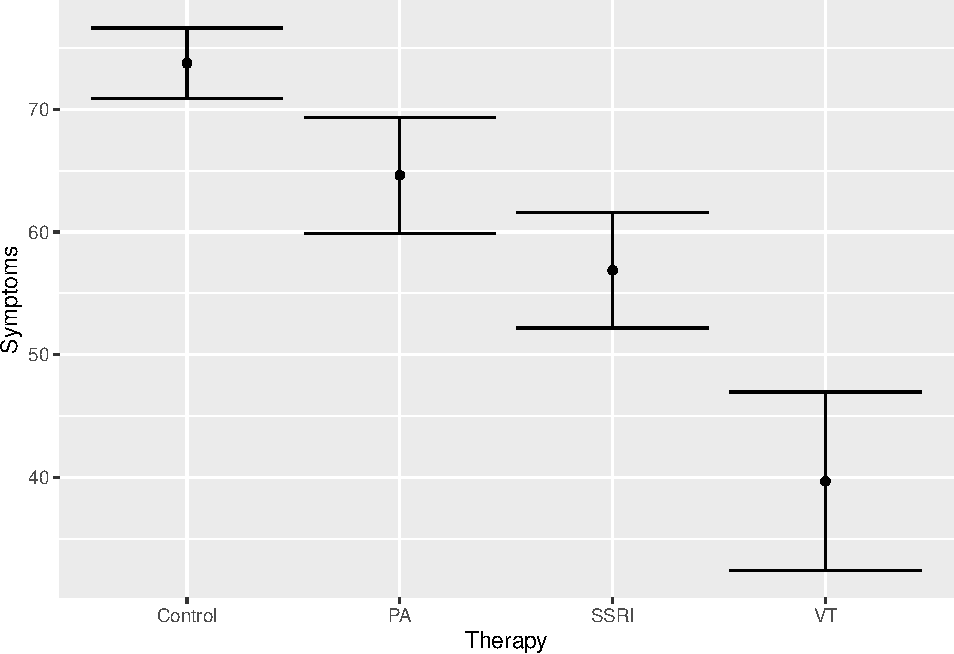
\includegraphics{CFH_R_bookdown_files/figure-latex/unnamed-chunk-304-1.pdf}

Ob sich die numerischen Unterschiede sich auch als signifikant erweisen, prüfen wir mit der ANOVA.

\hypertarget{berechnung-der-anova}{%
\subsection{Berechnung der ANOVA}\label{berechnung-der-anova}}

Die einfaktorielle ANOVA lässt sich in R auf zwei Arten berechnen, die beide zu dem exakt selben Ergebnis kommen.

\begin{itemize}
\tightlist
\item
  eingebaute \texttt{lm()} Funktion gefolgt von \texttt{anova()}
\item
  \texttt{aov\_ez()} Funktion aus dem \texttt{afex} Paket
\end{itemize}

\hypertarget{berechnung-mittels-lm}{%
\subsubsection{\texorpdfstring{Berechnung mittels \texttt{lm()}}{Berechnung mittels lm()}}\label{berechnung-mittels-lm}}

Die \texttt{lm()} Funktion ist eine der gebräuchlichsten in der Statistik überhaupt. Sie ist nach dem \textbf{Allgemeinen linearen Modell} benannt (\textbf{l}inear \textbf{m}odel) und wird beispielsweise auch zur Berechnung der Regression verwendet.

Das lineare Modell wird wie folgt aufgestellt (Formelformat):

\begin{Shaded}
\begin{Highlighting}[]
\NormalTok{mod }\OtherTok{=} \FunctionTok{lm}\NormalTok{(Symptoms }\SpecialCharTok{\textasciitilde{}}\NormalTok{ Therapy, }\AttributeTok{data =}\NormalTok{ therapy)}
\end{Highlighting}
\end{Shaded}

In der Formel steht links immer die AV (Symptoms). Die \texttt{\textasciitilde{}} Symbol heißt soviel wie ``wird vorhergesagt durch''. Auf der rechten Seite steht die UV (Therapy).

Um das Ergebnis der ANOVA (den F-Test) zu erhalten, müssen wir die Funktion \texttt{anova()} auf das erstellte Modell anwenden

\begin{Shaded}
\begin{Highlighting}[]
\FunctionTok{anova}\NormalTok{(mod)}
\end{Highlighting}
\end{Shaded}

\begin{verbatim}
## Analysis of Variance Table
## 
## Response: Symptoms
##           Df Sum Sq Mean Sq F value    Pr(>F)    
## Therapy    3 4242.4 1414.14   8.078 0.0005766 ***
## Residuals 26 4551.6  175.06                      
## ---
## Signif. codes:  0 '***' 0.001 '**' 0.01 '*' 0.05 '.' 0.1 ' ' 1
\end{verbatim}

Wir erhalten den Output der ANOVA mit allen relevanten Zahlen:

\begin{itemize}
\tightlist
\item
  Df = Freiheitsgrade (VORSICHT der F-Test hat 2x df \(\rightarrow\) Zähler-/ und Nennerfreiheitsgrade)
\item
  F-Wert = Teststatistik (könnte in F-Tabelle nachgesehen werden)
\item
  p-Wert \(\rightarrow\) entscheidend dafür, ob ANOVA signifikant ist
\end{itemize}

Die Entscheidungsregel ist uns bereits bekannt: Ist der p-Wert (hier \(p=0.0005766\)) kleiner als \(\alpha=.05\) ist der Test signifikant. Das ist hier der Fall. Das ganze Ergebnis schreibt man i.d.R. wie folgt: \(F_{3,26}=8.08, p<.001\).

\hypertarget{berechnung-mittels-aov_ez}{%
\subsubsection{\texorpdfstring{Berechnung mittels \texttt{aov\_ez()}}{Berechnung mittels aov\_ez()}}\label{berechnung-mittels-aov_ez}}

Die Berechnung mit der \texttt{aov\_ez()} Funktion erfolgt analog, nur wird die Formel etwas anders geschrieben.

Wir legen genau fest, was unsere AV ist \texttt{dv}. Zudem brauchen wir eine Variable, die jede Zeile eindeutig einem Individuum zuordnet \texttt{id}.

Die Faktoren (UVs) werden mit einem der beiden folgenden Argumente angegeben:

\begin{itemize}
\tightlist
\item
  \texttt{between} (Zwischensubjektfaktoren)
\item
  \texttt{within} (Innersubjektfaktoren)
\end{itemize}

Faktoren, die unter \texttt{between} angegeben werden, sind unabhängige Messungen, also Variablen die einen Gruppenvergleich möglich machen. Faktoren, die unter \texttt{within} angegeben werden, sind abhängige Messungen, also beispielsweise mehrere Messzeitpunkte derselben Person.

In unserem Fall liegt ein Gruppenvergleich vor (jede Person hat jeweils nur eine der Therapien erhalten), daher nutzen wir \texttt{between}. Für \texttt{id} nutzen wir einfach die Variable \texttt{ID}, die einen Patientencode für jede Person enthält.

\begin{Shaded}
\begin{Highlighting}[]
\FunctionTok{library}\NormalTok{(afex)}
\NormalTok{mod }\OtherTok{=} \FunctionTok{aov\_ez}\NormalTok{(}\AttributeTok{dv =} \StringTok{"Symptoms"}\NormalTok{, }\AttributeTok{between =} \FunctionTok{c}\NormalTok{(}\StringTok{"Therapy"}\NormalTok{), }\AttributeTok{id =} \StringTok{"ID"}\NormalTok{, }\AttributeTok{data =}\NormalTok{ therapy)}
\NormalTok{mod}
\end{Highlighting}
\end{Shaded}

\begin{verbatim}
## Anova Table (Type 3 tests)
## 
## Response: Symptoms
##    Effect    df    MSE        F  ges p.value
## 1 Therapy 3, 26 175.06 8.08 *** .482   <.001
## ---
## Signif. codes:  0 '***' 0.001 '**' 0.01 '*' 0.05 '+' 0.1 ' ' 1
\end{verbatim}

Wie wir sehen, wird der Schritt des Aufstellens des linearen Modells hier übersprungen und direkt die ANOVA (F-Test) gerechnet.
Das Ergebnise ist jedoch identisch.

Falls im Datensatz keine \texttt{id} Variable enthalten ist, lässt sich diese leicht erstellen, indem wir einfach jeder Person Ihre Position im Datensatz als Namen geben:

\begin{Shaded}
\begin{Highlighting}[]
\NormalTok{therapy}\SpecialCharTok{$}\NormalTok{id }\OtherTok{=} \FunctionTok{rownames}\NormalTok{(therapy)}

\FunctionTok{head}\NormalTok{(therapy)}
\end{Highlighting}
\end{Shaded}

\begin{verbatim}
##   ID Therapy Symptoms  Diagnosis id
## 1  1    SSRI       46 Depression  1
## 2  2    SSRI       69      Angst  2
## 3  3    SSRI       39 Depression  3
## 4  4    SSRI       80      Angst  4
## 5  5    SSRI       50 Depression  5
## 6  6    SSRI       63      Angst  6
\end{verbatim}

\hypertarget{interpretation}{%
\subsection{Interpretation}\label{interpretation}}

Die ANOVA ist in unserem Beispiel signifikant geworden. Dies gibt uns die Information, dass der Faktor Therapie einen signifikanten Anteil der Varianz unserer AV (Symptoms) erklären kann. Anders gesagt: Es scheinen hinsichtlich der Symptomatik Unterschiede zwischen den Gruppen zu bestehen.

Aus dem signifikanten Ergebnis der ANOVA können wir jedoch nicht erkennen, \textbf{zwischen welchen der Gruppen} die Unterschiede genau bestehen. Wir wissen es gibt einen Effekt, nur nicht wo er liegt.

Aus diesem Grund folgt auf die Berechnung der ANOVA ein zweiter Schritt, um mittels \textbf{paarweisen Vergleichen} zu prüfen, wo die Unterschiede liegen. Diese paarweisen Vergleiche nennt man auch Post-hoc Tests

\hypertarget{post-hoc-tests}{%
\subsection{Post-hoc Tests}\label{post-hoc-tests}}

Post-hoc Tests erlauben uns genau zu sehen, welche der Stufen unserer UV sich unterscheiden. In diesem Sinne sind sie nichts anderes als nachgeschaltete t-Tests, die 2 Gruppen miteinander vergleichen.

Wir berechnen Post-hoc Tests mit der \texttt{emmeans()} Funktion aus dem gleichnamigen \texttt{emmeans} Paket. Die Abkürzung emmeans bedeuted ``estimated marginal means'', was soviel bedeutet wie die Mittelwerte des Modells innerhalb der Faktorstufen zu vergleichen.

Die \texttt{emmeans()} Funktion kann man sowohl nach der ANOVA mit \texttt{lm()} als auch nach der ANOVA mit \texttt{aov\_ez()} verwenden.

\begin{Shaded}
\begin{Highlighting}[]
\FunctionTok{library}\NormalTok{(emmeans)}
\FunctionTok{emmeans}\NormalTok{(mod, pairwise }\SpecialCharTok{\textasciitilde{}}\NormalTok{ Therapy)}
\end{Highlighting}
\end{Shaded}

\begin{verbatim}
## $emmeans
##  Therapy emmean   SE df lower.CL upper.CL
##  Control   73.8 4.68 26     64.1     83.4
##  PA        64.6 4.68 26     55.0     74.2
##  SSRI      56.9 4.68 26     47.3     66.5
##  VT        39.7 5.40 26     28.6     50.8
## 
## Confidence level used: 0.95 
## 
## $contrasts
##  contrast       estimate   SE df t.ratio p.value
##  Control - PA       9.12 6.62 26   1.379  0.5230
##  Control - SSRI    16.88 6.62 26   2.551  0.0752
##  Control - VT      34.08 7.15 26   4.770  0.0003
##  PA - SSRI          7.75 6.62 26   1.171  0.6497
##  PA - VT           24.96 7.15 26   3.493  0.0088
##  SSRI - VT         17.21 7.15 26   2.408  0.1004
## 
## P value adjustment: tukey method for comparing a family of 4 estimates
\end{verbatim}

Mit dem \texttt{pairwise} Argument sagen wir der \texttt{emmeans()} Funktion zwischen welchen Gruppen die Mittelwertsvergleiche durchgeführt werden sollen.

Der Output der \texttt{emmeans()} Funktion hat 2 Teile

\begin{itemize}
\tightlist
\item
  \$emmeans (oberer Teil: hier werden praktischerweise die verglichenen Mittelwerte noch einmal ausgerechnet)
\item
  \$contrasts (unterer Teil: hier werden die Ergebnisse der Post-hoc Tests gezeigt)
\end{itemize}

Die Interpretation des Ergebnisses ist uns bereits bekannt. Jeder Vergleich erhält einen t-Wert und einen p-Wert, anhand dessen wir ablesen können, ob der Gruppenunterschied signifikant war.

Der Mittelwert der Gruppe VT war signifikant niedriger als der in der Kontrollgruppe \((t_{26}=4.77,p=.0003)\) und als der in der PA Gruppe \((t_{26}=3.49,p=.0088)\). Die anderen Vergleiche waren nicht signifikant.

\hypertarget{korrektur-fuxfcr-multiples-testen}{%
\subsubsection{Korrektur für multiples Testen}\label{korrektur-fuxfcr-multiples-testen}}

Nun haben wir im Abschnitt über die \(\alpha\)-Fehler Kumulierung bereits erfahren, dass das Durchführen vieler Vergleiche problematisch sein kann, da es die Wahrscheinlichkeit erhöht, einen Fehler 1. Art zu begehen.

Post-hoc Tests lösen dieses Problem durch eine Korrektur des p-Werts. Je mehr Vergleiche gemacht werden, desto mehr wird er nach oben korrigiert. Automatisch wendet \texttt{emmeans()} die sogenannte Tukey-Korrektur an (ganz unten im Output sichtbar).

Zwei weitere Korrekturen sind gängig, die etwas strengere Bonferroni-Korrektur und die etwas weniger strenge Benjamini-Hochberg Korrektur (auch false-dicovery-rate Korrektur - FDR genannt).

Wollen wir die Korrekturmethode ändern, lässt sich das leicht über das \texttt{adjust} Argument erreichen:

\begin{Shaded}
\begin{Highlighting}[]
\FunctionTok{emmeans}\NormalTok{(mod, pairwise }\SpecialCharTok{\textasciitilde{}}\NormalTok{ Therapy, }\AttributeTok{adjust =} \StringTok{"bonferroni"}\NormalTok{)}
\end{Highlighting}
\end{Shaded}

\begin{verbatim}
## $emmeans
##  Therapy emmean   SE df lower.CL upper.CL
##  Control   73.8 4.68 26     64.1     83.4
##  PA        64.6 4.68 26     55.0     74.2
##  SSRI      56.9 4.68 26     47.3     66.5
##  VT        39.7 5.40 26     28.6     50.8
## 
## Confidence level used: 0.95 
## 
## $contrasts
##  contrast       estimate   SE df t.ratio p.value
##  Control - PA       9.12 6.62 26   1.379  1.0000
##  Control - SSRI    16.88 6.62 26   2.551  0.1019
##  Control - VT      34.08 7.15 26   4.770  0.0004
##  PA - SSRI          7.75 6.62 26   1.171  1.0000
##  PA - VT           24.96 7.15 26   3.493  0.0104
##  SSRI - VT         17.21 7.15 26   2.408  0.1405
## 
## P value adjustment: bonferroni method for 6 tests
\end{verbatim}

Wir sehen, dass die etwas strengere Bonferroni-Korrektur die p-Werte vergleichsweise höher werden lässt, als mit der Tukey-Korrektur. Es ist also für den p-Wert schwieriger, unter das Signifikanznivea \(\alpha=.05\) zu kommen.

Mit der Benjamini-Hochberg Korrektur sind die Anpassungen weniger streng:

\begin{Shaded}
\begin{Highlighting}[]
\FunctionTok{emmeans}\NormalTok{(mod, pairwise }\SpecialCharTok{\textasciitilde{}}\NormalTok{ Therapy, }\AttributeTok{adjust =} \StringTok{"fdr"}\NormalTok{)}
\end{Highlighting}
\end{Shaded}

\begin{verbatim}
## $emmeans
##  Therapy emmean   SE df lower.CL upper.CL
##  Control   73.8 4.68 26     64.1     83.4
##  PA        64.6 4.68 26     55.0     74.2
##  SSRI      56.9 4.68 26     47.3     66.5
##  VT        39.7 5.40 26     28.6     50.8
## 
## Confidence level used: 0.95 
## 
## $contrasts
##  contrast       estimate   SE df t.ratio p.value
##  Control - PA       9.12 6.62 26   1.379  0.2155
##  Control - SSRI    16.88 6.62 26   2.551  0.0340
##  Control - VT      34.08 7.15 26   4.770  0.0004
##  PA - SSRI          7.75 6.62 26   1.171  0.2520
##  PA - VT           24.96 7.15 26   3.493  0.0052
##  SSRI - VT         17.21 7.15 26   2.408  0.0351
## 
## P value adjustment: fdr method for 6 tests
\end{verbatim}

\hypertarget{mehrfaktorielle-anova}{%
\section{Mehrfaktorielle ANOVA}\label{mehrfaktorielle-anova}}

Mit der ANOVA haben wir die Möglichkeit, die Effekte mehrere UVs (Faktoren) auf die AV zu untersuchen.

Wir prüfen dann letztlich 3 Hypothesen (bei 2 UVs)

\begin{itemize}
\tightlist
\item
  Haupteffekt des 1. Faktors
\item
  Haupteffekt des 2. Faktors
\item
  Interaktionseffekt beider Faktoren
\end{itemize}

In unserem Beispiel könnte es interessant sein, zusätzlich zur erhaltenen Therapie zu berücksichtigen, welche Diagnose die Patienten hatten.

Unsere Fragestellung würde sich um 2 weitere Aspekte erweitern:

\begin{enumerate}
\def\labelenumi{\arabic{enumi}.}
\tightlist
\item
  \emph{Nach welcher Therapie haben die Patient:innen die schwächsten Symptome?} (hatten wir bereits - Haupteffekt Therapie)
\item
  \emph{Welche Diagnose hatte die schwächsten Symptome?} (Haupteffekt Diagnose)
\item
  \emph{Gibt es, je nachdem welche Diagnose die Patienten hatten, Unterschiede in der Wirksamkeit der Therapie?} (Interaktioniseffekt)
\end{enumerate}

\hypertarget{deskriptive-einordnung-5}{%
\subsection{Deskriptive Einordnung}\label{deskriptive-einordnung-5}}

Zunächst können wir uns die Deskriptivstatistiken innerhalb der Gruppen einmal anschauen:

\begin{Shaded}
\begin{Highlighting}[]
\NormalTok{psych}\SpecialCharTok{::}\FunctionTok{describeBy}\NormalTok{(Symptoms }\SpecialCharTok{\textasciitilde{}}\NormalTok{ Therapy }\SpecialCharTok{*}\NormalTok{ Diagnosis, }\AttributeTok{data =}\NormalTok{ therapy)}
\end{Highlighting}
\end{Shaded}

\begin{verbatim}
## 
##  Descriptive statistics by group 
## Therapy: Control
## Diagnosis: Angst
##          vars n mean   sd median trimmed  mad min max range  skew kurtosis   se
## Symptoms    1 5 71.2 8.41     70    71.2 7.41  59  82    23 -0.17    -1.56 3.76
## ------------------------------------------------------------ 
## Therapy: PA
## Diagnosis: Angst
##          vars n mean    sd median trimmed   mad min max range skew kurtosis
## Symptoms    1 4   66 18.57   63.5      66 17.05  47  90    43 0.25    -2.01
##            se
## Symptoms 9.28
## ------------------------------------------------------------ 
## Therapy: SSRI
## Diagnosis: Angst
##          vars n  mean    sd median trimmed  mad min max range  skew kurtosis
## Symptoms    1 4 65.75 12.09     66   65.75 12.6  51  80    29 -0.04    -1.96
##            se
## Symptoms 6.05
## ------------------------------------------------------------ 
## Therapy: VT
## Diagnosis: Angst
##          vars n mean    sd median trimmed   mad min max range skew kurtosis  se
## Symptoms    1 2 24.5 13.44   24.5    24.5 14.08  15  34    19    0    -2.75 9.5
## ------------------------------------------------------------ 
## Therapy: Control
## Diagnosis: Depression
##          vars n mean   sd median trimmed mad min max range  skew kurtosis se
## Symptoms    1 3   78 6.93     82      78   0  70  82    12 -0.38    -2.33  4
## ------------------------------------------------------------ 
## Therapy: PA
## Diagnosis: Depression
##          vars n  mean   sd median trimmed  mad min max range skew kurtosis   se
## Symptoms    1 4 63.25 8.26     62   63.25 7.41  55  74    19 0.27    -2.02 4.13
## ------------------------------------------------------------ 
## Therapy: SSRI
## Diagnosis: Depression
##          vars n mean   sd median trimmed  mad min max range skew kurtosis   se
## Symptoms    1 4   48 7.53     48      48 8.15  39  57    18    0    -1.98 3.76
## ------------------------------------------------------------ 
## Therapy: VT
## Diagnosis: Depression
##          vars n  mean    sd median trimmed  mad min max range skew kurtosis
## Symptoms    1 4 47.25 15.52     45   47.25 12.6  31  68    37  0.3     -1.9
##            se
## Symptoms 7.76
\end{verbatim}

Der \texttt{*} zwischen den Faktoren bedeutet ``Interaktion'' und führt dazu, dass alle Stufenkombinationen der beiden Variablen exploriert werden.

Die Gruppenunterschiede lassen sich auch graphisch gut darstellen:

\begin{Shaded}
\begin{Highlighting}[]
\FunctionTok{ggplot}\NormalTok{(}\AttributeTok{data =}\NormalTok{ therapy, }\FunctionTok{aes}\NormalTok{(}\AttributeTok{x =}\NormalTok{ Therapy, }\AttributeTok{y =}\NormalTok{ Symptoms, }\AttributeTok{colour =}\NormalTok{ Diagnosis)) }\SpecialCharTok{+}
  \FunctionTok{stat\_summary}\NormalTok{(}\AttributeTok{fun.data =}\NormalTok{ mean\_se,  }\AttributeTok{geom =} \StringTok{"errorbar"}\NormalTok{) }\SpecialCharTok{+}
  \FunctionTok{stat\_summary}\NormalTok{(}\AttributeTok{geom =} \StringTok{"point"}\NormalTok{, }\AttributeTok{fun =}\NormalTok{ mean) }
\end{Highlighting}
\end{Shaded}

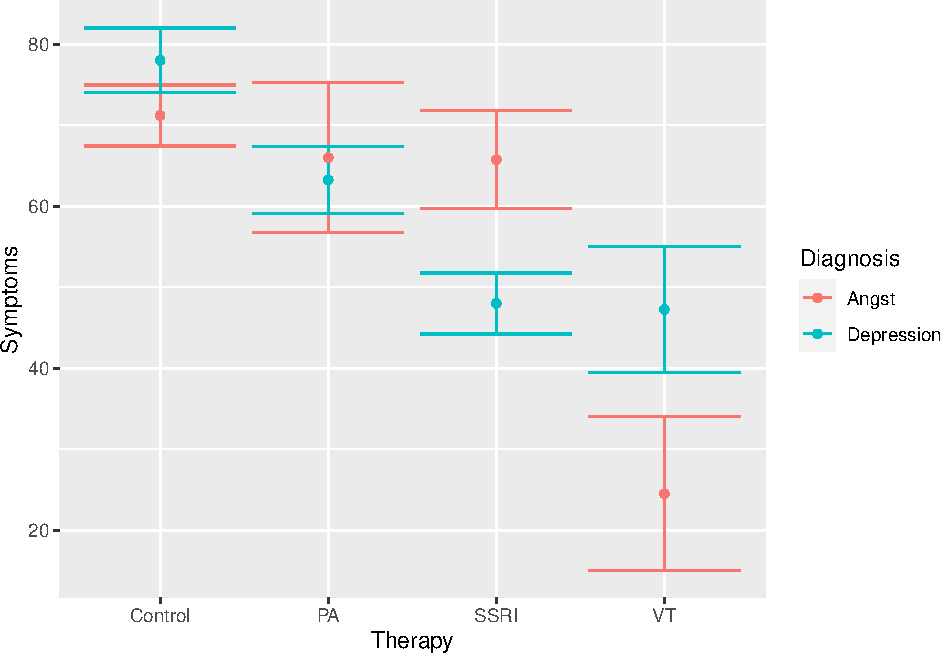
\includegraphics{CFH_R_bookdown_files/figure-latex/unnamed-chunk-313-1.pdf}

\hypertarget{berechnung-der-anova-1}{%
\subsection{Berechnung der ANOVA}\label{berechnung-der-anova-1}}

\hypertarget{berechnung-mittels-lm-1}{%
\subsubsection{\texorpdfstring{Berechnung mittels \texttt{lm()}}{Berechnung mittels lm()}}\label{berechnung-mittels-lm-1}}

Die Vorgehensweise ist dieselbe wie bei der einfaktoriellen ANOVA. Die Formel wird lediglich durch die Interaktion mit der 2. UV erweitert.

\begin{Shaded}
\begin{Highlighting}[]
\NormalTok{mod }\OtherTok{=} \FunctionTok{lm}\NormalTok{(Symptoms }\SpecialCharTok{\textasciitilde{}}\NormalTok{ Therapy }\SpecialCharTok{*}\NormalTok{ Diagnosis, }\AttributeTok{data =}\NormalTok{ therapy)}
\FunctionTok{anova}\NormalTok{(mod)}
\end{Highlighting}
\end{Shaded}

\begin{verbatim}
## Analysis of Variance Table
## 
## Response: Symptoms
##                   Df Sum Sq Mean Sq F value    Pr(>F)    
## Therapy            3 4242.4 1414.14  9.9411 0.0002439 ***
## Diagnosis          1    0.6    0.60  0.0042 0.9487141    
## Therapy:Diagnosis  3 1421.4  473.81  3.3308 0.0381543 *  
## Residuals         22 3129.6  142.25                      
## ---
## Signif. codes:  0 '***' 0.001 '**' 0.01 '*' 0.05 '.' 0.1 ' ' 1
\end{verbatim}

Der Output der ANOVA erweitert sich im Vergleich zur einfaktoriellen ANOVA um 2 Zeilen. Die mit \texttt{Therapy} und \texttt{Diagnosis} betitelten Zeilen sind die Haupteffekte. Die 3. Zeile \texttt{Therapy:Diagnosis} ist der Interaktionseffekt.

Da wir mit der 2-faktoriellen ANOVA letztlich 3 Hypothesen prüfen, gibt es auch 3 p-Werte, die alle entweder signifikante oder nicht-signifikant sein können.

\hypertarget{berechnung-mittels-aov_ez-1}{%
\subsubsection{\texorpdfstring{Berechnung mittels \texttt{aov\_ez()}}{Berechnung mittels aov\_ez()}}\label{berechnung-mittels-aov_ez-1}}

Auch für die \texttt{aov\_ez()} Funktion ähnelt das Vorgehen dem der einfaktoriellen ANOVA. Hier wird die Liste der UVs lediglich um den 2. Faktor erweitert, die Interaktion wird automatisch mitberechnet. Das Ergebnis ist analog zur \texttt{lm()} Funktion.

\begin{Shaded}
\begin{Highlighting}[]
\FunctionTok{library}\NormalTok{(afex)}
\NormalTok{mod }\OtherTok{=} \FunctionTok{aov\_ez}\NormalTok{(}\AttributeTok{dv =} \StringTok{"Symptoms"}\NormalTok{, }\AttributeTok{between =} \FunctionTok{c}\NormalTok{(}\StringTok{"Therapy"}\NormalTok{, }\StringTok{"Diagnosis"}\NormalTok{), }\AttributeTok{id =} \StringTok{"ID"}\NormalTok{, }\AttributeTok{data =}\NormalTok{ therapy)}
\NormalTok{mod}
\end{Highlighting}
\end{Shaded}

\begin{verbatim}
## Anova Table (Type 3 tests)
## 
## Response: Symptoms
##              Effect    df    MSE         F  ges p.value
## 1           Therapy 3, 22 142.25 11.60 *** .613   <.001
## 2         Diagnosis 1, 22 142.25      0.25 .011    .621
## 3 Therapy:Diagnosis 3, 22 142.25    3.33 * .312    .038
## ---
## Signif. codes:  0 '***' 0.001 '**' 0.01 '*' 0.05 '+' 0.1 ' ' 1
\end{verbatim}

\hypertarget{interpretation-1}{%
\subsection{Interpretation}\label{interpretation-1}}

Die beiden Haupteffekte und der Interaktionseffekt können einzeln interpretiert werden. Wir gehen der Reihe nach:

\hypertarget{haupteffekt-1}{%
\subsubsection{Haupteffekt 1}\label{haupteffekt-1}}

Der Haupteffekt von \texttt{Therapy} spiegelt im Wesentlichen das Ergebnis wieder, welches wir bereits von der einfaktoriellen ANOVA kennen. Es handelt sich um den Effekt der Therapie, wenn man den Effekt der 2. UV (Diagnosis) außer Acht lässt.

Der Haupteffekt ist signifikant bei \(F_{(3,22)}=9.94, p<.001\). Wir können schlussfolgern, dass es einen Unterschied zwischen den Diagnosen gibt. Wo die Unterschiede genau liegenm, können wir mit den Post-hoc Tests bestimmen, wie oben bereits geschehen.

\hypertarget{haupteffekt-2}{%
\subsubsection{Haupteffekt 2}\label{haupteffekt-2}}

Der Haupteffekt von \texttt{Diagnosis} ist nichts anderes als ein unabhängiger t-Test. Es handelt sich um den Effekt der Diagnose, wenn man den Effekt der 1. UV (Therapy) außer Acht lässt. Dieser Haupteffekt ist nicht signifikant \(F_{(1,22)}=0.004, p<.949\). Über alle Therapien hinweg scheint es keinen Unterschied in der Symptomatik der Patient:innen mit Depressionen und Angststörungen zu geben.

\hypertarget{interaktionseffekt}{%
\subsubsection{Interaktionseffekt}\label{interaktionseffekt}}

Der Interaktionseffekt von \texttt{Therapy\ *\ Diagnosis} prüft, ob der Effekt der Therapie in beiden Diagnosen unterschiedlich wirkt.
Er ist somit eine Möglichkeit den ``kombinierten Effekt'' der beiden Variablen zu prüfen.

Der Interaktionseffekt ist signifikant \(F_{(3,22)}=3.33, p<.038\). Entsprechend scheinen die Patient:innen nach den Therapien unterschiedlich wenige Symptome zu haben, je nachdem welche Diagnose sie hatten.

Um diesen Effekt inhaltlich zu verstehen, empfiehlt sich ein Blick auf die Graphik, in Kombination mit Post-Hoc Tests.

\hypertarget{post-hoc-tests-1}{%
\subsection{Post-hoc Tests}\label{post-hoc-tests-1}}

Zum Verständnis der Effekte führen wir Post-Hoc Tests durch. Allerdings wollen wir uns den Effekt der Therapie diesmal getrennt für die Diagnosen ansehen.

\begin{Shaded}
\begin{Highlighting}[]
\FunctionTok{library}\NormalTok{(emmeans)}
\FunctionTok{emmeans}\NormalTok{(mod, pairwise }\SpecialCharTok{\textasciitilde{}}\NormalTok{ Therapy}\SpecialCharTok{|}\NormalTok{Diagnosis)}
\end{Highlighting}
\end{Shaded}

\begin{verbatim}
## $emmeans
## Diagnosis = Angst:
##  Therapy emmean   SE df lower.CL upper.CL
##  Control   71.2 5.33 22    60.14     82.3
##  PA        66.0 5.96 22    53.63     78.4
##  SSRI      65.8 5.96 22    53.38     78.1
##  VT        24.5 8.43 22     7.01     42.0
## 
## Diagnosis = Depression:
##  Therapy emmean   SE df lower.CL upper.CL
##  Control   78.0 6.89 22    63.72     92.3
##  PA        63.2 5.96 22    50.88     75.6
##  SSRI      48.0 5.96 22    35.63     60.4
##  VT        47.2 5.96 22    34.88     59.6
## 
## Confidence level used: 0.95 
## 
## $contrasts
## Diagnosis = Angst:
##  contrast       estimate    SE df t.ratio p.value
##  Control - PA       5.20  8.00 22   0.650  0.9144
##  Control - SSRI     5.45  8.00 22   0.681  0.9031
##  Control - VT      46.70  9.98 22   4.680  0.0006
##  PA - SSRI          0.25  8.43 22   0.030  1.0000
##  PA - VT           41.50 10.33 22   4.018  0.0030
##  SSRI - VT         41.25 10.33 22   3.994  0.0032
## 
## Diagnosis = Depression:
##  contrast       estimate    SE df t.ratio p.value
##  Control - PA      14.75  9.11 22   1.619  0.3889
##  Control - SSRI    30.00  9.11 22   3.293  0.0162
##  Control - VT      30.75  9.11 22   3.376  0.0134
##  PA - SSRI         15.25  8.43 22   1.808  0.2962
##  PA - VT           16.00  8.43 22   1.897  0.2580
##  SSRI - VT          0.75  8.43 22   0.089  0.9997
## 
## P value adjustment: tukey method for comparing a family of 4 estimates
\end{verbatim}

Wir sehen, dass die Symptome nach SSRI insbesondere in der Gruppe der depressiven Patient:innen reduziert sind. Zudem sind die Symtome nach der VT deutlich reduziert (insbesondere bei Angststörungen).

Dies führt dazu, dass die VT (in dieser Stichprobe) in der Behandlung von Angststörungen der Kontrollgruppe \((t_{(22)}=4.68, p<.001)\), der Psychoanalyse \((t_{(22)}=4.02, p=.003)\) und den SSRI \((t_{(22)}=3.99, p=.003)\) überlegen war. In der Behandlung von Angststörungen waren sowohl SSRI \((t_{(22)}=3.29, p=.016)\) als auch VT \((t_{(22)}=3.38, p=.013)\) besser als die Kontrollgruppe, unterschieden sich jedoch nicht signifikant von der Psychoanalyse und auch nicht voneinander.

\hypertarget{pruxfcfen-der-voraussetzungen-von-anovas}{%
\section{Prüfen der Voraussetzungen von ANOVAs}\label{pruxfcfen-der-voraussetzungen-von-anovas}}

Wie alle statistischen Modelle haben ANOVAs eine Reihe von Annahmen, die für gültige Schlussfolgerungen gelten sollten. Diese Annahmen sind:

\begin{enumerate}
\def\labelenumi{\arabic{enumi}.}
\item
  \textbf{Beobachtungen sind i.i.d.:} i.i.d. steht für ``unabhängig und identisch verteilt''. Unabhängig bedeutet, dass die bedingten Beobachtungen (d.h. Residuen) unabhängig voneinander sind (d.h. das Wissen des Wertes eines Residuums erlaubt keine Rückschlüsse auf den Wert eines anderen Residuums). Identisch verteilt bedeutet, dass alle Beobachtungen durch denselben Daten-generierenden Prozess erzeugt werden.
\item
  \textbf{Homogenität der Varianzen:} Die Varianzen über alle Gruppen (Zellen) der zwischen-Subjekt-Effekte sind gleich.
\item
  \textbf{Sphärizität:} Bei innerhalb-Subjekt-Effekten ist die Sphärizität die Bedingung, dass die Varianzen der Unterschiede zwischen allen möglichen Paaren von innerhalb-Subjekt-Bedingungen (d.h. Levels der unabhängigen Variablen) gleich sind. Dies kann als eine innerhalb-Subjekt-Version der Homogenität der Varianzen-Annahme betrachtet werden.
\item
  \textbf{Normalverteilung der Residuen:} Die Fehler, die für die Schätzung des Fehlerterms (MSE) verwendet werden, sind normalverteilt.
\end{enumerate}

Die wichtigste Annahme ist im Allgemeinen die i.i.d.-Annahme (d.h. wenn sie nicht erfüllt ist, sind die Schlussfolgerungen wahrscheinlich ungültig), insbesondere der unabhängige Teil. Diese Annahme kann nicht empirisch getestet werden, sondern muss auf konzeptuellen oder logischen Gründen beruhen. Zum Beispiel stammen in einem idealen vollständig zwischen den Probanden durchgeführten Design jede Beobachtung von einem anderen Probanden, der zufällig aus einer Population ausgewählt wird, so dass wir wissen, dass alle Beobachtungen unabhängig sind. Oft sammeln wir jedoch mehrere Beobachtungen von demselben Probanden in einem innerhalb der Probanden oder wiederholten Messungen-Design. Um sicherzustellen, dass die i.i.d.-Annahme in diesem Fall erfüllt ist, müssen wir eine ANOVA mit innerhalb der Probanden Faktoren angeben. Wenn wir jedoch einen Datensatz mit mehreren Quellen von Nicht-Unabhängigkeit haben - wie Teilnehmern und Items - können ANOVA-Modelle nicht verwendet werden, sondern wir müssen ein gemischtes Modell verwenden.

Die anderen Annahmen können empirisch getestet werden, entweder graphisch oder mit statistischen Annahmetests. Es gibt jedoch unterschiedliche Meinungen darüber, wie nützlich statistische Annahmetests sind, wenn sie automatisch für jede ANOVA durchgeführt werden. Obwohl dies in einigen Statistikbüchern vertreten wird, besteht die Gefahr, dass die statistische Analyse auf ein ``Kochbuch'' oder ``Flussdiagramm'' reduziert wird. Die Datenanalyse in der Realität ist oft komplexer als solche einfachen Regeln. Es ist daher oft produktiver, die Daten mit Hilfe von deskriptiven Statistiken und grafischen Darstellungen zu erkunden. Diese Datenexploration sollte es ermöglichen, zu beurteilen, ob die anderen ANOVA-Annahmen in ausreichendem Maße erfüllt sind. Zum Beispiel ermöglicht es das Plotten der ANOVA-Ergebnisse mit afex\_plot und einer vernünftigen Darstellung der einzelnen Datenpunkte oft, sowohl die Homogenität der Varianz als auch die Normalverteilung der Residuenannahme zu beurteilen.

Lassen Sie uns nun alle drei empirisch testbaren Annahmen im Detail betrachten. ANOVAs sind oft robust gegen leichte Verletzungen der Annahme der Homogenität der Varianzen. Wenn diese Annahme jedoch deutlich verletzt ist, haben wir etwas Wichtiges über die Daten gelernt, nämlich Varianzheterogenität, die weitere Untersuchungen erfordert. Einige weitere statistische Lösungen werden unten diskutiert.

Wenn das Hauptziel einer ANOVA darin besteht, zu sehen, ob bestimmte Effekte signifikant sind oder nicht, dann ist die Annahme der Normalverteilung der Residuen nur für kleine Stichproben erforderlich, dank des zentralen Grenzwertsatzes. Wie von Lumley et al.~(2002) gezeigt, sind selbst extreme Verletzungen der Normalitätsannahmen bei Stichproben von ein paar hundert Probanden unproblematisch. Daher sind leichte Verletzungen dieser Annahme unproblematisch.

Eine angemessene explorative Datenanalyse oft besser ist als die blindes Anwenden von statistischen Annahmetests. Dennoch sind Annahmetests natürlich ein wichtiges Werkzeug im statistischen Werkzeugkasten und können in vielen Situationen hilfreich sein.

\hypertarget{testen-der-empirisch-testbaren-annahmen}{%
\subsection{Testen der empirisch testbaren Annahmen}\label{testen-der-empirisch-testbaren-annahmen}}

\texttt{afex}verfügt über eine Reihe von integrierten Funktionen, um bei der Überprüfung der Annahmen des ANOVA-Designs zu helfen.

\begin{itemize}
\tightlist
\item
  Die Varianzen über alle Gruppen (Zellen) der zwischen-subjektiven Effekte sind gleich. Dies kann mit performance::check\_homogeneity() getestet werden.
\item
  Sphärizität: Für innerhalb-subjektive Effekte ist die Sphärizität die Bedingung, bei der die Varianzen der Unterschiede zwischen allen möglichen Paaren von innerhalb-subjektiven Bedingungen (d.h. Stufen der unabhängigen Variable) gleich sind. Dies kann als eine innerhalb-subjektive Version der Homogenität der Varianzen betrachtet werden und kann mit performance::check\_sphericity() getestet werden.
\item
  Normalität der Residuen: Die für die Schätzung des Fehlerterms (MSE) verwendeten Fehler sind normal verteilt. Dies kann mit performance::check\_normality() abgeleitet werden.
\end{itemize}

\begin{Shaded}
\begin{Highlighting}[]
\FunctionTok{library}\NormalTok{(afex)}
\FunctionTok{library}\NormalTok{(performance) }\CommentTok{\# für die Voraussetzungsprüfung}
\end{Highlighting}
\end{Shaded}

\hypertarget{homogenituxe4t-der-varianzen}{%
\subsection{Homogenität der Varianzen:}\label{homogenituxe4t-der-varianzen}}

Diese Annahme besagt für Zwischen-Gruppen-Designs, dass die Fehler innerhalb der Gruppen eine gemeinsame Varianz um den Mittelwert der Gruppe aufweisen.

\hypertarget{test}{%
\subsubsection{Test}\label{test}}

Dies kann mit dem Levene-Test getestet werden:

\begin{Shaded}
\begin{Highlighting}[]
\FunctionTok{data}\NormalTok{(obk.long, }\AttributeTok{package =} \StringTok{"afex"}\NormalTok{)}

\NormalTok{mod }\OtherTok{\textless{}{-}} \FunctionTok{aov\_ez}\NormalTok{(}\StringTok{"id"}\NormalTok{, }\StringTok{"value"}\NormalTok{, obk.long, }
             \AttributeTok{between =} \FunctionTok{c}\NormalTok{(}\StringTok{"treatment"}\NormalTok{, }\StringTok{"gender"}\NormalTok{))}
\end{Highlighting}
\end{Shaded}

\begin{verbatim}
## Warning: More than one observation per design cell, aggregating data using `fun_aggregate = mean`.
## To turn off this warning, pass `fun_aggregate = mean` explicitly.
\end{verbatim}

\begin{verbatim}
## Contrasts set to contr.sum for the following variables: treatment, gender
\end{verbatim}

\begin{Shaded}
\begin{Highlighting}[]
\FunctionTok{check\_homogeneity}\NormalTok{(mod)}
\end{Highlighting}
\end{Shaded}

\begin{verbatim}
## OK: There is not clear evidence for different variances across groups (Levene's Test, p = 0.350).
\end{verbatim}

Diese Ergebnisse deuten darauf hin, dass die Homogenität nicht signifikant verletzt ist.

\hypertarget{mauxdfnahmen-wenn-vorraussetzung-verletzt}{%
\subsubsection{Maßnahmen wenn Vorraussetzung verletzt}\label{mauxdfnahmen-wenn-vorraussetzung-verletzt}}

ANOVAs sind im Allgemeinen robust gegenüber ``leichter'' Heteroskedastizität, aber es gibt verschiedene andere Methoden (die in \texttt{afex} nicht verfügbar sind), um robuste Fehlerabschätzungen zu erhalten.

Eine weitere Alternative besteht darin, diese Annahme ganz aufzugeben und Permutationstests (z.B. mit \texttt{permuco}) oder Bootstrap-Schätzungen (z.B. mit \texttt{boot}) zu verwenden.

\hypertarget{sphuxe4rizituxe4t}{%
\subsection{Sphärizität:}\label{sphuxe4rizituxe4t}}

\hypertarget{test-1}{%
\subsubsection{Test}\label{test-1}}

Wir können check\_sphericity() verwenden, um den Mauchly-Test auf Sphärizität durchzuführen:

\begin{Shaded}
\begin{Highlighting}[]
\FunctionTok{data}\NormalTok{(}\StringTok{"fhch2010"}\NormalTok{, }\AttributeTok{package =} \StringTok{"afex"}\NormalTok{)}

\NormalTok{mod }\OtherTok{\textless{}{-}} \FunctionTok{aov\_ez}\NormalTok{(}\StringTok{"id"}\NormalTok{, }\StringTok{"log\_rt"}\NormalTok{, fhch2010,}
             \AttributeTok{between =} \StringTok{"task"}\NormalTok{, }
             \AttributeTok{within =} \FunctionTok{c}\NormalTok{(}\StringTok{"density"}\NormalTok{, }\StringTok{"frequency"}\NormalTok{, }\StringTok{"length"}\NormalTok{, }\StringTok{"stimulus"}\NormalTok{))}
\end{Highlighting}
\end{Shaded}

\begin{verbatim}
## Warning: More than one observation per design cell, aggregating data using `fun_aggregate = mean`.
## To turn off this warning, pass `fun_aggregate = mean` explicitly.
\end{verbatim}

\begin{verbatim}
## Contrasts set to contr.sum for the following variables: task
\end{verbatim}

\begin{Shaded}
\begin{Highlighting}[]
\FunctionTok{check\_sphericity}\NormalTok{(mod)}
\end{Highlighting}
\end{Shaded}

\begin{verbatim}
## Warning in summary.Anova.mlm(object$Anova, multivariate = FALSE): HF eps > 1
## treated as 1
\end{verbatim}

\begin{verbatim}
## Warning: Sphericity violated for: 
##  - length:stimulus (p = 0.021)
##  - task:length:stimulus (p = 0.021).
\end{verbatim}

Wir können sehen, dass beide Fehlerterme der Länge:Reiz und Aufgabe:Länge:Reiz-Interaktionen die Annahme der Sphärizität bei \(p = 0.021\) signifikant verletzen. Beachten Sie, dass Aufgabe als Faktor zwischen den Probanden gilt und dass beide Interaktionsterme denselben Fehlerterm teilen!

\hypertarget{mauxdfnahmen-wenn-vorraussetzung-verletzt-1}{%
\subsubsection{Maßnahmen wenn Vorraussetzung verletzt}\label{mauxdfnahmen-wenn-vorraussetzung-verletzt-1}}

Für ANOVA-Tabellen kann eine Korrektur der Freiheitsgrade verwendet werden - afex bietet sowohl die Greenhouse-Geisser (die standardmäßig verwendet wird) als auch die Hyunh-Feldt-Korrekturen an.
Für Nachfolgekontraste mit emmeans kann ein multivariates Modell verwendet werden, das keine Sphärizität annimmt (dies wird seit afex 1.0 standardmäßig verwendet).

Beide können global festgelegt werden mit:

\begin{Shaded}
\begin{Highlighting}[]
\FunctionTok{afex\_options}\NormalTok{(}
  \AttributeTok{correction\_aov =} \StringTok{"GG"}\NormalTok{, }\CommentTok{\# or "HF"}
  \AttributeTok{emmeans\_model =} \StringTok{"multivariate"}
\NormalTok{)}
\end{Highlighting}
\end{Shaded}

\hypertarget{normalverteilung-der-residuen}{%
\subsection{Normalverteilung der Residuen:}\label{normalverteilung-der-residuen}}

Die Normalverteilungsannahme der Restfehler bezieht sich auf die Fehler, die die verschiedenen Fehlerterme in der ANOVA ausmachen. Obwohl der Shapiro-Wilk-Test verwendet werden kann, um von einer Normalverteilung abzuweichen, hat dieser Test tendenziell hohe Typ-I-Fehler-Raten. Stattdessen können die Restfehler visuell mit Quantil-Quantil-Plots (auch qq-Plots genannt) inspiziert werden. Zum Beispiel:

\hypertarget{test-2}{%
\subsubsection{Test}\label{test-2}}

\begin{Shaded}
\begin{Highlighting}[]
\FunctionTok{data}\NormalTok{(}\StringTok{"stroop"}\NormalTok{, }\AttributeTok{package =} \StringTok{"afex"}\NormalTok{)}

\NormalTok{stroop1 }\OtherTok{\textless{}{-}} \FunctionTok{subset}\NormalTok{(stroop, study }\SpecialCharTok{==} \DecValTok{1}\NormalTok{)}
\NormalTok{stroop1 }\OtherTok{\textless{}{-}} \FunctionTok{na.omit}\NormalTok{(stroop1)}

\NormalTok{mod }\OtherTok{\textless{}{-}} \FunctionTok{aov\_ez}\NormalTok{(}\StringTok{"pno"}\NormalTok{, }\StringTok{"rt"}\NormalTok{, stroop1,}
             \AttributeTok{within =} \FunctionTok{c}\NormalTok{(}\StringTok{"condition"}\NormalTok{, }\StringTok{"congruency"}\NormalTok{))}
\end{Highlighting}
\end{Shaded}

\begin{verbatim}
## Warning: More than one observation per design cell, aggregating data using `fun_aggregate = mean`.
## To turn off this warning, pass `fun_aggregate = mean` explicitly.
\end{verbatim}

\begin{Shaded}
\begin{Highlighting}[]
\NormalTok{is\_norm }\OtherTok{\textless{}{-}} \FunctionTok{check\_normality}\NormalTok{(mod)}

\CommentTok{\# plot(is\_norm)}
\end{Highlighting}
\end{Shaded}

\begin{Shaded}
\begin{Highlighting}[]
\CommentTok{\# plot(is\_norm, type = "qq")}
\end{Highlighting}
\end{Shaded}

Wenn die Residuen normalverteilt wären, würden sie in der Nähe der diagonalen Linie liegen und innerhalb der 95\%-Konfidenzbänder um die qq-Linie fallen.

Wir können das Diagramm weiter verbessern, indem wir den Trend entfernen und nicht den erwarteten Quantilwert, sondern die Abweichung vom erwarteten Quantilwert anzeigen, was dazu beitragen kann, visuelle Verzerrungen zu reduzieren.

\begin{Shaded}
\begin{Highlighting}[]
\CommentTok{\# plot(is\_norm, type = "qq", detrend = TRUE)}
\end{Highlighting}
\end{Shaded}

\hypertarget{mauxdfnahmen-wenn-vorraussetzung-verletzt-2}{%
\subsubsection{Maßnahmen wenn Vorraussetzung verletzt}\label{mauxdfnahmen-wenn-vorraussetzung-verletzt-2}}

Wie bei der Annahme der Homogenität der Varianzen können wir auf Permutationstests für ANOVA-Tabellen und Bootstrap-Schätzungen / Kontraste zurückgreifen.

Eine weitere beliebte Lösung besteht darin, eine monotone Transformation der abhängigen Variablen anzuwenden. Dies sollte nicht leichtfertig getan werden, da es die Interpretierbarkeit der Ergebnisse (von der beobachteten Skala zur transformierten Skala) verändert. Glücklicherweise ist es üblich, Reaktionszeiten zu logarithmieren, was wir leicht tun können:

\begin{Shaded}
\begin{Highlighting}[]
\NormalTok{mod }\OtherTok{\textless{}{-}} \FunctionTok{aov\_ez}\NormalTok{(}\StringTok{"pno"}\NormalTok{, }\StringTok{"rt"}\NormalTok{, stroop1,}
             \AttributeTok{transformation =} \StringTok{"log"}\NormalTok{,}
             \AttributeTok{within =} \FunctionTok{c}\NormalTok{(}\StringTok{"condition"}\NormalTok{, }\StringTok{"congruency"}\NormalTok{))}
\end{Highlighting}
\end{Shaded}

\begin{verbatim}
## Warning: More than one observation per design cell, aggregating data using `fun_aggregate = mean`.
## To turn off this warning, pass `fun_aggregate = mean` explicitly.
\end{verbatim}

\begin{Shaded}
\begin{Highlighting}[]
\NormalTok{is\_norm }\OtherTok{\textless{}{-}} \FunctionTok{check\_normality}\NormalTok{(mod)}

\CommentTok{\# plot(is\_norm, type = "qq", detrend = TRUE)}
\end{Highlighting}
\end{Shaded}

Sehr gut - nach der Transformation weichen die Residuen (auf der logarithmischen Skala) nicht mehr als erwartet von Fehlern ab, die aus einer normalverteilten Verteilung gezogen wurden (sie sind größtenteils innerhalb der 95\%-Konfidenzintervalle enthalten)!

  \bibliography{book.bib,packages.bib}

\end{document}
